% !TeX program = xelatex
% !TeX encoding = UTF-8
% Presentazione revisionata: Tessera: raster e morfometria
% Basata sul materiale originale fornito dall'autore e sul template M01_Pensare_con_i_dati.tex
% Compilazione: xelatex -interaction=nonstopmode Tessera_M12_raster_telerilevamento_morfometria.tex (due passaggi)
% Diagrammi TikZ e figure statistiche vettoriali; sorgenti R e dati inclusi.
% Revisione completa delle 110 slide; fonti consultate il 20 novembre 2026.
\documentclass[12pt,aspectratio=1610]{beamer}
\geometry{paperwidth=20cm,paperheight=12.5cm}
\usepackage[italian,provide=*]{babel}
\usepackage{fontspec}
\IfFontExistsTF{NimbusSans-Regular.otf}{
\setsansfont{NimbusSans-Regular.otf}[BoldFont=NimbusSans-Bold.otf,ItalicFont=NimbusSans-Italic.otf,BoldItalicFont=NimbusSans-BoldItalic.otf]
\setmainfont{NimbusSans-Regular.otf}[BoldFont=NimbusSans-Bold.otf,ItalicFont=NimbusSans-Italic.otf,BoldItalicFont=NimbusSans-BoldItalic.otf]
}{
\setsansfont{TeX Gyre Heros}
\setmainfont{TeX Gyre Heros}
}
\IfFontExistsTF{DejaVu Sans Mono}{
\setmonofont{DejaVu Sans Mono}[Scale=.88]
}{\setmonofont{Latin Modern Mono}[Scale=.88]}
\usefonttheme{professionalfonts}
\usepackage{amsmath,amssymb,booktabs,array,graphicx,tikz,bookmark}
\usetikzlibrary{calc,positioning,arrows.meta}
\graphicspath{{Risorse/Figure/}}
\definecolor{Paper}{HTML}{F8F6F1}
\definecolor{Ink}{HTML}{253344}
\definecolor{Navy}{HTML}{15283E}
\definecolor{Quantum}{HTML}{5146A5}
\definecolor{Classical}{HTML}{087C74}
\definecolor{Muted}{HTML}{657180}
\definecolor{Rule}{HTML}{D6DAD9}
\definecolor{Night}{HTML}{112236}
\definecolor{Lilac}{HTML}{ABB5FF}
\definecolor{Mint}{HTML}{72D8C8}
\setbeamercolor{background canvas}{bg=Paper}
\setbeamercolor{normal text}{fg=Ink}
\setbeamertemplate{navigation symbols}{}
\setbeamertemplate{headline}{}
\setbeamertemplate{footline}{}
\setbeamersize{text margin left=0pt,text margin right=0pt}
\hypersetup{colorlinks=true,linkcolor=Classical,urlcolor=Classical,pdfpagemode=UseOutlines,pdfstartview=Fit,
 pdftitle={Tessera: raster e morfometria},pdfauthor={Marzio De Corato},
 pdfsubject={Modulo M12: raster, telerilevamento e morfometria, Revisione completa: diagrammi TikZ, formule e codice R commentato}}
\bookmarksetup{open,openlevel=0,depth=2}
\newsavebox{\BodyBox}
\newsavebox{\SideBox}
\newsavebox{\RecallBox}
\newsavebox{\TitleBox}
\newcommand{\MeasureBox}[2]{\typeout{REVIEWBOX:#1:\the\wd#2:\the\ht#2:\the\dp#2}}

% Revisione completa: diagrammi TikZ, formalismo e box R.
\usepackage[most]{tcolorbox}
\usepackage{listings}
\usetikzlibrary{fit,backgrounds,matrix,decorations.pathreplacing}
\definecolor{GeoA}{HTML}{1D7890}
\definecolor{GeoB}{HTML}{C57E42}
\definecolor{GeoC}{HTML}{7363AA}
\definecolor{GeoTint}{HTML}{F0F4F3}
\lstdefinestyle{GeoR}{language=R,basicstyle=\ttfamily\fontsize{9.2}{12.2}\selectfont,
 keywordstyle=\color{Quantum}\bfseries,commentstyle=\color{Classical},stringstyle=\color{GeoB},
 numbers=left,numberstyle=\tiny\color{Muted},numbersep=4pt,showstringspaces=false,
 columns=fullflexible,keepspaces=true,breaklines=true,xleftmargin=1.15em,
 frame=none,aboveskip=0pt,belowskip=0pt,tabsize=2}
\newsavebox{\PilotLeftBox}
\newsavebox{\PilotRightBox}
\newcommand{\PLabel}[1]{\par{\color{Classical}\bfseries\fontsize{9}{11}\selectfont\MakeUppercase{#1}}\par\vspace{1.8mm}}
\newcommand{\PBody}[1]{\par{\fontsize{11.3}{14.8}\selectfont #1\par}}
\newcommand{\PSmall}[1]{\par{\fontsize{9.8}{13.1}\selectfont #1\par}}
\newcommand{\PCode}[2]{%
\begin{tcolorbox}[enhanced,arc=1.8mm,boxrule=.65pt,
  colback=white,colframe=Classical!75!Navy,colbacktitle=Navy,
  coltitle=white,fonttitle=\bfseries\fontsize{9.6}{12}\selectfont,
  title={#1},left=1.7mm,right=1.3mm,top=1.5mm,bottom=1.3mm,
  before skip=1mm,after skip=1mm]
\lstinputlisting[style=GeoR]{Codice/#2}
\end{tcolorbox}}
\newcommand{\PInfo}[1]{%
\begin{tcolorbox}[enhanced,arc=1.6mm,boxrule=.55pt,colback=GeoTint,
 colframe=Rule!80!Classical,left=2.3mm,right=2.3mm,top=2mm,bottom=2mm,
 before skip=1mm,after skip=1mm]
\PSmall{#1}\end{tcolorbox}}
\tikzset{
 pFlow/.style={draw=Classical!45,fill=white,rounded corners=2mm,
  line width=.7pt,align=center,minimum height=1.1cm,font=\sffamily\fontsize{10}{12}\selectfont},
 pEdge/.style={-{Latex[length=2.3mm]},draw=Classical,line width=.95pt},
 pGroup/.style={draw=Rule,fill=white,rounded corners=2mm,line width=.65pt},
 pDotA/.style={circle,fill=GeoA,inner sep=1.25pt},
 pDotB/.style={circle,fill=GeoB,inner sep=1.25pt},
 pDotC/.style={circle,fill=GeoC,inner sep=1.25pt}
}
\newcommand{\PilotChrome}[4]{%
  \node[anchor=north west,inner sep=0,text width=17.7cm] at ([xshift=.95cm,yshift=-.55cm]current page.north west) {\color{Navy}\bfseries\fontsize{20.6}{24.5}\selectfont #1};
  \node[anchor=north east,inner sep=0] at ([xshift=19.05cm,yshift=-.14cm]current page.north west) {\color{Classical}\fontsize{8}{10}\selectfont\hyperlink{slide2}{#2}};
  \draw[Classical,line width=1.2pt] ([xshift=.95cm,yshift=-1.7cm]current page.north west)--([xshift=2.35cm,yshift=-1.7cm]current page.north west);
  \draw[Rule,line width=.65pt] ([xshift=.95cm,yshift=-10.36cm]current page.north west)--([xshift=19.05cm,yshift=-10.36cm]current page.north west);
  \node[anchor=north west,inner sep=0] at ([xshift=.96cm,yshift=-10.55cm]current page.north west) {\color{Classical}\bfseries\fontsize{9.1}{12}\selectfont DA RICORDARE};
  \node[anchor=north west,inner sep=0,text width=14.3cm] at ([xshift=4.2cm,yshift=-10.53cm]current page.north west) {\color{Ink}\fontsize{10.3}{13.8}\selectfont #4};
  \draw[Rule,line width=.35pt] ([xshift=.95cm,yshift=-11.92cm]current page.north west)--([xshift=19.05cm,yshift=-11.92cm]current page.north west);
  \node[anchor=north west,inner sep=0] at ([xshift=.95cm,yshift=-12.06cm]current page.north west) {\color{Muted}\fontsize{7.7}{9.2}\selectfont Tessera: raster e morfometria};
  \node[anchor=north east,inner sep=0] at ([xshift=19.05cm,yshift=-12.06cm]current page.north west) {\color{Muted}\fontsize{7.7}{9.2}\selectfont #3/110};
}


% Stili comuni per i diagrammi scientifici della revisione completa.
\tikzset{
 pAxis/.style={-{Latex[length=2mm]},draw=Muted,line width=.65pt},
 pNote/.style={font=\sffamily\fontsize{9}{11.5}\selectfont,text=Muted,align=center},
 pLabel/.style={font=\sffamily\fontsize{10}{12.5}\selectfont,text=Ink,align=center}
}
\newsavebox{\FullWideBox}
\setlength{\emergencystretch}{1em}




\newcommand{\PLab}[2]{\par{\color{Classical}\bfseries\fontsize{9}{11}\selectfont
\href{#1}{\MakeUppercase{#2}}}\par\vspace{1.8mm}}


\begin{document}

\begin{frame}[plain]\hypertarget{slide1}{}\bookmark[level=0,page=1]{Tessera}
\begin{tikzpicture}[remember picture,overlay]
\fill[Night](current page.south west) rectangle(current page.north east);
\IfFileExists{Risorse/Copertine/M12_Tessera.jpg}{\node[inner sep=0] at(current page.center){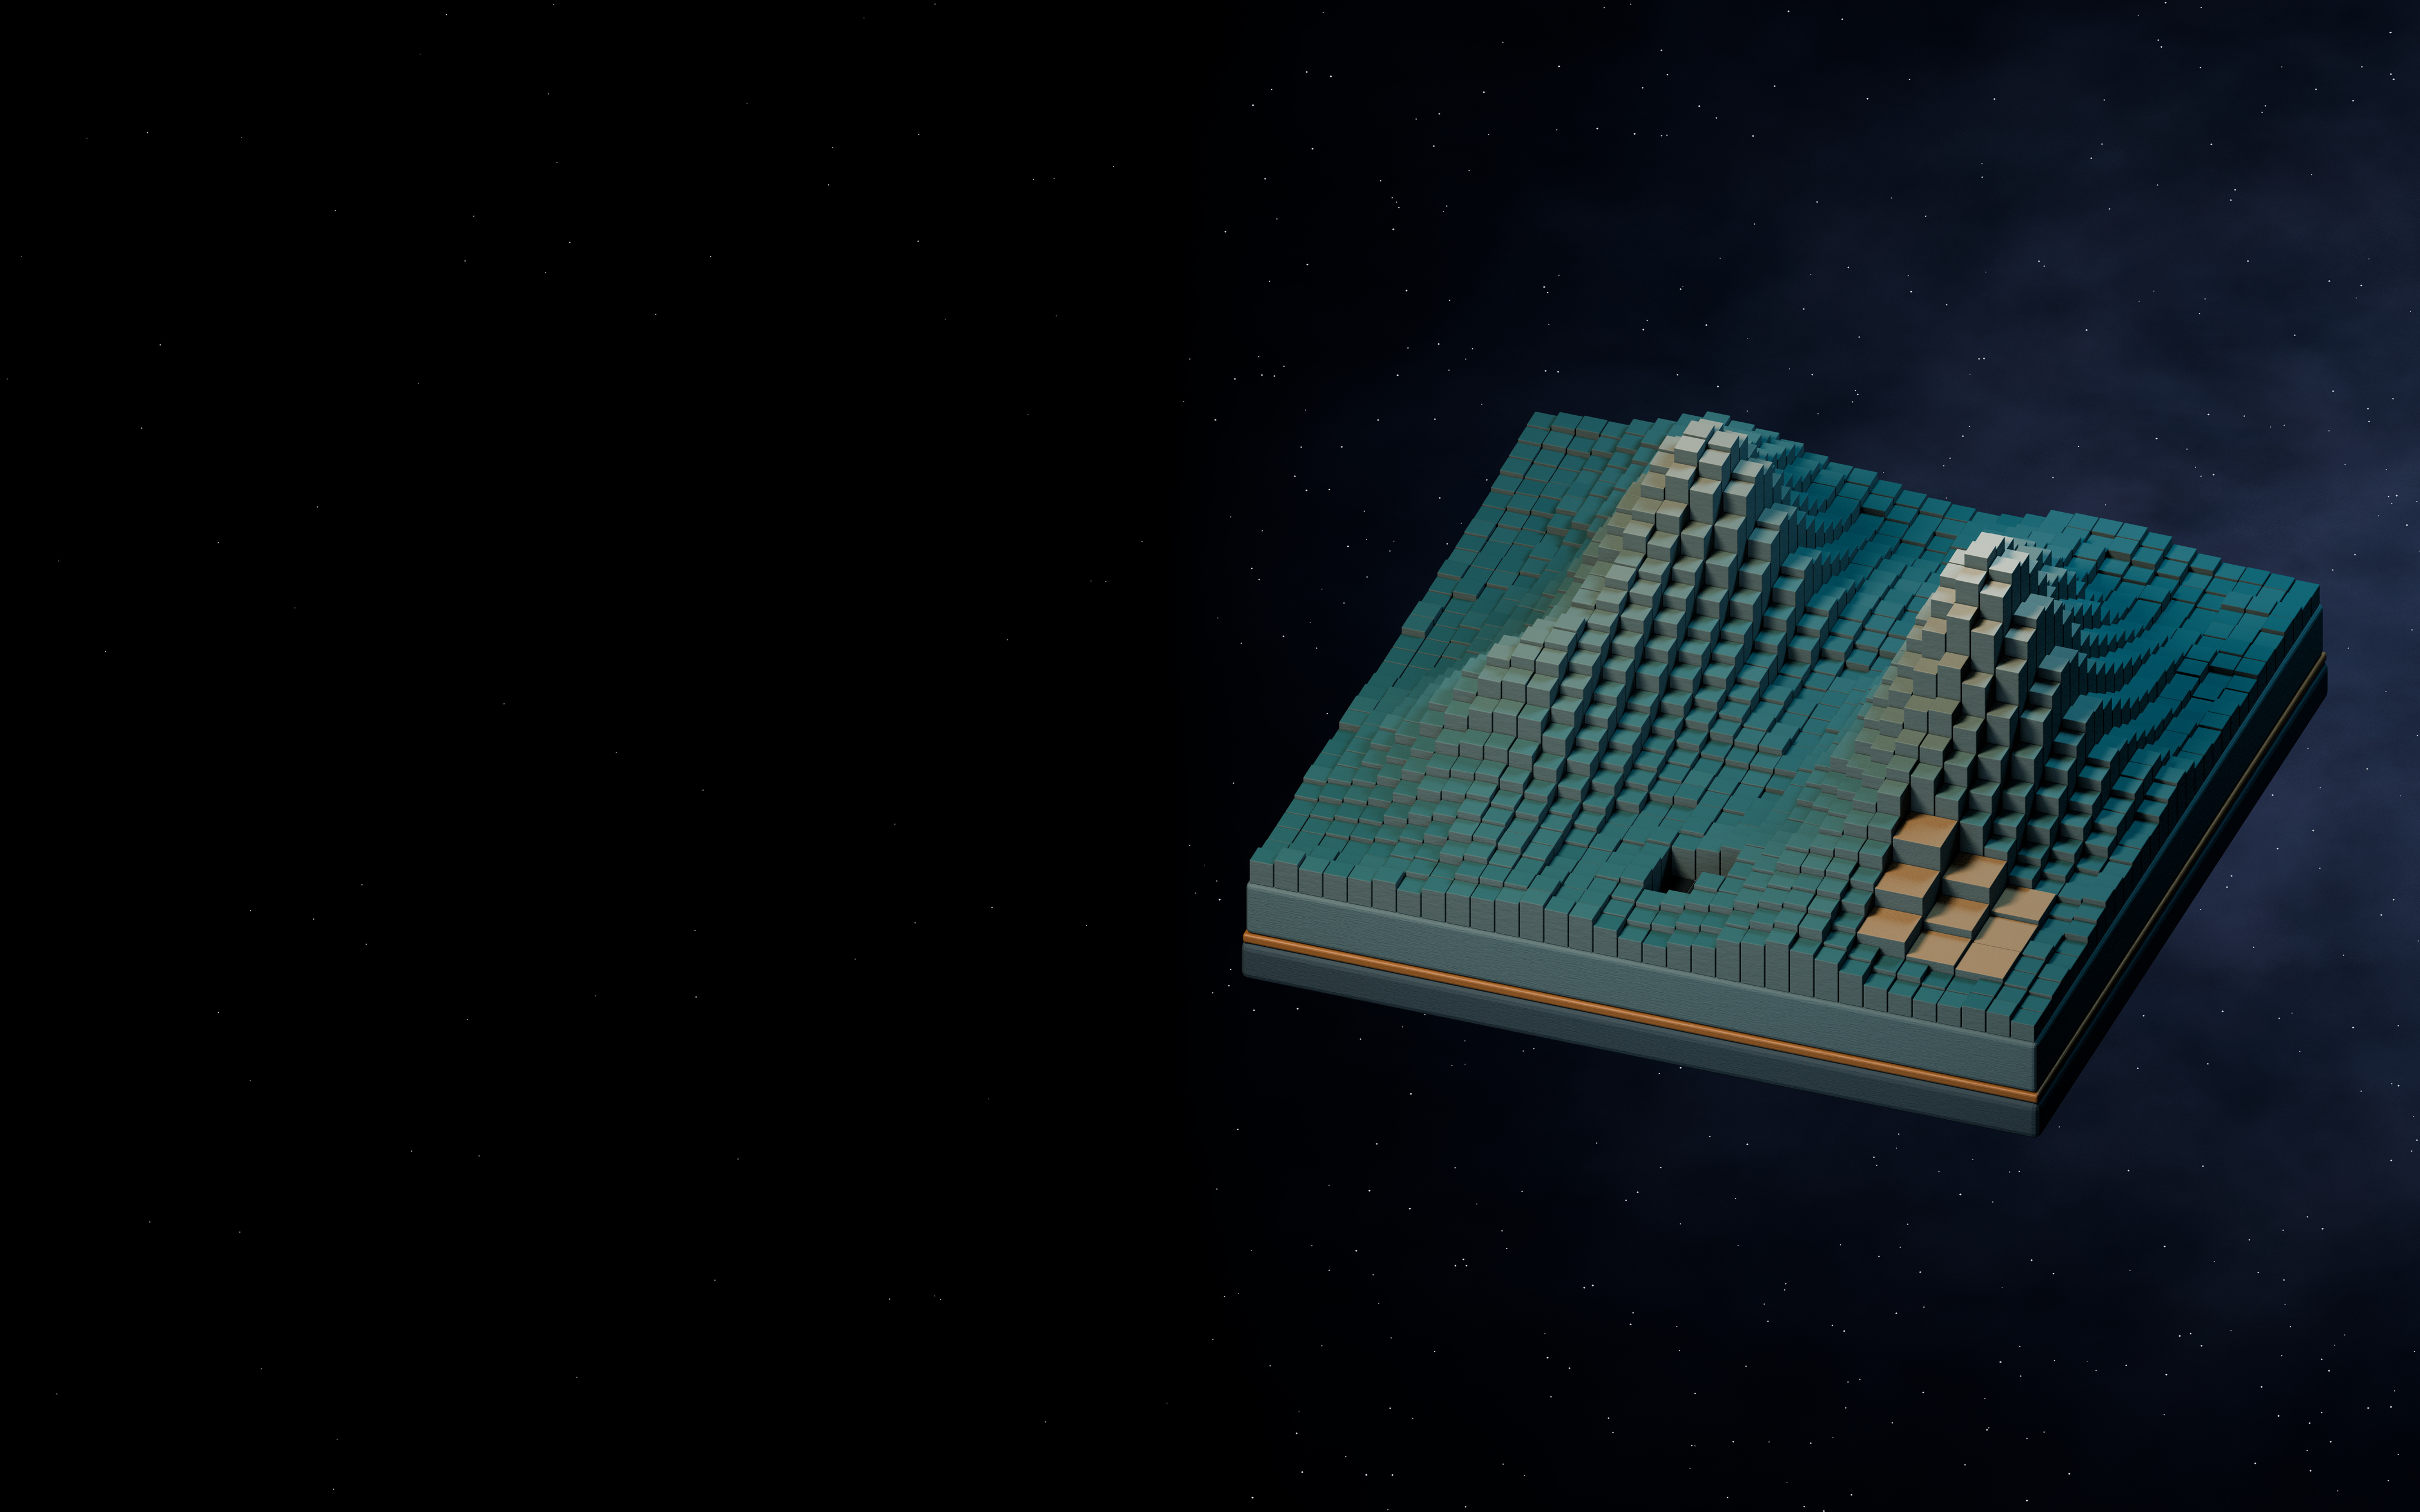
\includegraphics[width=20cm,height=12.5cm]{Risorse/Copertine/M12_Tessera.jpg}};}{}
\node[anchor=north west,inner sep=0] at([xshift=1.05cm,yshift=-1.10cm]current page.north west){\color{Mint}\bfseries\fontsize{23}{28}\selectfont TESSERA};
\node[anchor=north west,inner sep=0] at([xshift=1.07cm,yshift=-2.16cm]current page.north west){\color{white}\fontsize{9}{12}\selectfont MODULO M12 · SCIENZE DELLA TERRA};
\draw[Mint,line width=1.5pt]([xshift=1.07cm,yshift=-2.78cm]current page.north west)--([xshift=2.6cm,yshift=-2.78cm]current page.north west);
\node[anchor=north west,inner sep=0] at([xshift=1.05cm,yshift=-3.35cm]current page.north west){\begin{minipage}{9.2cm}\raggedright\color{white}\bfseries\fontsize{28.5}{34.5}\selectfont Raster,\\telerilevamento\\e morfometria\end{minipage}};
\node[anchor=north west,inner sep=0] at([xshift=1.07cm,yshift=-7.88cm]current page.north west){\begin{minipage}{8.9cm}\raggedright\color{Lilac}\fontsize{12.2}{17}\selectfont Celle e forme del paesaggio\end{minipage}};
\node[anchor=north west,inner sep=0] at([xshift=1.07cm,yshift=-8.70cm]current page.north west){\begin{minipage}{8.9cm}\raggedright\color{white!75}\fontsize{10.3}{14.5}\selectfont Dalla geometria della griglia\\alle grandezze derivate\end{minipage}};
\node[anchor=north west,inner sep=0] at([xshift=1.07cm,yshift=-10.52cm]current page.north west){\color{white}\fontsize{11.5}{15}\selectfont Marzio De Corato};
\node[anchor=north west,inner sep=0] at([xshift=1.07cm,yshift=-11.17cm]current page.north west){\color{Mint}\fontsize{8.8}{11}\selectfont\href{https://creativecommons.org/licenses/by-nc-sa/4.0/}{© 2026 · CC BY-NC-SA 4.0}};
\end{tikzpicture}\end{frame}
\begin{frame}[plain]\hypertarget{slide2}{}
\bookmark[level=0,page=2]{I · TERRITORIO E GRIGLIA}
\bookmark[level=1,page=2]{Dalle celle alle grandezze derivate}
\begin{lrbox}{\TitleBox}
\begin{minipage}[t]{17.7cm}\raggedright\color{Ink}\fontsize{11.3}{14.8}\selectfont
\color{Navy}\bfseries\fontsize{20.6}{24.5}\selectfont Dalle celle alle grandezze derivate
\end{minipage}\end{lrbox}
\typeout{FULLBOX:002:TitleBox:\the\ht\TitleBox:\the\dp\TitleBox}

\begin{lrbox}{\RecallBox}
\begin{minipage}[t]{14.3cm}\raggedright\color{Ink}\fontsize{11.3}{14.8}\selectfont
\fontsize{10.3}{13.8}\selectfont La geometria della griglia entra nel significato dei valori e delle grandezze derivate.
\end{minipage}\end{lrbox}
\typeout{FULLBOX:002:RecallBox:\the\ht\RecallBox:\the\dp\RecallBox}

\begin{lrbox}{\PilotLeftBox}
\begin{minipage}[t]{10.05cm}\raggedright\color{Ink}\fontsize{11.3}{14.8}\selectfont
\PLabel{Il percorso di Tessera}
{\fontsize{10.2}{13.1}\selectfont\renewcommand{\arraystretch}{1.45}\begin{tabular}{@{}p{8.3cm}p{0.7cm}@{}}\toprule
\textbf{Passaggio} & \textbf{p.}\\\midrule
\hyperlink{slide6}{Definire la geometria raster} & 6\\
\hyperlink{slide20}{Conservare maschere e dominio} & 20\\
\hyperlink{slide33}{Cambiare risoluzione e allineare} & 33\\
\hyperlink{slide49}{Calcolare e verificare le derivate} & 49\\
\hyperlink{slide67}{Illuminare il rilievo} & 67\\
\hyperlink{slide77}{Confrontare bande spettrali} & 77\\
\hyperlink{slide91}{Riassumere zone e dipendenza} & 91\\
\hyperlink{slide103}{Esportare e rileggere i risultati} & 103\\
\bottomrule\end{tabular}}

\end{minipage}\end{lrbox}
\typeout{FULLBOX:002:PilotLeftBox:\the\ht\PilotLeftBox:\the\dp\PilotLeftBox}

\begin{lrbox}{\PilotRightBox}
\begin{minipage}[t]{7.55cm}\raggedright\color{Ink}\fontsize{11.3}{14.8}\selectfont
\PBody{Locus ha collegato campioni, posizioni e relazioni spaziali. Tessera segue i valori quando il territorio è rappresentato da una griglia.}
\vspace{2.5mm}
\PInfo{Il caso guida è un terreno sintetico di 24 righe e 30 colonne. La georeferenziazione del GeoTIFF è fittizia: il file serve a verificare operazioni e convenzioni.}
\PBody{I 20 notebook conservano gli identificativi M12\_N01--M12\_N20. Ogni attività collega un problema, il codice eseguito e una conclusione circoscritta.}
\vspace{2.5mm}

\end{minipage}\end{lrbox}
\typeout{FULLBOX:002:PilotRightBox:\the\ht\PilotRightBox:\the\dp\PilotRightBox}

\begin{tikzpicture}[remember picture,overlay]
\PilotChrome{Dalle celle alle grandezze derivate}{I · TERRITORIO E GRIGLIA}{2}{La geometria della griglia entra nel significato dei valori e delle grandezze derivate.}
\node[anchor=north west,inner sep=0] at([xshift=.96cm,yshift=-2.13cm]current page.north west){\usebox{\PilotLeftBox}};
\node[anchor=north west,inner sep=0] at([xshift=11.52cm,yshift=-2.13cm]current page.north west){\usebox{\PilotRightBox}};
\end{tikzpicture}\end{frame}

\begin{frame}[plain]\hypertarget{slide3}{}
\bookmark[level=1,page=3]{Dai campioni di Locus alle celle di Tessera}
\begin{lrbox}{\TitleBox}
\begin{minipage}[t]{17.7cm}\raggedright\color{Ink}\fontsize{11.3}{14.8}\selectfont
\color{Navy}\bfseries\fontsize{20.6}{24.5}\selectfont Dai campioni di Locus alle celle di Tessera
\end{minipage}\end{lrbox}
\typeout{FULLBOX:003:TitleBox:\the\ht\TitleBox:\the\dp\TitleBox}

\begin{lrbox}{\RecallBox}
\begin{minipage}[t]{14.3cm}\raggedright\color{Ink}\fontsize{11.3}{14.8}\selectfont
\fontsize{10.3}{13.8}\selectfont La continuità della carta è una proprietà della rappresentazione da interpretare insieme al dato.
\end{minipage}\end{lrbox}
\typeout{FULLBOX:003:RecallBox:\the\ht\RecallBox:\the\dp\RecallBox}

\begin{lrbox}{\PilotLeftBox}
\begin{minipage}[t]{10.05cm}\raggedright\color{Ink}\fontsize{11.3}{14.8}\selectfont
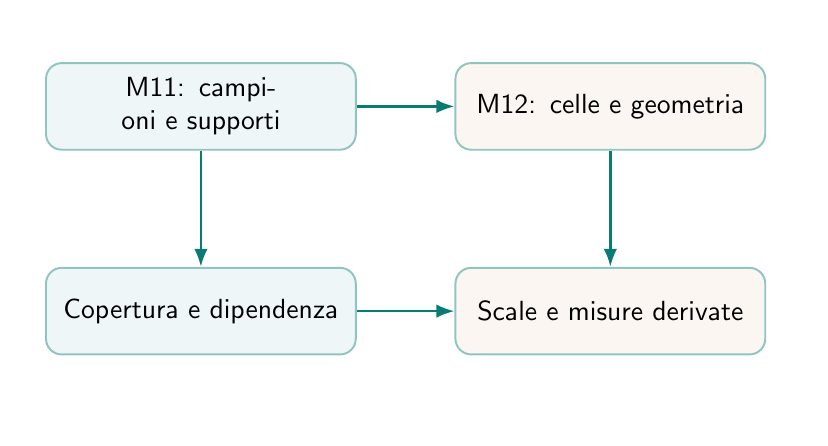
\begin{tikzpicture}[x=1cm,y=1cm]
\path[use as bounding box](-.1,-.15) rectangle(9.7,4.8);
\node[pFlow,text width=3.7cm,fill=GeoA!7] (a) at(2.1,3.8){M11: campioni e supporti};
\node[pFlow,text width=3.7cm,fill=GeoB!7] (b) at(7.3,3.8){M12: celle e geometria};
\node[pFlow,text width=3.7cm,fill=GeoA!7] (c) at(2.1,1.2){Copertura e dipendenza};
\node[pFlow,text width=3.7cm,fill=GeoB!7] (d) at(7.3,1.2){Scale e misure derivate};
\draw[pEdge] (a) -- (b);
\draw[pEdge] (a) -- (c);
\draw[pEdge] (b) -- (d);
\draw[pEdge] (c) -- (d);
\end{tikzpicture}
\[Z(s)\quad\longrightarrow\quad Z_{ij}\text{ su una griglia dichiarata}\]

\end{minipage}\end{lrbox}
\typeout{FULLBOX:003:PilotLeftBox:\the\ht\PilotLeftBox:\the\dp\PilotLeftBox}

\begin{lrbox}{\PilotRightBox}
\begin{minipage}[t]{7.55cm}\raggedright\color{Ink}\fontsize{11.3}{14.8}\selectfont
\PBody{Un raster organizza il dominio in celle. Il valore di ogni cella può essere una misura, una categoria, una previsione o una sintesi su un supporto.}
\vspace{2.5mm}
\PInfo{La disposizione regolare facilita il calcolo, ma non rende indipendenti le osservazioni e non garantisce che ogni cella contenga una misura diretta.}
\PBody{Coordinate, supporto e provenienza restano necessari anche quando la superficie appare continua sullo schermo.}
\vspace{2.5mm}

\end{minipage}\end{lrbox}
\typeout{FULLBOX:003:PilotRightBox:\the\ht\PilotRightBox:\the\dp\PilotRightBox}

\begin{tikzpicture}[remember picture,overlay]
\PilotChrome{Dai campioni di Locus alle celle di Tessera}{I · TERRITORIO E GRIGLIA}{3}{La continuità della carta è una proprietà della rappresentazione da interpretare insieme al dato.}
\node[anchor=north west,inner sep=0] at([xshift=.96cm,yshift=-2.13cm]current page.north west){\usebox{\PilotLeftBox}};
\node[anchor=north west,inner sep=0] at([xshift=11.52cm,yshift=-2.13cm]current page.north west){\usebox{\PilotRightBox}};
\end{tikzpicture}\end{frame}

\begin{frame}[plain]\hypertarget{slide4}{}
\bookmark[level=1,page=4]{Quattro domande prima del calcolo}
\begin{lrbox}{\TitleBox}
\begin{minipage}[t]{17.7cm}\raggedright\color{Ink}\fontsize{11.3}{14.8}\selectfont
\color{Navy}\bfseries\fontsize{20.6}{24.5}\selectfont Quattro domande prima del calcolo
\end{minipage}\end{lrbox}
\typeout{FULLBOX:004:TitleBox:\the\ht\TitleBox:\the\dp\TitleBox}

\begin{lrbox}{\RecallBox}
\begin{minipage}[t]{14.3cm}\raggedright\color{Ink}\fontsize{11.3}{14.8}\selectfont
\fontsize{10.3}{13.8}\selectfont Prima dell’algoritmo occorre dichiarare geometria, significato dei valori e dominio valido.
\end{minipage}\end{lrbox}
\typeout{FULLBOX:004:RecallBox:\the\ht\RecallBox:\the\dp\RecallBox}

\begin{lrbox}{\PilotLeftBox}
\begin{minipage}[t]{10.05cm}\raggedright\color{Ink}\fontsize{11.3}{14.8}\selectfont
{\fontsize{10.2}{13.1}\selectfont\renewcommand{\arraystretch}{1.45}\begin{tabular}{@{}p{4.1cm}p{4.9cm}@{}}\toprule
\textbf{Domanda} & \textbf{Evidenza da conservare}\\\midrule
Dove si trova ogni cella? & Riferimento, origine, passo e orientamento\\
Che cosa significa il valore? & Variabile, unità, supporto e provenienza\\
Quali celle sono valide? & Maschere, cause di esclusione e dominio\\
Come cambia il risultato? & Metodo, parametri e scala di elaborazione\\
\bottomrule\end{tabular}}

\end{minipage}\end{lrbox}
\typeout{FULLBOX:004:PilotLeftBox:\the\ht\PilotLeftBox:\the\dp\PilotLeftBox}

\begin{lrbox}{\PilotRightBox}
\begin{minipage}[t]{7.55cm}\raggedright\color{Ink}\fontsize{11.3}{14.8}\selectfont
\PBody{La stessa matrice numerica può essere collocata in luoghi differenti. La stessa immagine può mostrare quote, intensità luminose oppure un indice spettrale.}
\vspace{2.5mm}
\PInfo{Il progetto conserverà dati, griglia e regole di trasformazione. La verifica finale rileggerà anche i file esportati.}
\PBody{La copertina richiama celle e forme del paesaggio. Nelle figure scientifiche ogni colore e ogni misura avranno unità e metodo espliciti.}
\vspace{2.5mm}

\end{minipage}\end{lrbox}
\typeout{FULLBOX:004:PilotRightBox:\the\ht\PilotRightBox:\the\dp\PilotRightBox}

\begin{tikzpicture}[remember picture,overlay]
\PilotChrome{Quattro domande prima del calcolo}{I · TERRITORIO E GRIGLIA}{4}{Prima dell’algoritmo occorre dichiarare geometria, significato dei valori e dominio valido.}
\node[anchor=north west,inner sep=0] at([xshift=.96cm,yshift=-2.13cm]current page.north west){\usebox{\PilotLeftBox}};
\node[anchor=north west,inner sep=0] at([xshift=11.52cm,yshift=-2.13cm]current page.north west){\usebox{\PilotRightBox}};
\end{tikzpicture}\end{frame}

\begin{frame}[plain]\hypertarget{slide5}{}
\bookmark[level=1,page=5]{Il caso guida: 720 celle di terreno sintetico}
\begin{lrbox}{\TitleBox}
\begin{minipage}[t]{17.7cm}\raggedright\color{Ink}\fontsize{11.3}{14.8}\selectfont
\color{Navy}\bfseries\fontsize{20.6}{24.5}\selectfont Il caso guida: 720 celle di terreno sintetico
\end{minipage}\end{lrbox}
\typeout{FULLBOX:005:TitleBox:\the\ht\TitleBox:\the\dp\TitleBox}

\begin{lrbox}{\RecallBox}
\begin{minipage}[t]{14.3cm}\raggedright\color{Ink}\fontsize{11.3}{14.8}\selectfont
\fontsize{10.3}{13.8}\selectfont Un caso sintetico rende verificabili i passaggi senza attribuire ai risultati una provenienza osservativa.
\end{minipage}\end{lrbox}
\typeout{FULLBOX:005:RecallBox:\the\ht\RecallBox:\the\dp\RecallBox}

\begin{lrbox}{\PilotLeftBox}
\begin{minipage}[t]{10.05cm}\raggedright\color{Ink}\fontsize{11.3}{14.8}\selectfont
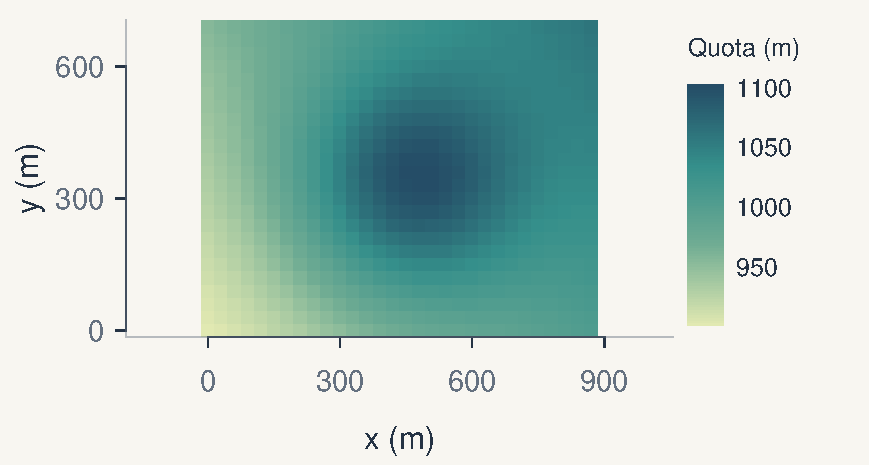
\includegraphics[width=9.85cm,height=5.25cm,keepaspectratio]{Risultati/Figure/01_dem.pdf}
\vspace{1.5mm}
\PSmall{24 righe, 30 colonne, passo 30 m. I centri locali vanno da 0 a 870 m verso Est e da 0 a 690 m verso Nord.}

\end{minipage}\end{lrbox}
\typeout{FULLBOX:005:PilotLeftBox:\the\ht\PilotLeftBox:\the\dp\PilotLeftBox}

\begin{lrbox}{\PilotRightBox}
\begin{minipage}[t]{7.55cm}\raggedright\color{Ink}\fontsize{11.3}{14.8}\selectfont
\PBody{Il file contiene quota e appartenenza alle zone didattiche A e B. Le bande spettrali saranno costruite in un esperimento distinto.}
\vspace{2.5mm}
\PInfo{Le quote non sono misure di un rilievo reale. La collocazione UTM del GeoTIFF è convenzionale e non coincide con i siti di Locus.}
\PBody{Il terreno consente di riconoscere errori di orientamento, modifiche della scala e conseguenze del trattamento dei mancanti.}
\vspace{2.5mm}

\end{minipage}\end{lrbox}
\typeout{FULLBOX:005:PilotRightBox:\the\ht\PilotRightBox:\the\dp\PilotRightBox}

\begin{tikzpicture}[remember picture,overlay]
\PilotChrome{Il caso guida: 720 celle di terreno sintetico}{I · TERRITORIO E GRIGLIA}{5}{Un caso sintetico rende verificabili i passaggi senza attribuire ai risultati una provenienza osservativa.}
\node[anchor=north west,inner sep=0] at([xshift=.96cm,yshift=-2.13cm]current page.north west){\usebox{\PilotLeftBox}};
\node[anchor=north west,inner sep=0] at([xshift=11.52cm,yshift=-2.13cm]current page.north west){\usebox{\PilotRightBox}};
\node[anchor=north east,inner sep=0] at([xshift=17.65cm,yshift=-12.06cm]current page.north west){\color{Classical}\fontsize{7.7}{9.2}\selectfont\href{../../03_Notebook_svolti/M12_Tessera/M12_N01.html}{M12\_N01 · notebook svolto}};
\end{tikzpicture}\end{frame}

\begin{frame}[plain]\hypertarget{slide6}{}
\bookmark[level=0,page=6]{II · GEOMETRIA RASTER}
\bookmark[level=1,page=6]{Il raster conserva valori e geometria}
\begin{lrbox}{\TitleBox}
\begin{minipage}[t]{17.7cm}\raggedright\color{Ink}\fontsize{11.3}{14.8}\selectfont
\color{Navy}\bfseries\fontsize{20.6}{24.5}\selectfont Il raster conserva valori e geometria
\end{minipage}\end{lrbox}
\typeout{FULLBOX:006:TitleBox:\the\ht\TitleBox:\the\dp\TitleBox}

\begin{lrbox}{\RecallBox}
\begin{minipage}[t]{14.3cm}\raggedright\color{Ink}\fontsize{11.3}{14.8}\selectfont
\fontsize{10.3}{13.8}\selectfont Numero di valori e dimensioni della matrice non identificano da soli un raster.
\end{minipage}\end{lrbox}
\typeout{FULLBOX:006:RecallBox:\the\ht\RecallBox:\the\dp\RecallBox}

\begin{lrbox}{\PilotLeftBox}
\begin{minipage}[t]{10.05cm}\raggedright\color{Ink}\fontsize{11.3}{14.8}\selectfont
{\fontsize{10.2}{13.1}\selectfont\renewcommand{\arraystretch}{1.45}\begin{tabular}{@{}p{4.2cm}p{4.8cm}@{}}\toprule
\textbf{Elemento} & \textbf{Nel caso guida}\\\midrule
Dimensioni & 24 righe e 30 colonne\\
Passo della griglia & 30 m lungo entrambi gli assi\\
Valori & Quote sintetiche in metri\\
Georeferenziazione & UTM 32N convenzionale, EPSG:32632\\
Variabile categoriale & Zone sintetiche A e B\\
Mancanti & Regola NoData dichiarata nel file\\
\bottomrule\end{tabular}}

\end{minipage}\end{lrbox}
\typeout{FULLBOX:006:PilotLeftBox:\the\ht\PilotLeftBox:\the\dp\PilotLeftBox}

\begin{lrbox}{\PilotRightBox}
\begin{minipage}[t]{7.55cm}\raggedright\color{Ink}\fontsize{11.3}{14.8}\selectfont
\PBody{La matrice raccoglie i valori. Origine, risoluzione, riferimento e orientamento stabiliscono la posizione delle celle.}
\vspace{2.5mm}
\PInfo{Due oggetti con 720 valori possono rappresentare griglie diverse. Confrontiamo i metadati prima di combinarli.}
\PSmall{Gli originali sono conservati con revisione Git e impronte verificabili nel pacchetto.}

\end{minipage}\end{lrbox}
\typeout{FULLBOX:006:PilotRightBox:\the\ht\PilotRightBox:\the\dp\PilotRightBox}

\begin{tikzpicture}[remember picture,overlay]
\PilotChrome{Il raster conserva valori e geometria}{II · GEOMETRIA RASTER}{6}{Numero di valori e dimensioni della matrice non identificano da soli un raster.}
\node[anchor=north west,inner sep=0] at([xshift=.96cm,yshift=-2.13cm]current page.north west){\usebox{\PilotLeftBox}};
\node[anchor=north west,inner sep=0] at([xshift=11.52cm,yshift=-2.13cm]current page.north west){\usebox{\PilotRightBox}};
\node[anchor=north east,inner sep=0] at([xshift=17.65cm,yshift=-12.06cm]current page.north west){\color{Classical}\fontsize{7.7}{9.2}\selectfont\href{../../03_Notebook_svolti/M12_Tessera/M12_N01.html}{M12\_N01 · notebook svolto}};
\end{tikzpicture}\end{frame}

\begin{frame}[plain]\hypertarget{slide7}{}
\bookmark[level=1,page=7]{Righe e colonne diventano posizioni}
\begin{lrbox}{\TitleBox}
\begin{minipage}[t]{17.7cm}\raggedright\color{Ink}\fontsize{11.3}{14.8}\selectfont
\color{Navy}\bfseries\fontsize{20.6}{24.5}\selectfont Righe e colonne diventano posizioni
\end{minipage}\end{lrbox}
\typeout{FULLBOX:007:TitleBox:\the\ht\TitleBox:\the\dp\TitleBox}

\begin{lrbox}{\RecallBox}
\begin{minipage}[t]{14.3cm}\raggedright\color{Ink}\fontsize{11.3}{14.8}\selectfont
\fontsize{10.3}{13.8}\selectfont Gli indici descrivono l’ordine in tabella; le coordinate descrivono la geometria dichiarata.
\end{minipage}\end{lrbox}
\typeout{FULLBOX:007:RecallBox:\the\ht\RecallBox:\the\dp\RecallBox}

\begin{lrbox}{\PilotLeftBox}
\begin{minipage}[t]{10.05cm}\raggedright\color{Ink}\fontsize{11.3}{14.8}\selectfont
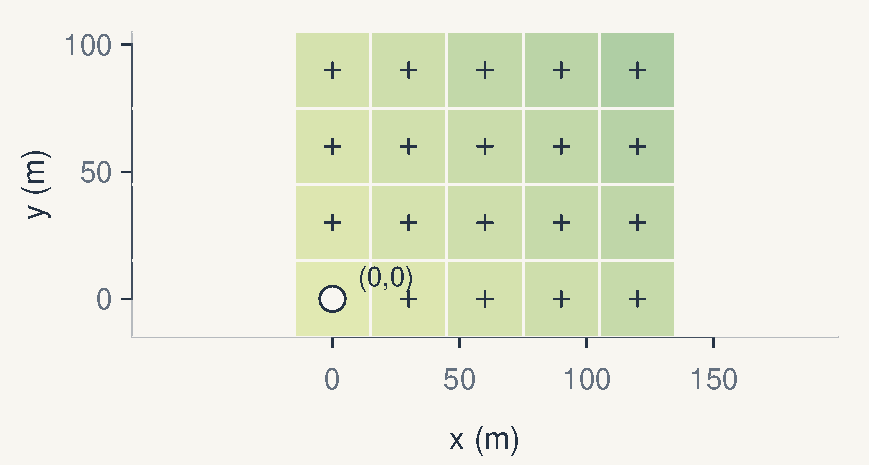
\includegraphics[width=9.85cm,height=4.65cm,keepaspectratio]{Risultati/Figure/03_celle_centri.pdf}
\vspace{1.5mm}
\PSmall{Dettaglio del raster locale: croci nei centri, bordi a mezzo passo. La cella centrata in $(0,0)$ si estende da −15 a 15 m sui due assi.}
\[x_j=x_0+j\Delta x,\qquad y_i=y_0+i\Delta y\]

\end{minipage}\end{lrbox}
\typeout{FULLBOX:007:PilotLeftBox:\the\ht\PilotLeftBox:\the\dp\PilotLeftBox}

\begin{lrbox}{\PilotRightBox}
\begin{minipage}[t]{7.55cm}\raggedright\color{Ink}\fontsize{11.3}{14.8}\selectfont
\PBody{Nella tabella originale gli indici partono da zero. Il centro della cella $(0,0)$ ha coordinate locali $(0,0)$ m.}
\vspace{2.5mm}
\PInfo{Qui $x$ cresce verso Est e $y$ verso Nord. Una convenzione diversa per le righe richiederebbe un segno diverso nella seconda relazione.}
\PBody{La griglia disegnata è uno schema: il dataset completo contiene 24 righe e 30 colonne.}
\vspace{2.5mm}

\end{minipage}\end{lrbox}
\typeout{FULLBOX:007:PilotRightBox:\the\ht\PilotRightBox:\the\dp\PilotRightBox}

\begin{tikzpicture}[remember picture,overlay]
\PilotChrome{Righe e colonne diventano posizioni}{II · GEOMETRIA RASTER}{7}{Gli indici descrivono l’ordine in tabella; le coordinate descrivono la geometria dichiarata.}
\node[anchor=north west,inner sep=0] at([xshift=.96cm,yshift=-2.13cm]current page.north west){\usebox{\PilotLeftBox}};
\node[anchor=north west,inner sep=0] at([xshift=11.52cm,yshift=-2.13cm]current page.north west){\usebox{\PilotRightBox}};
\node[anchor=north east,inner sep=0] at([xshift=17.65cm,yshift=-12.06cm]current page.north west){\color{Classical}\fontsize{7.7}{9.2}\selectfont\href{../../03_Notebook_svolti/M12_Tessera/M12_N01.html}{M12\_N01 · notebook svolto}};
\end{tikzpicture}\end{frame}

\begin{frame}[plain]\hypertarget{slide8}{}
\bookmark[level=1,page=8]{Il centro della cella e il suo angolo sono distinti}
\begin{lrbox}{\TitleBox}
\begin{minipage}[t]{17.7cm}\raggedright\color{Ink}\fontsize{11.3}{14.8}\selectfont
\color{Navy}\bfseries\fontsize{20.6}{24.5}\selectfont Il centro della cella e il suo angolo sono distinti
\end{minipage}\end{lrbox}
\typeout{FULLBOX:008:TitleBox:\the\ht\TitleBox:\the\dp\TitleBox}

\begin{lrbox}{\RecallBox}
\begin{minipage}[t]{14.3cm}\raggedright\color{Ink}\fontsize{11.3}{14.8}\selectfont
\fontsize{10.3}{13.8}\selectfont Origine degli angoli e coordinate dei centri devono essere riconoscibili nei metadati.
\end{minipage}\end{lrbox}
\typeout{FULLBOX:008:RecallBox:\the\ht\RecallBox:\the\dp\RecallBox}

\begin{lrbox}{\PilotLeftBox}
\begin{minipage}[t]{10.05cm}\raggedright\color{Ink}\fontsize{11.3}{14.8}\selectfont
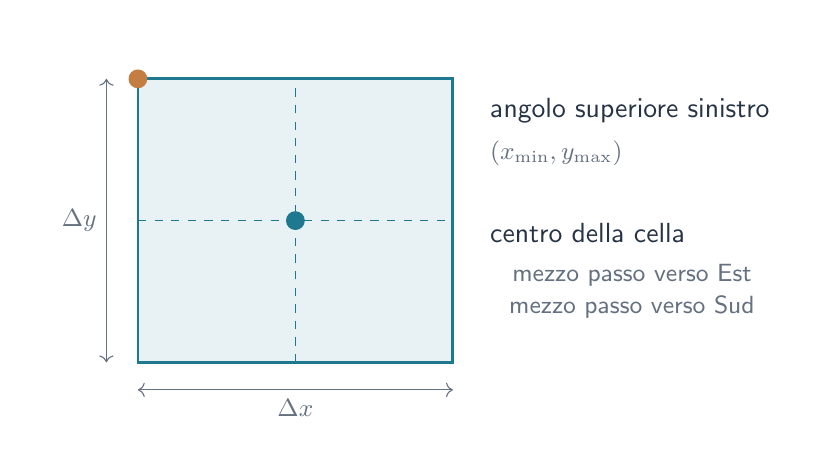
\begin{tikzpicture}[x=1cm,y=1cm]
\path[use as bounding box](-.1,-.15) rectangle(9.7,5.15);
\filldraw[fill=GeoA!10,draw=GeoA,line width=1pt](1.3,.9)rectangle(5.3,4.5);
\fill[GeoB](1.3,4.5)circle(3.4pt);
\fill[GeoA](3.3,2.7)circle(3.4pt);
\draw[GeoA,dashed](3.3,.9)--(3.3,4.5);
\draw[GeoA,dashed](1.3,2.7)--(5.3,2.7);
\draw[<->,draw=Muted](1.3,.55)--node[below,pNote]{$\Delta x$}(5.3,.55);
\draw[<->,draw=Muted](.9,.9)--node[left,pNote]{$\Delta y$}(.9,4.5);
\node[pLabel,anchor=west]at(5.65,4.1){angolo superiore sinistro};
\node[pNote,anchor=west]at(5.65,3.55){$(x_{\min},y_{\max})$};
\node[pLabel,anchor=west]at(5.65,2.55){centro della cella};
\node[pNote,anchor=west,text width=3.6cm]at(5.65,1.8){mezzo passo verso Est\\mezzo passo verso Sud};
\end{tikzpicture}

\end{minipage}\end{lrbox}
\typeout{FULLBOX:008:PilotLeftBox:\the\ht\PilotLeftBox:\the\dp\PilotLeftBox}

\begin{lrbox}{\PilotRightBox}
\begin{minipage}[t]{7.55cm}\raggedright\color{Ink}\fontsize{11.3}{14.8}\selectfont
\PBody{La georeferenziazione del GeoTIFF parte dall’angolo superiore sinistro della cella in alto a sinistra. Il centro si trova mezzo passo all’interno.}
\vspace{2.5mm}
\PInfo{Con celle di 30 m, la differenza è 15 m in ciascuna direzione. Confondere angolo e centro sposta l’intera griglia di mezzo pixel.}
\PBody{Nel file originale la convenzione è PixelIsArea. Il significato fisico del valore dipende comunque dal prodotto e dalla sua documentazione.}
\vspace{2.5mm}

\end{minipage}\end{lrbox}
\typeout{FULLBOX:008:PilotRightBox:\the\ht\PilotRightBox:\the\dp\PilotRightBox}

\begin{tikzpicture}[remember picture,overlay]
\PilotChrome{Il centro della cella e il suo angolo sono distinti}{II · GEOMETRIA RASTER}{8}{Origine degli angoli e coordinate dei centri devono essere riconoscibili nei metadati.}
\node[anchor=north west,inner sep=0] at([xshift=.96cm,yshift=-2.13cm]current page.north west){\usebox{\PilotLeftBox}};
\node[anchor=north west,inner sep=0] at([xshift=11.52cm,yshift=-2.13cm]current page.north west){\usebox{\PilotRightBox}};
\node[anchor=north east,inner sep=0] at([xshift=17.65cm,yshift=-12.06cm]current page.north west){\color{Classical}\fontsize{7.7}{9.2}\selectfont\href{../../03_Notebook_svolti/M12_Tessera/M12_N03.html}{M12\_N03 · notebook svolto}};
\end{tikzpicture}\end{frame}

\begin{frame}[plain]\hypertarget{slide9}{}
\bookmark[level=1,page=9]{La prima riga del GeoTIFF si trova a Nord}
\begin{lrbox}{\TitleBox}
\begin{minipage}[t]{17.7cm}\raggedright\color{Ink}\fontsize{11.3}{14.8}\selectfont
\color{Navy}\bfseries\fontsize{20.6}{24.5}\selectfont La prima riga del GeoTIFF si trova a Nord
\end{minipage}\end{lrbox}
\typeout{FULLBOX:009:TitleBox:\the\ht\TitleBox:\the\dp\TitleBox}

\begin{lrbox}{\RecallBox}
\begin{minipage}[t]{14.3cm}\raggedright\color{Ink}\fontsize{11.3}{14.8}\selectfont
\fontsize{10.3}{13.8}\selectfont La formula dei centri dipende dal punto di origine e dall’orientamento delle righe.
\end{minipage}\end{lrbox}
\typeout{FULLBOX:009:RecallBox:\the\ht\RecallBox:\the\dp\RecallBox}

\begin{lrbox}{\PilotLeftBox}
\begin{minipage}[t]{10.05cm}\raggedright\color{Ink}\fontsize{11.3}{14.8}\selectfont
\[E_j=E_{\min}+\left(j+\tfrac12\right)\Delta x\]
\[N_i=N_{\max}-\left(i+\tfrac12\right)\Delta y\]
\PInfo{Indici $i,j$ da zero. Griglia senza rotazione: $E$ cresce verso Est, $N$ verso Nord; il numero di riga aumenta andando verso Sud.}

\end{minipage}\end{lrbox}
\typeout{FULLBOX:009:PilotLeftBox:\the\ht\PilotLeftBox:\the\dp\PilotLeftBox}

\begin{lrbox}{\PilotRightBox}
\begin{minipage}[t]{7.55cm}\raggedright\color{Ink}\fontsize{11.3}{14.8}\selectfont
\PBody{Il file ha angolo superiore sinistro $(500000,5000000)$ m. Il primo centro è quindi $(500015,4999985)$ m.}
\vspace{2.5mm}
\PBody{Il segno meno nella coordinata Nord è una conseguenza dell’ordine delle righe. Non indica una distanza fisica negativa.}
\vspace{2.5mm}
\PSmall{Per griglie ruotate la trasformazione affine comprende anche i termini incrociati fra riga e colonna.}

\end{minipage}\end{lrbox}
\typeout{FULLBOX:009:PilotRightBox:\the\ht\PilotRightBox:\the\dp\PilotRightBox}

\begin{tikzpicture}[remember picture,overlay]
\PilotChrome{La prima riga del GeoTIFF si trova a Nord}{II · GEOMETRIA RASTER}{9}{La formula dei centri dipende dal punto di origine e dall’orientamento delle righe.}
\node[anchor=north west,inner sep=0] at([xshift=.96cm,yshift=-2.13cm]current page.north west){\usebox{\PilotLeftBox}};
\node[anchor=north west,inner sep=0] at([xshift=11.52cm,yshift=-2.13cm]current page.north west){\usebox{\PilotRightBox}};
\node[anchor=north east,inner sep=0] at([xshift=17.65cm,yshift=-12.06cm]current page.north west){\color{Classical}\fontsize{7.7}{9.2}\selectfont\href{../../03_Notebook_svolti/M12_Tessera/M12_N03.html}{M12\_N03 · notebook svolto}};
\end{tikzpicture}\end{frame}

\begin{frame}[plain]\hypertarget{slide10}{}
\bookmark[level=1,page=10]{L’estensione comprende celle intere}
\begin{lrbox}{\TitleBox}
\begin{minipage}[t]{17.7cm}\raggedright\color{Ink}\fontsize{11.3}{14.8}\selectfont
\color{Navy}\bfseries\fontsize{20.6}{24.5}\selectfont L’estensione comprende celle intere
\end{minipage}\end{lrbox}
\typeout{FULLBOX:010:TitleBox:\the\ht\TitleBox:\the\dp\TitleBox}

\begin{lrbox}{\RecallBox}
\begin{minipage}[t]{14.3cm}\raggedright\color{Ink}\fontsize{11.3}{14.8}\selectfont
\fontsize{10.3}{13.8}\selectfont Per calcolare l’estensione usiamo i bordi esterni, non soltanto gli estremi delle coordinate dei centri.
\end{minipage}\end{lrbox}
\typeout{FULLBOX:010:RecallBox:\the\ht\RecallBox:\the\dp\RecallBox}

\begin{lrbox}{\PilotLeftBox}
\begin{minipage}[t]{10.05cm}\raggedright\color{Ink}\fontsize{11.3}{14.8}\selectfont
{\fontsize{10.2}{13.1}\selectfont\renewcommand{\arraystretch}{1.45}\begin{tabular}{@{}p{4.1cm}p{4.9cm}@{}}\toprule
\textbf{Limite} & \textbf{Coordinata UTM convenzionale}\\\midrule
Ovest / Est & 500000 / 500900 m\\
Sud / Nord & 4999280 / 5000000 m\\
Larghezza & 30 colonne × 30 m = 900 m\\
Altezza & 24 righe × 30 m = 720 m\\
Primo centro a Nord-Ovest & 500015 / 4999985 m\\
\bottomrule\end{tabular}}

\end{minipage}\end{lrbox}
\typeout{FULLBOX:010:PilotLeftBox:\the\ht\PilotLeftBox:\the\dp\PilotLeftBox}

\begin{lrbox}{\PilotRightBox}
\begin{minipage}[t]{7.55cm}\raggedright\color{Ink}\fontsize{11.3}{14.8}\selectfont
\PBody{La distanza fra il primo e l’ultimo centro è inferiore alla dimensione del dominio di un passo intero.}
\vspace{2.5mm}
\PInfo{Nel piano locale l’estensione è $[-15,885]\times[-15,705]$ m. I limiti dei centri sono invece $[0,870]\times[0,690]$ m.}
\PCode{R · dimensioni e dominio}{010_esempio.R}
\end{minipage}\end{lrbox}
\typeout{FULLBOX:010:PilotRightBox:\the\ht\PilotRightBox:\the\dp\PilotRightBox}

\begin{tikzpicture}[remember picture,overlay]
\PilotChrome{L’estensione comprende celle intere}{II · GEOMETRIA RASTER}{10}{Per calcolare l’estensione usiamo i bordi esterni, non soltanto gli estremi delle coordinate dei centri.}
\node[anchor=north west,inner sep=0] at([xshift=.96cm,yshift=-2.13cm]current page.north west){\usebox{\PilotLeftBox}};
\node[anchor=north west,inner sep=0] at([xshift=11.52cm,yshift=-2.13cm]current page.north west){\usebox{\PilotRightBox}};
\node[anchor=north east,inner sep=0] at([xshift=17.65cm,yshift=-12.06cm]current page.north west){\color{Classical}\fontsize{7.7}{9.2}\selectfont\href{../../03_Notebook_svolti/M12_Tessera/M12_N03.html}{M12\_N03 · notebook svolto}};
\end{tikzpicture}\end{frame}

\begin{frame}[plain]\hypertarget{slide11}{}
\bookmark[level=1,page=11]{Invertire le righe cambia l’orientamento}
\begin{lrbox}{\TitleBox}
\begin{minipage}[t]{17.7cm}\raggedright\color{Ink}\fontsize{11.3}{14.8}\selectfont
\color{Navy}\bfseries\fontsize{20.6}{24.5}\selectfont Invertire le righe cambia l’orientamento
\end{minipage}\end{lrbox}
\typeout{FULLBOX:011:TitleBox:\the\ht\TitleBox:\the\dp\TitleBox}

\begin{lrbox}{\RecallBox}
\begin{minipage}[t]{14.3cm}\raggedright\color{Ink}\fontsize{11.3}{14.8}\selectfont
\fontsize{10.3}{13.8}\selectfont Media e istogramma non riconoscono l’inversione Nord–Sud: occorrono celle di posizione nota.
\end{minipage}\end{lrbox}
\typeout{FULLBOX:011:RecallBox:\the\ht\RecallBox:\the\dp\RecallBox}

\begin{lrbox}{\PilotLeftBox}
\begin{minipage}[t]{10.05cm}\raggedright\color{Ink}\fontsize{11.3}{14.8}\selectfont
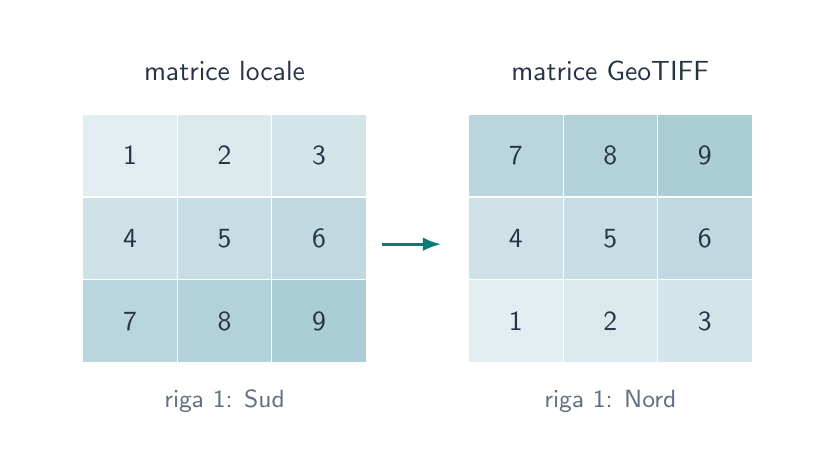
\begin{tikzpicture}[x=1cm,y=1cm]
\path[use as bounding box](-.1,-.15) rectangle(9.7,5.15);
\node[pLabel]at(2.4,4.6){matrice locale};
\filldraw[fill=GeoA!13,draw=white](0.6,3.0)rectangle(1.7999999999999998,4.05);
\node[pLabel]at(1.2,3.525){1};
\filldraw[fill=GeoA!16,draw=white](1.7999999999999998,3.0)rectangle(3.0,4.05);
\node[pLabel]at(2.4,3.525){2};
\filldraw[fill=GeoA!19,draw=white](3.0,3.0)rectangle(4.2,4.05);
\node[pLabel]at(3.6,3.525){3};
\filldraw[fill=GeoA!22,draw=white](0.6,1.9500000000000002)rectangle(1.7999999999999998,3.0);
\node[pLabel]at(1.2,2.475){4};
\filldraw[fill=GeoA!25,draw=white](1.7999999999999998,1.9500000000000002)rectangle(3.0,3.0);
\node[pLabel]at(2.4,2.475){5};
\filldraw[fill=GeoA!28,draw=white](3.0,1.9500000000000002)rectangle(4.2,3.0);
\node[pLabel]at(3.6,2.475){6};
\filldraw[fill=GeoA!31,draw=white](0.6,0.9)rectangle(1.7999999999999998,1.9500000000000002);
\node[pLabel]at(1.2,1.425){7};
\filldraw[fill=GeoA!34,draw=white](1.7999999999999998,0.9)rectangle(3.0,1.9500000000000002);
\node[pLabel]at(2.4,1.425){8};
\filldraw[fill=GeoA!37,draw=white](3.0,0.9)rectangle(4.2,1.9500000000000002);
\node[pLabel]at(3.6,1.425){9};
\node[pNote]at(2.4,.4){riga 1: Sud};
\node[pLabel]at(7.3,4.6){matrice GeoTIFF};
\filldraw[fill=GeoA!31,draw=white](5.5,3.0)rectangle(6.7,4.05);
\node[pLabel]at(6.1,3.525){7};
\filldraw[fill=GeoA!34,draw=white](6.7,3.0)rectangle(7.9,4.05);
\node[pLabel]at(7.3,3.525){8};
\filldraw[fill=GeoA!37,draw=white](7.9,3.0)rectangle(9.1,4.05);
\node[pLabel]at(8.5,3.525){9};
\filldraw[fill=GeoA!22,draw=white](5.5,1.9500000000000002)rectangle(6.7,3.0);
\node[pLabel]at(6.1,2.475){4};
\filldraw[fill=GeoA!25,draw=white](6.7,1.9500000000000002)rectangle(7.9,3.0);
\node[pLabel]at(7.3,2.475){5};
\filldraw[fill=GeoA!28,draw=white](7.9,1.9500000000000002)rectangle(9.1,3.0);
\node[pLabel]at(8.5,2.475){6};
\filldraw[fill=GeoA!13,draw=white](5.5,0.9)rectangle(6.7,1.9500000000000002);
\node[pLabel]at(6.1,1.425){1};
\filldraw[fill=GeoA!16,draw=white](6.7,0.9)rectangle(7.9,1.9500000000000002);
\node[pLabel]at(7.3,1.425){2};
\filldraw[fill=GeoA!19,draw=white](7.9,0.9)rectangle(9.1,1.9500000000000002);
\node[pLabel]at(8.5,1.425){3};
\node[pNote]at(7.3,.4){riga 1: Nord};
\draw[pEdge](4.4,2.4)--(5.15,2.4);
\end{tikzpicture}

\end{minipage}\end{lrbox}
\typeout{FULLBOX:011:PilotLeftBox:\the\ht\PilotLeftBox:\the\dp\PilotLeftBox}

\begin{lrbox}{\PilotRightBox}
\begin{minipage}[t]{7.55cm}\raggedright\color{Ink}\fontsize{11.3}{14.8}\selectfont
\PBody{La prima riga della matrice locale rappresenta il margine Sud. La prima riga restituita dal GeoTIFF rappresenta il margine Nord.}
\vspace{2.5mm}
\PInfo{Il diagramma mostra l’ordine degli elementi in memoria. Per confrontare le quote occorre invertire le righe di una delle due matrici.}
\PCode{R · confrontare lo stesso ordine}{011_esempio.R}
\end{minipage}\end{lrbox}
\typeout{FULLBOX:011:PilotRightBox:\the\ht\PilotRightBox:\the\dp\PilotRightBox}

\begin{tikzpicture}[remember picture,overlay]
\PilotChrome{Invertire le righe cambia l’orientamento}{II · GEOMETRIA RASTER}{11}{Media e istogramma non riconoscono l’inversione Nord–Sud: occorrono celle di posizione nota.}
\node[anchor=north west,inner sep=0] at([xshift=.96cm,yshift=-2.13cm]current page.north west){\usebox{\PilotLeftBox}};
\node[anchor=north west,inner sep=0] at([xshift=11.52cm,yshift=-2.13cm]current page.north west){\usebox{\PilotRightBox}};
\node[anchor=north east,inner sep=0] at([xshift=17.65cm,yshift=-12.06cm]current page.north west){\color{Classical}\fontsize{7.7}{9.2}\selectfont\href{../../03_Notebook_svolti/M12_Tessera/M12_N02.html}{M12\_N02 · notebook svolto}};
\end{tikzpicture}\end{frame}

\begin{frame}[plain]\hypertarget{slide12}{}
\bookmark[level=1,page=12]{Una griglia completa richiede celle uniche}
\begin{lrbox}{\TitleBox}
\begin{minipage}[t]{17.7cm}\raggedright\color{Ink}\fontsize{11.3}{14.8}\selectfont
\color{Navy}\bfseries\fontsize{20.6}{24.5}\selectfont Una griglia completa richiede celle uniche
\end{minipage}\end{lrbox}
\typeout{FULLBOX:012:TitleBox:\the\ht\TitleBox:\the\dp\TitleBox}

\begin{lrbox}{\RecallBox}
\begin{minipage}[t]{14.3cm}\raggedright\color{Ink}\fontsize{11.3}{14.8}\selectfont
\fontsize{10.3}{13.8}\selectfont La struttura della griglia va verificata prima di trasformare una colonna di valori in una matrice.
\end{minipage}\end{lrbox}
\typeout{FULLBOX:012:RecallBox:\the\ht\RecallBox:\the\dp\RecallBox}

\begin{lrbox}{\PilotLeftBox}
\begin{minipage}[t]{10.05cm}\raggedright\color{Ink}\fontsize{11.3}{14.8}\selectfont
{\fontsize{10.2}{13.1}\selectfont\renewcommand{\arraystretch}{1.45}\begin{tabular}{@{}p{4.3cm}p{4.7cm}@{}}\toprule
\textbf{Controllo} & \textbf{Problema riconosciuto}\\\midrule
Coppia riga–colonna unica & Duplicato della stessa cella\\
24 × 30 coppie attese & Cella assente nella tabella\\
Passo di 30 m su ogni asse & Coordinate irregolari\\
Ordinamento esplicito & Riempimento della matrice errato\\
Mancanti conservati & Scorrimento dei valori successivi\\
\bottomrule\end{tabular}}

\end{minipage}\end{lrbox}
\typeout{FULLBOX:012:PilotLeftBox:\the\ht\PilotLeftBox:\the\dp\PilotLeftBox}

\begin{lrbox}{\PilotRightBox}
\begin{minipage}[t]{7.55cm}\raggedright\color{Ink}\fontsize{11.3}{14.8}\selectfont
\PBody{Una riga assente e una riga presente con valore mancante non hanno lo stesso effetto sulla ricostruzione della matrice.}
\vspace{2.5mm}
\PInfo{Il controllo delle chiavi viene prima di matrix(). Un ordinamento plausibile non basta a garantire che ogni valore occupi la propria cella.}
\PBody{Per questo caso rettangolare confrontiamo la tabella con tutte le combinazioni ammesse di riga e colonna.}
\vspace{2.5mm}

\end{minipage}\end{lrbox}
\typeout{FULLBOX:012:PilotRightBox:\the\ht\PilotRightBox:\the\dp\PilotRightBox}

\begin{tikzpicture}[remember picture,overlay]
\PilotChrome{Una griglia completa richiede celle uniche}{II · GEOMETRIA RASTER}{12}{La struttura della griglia va verificata prima di trasformare una colonna di valori in una matrice.}
\node[anchor=north west,inner sep=0] at([xshift=.96cm,yshift=-2.13cm]current page.north west){\usebox{\PilotLeftBox}};
\node[anchor=north west,inner sep=0] at([xshift=11.52cm,yshift=-2.13cm]current page.north west){\usebox{\PilotRightBox}};
\node[anchor=north east,inner sep=0] at([xshift=17.65cm,yshift=-12.06cm]current page.north west){\color{Classical}\fontsize{7.7}{9.2}\selectfont\href{../../03_Notebook_svolti/M12_Tessera/M12_N01.html}{M12\_N01 · notebook svolto}};
\end{tikzpicture}\end{frame}

\begin{frame}[plain]\hypertarget{slide13}{}
\bookmark[level=1,page=13]{L’ordinamento rende riproducibile la ricostruzione}
\begin{lrbox}{\TitleBox}
\begin{minipage}[t]{17.7cm}\raggedright\color{Ink}\fontsize{11.3}{14.8}\selectfont
\color{Navy}\bfseries\fontsize{20.6}{24.5}\selectfont L’ordinamento rende riproducibile la ricostruzione
\end{minipage}\end{lrbox}
\typeout{FULLBOX:013:TitleBox:\the\ht\TitleBox:\the\dp\TitleBox}

\begin{lrbox}{\RecallBox}
\begin{minipage}[t]{14.3cm}\raggedright\color{Ink}\fontsize{11.3}{14.8}\selectfont
\fontsize{10.3}{13.8}\selectfont La stessa procedura deve ricostruire la griglia anche se l’ordine iniziale delle righe cambia.
\end{minipage}\end{lrbox}
\typeout{FULLBOX:013:RecallBox:\the\ht\RecallBox:\the\dp\RecallBox}

\begin{lrbox}{\PilotLeftBox}
\begin{minipage}[t]{10.05cm}\raggedright\color{Ink}\fontsize{11.3}{14.8}\selectfont
\[Z_{i+1,j+1}=z_{ij},\quad i=0,\ldots,23,\quad j=0,\ldots,29\]
\PInfo{Gli indici del file partono da zero; quelli della matrice R partono da uno. La corrispondenza esplicita evita uno spostamento di una cella.}

\end{minipage}\end{lrbox}
\typeout{FULLBOX:013:PilotLeftBox:\the\ht\PilotLeftBox:\the\dp\PilotLeftBox}

\begin{lrbox}{\PilotRightBox}
\begin{minipage}[t]{7.55cm}\raggedright\color{Ink}\fontsize{11.3}{14.8}\selectfont
\PBody{Ordiniamo prima le righe della tabella. Il riempimento per righe segue poi la convenzione locale da Sud verso Nord.}
\vspace{2.5mm}
\PSmall{La proprietà byrow=TRUE deve essere letta insieme all’ordinamento del file.}
\PCode{R · ricostruire e controllare}{013_esempio.R}
\end{minipage}\end{lrbox}
\typeout{FULLBOX:013:PilotRightBox:\the\ht\PilotRightBox:\the\dp\PilotRightBox}

\begin{tikzpicture}[remember picture,overlay]
\PilotChrome{L’ordinamento rende riproducibile la ricostruzione}{II · GEOMETRIA RASTER}{13}{La stessa procedura deve ricostruire la griglia anche se l’ordine iniziale delle righe cambia.}
\node[anchor=north west,inner sep=0] at([xshift=.96cm,yshift=-2.13cm]current page.north west){\usebox{\PilotLeftBox}};
\node[anchor=north west,inner sep=0] at([xshift=11.52cm,yshift=-2.13cm]current page.north west){\usebox{\PilotRightBox}};
\node[anchor=north east,inner sep=0] at([xshift=17.65cm,yshift=-12.06cm]current page.north west){\color{Classical}\fontsize{7.7}{9.2}\selectfont\href{../../03_Notebook_svolti/M12_Tessera/M12_N01.html}{M12\_N01 · notebook svolto}};
\end{tikzpicture}\end{frame}

\begin{frame}[plain]\hypertarget{slide14}{}
\bookmark[level=1,page=14]{Un’inversione conserva l’istogramma}
\begin{lrbox}{\TitleBox}
\begin{minipage}[t]{17.7cm}\raggedright\color{Ink}\fontsize{11.3}{14.8}\selectfont
\color{Navy}\bfseries\fontsize{20.6}{24.5}\selectfont Un’inversione conserva l’istogramma
\end{minipage}\end{lrbox}
\typeout{FULLBOX:014:TitleBox:\the\ht\TitleBox:\the\dp\TitleBox}

\begin{lrbox}{\RecallBox}
\begin{minipage}[t]{14.3cm}\raggedright\color{Ink}\fontsize{11.3}{14.8}\selectfont
\fontsize{10.3}{13.8}\selectfont La plausibilità visiva acquista valore quando è accompagnata da corrispondenze verificabili.
\end{minipage}\end{lrbox}
\typeout{FULLBOX:014:RecallBox:\the\ht\RecallBox:\the\dp\RecallBox}

\begin{lrbox}{\FullWideBox}
\begin{minipage}[t]{18.1cm}\raggedright\color{Ink}\fontsize{11.3}{14.8}\selectfont
\centering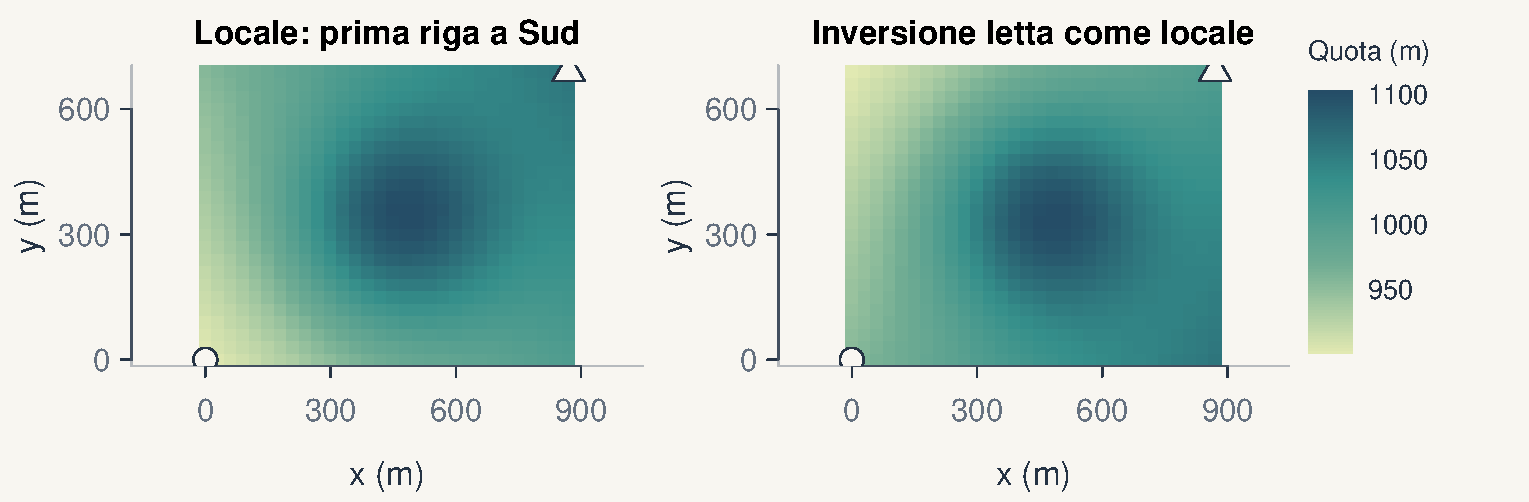
\includegraphics[width=18.05cm,height=5.8cm,keepaspectratio]{Risultati/Figure/02_orientamento.pdf}
\end{minipage}\end{lrbox}
\typeout{FULLBOX:014:FullWideBox:\the\ht\FullWideBox:\the\dp\FullWideBox}

\begin{lrbox}{\PilotRightBox}
\begin{minipage}[t]{18.1cm}\raggedright\color{Ink}\fontsize{11.3}{14.8}\selectfont
\PBody{Gli stessi valori sono rappresentati con due ordinamenti: a sinistra la convenzione locale corretta, a destra l’inversione delle righe interpretata erroneamente come locale. Media e distribuzione restano uguali. Il confronto delle celle di posizione nota riconosce l’errore geografico.}
\end{minipage}\end{lrbox}
\typeout{FULLBOX:014:PilotRightBox:\the\ht\PilotRightBox:\the\dp\PilotRightBox}

\begin{tikzpicture}[remember picture,overlay]
\PilotChrome{Un’inversione conserva l’istogramma}{II · GEOMETRIA RASTER}{14}{La plausibilità visiva acquista valore quando è accompagnata da corrispondenze verificabili.}
\node[anchor=north west,inner sep=0] at([xshift=.96cm,yshift=-2.13cm]current page.north west){\usebox{\FullWideBox}};
\node[anchor=north west,inner sep=0] at([xshift=.96cm,yshift=-8.25cm]current page.north west){\usebox{\PilotRightBox}};
\node[anchor=north east,inner sep=0] at([xshift=17.65cm,yshift=-12.06cm]current page.north west){\color{Classical}\fontsize{7.7}{9.2}\selectfont\href{../../03_Notebook_svolti/M12_Tessera/M12_N02.html}{M12\_N02 · notebook svolto}};
\end{tikzpicture}\end{frame}

\begin{frame}[plain]\hypertarget{slide15}{}
\bookmark[level=1,page=15]{Un riferimento assegnato non sposta le celle}
\begin{lrbox}{\TitleBox}
\begin{minipage}[t]{17.7cm}\raggedright\color{Ink}\fontsize{11.3}{14.8}\selectfont
\color{Navy}\bfseries\fontsize{20.6}{24.5}\selectfont Un riferimento assegnato non sposta le celle
\end{minipage}\end{lrbox}
\typeout{FULLBOX:015:TitleBox:\the\ht\TitleBox:\the\dp\TitleBox}

\begin{lrbox}{\RecallBox}
\begin{minipage}[t]{14.3cm}\raggedright\color{Ink}\fontsize{11.3}{14.8}\selectfont
\fontsize{10.3}{13.8}\selectfont Un codice EPSG comune è necessario in molte operazioni, ma non garantisce la coincidenza delle celle.
\end{minipage}\end{lrbox}
\typeout{FULLBOX:015:RecallBox:\the\ht\RecallBox:\the\dp\RecallBox}

\begin{lrbox}{\PilotLeftBox}
\begin{minipage}[t]{10.05cm}\raggedright\color{Ink}\fontsize{11.3}{14.8}\selectfont
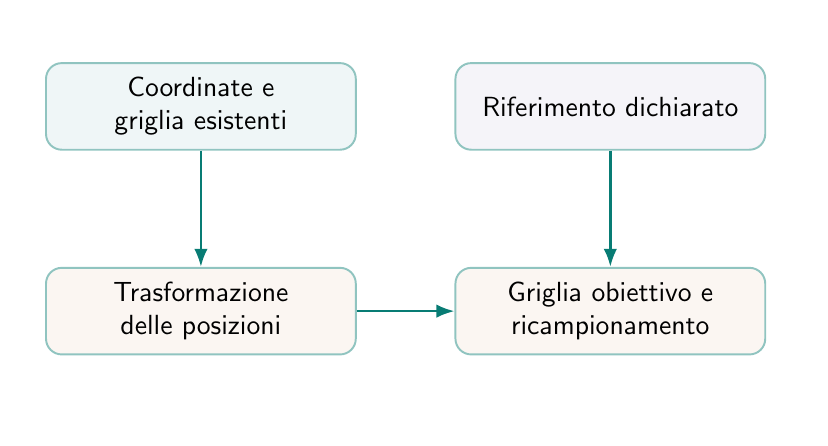
\begin{tikzpicture}[x=1cm,y=1cm]
\path[use as bounding box](-.1,-.15) rectangle(9.7,4.8);
\node[pFlow,text width=3.7cm,fill=GeoA!7] (a) at(2.1,3.8){Coordinate e griglia esistenti};
\node[pFlow,text width=3.7cm,fill=GeoC!7] (b) at(7.3,3.8){Riferimento dichiarato};
\node[pFlow,text width=3.7cm,fill=GeoB!7] (c) at(2.1,1.2){Trasformazione delle posizioni};
\node[pFlow,text width=3.7cm,fill=GeoB!7] (d) at(7.3,1.2){Griglia obiettivo e ricampionamento};
\draw[pEdge] (a) -- (c);
\draw[pEdge] (b) -- (d);
\draw[pEdge] (c) -- (d);
\end{tikzpicture}

\end{minipage}\end{lrbox}
\typeout{FULLBOX:015:PilotLeftBox:\the\ht\PilotLeftBox:\the\dp\PilotLeftBox}

\begin{lrbox}{\PilotRightBox}
\begin{minipage}[t]{7.55cm}\raggedright\color{Ink}\fontsize{11.3}{14.8}\selectfont
\PBody{Assegnare un CRS descrive l’interpretazione delle coordinate già presenti. Una riproiezione richiede invece di trasformare le posizioni e scegliere la griglia di uscita.}
\vspace{2.5mm}
\PInfo{Il GeoTIFF del corso possiede già un riferimento UTM fittizio. Non lo usiamo come prova che il terreno rappresenti una località reale.}
\PBody{Per combinare raster servono anche estensione, origine, risoluzione e allineamento compatibili.}
\vspace{2.5mm}

\end{minipage}\end{lrbox}
\typeout{FULLBOX:015:PilotRightBox:\the\ht\PilotRightBox:\the\dp\PilotRightBox}

\begin{tikzpicture}[remember picture,overlay]
\PilotChrome{Un riferimento assegnato non sposta le celle}{II · GEOMETRIA RASTER}{15}{Un codice EPSG comune è necessario in molte operazioni, ma non garantisce la coincidenza delle celle.}
\node[anchor=north west,inner sep=0] at([xshift=.96cm,yshift=-2.13cm]current page.north west){\usebox{\PilotLeftBox}};
\node[anchor=north west,inner sep=0] at([xshift=11.52cm,yshift=-2.13cm]current page.north west){\usebox{\PilotRightBox}};
\node[anchor=north east,inner sep=0] at([xshift=17.65cm,yshift=-12.06cm]current page.north west){\color{Classical}\fontsize{7.7}{9.2}\selectfont\href{../../03_Notebook_svolti/M12_Tessera/M12_N03.html}{M12\_N03 · notebook svolto}};
\end{tikzpicture}\end{frame}

\begin{frame}[plain]\hypertarget{slide16}{}
\bookmark[level=1,page=16]{Leggere il GeoTIFF conserva i metadati}
\begin{lrbox}{\TitleBox}
\begin{minipage}[t]{17.7cm}\raggedright\color{Ink}\fontsize{11.3}{14.8}\selectfont
\color{Navy}\bfseries\fontsize{20.6}{24.5}\selectfont Leggere il GeoTIFF conserva i metadati
\end{minipage}\end{lrbox}
\typeout{FULLBOX:016:TitleBox:\the\ht\TitleBox:\the\dp\TitleBox}

\begin{lrbox}{\RecallBox}
\begin{minipage}[t]{14.3cm}\raggedright\color{Ink}\fontsize{11.3}{14.8}\selectfont
\fontsize{10.3}{13.8}\selectfont Un file leggibile deve ancora essere confrontato con le caratteristiche attese.
\end{minipage}\end{lrbox}
\typeout{FULLBOX:016:RecallBox:\the\ht\RecallBox:\the\dp\RecallBox}

\begin{lrbox}{\PilotLeftBox}
\begin{minipage}[t]{10.05cm}\raggedright\color{Ink}\fontsize{11.3}{14.8}\selectfont
{\fontsize{10.2}{13.1}\selectfont\renewcommand{\arraystretch}{1.45}\begin{tabular}{@{}p{3.4cm}p{5.6cm}@{}}\toprule
\textbf{Proprietà} & \textbf{Che cosa verificare}\\\midrule
CRS & Riferimento e unità metriche\\
Risoluzione & Passo di 30 m sui due assi\\
Estensione & Bordi esterni convenzionali\\
Tipo numerico & Precisione delle quote\\
NoData & Codice distinto dai valori validi\\
\bottomrule\end{tabular}}

\end{minipage}\end{lrbox}
\typeout{FULLBOX:016:PilotLeftBox:\the\ht\PilotLeftBox:\the\dp\PilotLeftBox}

\begin{lrbox}{\PilotRightBox}
\begin{minipage}[t]{7.55cm}\raggedright\color{Ink}\fontsize{11.3}{14.8}\selectfont
\PBody{terra restituisce un oggetto SpatRaster che collega valori e geometria. L’apertura del file non richiede necessariamente di caricare tutti i valori in memoria.}
\vspace{2.5mm}
\PInfo{Il percorso è locale. Il pacchetto include il GeoTIFF originale e ne documenta la natura sintetica.}
\PCode{R · leggere dati e riferimento}{016_esempio.R}
\end{minipage}\end{lrbox}
\typeout{FULLBOX:016:PilotRightBox:\the\ht\PilotRightBox:\the\dp\PilotRightBox}

\begin{tikzpicture}[remember picture,overlay]
\PilotChrome{Leggere il GeoTIFF conserva i metadati}{II · GEOMETRIA RASTER}{16}{Un file leggibile deve ancora essere confrontato con le caratteristiche attese.}
\node[anchor=north west,inner sep=0] at([xshift=.96cm,yshift=-2.13cm]current page.north west){\usebox{\PilotLeftBox}};
\node[anchor=north west,inner sep=0] at([xshift=11.52cm,yshift=-2.13cm]current page.north west){\usebox{\PilotRightBox}};
\node[anchor=north east,inner sep=0] at([xshift=17.65cm,yshift=-12.06cm]current page.north west){\color{Classical}\fontsize{7.7}{9.2}\selectfont\href{../../03_Notebook_svolti/M12_Tessera/M12_N03.html}{M12\_N03 · notebook svolto}};
\end{tikzpicture}\end{frame}

\begin{frame}[plain]\hypertarget{slide17}{}
\bookmark[level=1,page=17]{Collegare coordinate locali e GeoTIFF}
\begin{lrbox}{\TitleBox}
\begin{minipage}[t]{17.7cm}\raggedright\color{Ink}\fontsize{11.3}{14.8}\selectfont
\color{Navy}\bfseries\fontsize{20.6}{24.5}\selectfont Collegare coordinate locali e GeoTIFF
\end{minipage}\end{lrbox}
\typeout{FULLBOX:017:TitleBox:\the\ht\TitleBox:\the\dp\TitleBox}

\begin{lrbox}{\RecallBox}
\begin{minipage}[t]{14.3cm}\raggedright\color{Ink}\fontsize{11.3}{14.8}\selectfont
\fontsize{10.3}{13.8}\selectfont La conversione fra griglia locale e file georeferenziato deve conservare le posizioni dei centri.
\end{minipage}\end{lrbox}
\typeout{FULLBOX:017:RecallBox:\the\ht\RecallBox:\the\dp\RecallBox}

\begin{lrbox}{\PilotLeftBox}
\begin{minipage}[t]{10.05cm}\raggedright\color{Ink}\fontsize{11.3}{14.8}\selectfont
\[E=x_{\mathrm{locale}}+500015\]
\[N=y_{\mathrm{locale}}+4999295\]
\PInfo{Questa relazione riguarda i centri delle celle del dataset sintetico. È una traslazione convenzionale, non una proiezione di coordinate geografiche.}

\end{minipage}\end{lrbox}
\typeout{FULLBOX:017:PilotLeftBox:\the\ht\PilotLeftBox:\the\dp\PilotLeftBox}

\begin{lrbox}{\PilotRightBox}
\begin{minipage}[t]{7.55cm}\raggedright\color{Ink}\fontsize{11.3}{14.8}\selectfont
\PBody{Il centro locale $(0,0)$ m corrisponde alla cella Sud-Ovest del GeoTIFF. Il centro locale $(870,690)$ m corrisponde alla cella Nord-Est.}
\vspace{2.5mm}
\PBody{La relazione è ricavata dai bordi del file e dal mezzo passo. Verrà riutilizzata per esportare le celle interne senza traslarle.}
\vspace{2.5mm}

\end{minipage}\end{lrbox}
\typeout{FULLBOX:017:PilotRightBox:\the\ht\PilotRightBox:\the\dp\PilotRightBox}

\begin{tikzpicture}[remember picture,overlay]
\PilotChrome{Collegare coordinate locali e GeoTIFF}{II · GEOMETRIA RASTER}{17}{La conversione fra griglia locale e file georeferenziato deve conservare le posizioni dei centri.}
\node[anchor=north west,inner sep=0] at([xshift=.96cm,yshift=-2.13cm]current page.north west){\usebox{\PilotLeftBox}};
\node[anchor=north west,inner sep=0] at([xshift=11.52cm,yshift=-2.13cm]current page.north west){\usebox{\PilotRightBox}};
\node[anchor=north east,inner sep=0] at([xshift=17.65cm,yshift=-12.06cm]current page.north west){\color{Classical}\fontsize{7.7}{9.2}\selectfont\href{../../03_Notebook_svolti/M12_Tessera/M12_N03.html}{M12\_N03 · notebook svolto}};
\end{tikzpicture}\end{frame}

\begin{frame}[plain]\hypertarget{slide18}{}
\bookmark[level=1,page=18]{Pixel e supporto della misura}
\begin{lrbox}{\TitleBox}
\begin{minipage}[t]{17.7cm}\raggedright\color{Ink}\fontsize{11.3}{14.8}\selectfont
\color{Navy}\bfseries\fontsize{20.6}{24.5}\selectfont Pixel e supporto della misura
\end{minipage}\end{lrbox}
\typeout{FULLBOX:018:TitleBox:\the\ht\TitleBox:\the\dp\TitleBox}

\begin{lrbox}{\RecallBox}
\begin{minipage}[t]{14.3cm}\raggedright\color{Ink}\fontsize{11.3}{14.8}\selectfont
\fontsize{10.3}{13.8}\selectfont Per confrontare prodotti diversi servono il significato dei valori e la loro scala di rappresentazione.
\end{minipage}\end{lrbox}
\typeout{FULLBOX:018:RecallBox:\the\ht\RecallBox:\the\dp\RecallBox}

\begin{lrbox}{\PilotLeftBox}
\begin{minipage}[t]{10.05cm}\raggedright\color{Ink}\fontsize{11.3}{14.8}\selectfont
{\fontsize{10.2}{13.1}\selectfont\renewcommand{\arraystretch}{1.45}\begin{tabular}{@{}p{4.2cm}p{4.8cm}@{}}\toprule
\textbf{Valore nella cella} & \textbf{Interpretazione possibile}\\\midrule
Quota di un DEM & Stima della superficie a una posizione\\
Riflettanza & Segnale riferito al supporto del sensore\\
Classe litologica & Categoria assegnata alla cella\\
Media di quattro celle & Sintesi su un supporto più grande\\
\bottomrule\end{tabular}}

\end{minipage}\end{lrbox}
\typeout{FULLBOX:018:PilotLeftBox:\the\ht\PilotLeftBox:\the\dp\PilotLeftBox}

\begin{lrbox}{\PilotRightBox}
\begin{minipage}[t]{7.55cm}\raggedright\color{Ink}\fontsize{11.3}{14.8}\selectfont
\PBody{La cella è una parte della geometria raster. Il supporto fisico o statistico del valore dipende da come il prodotto è stato ottenuto.}
\vspace{2.5mm}
\PInfo{Nel caso guida le quote sono sintetiche e associate ai centri. L’aggregazione produce una media dei valori: non la confondiamo con una nuova misura sul terreno.}
\PBody{Pixel più piccoli e sensori con maggiore capacità di risolvere dettagli sono proprietà da documentare separatamente.}
\vspace{2.5mm}

\end{minipage}\end{lrbox}
\typeout{FULLBOX:018:PilotRightBox:\the\ht\PilotRightBox:\the\dp\PilotRightBox}

\begin{tikzpicture}[remember picture,overlay]
\PilotChrome{Pixel e supporto della misura}{II · GEOMETRIA RASTER}{18}{Per confrontare prodotti diversi servono il significato dei valori e la loro scala di rappresentazione.}
\node[anchor=north west,inner sep=0] at([xshift=.96cm,yshift=-2.13cm]current page.north west){\usebox{\PilotLeftBox}};
\node[anchor=north west,inner sep=0] at([xshift=11.52cm,yshift=-2.13cm]current page.north west){\usebox{\PilotRightBox}};
\end{tikzpicture}\end{frame}

\begin{frame}[plain]\hypertarget{slide19}{}
\bookmark[level=1,page=19]{Laboratorio: rendere riconoscibile ogni cella}
\begin{lrbox}{\TitleBox}
\begin{minipage}[t]{17.7cm}\raggedright\color{Ink}\fontsize{11.3}{14.8}\selectfont
\color{Navy}\bfseries\fontsize{20.6}{24.5}\selectfont Laboratorio: rendere riconoscibile ogni cella
\end{minipage}\end{lrbox}
\typeout{FULLBOX:019:TitleBox:\the\ht\TitleBox:\the\dp\TitleBox}

\begin{lrbox}{\RecallBox}
\begin{minipage}[t]{14.3cm}\raggedright\color{Ink}\fontsize{11.3}{14.8}\selectfont
\fontsize{10.3}{13.8}\selectfont Il controllo iniziale della geometria protegge tutte le elaborazioni successive.
\end{minipage}\end{lrbox}
\typeout{FULLBOX:019:RecallBox:\the\ht\RecallBox:\the\dp\RecallBox}

\begin{lrbox}{\PilotLeftBox}
\begin{minipage}[t]{10.05cm}\raggedright\color{Ink}\fontsize{11.3}{14.8}\selectfont
\PLab{https://marzione00.github.io/Lab_Geo/\#laboratorio/m12-griglia}{Esperimento online · geometria raster}
{\fontsize{10.2}{13.1}\selectfont\renewcommand{\arraystretch}{1.45}\begin{tabular}{@{}p{4.2cm}p{4.8cm}@{}}\toprule
\textbf{Attività} & \textbf{Risultato da conservare}\\\midrule
N01: audit & 720 coppie uniche, passo regolare\\
N02: orientamento & Confronto dei quattro angoli\\
N03: GeoTIFF & Dimensioni, CRS, estensione e risoluzione\\
Corrispondenza & Centri locali e centri georeferenziati\\
Conclusione & Natura sintetica e convenzioni esplicite\\
\bottomrule\end{tabular}}

\end{minipage}\end{lrbox}
\typeout{FULLBOX:019:PilotLeftBox:\the\ht\PilotLeftBox:\the\dp\PilotLeftBox}

\begin{lrbox}{\PilotRightBox}
\begin{minipage}[t]{7.55cm}\raggedright\color{Ink}\fontsize{11.3}{14.8}\selectfont
\PBody{Il primo prodotto del modulo è una scheda della griglia. Deve permettere a un’altra persona di ricostruire dove si trova ciascun valore.}
\vspace{2.5mm}
\PInfo{Se il controllo degli angoli fallisce, fermiamo la catena di elaborazione: pendenze, indici e sintesi erediteranno la geometria errata.}
\PBody{Passiamo ora alle celle escluse e al dominio effettivamente descritto.}
\vspace{2.5mm}

\end{minipage}\end{lrbox}
\typeout{FULLBOX:019:PilotRightBox:\the\ht\PilotRightBox:\the\dp\PilotRightBox}

\begin{tikzpicture}[remember picture,overlay]
\PilotChrome{Laboratorio: rendere riconoscibile ogni cella}{II · GEOMETRIA RASTER}{19}{Il controllo iniziale della geometria protegge tutte le elaborazioni successive.}
\node[anchor=north west,inner sep=0] at([xshift=.96cm,yshift=-2.13cm]current page.north west){\usebox{\PilotLeftBox}};
\node[anchor=north west,inner sep=0] at([xshift=11.52cm,yshift=-2.13cm]current page.north west){\usebox{\PilotRightBox}};
\node[anchor=north east,inner sep=0] at([xshift=17.65cm,yshift=-12.06cm]current page.north west){\color{Classical}\fontsize{7.7}{9.2}\selectfont\href{../../03_Notebook_svolti/M12_Tessera/M12_N03.html}{M12\_N03 · notebook svolto}};
\end{tikzpicture}\end{frame}

\begin{frame}[plain]\hypertarget{slide20}{}
\bookmark[level=0,page=20]{III · MASCHERE E DOMINIO}
\bookmark[level=1,page=20]{La maschera definisce il dominio disponibile}
\begin{lrbox}{\TitleBox}
\begin{minipage}[t]{17.7cm}\raggedright\color{Ink}\fontsize{11.3}{14.8}\selectfont
\color{Navy}\bfseries\fontsize{20.6}{24.5}\selectfont La maschera definisce il dominio disponibile
\end{minipage}\end{lrbox}
\typeout{FULLBOX:020:TitleBox:\the\ht\TitleBox:\the\dp\TitleBox}

\begin{lrbox}{\RecallBox}
\begin{minipage}[t]{14.3cm}\raggedright\color{Ink}\fontsize{11.3}{14.8}\selectfont
\fontsize{10.3}{13.8}\selectfont La maschera appartiene al dato e condiziona l’interpretazione delle sue sintesi.
\end{minipage}\end{lrbox}
\typeout{FULLBOX:020:RecallBox:\the\ht\RecallBox:\the\dp\RecallBox}

\begin{lrbox}{\PilotLeftBox}
\begin{minipage}[t]{10.05cm}\raggedright\color{Ink}\fontsize{11.3}{14.8}\selectfont
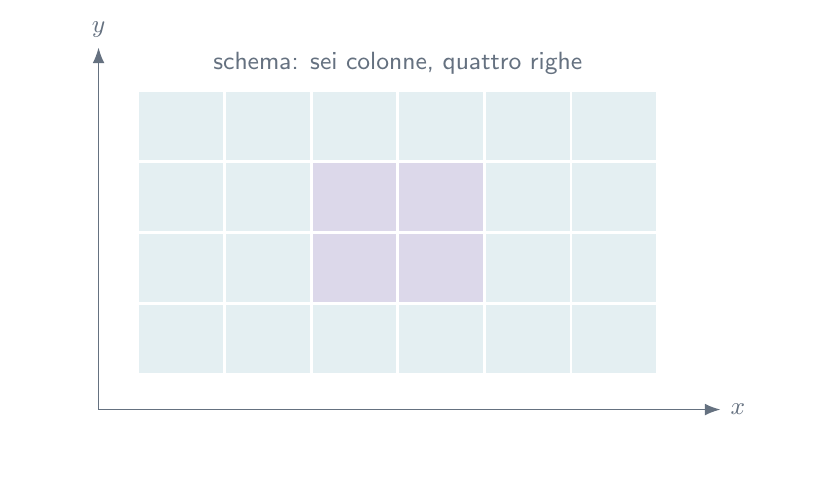
\begin{tikzpicture}[x=1cm,y=1cm]
\path[use as bounding box](-.1,-.15) rectangle(9.7,5.25);
\draw[pAxis](.8,.4)--(8.7,.4)node[right,pNote]{$x$};
\draw[pAxis](.8,.4)--(.8,5.0)node[above,pNote]{$y$};
\filldraw[fill=GeoA!12,draw=white,line width=1pt](1.3,0.85)rectangle(2.4000000000000004,1.75);
\filldraw[fill=GeoA!12,draw=white,line width=1pt](2.4000000000000004,0.85)rectangle(3.5000000000000004,1.75);
\filldraw[fill=GeoA!12,draw=white,line width=1pt](3.5,0.85)rectangle(4.6,1.75);
\filldraw[fill=GeoA!12,draw=white,line width=1pt](4.6000000000000005,0.85)rectangle(5.700000000000001,1.75);
\filldraw[fill=GeoA!12,draw=white,line width=1pt](5.7,0.85)rectangle(6.800000000000001,1.75);
\filldraw[fill=GeoA!12,draw=white,line width=1pt](6.8,0.85)rectangle(7.9,1.75);
\filldraw[fill=GeoA!12,draw=white,line width=1pt](1.3,1.75)rectangle(2.4000000000000004,2.65);
\filldraw[fill=GeoA!12,draw=white,line width=1pt](2.4000000000000004,1.75)rectangle(3.5000000000000004,2.65);
\filldraw[fill=GeoC!25,draw=white,line width=1pt](3.5,1.75)rectangle(4.6,2.65);
\filldraw[fill=GeoC!25,draw=white,line width=1pt](4.6000000000000005,1.75)rectangle(5.700000000000001,2.65);
\filldraw[fill=GeoA!12,draw=white,line width=1pt](5.7,1.75)rectangle(6.800000000000001,2.65);
\filldraw[fill=GeoA!12,draw=white,line width=1pt](6.8,1.75)rectangle(7.9,2.65);
\filldraw[fill=GeoA!12,draw=white,line width=1pt](1.3,2.65)rectangle(2.4000000000000004,3.55);
\filldraw[fill=GeoA!12,draw=white,line width=1pt](2.4000000000000004,2.65)rectangle(3.5000000000000004,3.55);
\filldraw[fill=GeoC!25,draw=white,line width=1pt](3.5,2.65)rectangle(4.6,3.55);
\filldraw[fill=GeoC!25,draw=white,line width=1pt](4.6000000000000005,2.65)rectangle(5.700000000000001,3.55);
\filldraw[fill=GeoA!12,draw=white,line width=1pt](5.7,2.65)rectangle(6.800000000000001,3.55);
\filldraw[fill=GeoA!12,draw=white,line width=1pt](6.8,2.65)rectangle(7.9,3.55);
\filldraw[fill=GeoA!12,draw=white,line width=1pt](1.3,3.5500000000000003)rectangle(2.4000000000000004,4.45);
\filldraw[fill=GeoA!12,draw=white,line width=1pt](2.4000000000000004,3.5500000000000003)rectangle(3.5000000000000004,4.45);
\filldraw[fill=GeoA!12,draw=white,line width=1pt](3.5,3.5500000000000003)rectangle(4.6,4.45);
\filldraw[fill=GeoA!12,draw=white,line width=1pt](4.6000000000000005,3.5500000000000003)rectangle(5.700000000000001,4.45);
\filldraw[fill=GeoA!12,draw=white,line width=1pt](5.7,3.5500000000000003)rectangle(6.800000000000001,4.45);
\filldraw[fill=GeoA!12,draw=white,line width=1pt](6.8,3.5500000000000003)rectangle(7.9,4.45);
\node[pNote]at(4.6,4.8){schema: sei colonne, quattro righe};
\end{tikzpicture}
\[m_{ij}=\begin{cases}1&\text{cella valida}\\0&\text{cella esclusa}\end{cases}\]

\end{minipage}\end{lrbox}
\typeout{FULLBOX:020:PilotLeftBox:\the\ht\PilotLeftBox:\the\dp\PilotLeftBox}

\begin{lrbox}{\PilotRightBox}
\begin{minipage}[t]{7.55cm}\raggedright\color{Ink}\fontsize{11.3}{14.8}\selectfont
\PBody{Una maschera distingue le celle utilizzabili dalle altre. L’esclusione può dipendere da assenza di misura, qualità insufficiente o scelta del dominio.}
\vspace{2.5mm}
\PInfo{Conserviamo separatamente i valori e la loro validità. Il colore delle celle escluse deve essere riconoscibile senza confondersi con la scala delle quote.}
\PBody{Il motivo della mancanza può essere legato alla morfologia o al fenomeno studiato.}
\vspace{2.5mm}

\end{minipage}\end{lrbox}
\typeout{FULLBOX:020:PilotRightBox:\the\ht\PilotRightBox:\the\dp\PilotRightBox}

\begin{tikzpicture}[remember picture,overlay]
\PilotChrome{La maschera definisce il dominio disponibile}{III · MASCHERE E DOMINIO}{20}{La maschera appartiene al dato e condiziona l’interpretazione delle sue sintesi.}
\node[anchor=north west,inner sep=0] at([xshift=.96cm,yshift=-2.13cm]current page.north west){\usebox{\PilotLeftBox}};
\node[anchor=north west,inner sep=0] at([xshift=11.52cm,yshift=-2.13cm]current page.north west){\usebox{\PilotRightBox}};
\node[anchor=north east,inner sep=0] at([xshift=17.65cm,yshift=-12.06cm]current page.north west){\color{Classical}\fontsize{7.7}{9.2}\selectfont\href{../../03_Notebook_svolti/M12_Tessera/M12_N04.html}{M12\_N04 · notebook svolto}};
\end{tikzpicture}\end{frame}

\begin{frame}[plain]\hypertarget{slide21}{}
\bookmark[level=1,page=21]{NoData e quota zero hanno significati diversi}
\begin{lrbox}{\TitleBox}
\begin{minipage}[t]{17.7cm}\raggedright\color{Ink}\fontsize{11.3}{14.8}\selectfont
\color{Navy}\bfseries\fontsize{20.6}{24.5}\selectfont NoData e quota zero hanno significati diversi
\end{minipage}\end{lrbox}
\typeout{FULLBOX:021:TitleBox:\the\ht\TitleBox:\the\dp\TitleBox}

\begin{lrbox}{\RecallBox}
\begin{minipage}[t]{14.3cm}\raggedright\color{Ink}\fontsize{11.3}{14.8}\selectfont
\fontsize{10.3}{13.8}\selectfont La validità della cella deve essere verificata prima di interpretare il suo numero.
\end{minipage}\end{lrbox}
\typeout{FULLBOX:021:RecallBox:\the\ht\RecallBox:\the\dp\RecallBox}

\begin{lrbox}{\PilotLeftBox}
\begin{minipage}[t]{10.05cm}\raggedright\color{Ink}\fontsize{11.3}{14.8}\selectfont
{\fontsize{10.2}{13.1}\selectfont\renewcommand{\arraystretch}{1.45}\begin{tabular}{@{}p{4.0cm}p{5.0cm}@{}}\toprule
\textbf{Stato} & \textbf{Interpretazione}\\\midrule
Quota 0 m & Valore fisico valido nel riferimento verticale\\
NA in R & Valore mancante nel calcolo\\
NoData nel file & Codice riservato alla mancanza\\
Cella fuori dominio & Posizione esclusa dalla domanda\\
Valore non valido & Misura respinta secondo un criterio\\
\bottomrule\end{tabular}}

\end{minipage}\end{lrbox}
\typeout{FULLBOX:021:PilotLeftBox:\the\ht\PilotLeftBox:\the\dp\PilotLeftBox}

\begin{lrbox}{\PilotRightBox}
\begin{minipage}[t]{7.55cm}\raggedright\color{Ink}\fontsize{11.3}{14.8}\selectfont
\PBody{Il GeoTIFF originale dichiara il valore $-9999$ come NoData. terra lo interpreta come mancante, non come una quota da usare nelle medie.}
\vspace{2.5mm}
\PInfo{Una codifica mancante deve essere compatibile con l’intervallo dei valori validi. La stessa sentinella non è automaticamente adatta a ogni variabile.}
\PBody{Un terreno a quota zero può essere pianeggiante o inclinato: lo zero non indica assenza di informazione.}
\vspace{2.5mm}

\end{minipage}\end{lrbox}
\typeout{FULLBOX:021:PilotRightBox:\the\ht\PilotRightBox:\the\dp\PilotRightBox}

\begin{tikzpicture}[remember picture,overlay]
\PilotChrome{NoData e quota zero hanno significati diversi}{III · MASCHERE E DOMINIO}{21}{La validità della cella deve essere verificata prima di interpretare il suo numero.}
\node[anchor=north west,inner sep=0] at([xshift=.96cm,yshift=-2.13cm]current page.north west){\usebox{\PilotLeftBox}};
\node[anchor=north west,inner sep=0] at([xshift=11.52cm,yshift=-2.13cm]current page.north west){\usebox{\PilotRightBox}};
\node[anchor=north east,inner sep=0] at([xshift=17.65cm,yshift=-12.06cm]current page.north west){\color{Classical}\fontsize{7.7}{9.2}\selectfont\href{../../03_Notebook_svolti/M12_Tessera/M12_N04.html}{M12\_N04 · notebook svolto}};
\end{tikzpicture}\end{frame}

\begin{frame}[plain]\hypertarget{slide22}{}
\bookmark[level=1,page=22]{Ventiquattro celle escluse restano localizzabili}
\begin{lrbox}{\TitleBox}
\begin{minipage}[t]{17.7cm}\raggedright\color{Ink}\fontsize{11.3}{14.8}\selectfont
\color{Navy}\bfseries\fontsize{20.6}{24.5}\selectfont Ventiquattro celle escluse restano localizzabili
\end{minipage}\end{lrbox}
\typeout{FULLBOX:022:TitleBox:\the\ht\TitleBox:\the\dp\TitleBox}

\begin{lrbox}{\RecallBox}
\begin{minipage}[t]{14.3cm}\raggedright\color{Ink}\fontsize{11.3}{14.8}\selectfont
\fontsize{10.3}{13.8}\selectfont Conservare la posizione delle celle escluse evita che la maschera diventi un semplice conteggio.
\end{minipage}\end{lrbox}
\typeout{FULLBOX:022:RecallBox:\the\ht\RecallBox:\the\dp\RecallBox}

\begin{lrbox}{\PilotLeftBox}
\begin{minipage}[t]{10.05cm}\raggedright\color{Ink}\fontsize{11.3}{14.8}\selectfont
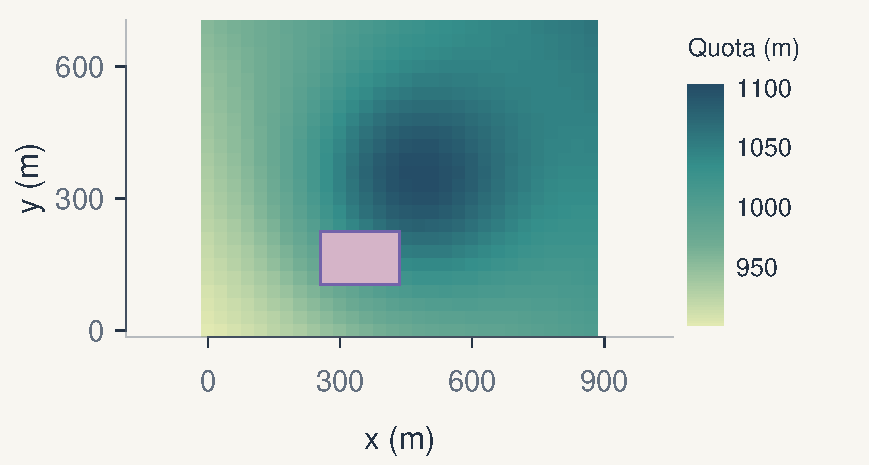
\includegraphics[width=9.85cm,height=5.25cm,keepaspectratio]{Risultati/Figure/04_maschera_nodata.pdf}
\vspace{1.5mm}
\PSmall{Finestra esclusa: indici originali riga 4–7 e colonna 9–14. La maschera contiene 24 celle.}

\end{minipage}\end{lrbox}
\typeout{FULLBOX:022:PilotLeftBox:\the\ht\PilotLeftBox:\the\dp\PilotLeftBox}

\begin{lrbox}{\PilotRightBox}
\begin{minipage}[t]{7.55cm}\raggedright\color{Ink}\fontsize{11.3}{14.8}\selectfont
\PBody{In R gli indici corrispondenti sono righe 5–8 e colonne 10–15. Il controllo del numero di celle rende esplicita la conversione.}
\vspace{2.5mm}
\PInfo{Le quote disponibili conservano la scala cromatica della carta iniziale. La mancanza è rappresentata con un colore separato.}
\PCode{R · maschera dichiarata}{022_esempio.R}
\end{minipage}\end{lrbox}
\typeout{FULLBOX:022:PilotRightBox:\the\ht\PilotRightBox:\the\dp\PilotRightBox}

\begin{tikzpicture}[remember picture,overlay]
\PilotChrome{Ventiquattro celle escluse restano localizzabili}{III · MASCHERE E DOMINIO}{22}{Conservare la posizione delle celle escluse evita che la maschera diventi un semplice conteggio.}
\node[anchor=north west,inner sep=0] at([xshift=.96cm,yshift=-2.13cm]current page.north west){\usebox{\PilotLeftBox}};
\node[anchor=north west,inner sep=0] at([xshift=11.52cm,yshift=-2.13cm]current page.north west){\usebox{\PilotRightBox}};
\node[anchor=north east,inner sep=0] at([xshift=17.65cm,yshift=-12.06cm]current page.north west){\color{Classical}\fontsize{7.7}{9.2}\selectfont\href{../../03_Notebook_svolti/M12_Tessera/M12_N04.html}{M12\_N04 · notebook svolto}};
\end{tikzpicture}\end{frame}

\begin{frame}[plain]\hypertarget{slide23}{}
\bookmark[level=1,page=23]{La copertura accompagna ogni media}
\begin{lrbox}{\TitleBox}
\begin{minipage}[t]{17.7cm}\raggedright\color{Ink}\fontsize{11.3}{14.8}\selectfont
\color{Navy}\bfseries\fontsize{20.6}{24.5}\selectfont La copertura accompagna ogni media
\end{minipage}\end{lrbox}
\typeout{FULLBOX:023:TitleBox:\the\ht\TitleBox:\the\dp\TitleBox}

\begin{lrbox}{\RecallBox}
\begin{minipage}[t]{14.3cm}\raggedright\color{Ink}\fontsize{11.3}{14.8}\selectfont
\fontsize{10.3}{13.8}\selectfont Numero di celle valide, loro posizione e causa di esclusione devono accompagnare il risultato.
\end{minipage}\end{lrbox}
\typeout{FULLBOX:023:RecallBox:\the\ht\RecallBox:\the\dp\RecallBox}

\begin{lrbox}{\PilotLeftBox}
\begin{minipage}[t]{10.05cm}\raggedright\color{Ink}\fontsize{11.3}{14.8}\selectfont
\[c=\frac{696}{720}\approx0{,}9667\]
\[\overline z_{\mathrm{disp}}=\frac{\sum_{ij}m_{ij}z_{ij}}{\sum_{ij}m_{ij}}\]
\PInfo{La notazione della somma si riferisce ai valori validi: nel codice selezioniamo esplicitamente le celle disponibili prima di calcolare la media.}

\end{minipage}\end{lrbox}
\typeout{FULLBOX:023:PilotLeftBox:\the\ht\PilotLeftBox:\the\dp\PilotLeftBox}

\begin{lrbox}{\PilotRightBox}
\begin{minipage}[t]{7.55cm}\raggedright\color{Ink}\fontsize{11.3}{14.8}\selectfont
\PBody{La media dei disponibili descrive le celle rimaste. Il suo trasferimento al dominio completo richiederebbe informazioni sul processo di mancanza.}
\vspace{2.5mm}
\PBody{La copertura del 96,67\% non dimostra che le celle osservate siano rappresentative della parte esclusa.}
\vspace{2.5mm}
\PSmall{Il dataset completo ci permette di confrontare le due medie come esperimento didattico.}

\end{minipage}\end{lrbox}
\typeout{FULLBOX:023:PilotRightBox:\the\ht\PilotRightBox:\the\dp\PilotRightBox}

\begin{tikzpicture}[remember picture,overlay]
\PilotChrome{La copertura accompagna ogni media}{III · MASCHERE E DOMINIO}{23}{Numero di celle valide, loro posizione e causa di esclusione devono accompagnare il risultato.}
\node[anchor=north west,inner sep=0] at([xshift=.96cm,yshift=-2.13cm]current page.north west){\usebox{\PilotLeftBox}};
\node[anchor=north west,inner sep=0] at([xshift=11.52cm,yshift=-2.13cm]current page.north west){\usebox{\PilotRightBox}};
\node[anchor=north east,inner sep=0] at([xshift=17.65cm,yshift=-12.06cm]current page.north west){\color{Classical}\fontsize{7.7}{9.2}\selectfont\href{../../03_Notebook_svolti/M12_Tessera/M12_N04.html}{M12\_N04 · notebook svolto}};
\end{tikzpicture}\end{frame}

\begin{frame}[plain]\hypertarget{slide24}{}
\bookmark[level=1,page=24]{Sostituire i mancanti con zero altera il risultato}
\begin{lrbox}{\TitleBox}
\begin{minipage}[t]{17.7cm}\raggedright\color{Ink}\fontsize{11.3}{14.8}\selectfont
\color{Navy}\bfseries\fontsize{20.6}{24.5}\selectfont Sostituire i mancanti con zero altera il risultato
\end{minipage}\end{lrbox}
\typeout{FULLBOX:024:TitleBox:\the\ht\TitleBox:\the\dp\TitleBox}

\begin{lrbox}{\RecallBox}
\begin{minipage}[t]{14.3cm}\raggedright\color{Ink}\fontsize{11.3}{14.8}\selectfont
\fontsize{10.3}{13.8}\selectfont Una scelta di codifica non deve introdurre valori fisici inventati nelle statistiche.
\end{minipage}\end{lrbox}
\typeout{FULLBOX:024:RecallBox:\the\ht\RecallBox:\the\dp\RecallBox}

\begin{lrbox}{\PilotLeftBox}
\begin{minipage}[t]{10.05cm}\raggedright\color{Ink}\fontsize{11.3}{14.8}\selectfont
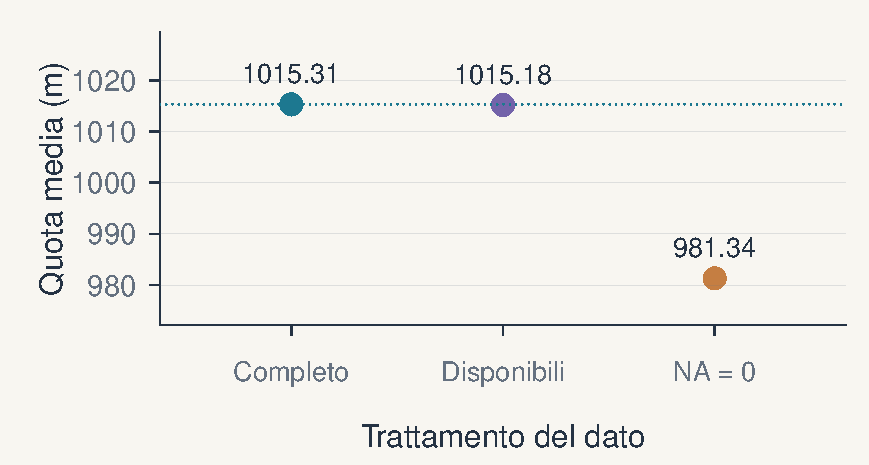
\includegraphics[width=9.85cm,height=5.25cm,keepaspectratio]{Risultati/Figure/05_effetto_zero.pdf}
\vspace{1.5mm}
\PSmall{Confronto fra terreno completo, celle disponibili e sostituzione impropria con zero. Le quantità hanno domini e significati diversi.}

\end{minipage}\end{lrbox}
\typeout{FULLBOX:024:PilotLeftBox:\the\ht\PilotLeftBox:\the\dp\PilotLeftBox}

\begin{lrbox}{\PilotRightBox}
\begin{minipage}[t]{7.55cm}\raggedright\color{Ink}\fontsize{11.3}{14.8}\selectfont
\PBody{La sostituzione aggiunge quote che non sono state osservate. Nel terreno del caso guida introduce valori molto inferiori alle quote circostanti.}
\vspace{2.5mm}
\PInfo{Il risultato numerico è calcolabile, ma la procedura cambia la variabile e la superficie rappresentata.}
\PCode{R · confronto dei significati}{024_esempio.R}
\end{minipage}\end{lrbox}
\typeout{FULLBOX:024:PilotRightBox:\the\ht\PilotRightBox:\the\dp\PilotRightBox}

\begin{tikzpicture}[remember picture,overlay]
\PilotChrome{Sostituire i mancanti con zero altera il risultato}{III · MASCHERE E DOMINIO}{24}{Una scelta di codifica non deve introdurre valori fisici inventati nelle statistiche.}
\node[anchor=north west,inner sep=0] at([xshift=.96cm,yshift=-2.13cm]current page.north west){\usebox{\PilotLeftBox}};
\node[anchor=north west,inner sep=0] at([xshift=11.52cm,yshift=-2.13cm]current page.north west){\usebox{\PilotRightBox}};
\node[anchor=north east,inner sep=0] at([xshift=17.65cm,yshift=-12.06cm]current page.north west){\color{Classical}\fontsize{7.7}{9.2}\selectfont\href{../../03_Notebook_svolti/M12_Tessera/M12_N04.html}{M12\_N04 · notebook svolto}};
\end{tikzpicture}\end{frame}

\begin{frame}[plain]\hypertarget{slide25}{}
\bookmark[level=1,page=25]{Ritagliare seleziona una parte del territorio}
\begin{lrbox}{\TitleBox}
\begin{minipage}[t]{17.7cm}\raggedright\color{Ink}\fontsize{11.3}{14.8}\selectfont
\color{Navy}\bfseries\fontsize{20.6}{24.5}\selectfont Ritagliare seleziona una parte del territorio
\end{minipage}\end{lrbox}
\typeout{FULLBOX:025:TitleBox:\the\ht\TitleBox:\the\dp\TitleBox}

\begin{lrbox}{\RecallBox}
\begin{minipage}[t]{14.3cm}\raggedright\color{Ink}\fontsize{11.3}{14.8}\selectfont
\fontsize{10.3}{13.8}\selectfont Il ritaglio è una scelta geografica da documentare insieme alla sintesi.
\end{minipage}\end{lrbox}
\typeout{FULLBOX:025:RecallBox:\the\ht\RecallBox:\the\dp\RecallBox}

\begin{lrbox}{\PilotLeftBox}
\begin{minipage}[t]{10.05cm}\raggedright\color{Ink}\fontsize{11.3}{14.8}\selectfont
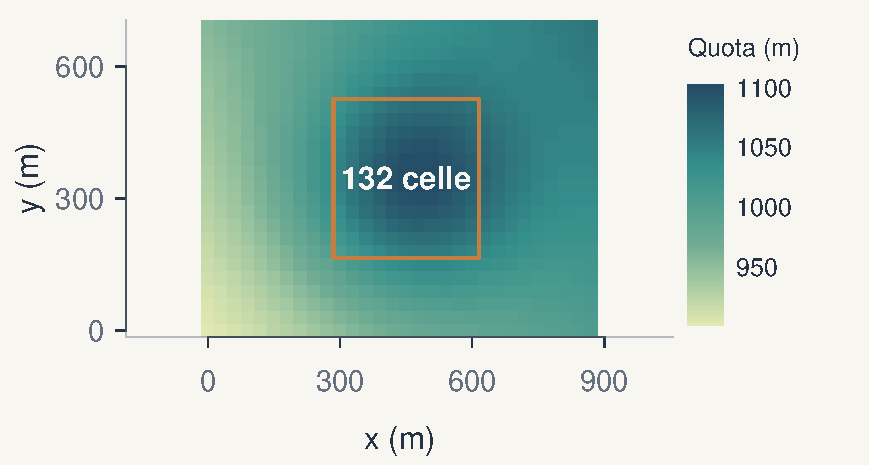
\includegraphics[width=9.85cm,height=5.25cm,keepaspectratio]{Risultati/Figure/06_ritaglio.pdf}
\vspace{1.5mm}
\PSmall{Selezione dei centri con 300 ≤ x ≤ 600 m e 180 ≤ y ≤ 510 m: 132 celle, pari a 11,88 ha nella griglia locale.}

\end{minipage}\end{lrbox}
\typeout{FULLBOX:025:PilotLeftBox:\the\ht\PilotLeftBox:\the\dp\PilotLeftBox}

\begin{lrbox}{\PilotRightBox}
\begin{minipage}[t]{7.55cm}\raggedright\color{Ink}\fontsize{11.3}{14.8}\selectfont
\PBody{La finestra contiene una parte diversa della morfologia. La sua media non risponde alla stessa domanda della media dell’intero dominio.}
\vspace{2.5mm}
\PInfo{Dichiariamo se il criterio riguarda i centri o l’intersezione con i bordi delle celle. Per confini irregolari le regole possono dare risultati diversi.}
\PCode{R · dominio dei centri}{025_esempio.R}
\end{minipage}\end{lrbox}
\typeout{FULLBOX:025:PilotRightBox:\the\ht\PilotRightBox:\the\dp\PilotRightBox}

\begin{tikzpicture}[remember picture,overlay]
\PilotChrome{Ritagliare seleziona una parte del territorio}{III · MASCHERE E DOMINIO}{25}{Il ritaglio è una scelta geografica da documentare insieme alla sintesi.}
\node[anchor=north west,inner sep=0] at([xshift=.96cm,yshift=-2.13cm]current page.north west){\usebox{\PilotLeftBox}};
\node[anchor=north west,inner sep=0] at([xshift=11.52cm,yshift=-2.13cm]current page.north west){\usebox{\PilotRightBox}};
\node[anchor=north east,inner sep=0] at([xshift=17.65cm,yshift=-12.06cm]current page.north west){\color{Classical}\fontsize{7.7}{9.2}\selectfont\href{../../03_Notebook_svolti/M12_Tessera/M12_N05.html}{M12\_N05 · notebook svolto}};
\end{tikzpicture}\end{frame}

\begin{frame}[plain]\hypertarget{slide26}{}
\bookmark[level=1,page=26]{Ritaglio e maschera hanno ruoli distinti}
\begin{lrbox}{\TitleBox}
\begin{minipage}[t]{17.7cm}\raggedright\color{Ink}\fontsize{11.3}{14.8}\selectfont
\color{Navy}\bfseries\fontsize{20.6}{24.5}\selectfont Ritaglio e maschera hanno ruoli distinti
\end{minipage}\end{lrbox}
\typeout{FULLBOX:026:TitleBox:\the\ht\TitleBox:\the\dp\TitleBox}

\begin{lrbox}{\RecallBox}
\begin{minipage}[t]{14.3cm}\raggedright\color{Ink}\fontsize{11.3}{14.8}\selectfont
\fontsize{10.3}{13.8}\selectfont Dimensione del file, estensione geometrica e superficie valida descrivono proprietà differenti.
\end{minipage}\end{lrbox}
\typeout{FULLBOX:026:RecallBox:\the\ht\RecallBox:\the\dp\RecallBox}

\begin{lrbox}{\PilotLeftBox}
\begin{minipage}[t]{10.05cm}\raggedright\color{Ink}\fontsize{11.3}{14.8}\selectfont
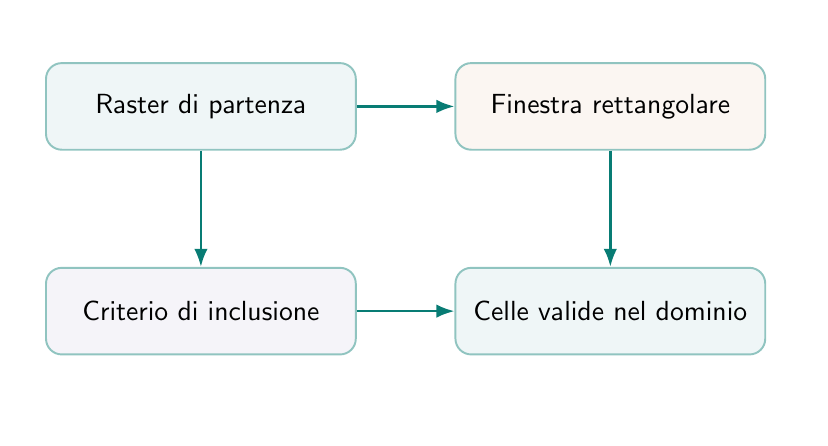
\begin{tikzpicture}[x=1cm,y=1cm]
\path[use as bounding box](-.1,-.15) rectangle(9.7,4.8);
\node[pFlow,text width=3.7cm,fill=GeoA!7] (a) at(2.1,3.8){Raster di partenza};
\node[pFlow,text width=3.7cm,fill=GeoB!7] (b) at(7.3,3.8){Finestra rettangolare};
\node[pFlow,text width=3.7cm,fill=GeoC!7] (c) at(2.1,1.2){Criterio di inclusione};
\node[pFlow,text width=3.7cm,fill=GeoA!7] (d) at(7.3,1.2){Celle valide nel dominio};
\draw[pEdge] (a) -- (b);
\draw[pEdge] (a) -- (c);
\draw[pEdge] (b) -- (d);
\draw[pEdge] (c) -- (d);
\end{tikzpicture}

\end{minipage}\end{lrbox}
\typeout{FULLBOX:026:PilotLeftBox:\the\ht\PilotLeftBox:\the\dp\PilotLeftBox}

\begin{lrbox}{\PilotRightBox}
\begin{minipage}[t]{7.55cm}\raggedright\color{Ink}\fontsize{11.3}{14.8}\selectfont
\PBody{Il ritaglio riduce l’estensione rettangolare. Una maschera può escludere celle al suo interno e descrivere un dominio irregolare.}
\vspace{2.5mm}
\PInfo{La superficie del rettangolo esterno e la superficie valida non sono necessariamente uguali. Le riportiamo separatamente.}
\PBody{Una geometria di ritaglio che attraversa celle richiede una regola di inclusione o un peso frazionario esplicito.}
\vspace{2.5mm}

\end{minipage}\end{lrbox}
\typeout{FULLBOX:026:PilotRightBox:\the\ht\PilotRightBox:\the\dp\PilotRightBox}

\begin{tikzpicture}[remember picture,overlay]
\PilotChrome{Ritaglio e maschera hanno ruoli distinti}{III · MASCHERE E DOMINIO}{26}{Dimensione del file, estensione geometrica e superficie valida descrivono proprietà differenti.}
\node[anchor=north west,inner sep=0] at([xshift=.96cm,yshift=-2.13cm]current page.north west){\usebox{\PilotLeftBox}};
\node[anchor=north west,inner sep=0] at([xshift=11.52cm,yshift=-2.13cm]current page.north west){\usebox{\PilotRightBox}};
\node[anchor=north east,inner sep=0] at([xshift=17.65cm,yshift=-12.06cm]current page.north west){\color{Classical}\fontsize{7.7}{9.2}\selectfont\href{../../03_Notebook_svolti/M12_Tessera/M12_N05.html}{M12\_N05 · notebook svolto}};
\end{tikzpicture}\end{frame}

\begin{frame}[plain]\hypertarget{slide27}{}
\bookmark[level=1,page=27]{Dal conteggio delle celle agli ettari}
\begin{lrbox}{\TitleBox}
\begin{minipage}[t]{17.7cm}\raggedright\color{Ink}\fontsize{11.3}{14.8}\selectfont
\color{Navy}\bfseries\fontsize{20.6}{24.5}\selectfont Dal conteggio delle celle agli ettari
\end{minipage}\end{lrbox}
\typeout{FULLBOX:027:TitleBox:\the\ht\TitleBox:\the\dp\TitleBox}

\begin{lrbox}{\RecallBox}
\begin{minipage}[t]{14.3cm}\raggedright\color{Ink}\fontsize{11.3}{14.8}\selectfont
\fontsize{10.3}{13.8}\selectfont La stessa parola «superficie» deve essere accompagnata dalla geometria a cui si riferisce.
\end{minipage}\end{lrbox}
\typeout{FULLBOX:027:RecallBox:\the\ht\RecallBox:\the\dp\RecallBox}

\begin{lrbox}{\PilotLeftBox}
\begin{minipage}[t]{10.05cm}\raggedright\color{Ink}\fontsize{11.3}{14.8}\selectfont
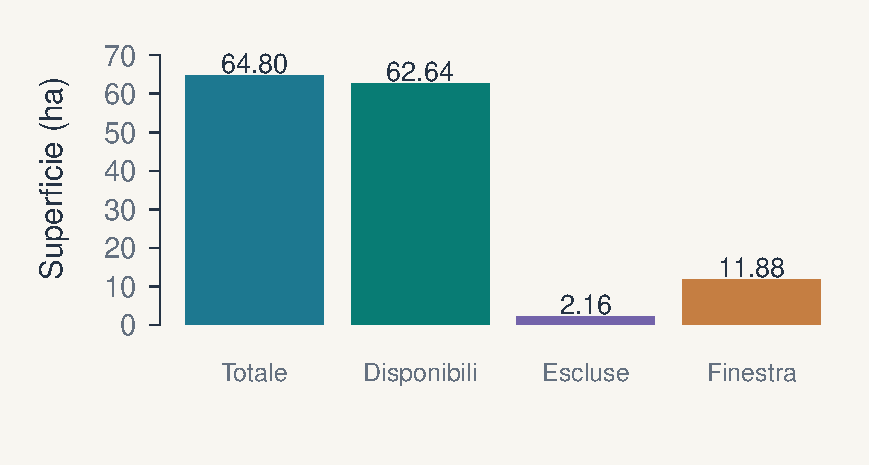
\includegraphics[width=9.85cm,height=4.65cm,keepaspectratio]{Risultati/Figure/07_superficie_zone.pdf}
\vspace{1.5mm}
\PSmall{Area piana dei domini: 720, 696, 24 e 132 celle rispettivamente.}
\[a=\Delta x\,\Delta y=900\ \mathrm{m}^2=0{,}09\ \mathrm{ha}\]

\end{minipage}\end{lrbox}
\typeout{FULLBOX:027:PilotLeftBox:\the\ht\PilotLeftBox:\the\dp\PilotLeftBox}

\begin{lrbox}{\PilotRightBox}
\begin{minipage}[t]{7.55cm}\raggedright\color{Ink}\fontsize{11.3}{14.8}\selectfont
\PBody{Il prodotto dei passi misura l’area piana della cella. La somma delle aree valide quantifica la copertura discretizzata.}
\vspace{2.5mm}
\PInfo{Questa area è planimetrica. Non è l’area reale della superficie inclinata del terreno.}
\PCode{R · area piana della griglia}{027_esempio.R}
\end{minipage}\end{lrbox}
\typeout{FULLBOX:027:PilotRightBox:\the\ht\PilotRightBox:\the\dp\PilotRightBox}

\begin{tikzpicture}[remember picture,overlay]
\PilotChrome{Dal conteggio delle celle agli ettari}{III · MASCHERE E DOMINIO}{27}{La stessa parola «superficie» deve essere accompagnata dalla geometria a cui si riferisce.}
\node[anchor=north west,inner sep=0] at([xshift=.96cm,yshift=-2.13cm]current page.north west){\usebox{\PilotLeftBox}};
\node[anchor=north west,inner sep=0] at([xshift=11.52cm,yshift=-2.13cm]current page.north west){\usebox{\PilotRightBox}};
\node[anchor=north east,inner sep=0] at([xshift=17.65cm,yshift=-12.06cm]current page.north west){\color{Classical}\fontsize{7.7}{9.2}\selectfont\href{../../03_Notebook_svolti/M12_Tessera/M12_N06.html}{M12\_N06 · notebook svolto}};
\end{tikzpicture}\end{frame}

\begin{frame}[plain]\hypertarget{slide28}{}
\bookmark[level=1,page=28]{Una griglia in gradi richiede un calcolo di area}
\begin{lrbox}{\TitleBox}
\begin{minipage}[t]{17.7cm}\raggedright\color{Ink}\fontsize{11.3}{14.8}\selectfont
\color{Navy}\bfseries\fontsize{20.6}{24.5}\selectfont Una griglia in gradi richiede un calcolo di area
\end{minipage}\end{lrbox}
\typeout{FULLBOX:028:TitleBox:\the\ht\TitleBox:\the\dp\TitleBox}

\begin{lrbox}{\RecallBox}
\begin{minipage}[t]{14.3cm}\raggedright\color{Ink}\fontsize{11.3}{14.8}\selectfont
\fontsize{10.3}{13.8}\selectfont La media semplice delle celle coincide con una media di area solo quando i pesi appropriati sono uguali.
\end{minipage}\end{lrbox}
\typeout{FULLBOX:028:RecallBox:\the\ht\RecallBox:\the\dp\RecallBox}

\begin{lrbox}{\PilotLeftBox}
\begin{minipage}[t]{10.05cm}\raggedright\color{Ink}\fontsize{11.3}{14.8}\selectfont
\[A_{\mathrm{valida}}=\sum_{k\in V}a_k\]
\[\overline z_A=\frac{\sum_{k\in V}a_k z_k}{\sum_{k\in V}a_k}\]
\PInfo{$a_k$ è l’area rappresentata dalla cella valida $k$. La media assume che i valori siano appropriati alla sintesi su quelle aree.}

\end{minipage}\end{lrbox}
\typeout{FULLBOX:028:PilotLeftBox:\the\ht\PilotLeftBox:\the\dp\PilotLeftBox}

\begin{lrbox}{\PilotRightBox}
\begin{minipage}[t]{7.55cm}\raggedright\color{Ink}\fontsize{11.3}{14.8}\selectfont
\PBody{Uguali intervalli angolari non definiscono celle di uguale area sulla Terra. Anche una proiezione può introdurre distorsioni di area.}
\vspace{2.5mm}
\PBody{Nel caso locale metrico usiamo l’area piana. Un’analisi geografica reale deve scegliere una misura di area coerente con il riferimento e con la domanda.}
\vspace{2.5mm}
\PSmall{La funzione terra::cellSize permette di calcolare aree tenendo conto della collocazione geografica; la scelta va documentata.}

\end{minipage}\end{lrbox}
\typeout{FULLBOX:028:PilotRightBox:\the\ht\PilotRightBox:\the\dp\PilotRightBox}

\begin{tikzpicture}[remember picture,overlay]
\PilotChrome{Una griglia in gradi richiede un calcolo di area}{III · MASCHERE E DOMINIO}{28}{La media semplice delle celle coincide con una media di area solo quando i pesi appropriati sono uguali.}
\node[anchor=north west,inner sep=0] at([xshift=.96cm,yshift=-2.13cm]current page.north west){\usebox{\PilotLeftBox}};
\node[anchor=north west,inner sep=0] at([xshift=11.52cm,yshift=-2.13cm]current page.north west){\usebox{\PilotRightBox}};
\node[anchor=north east,inner sep=0] at([xshift=17.65cm,yshift=-12.06cm]current page.north west){\color{Classical}\fontsize{7.7}{9.2}\selectfont\href{../../03_Notebook_svolti/M12_Tessera/M12_N06.html}{M12\_N06 · notebook svolto}};
\end{tikzpicture}\end{frame}

\begin{frame}[plain]\hypertarget{slide29}{}
\bookmark[level=1,page=29]{Le maschere si combinano conservando le cause}
\begin{lrbox}{\TitleBox}
\begin{minipage}[t]{17.7cm}\raggedright\color{Ink}\fontsize{11.3}{14.8}\selectfont
\color{Navy}\bfseries\fontsize{20.6}{24.5}\selectfont Le maschere si combinano conservando le cause
\end{minipage}\end{lrbox}
\typeout{FULLBOX:029:TitleBox:\the\ht\TitleBox:\the\dp\TitleBox}

\begin{lrbox}{\RecallBox}
\begin{minipage}[t]{14.3cm}\raggedright\color{Ink}\fontsize{11.3}{14.8}\selectfont
\fontsize{10.3}{13.8}\selectfont La tracciabilità della maschera spiega come cambia il dominio lungo la catena di elaborazione.
\end{minipage}\end{lrbox}
\typeout{FULLBOX:029:RecallBox:\the\ht\RecallBox:\the\dp\RecallBox}

\begin{lrbox}{\PilotLeftBox}
\begin{minipage}[t]{10.05cm}\raggedright\color{Ink}\fontsize{11.3}{14.8}\selectfont
{\fontsize{10.2}{13.1}\selectfont\renewcommand{\arraystretch}{1.45}\begin{tabular}{@{}p{4.1cm}p{4.9cm}@{}}\toprule
\textbf{Criterio} & \textbf{Informazione da registrare}\\\midrule
Valore disponibile & Assenza della misura\\
Qualità ammessa & Nuvole, saturazione o altro criterio\\
Dominio scelto & Inclusione territoriale\\
Calcolo definito & Vicinato o denominatore valido\\
Maschera finale & Intersezione dei criteri necessari\\
\bottomrule\end{tabular}}

\end{minipage}\end{lrbox}
\typeout{FULLBOX:029:PilotLeftBox:\the\ht\PilotLeftBox:\the\dp\PilotLeftBox}

\begin{lrbox}{\PilotRightBox}
\begin{minipage}[t]{7.55cm}\raggedright\color{Ink}\fontsize{11.3}{14.8}\selectfont
\PBody{La maschera complessiva può essere una congiunzione logica. Conservare i singoli motivi consente di capire perché una cella è stata esclusa.}
\vspace{2.5mm}
\PInfo{Quando calcoliamo una derivata, servono anche i vicini richiesti. Una cella con quota valida può avere una pendenza non calcolabile.}
\PBody{Le esclusioni introdotte dal metodo devono essere distinte dalle mancanze del dato originale.}
\vspace{2.5mm}

\end{minipage}\end{lrbox}
\typeout{FULLBOX:029:PilotRightBox:\the\ht\PilotRightBox:\the\dp\PilotRightBox}

\begin{tikzpicture}[remember picture,overlay]
\PilotChrome{Le maschere si combinano conservando le cause}{III · MASCHERE E DOMINIO}{29}{La tracciabilità della maschera spiega come cambia il dominio lungo la catena di elaborazione.}
\node[anchor=north west,inner sep=0] at([xshift=.96cm,yshift=-2.13cm]current page.north west){\usebox{\PilotLeftBox}};
\node[anchor=north west,inner sep=0] at([xshift=11.52cm,yshift=-2.13cm]current page.north west){\usebox{\PilotRightBox}};
\end{tikzpicture}\end{frame}

\begin{frame}[plain]\hypertarget{slide30}{}
\bookmark[level=1,page=30]{Una cella mancante può influenzare i vicini}
\begin{lrbox}{\TitleBox}
\begin{minipage}[t]{17.7cm}\raggedright\color{Ink}\fontsize{11.3}{14.8}\selectfont
\color{Navy}\bfseries\fontsize{20.6}{24.5}\selectfont Una cella mancante può influenzare i vicini
\end{minipage}\end{lrbox}
\typeout{FULLBOX:030:TitleBox:\the\ht\TitleBox:\the\dp\TitleBox}

\begin{lrbox}{\RecallBox}
\begin{minipage}[t]{14.3cm}\raggedright\color{Ink}\fontsize{11.3}{14.8}\selectfont
\fontsize{10.3}{13.8}\selectfont Il dominio di una grandezza derivata dipende dal vicinato necessario a calcolarla.
\end{minipage}\end{lrbox}
\typeout{FULLBOX:030:RecallBox:\the\ht\RecallBox:\the\dp\RecallBox}

\begin{lrbox}{\PilotLeftBox}
\begin{minipage}[t]{10.05cm}\raggedright\color{Ink}\fontsize{11.3}{14.8}\selectfont
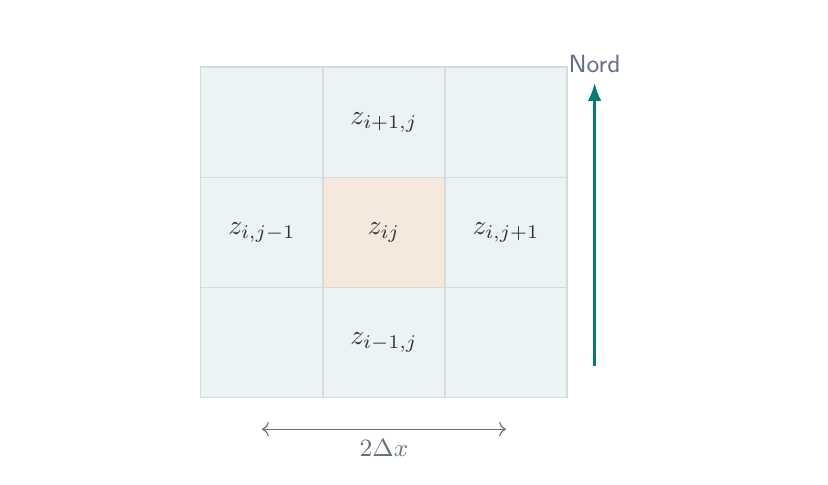
\begin{tikzpicture}[x=1cm,y=1cm]
\path[use as bounding box](-.1,-.15) rectangle(9.7,5.3);
\filldraw[fill=GeoA!9,draw=Rule](2.1,0.6)rectangle(3.6500000000000004,2.0);
\filldraw[fill=GeoA!9,draw=Rule](3.6500000000000004,0.6)rectangle(5.2,2.0);
\filldraw[fill=GeoA!9,draw=Rule](5.2,0.6)rectangle(6.75,2.0);
\filldraw[fill=GeoA!9,draw=Rule](2.1,2.0)rectangle(3.6500000000000004,3.4);
\filldraw[fill=GeoB!18,draw=Rule](3.6500000000000004,2.0)rectangle(5.2,3.4);
\filldraw[fill=GeoA!9,draw=Rule](5.2,2.0)rectangle(6.75,3.4);
\filldraw[fill=GeoA!9,draw=Rule](2.1,3.4)rectangle(3.6500000000000004,4.8);
\filldraw[fill=GeoA!9,draw=Rule](3.6500000000000004,3.4)rectangle(5.2,4.8);
\filldraw[fill=GeoA!9,draw=Rule](5.2,3.4)rectangle(6.75,4.8);
\node[pLabel]at(4.425,2.7){$z_{ij}$};
\node[pLabel]at(5.975,2.7){$z_{i,j+1}$};
\node[pLabel]at(2.875,2.7){$z_{i,j-1}$};
\node[pLabel]at(4.425,4.1){$z_{i+1,j}$};
\node[pLabel]at(4.425,1.3){$z_{i-1,j}$};
\draw[pEdge](7.1,1)--(7.1,4.6)node[above,pNote]{Nord};
\draw[<->,Muted](2.875,.2)--node[below,pNote]{$2\Delta x$}(5.975,.2);
\end{tikzpicture}

\end{minipage}\end{lrbox}
\typeout{FULLBOX:030:PilotLeftBox:\the\ht\PilotLeftBox:\the\dp\PilotLeftBox}

\begin{lrbox}{\PilotRightBox}
\begin{minipage}[t]{7.55cm}\raggedright\color{Ink}\fontsize{11.3}{14.8}\selectfont
\PBody{Il calcolo centrato utilizza quattro quote adiacenti. Se una di esse manca, la derivata richiesta non è disponibile.}
\vspace{2.5mm}
\PInfo{Adottiamo un criterio esplicito: centro valido e quattro vicini validi. Il bordo esterno richiede una convenzione separata.}
\PBody{Riempire automaticamente i buchi cambia il metodo e introduce un modello di interpolazione. La decisione deve essere motivata prima delle derivate.}
\vspace{2.5mm}

\end{minipage}\end{lrbox}
\typeout{FULLBOX:030:PilotRightBox:\the\ht\PilotRightBox:\the\dp\PilotRightBox}

\begin{tikzpicture}[remember picture,overlay]
\PilotChrome{Una cella mancante può influenzare i vicini}{III · MASCHERE E DOMINIO}{30}{Il dominio di una grandezza derivata dipende dal vicinato necessario a calcolarla.}
\node[anchor=north west,inner sep=0] at([xshift=.96cm,yshift=-2.13cm]current page.north west){\usebox{\PilotLeftBox}};
\node[anchor=north west,inner sep=0] at([xshift=11.52cm,yshift=-2.13cm]current page.north west){\usebox{\PilotRightBox}};
\end{tikzpicture}\end{frame}

\begin{frame}[plain]\hypertarget{slide31}{}
\bookmark[level=1,page=31]{Una sintesi riproducibile dichiara il denominatore}
\begin{lrbox}{\TitleBox}
\begin{minipage}[t]{17.7cm}\raggedright\color{Ink}\fontsize{11.3}{14.8}\selectfont
\color{Navy}\bfseries\fontsize{20.6}{24.5}\selectfont Una sintesi riproducibile dichiara il denominatore
\end{minipage}\end{lrbox}
\typeout{FULLBOX:031:TitleBox:\the\ht\TitleBox:\the\dp\TitleBox}

\begin{lrbox}{\RecallBox}
\begin{minipage}[t]{14.3cm}\raggedright\color{Ink}\fontsize{11.3}{14.8}\selectfont
\fontsize{10.3}{13.8}\selectfont Il denominatore fa parte della definizione scientifica della statistica.
\end{minipage}\end{lrbox}
\typeout{FULLBOX:031:RecallBox:\the\ht\RecallBox:\the\dp\RecallBox}

\begin{lrbox}{\PilotLeftBox}
\begin{minipage}[t]{10.05cm}\raggedright\color{Ink}\fontsize{11.3}{14.8}\selectfont
{\fontsize{10.2}{13.1}\selectfont\renewcommand{\arraystretch}{1.45}\begin{tabular}{@{}p{4.2cm}p{4.8cm}@{}}\toprule
\textbf{Quantità} & \textbf{Denominatore}\\\midrule
Copertura per numero & Celle ammesse nella griglia di riferimento\\
Media dei disponibili & Celle valide utilizzate\\
Media per area & Somma delle aree rappresentate\\
Frazione di una classe & Dominio valido definito\\
Densità territoriale & Area coerente con gli eventi contati\\
\bottomrule\end{tabular}}

\end{minipage}\end{lrbox}
\typeout{FULLBOX:031:PilotLeftBox:\the\ht\PilotLeftBox:\the\dp\PilotLeftBox}

\begin{lrbox}{\PilotRightBox}
\begin{minipage}[t]{7.55cm}\raggedright\color{Ink}\fontsize{11.3}{14.8}\selectfont
\PBody{Una percentuale o una media possono cambiare perché cambiano i valori, il dominio oppure entrambi.}
\vspace{2.5mm}
\PInfo{Nel confronto fra prodotti riportiamo i conteggi e usiamo, quando serve, una maschera comune. Confrontiamo così lo stesso insieme di celle.}
\PBody{Una mappa dei mancanti è spesso più informativa di una sola percentuale di copertura.}
\vspace{2.5mm}

\end{minipage}\end{lrbox}
\typeout{FULLBOX:031:PilotRightBox:\the\ht\PilotRightBox:\the\dp\PilotRightBox}

\begin{tikzpicture}[remember picture,overlay]
\PilotChrome{Una sintesi riproducibile dichiara il denominatore}{III · MASCHERE E DOMINIO}{31}{Il denominatore fa parte della definizione scientifica della statistica.}
\node[anchor=north west,inner sep=0] at([xshift=.96cm,yshift=-2.13cm]current page.north west){\usebox{\PilotLeftBox}};
\node[anchor=north west,inner sep=0] at([xshift=11.52cm,yshift=-2.13cm]current page.north west){\usebox{\PilotRightBox}};
\node[anchor=north east,inner sep=0] at([xshift=17.65cm,yshift=-12.06cm]current page.north west){\color{Classical}\fontsize{7.7}{9.2}\selectfont\href{../../03_Notebook_svolti/M12_Tessera/M12_N06.html}{M12\_N06 · notebook svolto}};
\end{tikzpicture}\end{frame}

\begin{frame}[plain]\hypertarget{slide32}{}
\bookmark[level=1,page=32]{Laboratorio: conservare il dominio osservato}
\begin{lrbox}{\TitleBox}
\begin{minipage}[t]{17.7cm}\raggedright\color{Ink}\fontsize{11.3}{14.8}\selectfont
\color{Navy}\bfseries\fontsize{20.6}{24.5}\selectfont Laboratorio: conservare il dominio osservato
\end{minipage}\end{lrbox}
\typeout{FULLBOX:032:TitleBox:\the\ht\TitleBox:\the\dp\TitleBox}

\begin{lrbox}{\RecallBox}
\begin{minipage}[t]{14.3cm}\raggedright\color{Ink}\fontsize{11.3}{14.8}\selectfont
\fontsize{10.3}{13.8}\selectfont Le celle escluse devono rimanere riconoscibili dopo ogni passaggio.
\end{minipage}\end{lrbox}
\typeout{FULLBOX:032:RecallBox:\the\ht\RecallBox:\the\dp\RecallBox}

\begin{lrbox}{\PilotLeftBox}
\begin{minipage}[t]{10.05cm}\raggedright\color{Ink}\fontsize{11.3}{14.8}\selectfont
\PLab{https://marzione00.github.io/Lab_Geo/\#laboratorio/m12-maschere}{Esperimento online · maschere e superficie}
{\fontsize{10.2}{13.1}\selectfont\renewcommand{\arraystretch}{1.45}\begin{tabular}{@{}p{4.2cm}p{4.8cm}@{}}\toprule
\textbf{Attività} & \textbf{Controllo}\\\midrule
N04: NoData & 24 celle mancanti, zero distinto\\
N05: ritaglio & 132 centri inclusi nella finestra\\
N06: area & 900 m² per cella nel piano\\
Consegna & Quote, maschera e copertura\\
Interpretazione & Dominio al quale si riferisce la media\\
\bottomrule\end{tabular}}

\end{minipage}\end{lrbox}
\typeout{FULLBOX:032:PilotLeftBox:\the\ht\PilotLeftBox:\the\dp\PilotLeftBox}

\begin{lrbox}{\PilotRightBox}
\begin{minipage}[t]{7.55cm}\raggedright\color{Ink}\fontsize{11.3}{14.8}\selectfont
\PBody{La consegna permette di ricostruire le esclusioni e il loro effetto. Ogni confronto conserva la definizione del dominio.}
\vspace{2.5mm}
\PInfo{Passare a una nuova risoluzione cambierà il modo in cui le celle rappresentano quel dominio. La maschera dovrà seguire anche questa trasformazione.}

\end{minipage}\end{lrbox}
\typeout{FULLBOX:032:PilotRightBox:\the\ht\PilotRightBox:\the\dp\PilotRightBox}

\begin{tikzpicture}[remember picture,overlay]
\PilotChrome{Laboratorio: conservare il dominio osservato}{III · MASCHERE E DOMINIO}{32}{Le celle escluse devono rimanere riconoscibili dopo ogni passaggio.}
\node[anchor=north west,inner sep=0] at([xshift=.96cm,yshift=-2.13cm]current page.north west){\usebox{\PilotLeftBox}};
\node[anchor=north west,inner sep=0] at([xshift=11.52cm,yshift=-2.13cm]current page.north west){\usebox{\PilotRightBox}};
\node[anchor=north east,inner sep=0] at([xshift=17.65cm,yshift=-12.06cm]current page.north west){\color{Classical}\fontsize{7.7}{9.2}\selectfont\href{../../03_Notebook_svolti/M12_Tessera/M12_N06.html}{M12\_N06 · notebook svolto}};
\end{tikzpicture}\end{frame}

\begin{frame}[plain]\hypertarget{slide33}{}
\bookmark[level=0,page=33]{IV · RISOLUZIONE E ALLINEAMENTO}
\bookmark[level=1,page=33]{Cambiare griglia richiede di scegliere l’operazione}
\begin{lrbox}{\TitleBox}
\begin{minipage}[t]{17.7cm}\raggedright\color{Ink}\fontsize{11.3}{14.8}\selectfont
\color{Navy}\bfseries\fontsize{20.6}{24.5}\selectfont Cambiare griglia richiede di scegliere l’operazione
\end{minipage}\end{lrbox}
\typeout{FULLBOX:033:TitleBox:\the\ht\TitleBox:\the\dp\TitleBox}

\begin{lrbox}{\RecallBox}
\begin{minipage}[t]{14.3cm}\raggedright\color{Ink}\fontsize{11.3}{14.8}\selectfont
\fontsize{10.3}{13.8}\selectfont La trasformazione della griglia e quella dei valori devono essere documentate insieme.
\end{minipage}\end{lrbox}
\typeout{FULLBOX:033:RecallBox:\the\ht\RecallBox:\the\dp\RecallBox}

\begin{lrbox}{\PilotLeftBox}
\begin{minipage}[t]{10.05cm}\raggedright\color{Ink}\fontsize{11.3}{14.8}\selectfont
{\fontsize{10.2}{13.1}\selectfont\renewcommand{\arraystretch}{1.45}\begin{tabular}{@{}p{3.6cm}p{5.4cm}@{}}\toprule
\textbf{Operazione} & \textbf{Scopo}\\\midrule
Aggregare & Riassumere gruppi di celle\\
Disaggregare & Suddividere la geometria delle celle\\
Ricampionare & Stimare valori su una griglia diversa\\
Riproiettare & Trasformare il riferimento e definire l’uscita\\
Ritagliare & Selezionare un’estensione\\
\bottomrule\end{tabular}}

\end{minipage}\end{lrbox}
\typeout{FULLBOX:033:PilotLeftBox:\the\ht\PilotLeftBox:\the\dp\PilotLeftBox}

\begin{lrbox}{\PilotRightBox}
\begin{minipage}[t]{7.55cm}\raggedright\color{Ink}\fontsize{11.3}{14.8}\selectfont
\PBody{Le operazioni possono produrre immagini simili ma hanno significati differenti. Esplicitiamo sempre griglia di partenza, griglia di arrivo e regola per i valori.}
\vspace{2.5mm}
\PInfo{La geometria obiettivo include passo, origine, estensione e CRS. Un numero di righe e colonne non è sufficiente.}
\PBody{Il metodo dipende anche dal tipo di variabile: quota continua, categoria o quantità da conservare.}
\vspace{2.5mm}

\end{minipage}\end{lrbox}
\typeout{FULLBOX:033:PilotRightBox:\the\ht\PilotRightBox:\the\dp\PilotRightBox}

\begin{tikzpicture}[remember picture,overlay]
\PilotChrome{Cambiare griglia richiede di scegliere l’operazione}{IV · RISOLUZIONE E ALLINEAMENTO}{33}{La trasformazione della griglia e quella dei valori devono essere documentate insieme.}
\node[anchor=north west,inner sep=0] at([xshift=.96cm,yshift=-2.13cm]current page.north west){\usebox{\PilotLeftBox}};
\node[anchor=north west,inner sep=0] at([xshift=11.52cm,yshift=-2.13cm]current page.north west){\usebox{\PilotRightBox}};
\end{tikzpicture}\end{frame}

\begin{frame}[plain]\hypertarget{slide34}{}
\bookmark[level=1,page=34]{Quattro celle diventano una media}
\begin{lrbox}{\TitleBox}
\begin{minipage}[t]{17.7cm}\raggedright\color{Ink}\fontsize{11.3}{14.8}\selectfont
\color{Navy}\bfseries\fontsize{20.6}{24.5}\selectfont Quattro celle diventano una media
\end{minipage}\end{lrbox}
\typeout{FULLBOX:034:TitleBox:\the\ht\TitleBox:\the\dp\TitleBox}

\begin{lrbox}{\RecallBox}
\begin{minipage}[t]{14.3cm}\raggedright\color{Ink}\fontsize{11.3}{14.8}\selectfont
\fontsize{10.3}{13.8}\selectfont Una cella aggregata ha un supporto diverso da quello dei valori di partenza.
\end{minipage}\end{lrbox}
\typeout{FULLBOX:034:RecallBox:\the\ht\RecallBox:\the\dp\RecallBox}

\begin{lrbox}{\FullWideBox}
\begin{minipage}[t]{18.1cm}\raggedright\color{Ink}\fontsize{11.3}{14.8}\selectfont
\centering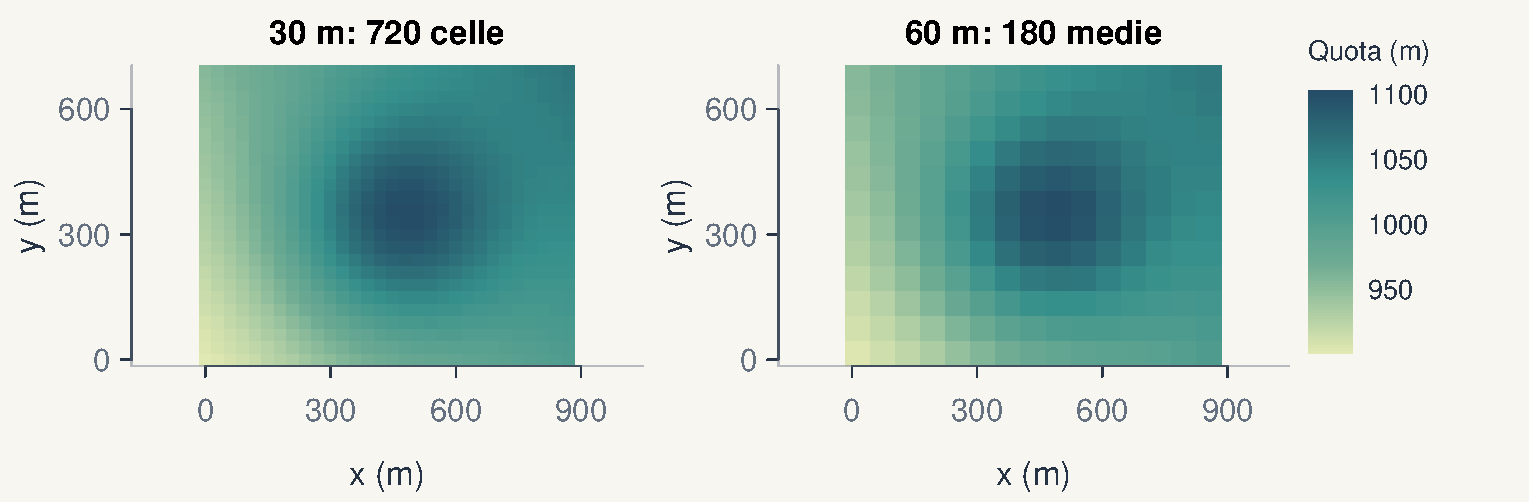
\includegraphics[width=18.05cm,height=5.8cm,keepaspectratio]{Risultati/Figure/08_aggregazione.pdf}
\end{minipage}\end{lrbox}
\typeout{FULLBOX:034:FullWideBox:\the\ht\FullWideBox:\the\dp\FullWideBox}

\begin{lrbox}{\PilotRightBox}
\begin{minipage}[t]{18.1cm}\raggedright\color{Ink}\fontsize{11.3}{14.8}\selectfont
\PBody{Griglia da 30 m: 24×30 celle. Aggregazione 2×2: 12×15 medie su celle da 60 m. Estensione e scala cromatica restano comuni. La media globale si conserva perché ogni blocco completo comprende quattro valori con uguale peso; estremi e dettaglio morfologico possono cambiare.}
\end{minipage}\end{lrbox}
\typeout{FULLBOX:034:PilotRightBox:\the\ht\PilotRightBox:\the\dp\PilotRightBox}

\begin{tikzpicture}[remember picture,overlay]
\PilotChrome{Quattro celle diventano una media}{IV · RISOLUZIONE E ALLINEAMENTO}{34}{Una cella aggregata ha un supporto diverso da quello dei valori di partenza.}
\node[anchor=north west,inner sep=0] at([xshift=.96cm,yshift=-2.13cm]current page.north west){\usebox{\FullWideBox}};
\node[anchor=north west,inner sep=0] at([xshift=.96cm,yshift=-8.25cm]current page.north west){\usebox{\PilotRightBox}};
\node[anchor=north east,inner sep=0] at([xshift=17.65cm,yshift=-12.06cm]current page.north west){\color{Classical}\fontsize{7.7}{9.2}\selectfont\href{../../03_Notebook_svolti/M12_Tessera/M12_N07.html}{M12\_N07 · notebook svolto}};
\end{tikzpicture}\end{frame}

\begin{frame}[plain]\hypertarget{slide35}{}
\bookmark[level=1,page=35]{La conservazione della media deriva dai pesi}
\begin{lrbox}{\TitleBox}
\begin{minipage}[t]{17.7cm}\raggedright\color{Ink}\fontsize{11.3}{14.8}\selectfont
\color{Navy}\bfseries\fontsize{20.6}{24.5}\selectfont La conservazione della media deriva dai pesi
\end{minipage}\end{lrbox}
\typeout{FULLBOX:035:TitleBox:\the\ht\TitleBox:\the\dp\TitleBox}

\begin{lrbox}{\RecallBox}
\begin{minipage}[t]{14.3cm}\raggedright\color{Ink}\fontsize{11.3}{14.8}\selectfont
\fontsize{10.3}{13.8}\selectfont La media globale si conserva perché ogni valore di partenza riceve lo stesso peso finale.
\end{minipage}\end{lrbox}
\typeout{FULLBOX:035:RecallBox:\the\ht\RecallBox:\the\dp\RecallBox}

\begin{lrbox}{\PilotLeftBox}
\begin{minipage}[t]{10.05cm}\raggedright\color{Ink}\fontsize{11.3}{14.8}\selectfont
\[\overline z_b=\frac14\sum_{k\in b}z_k\]
\[\frac1{180}\sum_{b=1}^{180}\overline z_b
       =\frac1{720}\sum_{k=1}^{720}z_k\]
\PInfo{La relazione vale per 180 blocchi completi, ciascuno formato da quattro celle con lo stesso peso.}

\end{minipage}\end{lrbox}
\typeout{FULLBOX:035:PilotLeftBox:\the\ht\PilotLeftBox:\the\dp\PilotLeftBox}

\begin{lrbox}{\PilotRightBox}
\begin{minipage}[t]{7.55cm}\raggedright\color{Ink}\fontsize{11.3}{14.8}\selectfont
\PBody{Il risultato è un’identità algebrica. Non dimostra che le distribuzioni o le forme locali del terreno restino uguali.}
\vspace{2.5mm}
\PSmall{Verifichiamo separatamente media, intervallo dei valori, risoluzione ed estensione.}
\PCode{R · aggregare e verificare}{035_esempio.R}
\end{minipage}\end{lrbox}
\typeout{FULLBOX:035:PilotRightBox:\the\ht\PilotRightBox:\the\dp\PilotRightBox}

\begin{tikzpicture}[remember picture,overlay]
\PilotChrome{La conservazione della media deriva dai pesi}{IV · RISOLUZIONE E ALLINEAMENTO}{35}{La media globale si conserva perché ogni valore di partenza riceve lo stesso peso finale.}
\node[anchor=north west,inner sep=0] at([xshift=.96cm,yshift=-2.13cm]current page.north west){\usebox{\PilotLeftBox}};
\node[anchor=north west,inner sep=0] at([xshift=11.52cm,yshift=-2.13cm]current page.north west){\usebox{\PilotRightBox}};
\node[anchor=north east,inner sep=0] at([xshift=17.65cm,yshift=-12.06cm]current page.north west){\color{Classical}\fontsize{7.7}{9.2}\selectfont\href{../../03_Notebook_svolti/M12_Tessera/M12_N07.html}{M12\_N07 · notebook svolto}};
\end{tikzpicture}\end{frame}

\begin{frame}[plain]\hypertarget{slide36}{}
\bookmark[level=1,page=36]{I blocchi con mancanti possono avere pesi diversi}
\begin{lrbox}{\TitleBox}
\begin{minipage}[t]{17.7cm}\raggedright\color{Ink}\fontsize{11.3}{14.8}\selectfont
\color{Navy}\bfseries\fontsize{20.6}{24.5}\selectfont I blocchi con mancanti possono avere pesi diversi
\end{minipage}\end{lrbox}
\typeout{FULLBOX:036:TitleBox:\the\ht\TitleBox:\the\dp\TitleBox}

\begin{lrbox}{\RecallBox}
\begin{minipage}[t]{14.3cm}\raggedright\color{Ink}\fontsize{11.3}{14.8}\selectfont
\fontsize{10.3}{13.8}\selectfont Il conteggio delle celle valide deve accompagnare il valore di ogni blocco.
\end{minipage}\end{lrbox}
\typeout{FULLBOX:036:RecallBox:\the\ht\RecallBox:\the\dp\RecallBox}

\begin{lrbox}{\PilotLeftBox}
\begin{minipage}[t]{10.05cm}\raggedright\color{Ink}\fontsize{11.3}{14.8}\selectfont
\[\overline z_{\mathrm{disp}}
 =\frac{\sum_b n_b\,\overline z_b}{\sum_b n_b}\]
{\fontsize{10.2}{13.1}\selectfont\renewcommand{\arraystretch}{1.45}\begin{tabular}{@{}p{3.8cm}p{2.2cm}p{2.7cm}@{}}\toprule
\textbf{Blocco} & \textbf{Valori validi} & \textbf{Media}\\\midrule
A & 1 & 10\\
B & 3 & 20\\
Media dei quattro valori & 4 & 17,5\\
Media semplice dei blocchi & 2 blocchi & 15\\
\bottomrule\end{tabular}}

\end{minipage}\end{lrbox}
\typeout{FULLBOX:036:PilotLeftBox:\the\ht\PilotLeftBox:\the\dp\PilotLeftBox}

\begin{lrbox}{\PilotRightBox}
\begin{minipage}[t]{7.55cm}\raggedright\color{Ink}\fontsize{11.3}{14.8}\selectfont
\PBody{Dopo na.rm=TRUE, due medie di blocco possono riassumere quantità diverse di celle valide. La loro media semplice cambia i pesi.}
\vspace{2.5mm}
\PInfo{Pesare per $n_b$ ricostruisce la media dei disponibili. Per inferire la media del dominio completo occorrono ulteriori ipotesi sulla mancanza.}
\PCode{R · due pesature}{036_esempio.R}
\end{minipage}\end{lrbox}
\typeout{FULLBOX:036:PilotRightBox:\the\ht\PilotRightBox:\the\dp\PilotRightBox}

\begin{tikzpicture}[remember picture,overlay]
\PilotChrome{I blocchi con mancanti possono avere pesi diversi}{IV · RISOLUZIONE E ALLINEAMENTO}{36}{Il conteggio delle celle valide deve accompagnare il valore di ogni blocco.}
\node[anchor=north west,inner sep=0] at([xshift=.96cm,yshift=-2.13cm]current page.north west){\usebox{\PilotLeftBox}};
\node[anchor=north west,inner sep=0] at([xshift=11.52cm,yshift=-2.13cm]current page.north west){\usebox{\PilotRightBox}};
\node[anchor=north east,inner sep=0] at([xshift=17.65cm,yshift=-12.06cm]current page.north west){\color{Classical}\fontsize{7.7}{9.2}\selectfont\href{../../03_Notebook_svolti/M12_Tessera/M12_N07.html}{M12\_N07 · notebook svolto}};
\end{tikzpicture}\end{frame}

\begin{frame}[plain]\hypertarget{slide37}{}
\bookmark[level=1,page=37]{Un massimo aggregato descrive una scala diversa}
\begin{lrbox}{\TitleBox}
\begin{minipage}[t]{17.7cm}\raggedright\color{Ink}\fontsize{11.3}{14.8}\selectfont
\color{Navy}\bfseries\fontsize{20.6}{24.5}\selectfont Un massimo aggregato descrive una scala diversa
\end{minipage}\end{lrbox}
\typeout{FULLBOX:037:TitleBox:\the\ht\TitleBox:\the\dp\TitleBox}

\begin{lrbox}{\RecallBox}
\begin{minipage}[t]{14.3cm}\raggedright\color{Ink}\fontsize{11.3}{14.8}\selectfont
\fontsize{10.3}{13.8}\selectfont La perdita di dettaglio morfologico può essere rilevante anche quando la media globale rimane identica.
\end{minipage}\end{lrbox}
\typeout{FULLBOX:037:RecallBox:\the\ht\RecallBox:\the\dp\RecallBox}

\begin{lrbox}{\PilotLeftBox}
\begin{minipage}[t]{10.05cm}\raggedright\color{Ink}\fontsize{11.3}{14.8}\selectfont
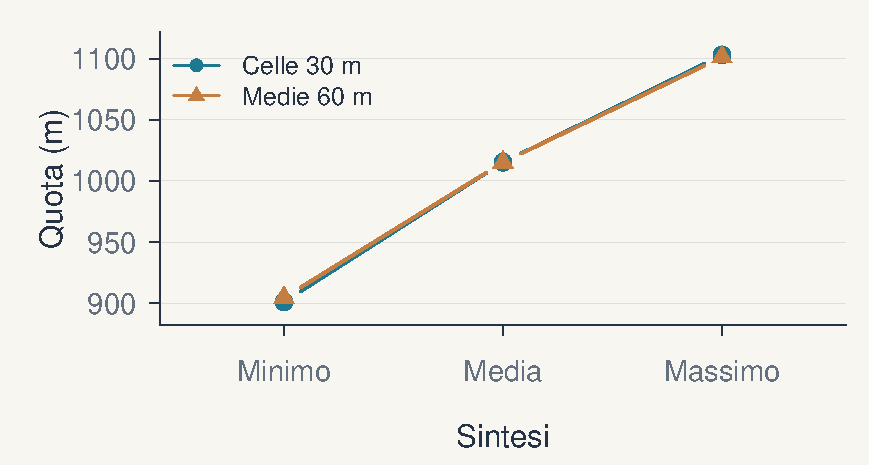
\includegraphics[width=9.85cm,height=5.25cm,keepaspectratio]{Risultati/Figure/09_perdita_estremi.pdf}
\vspace{1.5mm}
\PSmall{Minimo, media e massimo prima e dopo l’aggregazione. Le differenze sono calcolate sullo stesso dominio.}

\end{minipage}\end{lrbox}
\typeout{FULLBOX:037:PilotLeftBox:\the\ht\PilotLeftBox:\the\dp\PilotLeftBox}

\begin{lrbox}{\PilotRightBox}
\begin{minipage}[t]{7.55cm}\raggedright\color{Ink}\fontsize{11.3}{14.8}\selectfont
\PBody{La media di un blocco è compresa fra i suoi valori estremi. Di conseguenza il massimo delle medie non può superare il massimo originale.}
\vspace{2.5mm}
\PInfo{Una cima stretta può attenuarsi nella griglia aggregata. La sua minore quota rappresentata non implica un cambiamento del terreno.}
\PBody{Le differenze dipendono da come le forme si collocano rispetto ai blocchi e dalla scala scelta.}
\vspace{2.5mm}

\end{minipage}\end{lrbox}
\typeout{FULLBOX:037:PilotRightBox:\the\ht\PilotRightBox:\the\dp\PilotRightBox}

\begin{tikzpicture}[remember picture,overlay]
\PilotChrome{Un massimo aggregato descrive una scala diversa}{IV · RISOLUZIONE E ALLINEAMENTO}{37}{La perdita di dettaglio morfologico può essere rilevante anche quando la media globale rimane identica.}
\node[anchor=north west,inner sep=0] at([xshift=.96cm,yshift=-2.13cm]current page.north west){\usebox{\PilotLeftBox}};
\node[anchor=north west,inner sep=0] at([xshift=11.52cm,yshift=-2.13cm]current page.north west){\usebox{\PilotRightBox}};
\node[anchor=north east,inner sep=0] at([xshift=17.65cm,yshift=-12.06cm]current page.north west){\color{Classical}\fontsize{7.7}{9.2}\selectfont\href{../../03_Notebook_svolti/M12_Tessera/M12_N07.html}{M12\_N07 · notebook svolto}};
\end{tikzpicture}\end{frame}

\begin{frame}[plain]\hypertarget{slide38}{}
\bookmark[level=1,page=38]{Più celle memorizzate non aggiungono misure}
\begin{lrbox}{\TitleBox}
\begin{minipage}[t]{17.7cm}\raggedright\color{Ink}\fontsize{11.3}{14.8}\selectfont
\color{Navy}\bfseries\fontsize{20.6}{24.5}\selectfont Più celle memorizzate non aggiungono misure
\end{minipage}\end{lrbox}
\typeout{FULLBOX:038:TitleBox:\the\ht\TitleBox:\the\dp\TitleBox}

\begin{lrbox}{\RecallBox}
\begin{minipage}[t]{14.3cm}\raggedright\color{Ink}\fontsize{11.3}{14.8}\selectfont
\fontsize{10.3}{13.8}\selectfont Una griglia più fitta descrive una scelta di rappresentazione e di calcolo.
\end{minipage}\end{lrbox}
\typeout{FULLBOX:038:RecallBox:\the\ht\RecallBox:\the\dp\RecallBox}

\begin{lrbox}{\PilotLeftBox}
\begin{minipage}[t]{10.05cm}\raggedright\color{Ink}\fontsize{11.3}{14.8}\selectfont
\[n_{\mathrm{nuovo}}=n_{\mathrm{origine}}
 \left(\frac{\Delta_{\mathrm{origine}}}{\Delta_{\mathrm{nuovo}}}\right)^2\]
\PInfo{Relazione per celle quadrate sullo stesso dominio, con suddivisione compatibile. Da 30 a 10 m, il conteggio cresce di un fattore nove.}

\end{minipage}\end{lrbox}
\typeout{FULLBOX:038:PilotLeftBox:\the\ht\PilotLeftBox:\the\dp\PilotLeftBox}

\begin{lrbox}{\PilotRightBox}
\begin{minipage}[t]{7.55cm}\raggedright\color{Ink}\fontsize{11.3}{14.8}\selectfont
\PBody{La disaggregazione può copiare i valori oppure un ricampionamento può interpolarli. In entrambi i casi il dato originario resta quello della griglia di partenza.}
\vspace{2.5mm}
\PBody{Una rappresentazione più fitta può essere utile per allineare prodotti, ma non giustifica interpretazioni a una nuova scala di misura.}
\vspace{2.5mm}
\PSmall{Dimensione del pixel in uscita e capacità di risolvere strutture vicine devono restare distinte.}

\end{minipage}\end{lrbox}
\typeout{FULLBOX:038:PilotRightBox:\the\ht\PilotRightBox:\the\dp\PilotRightBox}

\begin{tikzpicture}[remember picture,overlay]
\PilotChrome{Più celle memorizzate non aggiungono misure}{IV · RISOLUZIONE E ALLINEAMENTO}{38}{Una griglia più fitta descrive una scelta di rappresentazione e di calcolo.}
\node[anchor=north west,inner sep=0] at([xshift=.96cm,yshift=-2.13cm]current page.north west){\usebox{\PilotLeftBox}};
\node[anchor=north west,inner sep=0] at([xshift=11.52cm,yshift=-2.13cm]current page.north west){\usebox{\PilotRightBox}};
\end{tikzpicture}\end{frame}

\begin{frame}[plain]\hypertarget{slide39}{}
\bookmark[level=1,page=39]{Interpolare una superficie continua}
\begin{lrbox}{\TitleBox}
\begin{minipage}[t]{17.7cm}\raggedright\color{Ink}\fontsize{11.3}{14.8}\selectfont
\color{Navy}\bfseries\fontsize{20.6}{24.5}\selectfont Interpolare una superficie continua
\end{minipage}\end{lrbox}
\typeout{FULLBOX:039:TitleBox:\the\ht\TitleBox:\the\dp\TitleBox}

\begin{lrbox}{\RecallBox}
\begin{minipage}[t]{14.3cm}\raggedright\color{Ink}\fontsize{11.3}{14.8}\selectfont
\fontsize{10.3}{13.8}\selectfont Il metodo di ricampionamento deve essere coerente con la variabile e con il compito.
\end{minipage}\end{lrbox}
\typeout{FULLBOX:039:RecallBox:\the\ht\RecallBox:\the\dp\RecallBox}

\begin{lrbox}{\FullWideBox}
\begin{minipage}[t]{18.1cm}\raggedright\color{Ink}\fontsize{11.3}{14.8}\selectfont
\centering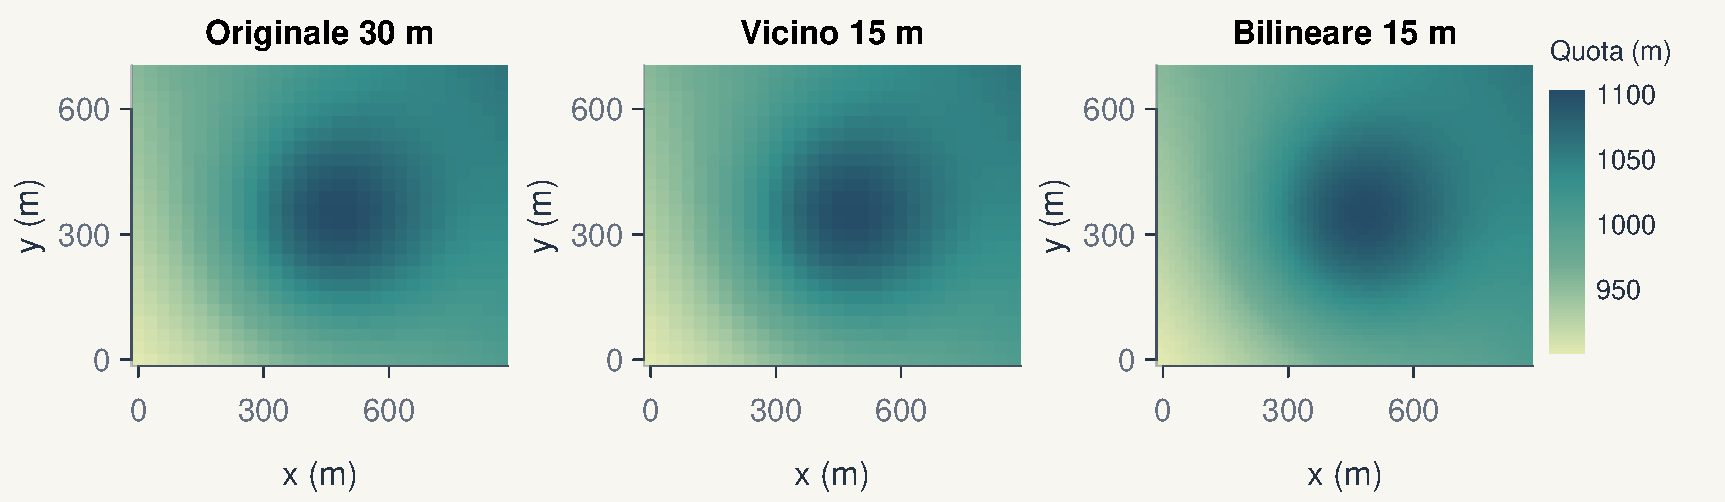
\includegraphics[width=18.05cm,height=5.8cm,keepaspectratio]{Risultati/Figure/12_ricampionamento_continuo.pdf}
\end{minipage}\end{lrbox}
\typeout{FULLBOX:039:FullWideBox:\the\ht\FullWideBox:\the\dp\FullWideBox}

\begin{lrbox}{\PilotRightBox}
\begin{minipage}[t]{18.1cm}\raggedright\color{Ink}\fontsize{11.3}{14.8}\selectfont
\PBody{Griglia originale da 30 m e griglie di uscita da 15 m, ottenute con vicino più prossimo e interpolazione bilineare realmente eseguiti in terra. Il numero di celle e la levigatezza cambiano; le misure disponibili restano quelle del raster originale. Bordi e mancanti richiedono regole esplicite.}
\end{minipage}\end{lrbox}
\typeout{FULLBOX:039:PilotRightBox:\the\ht\PilotRightBox:\the\dp\PilotRightBox}

\begin{tikzpicture}[remember picture,overlay]
\PilotChrome{Interpolare una superficie continua}{IV · RISOLUZIONE E ALLINEAMENTO}{39}{Il metodo di ricampionamento deve essere coerente con la variabile e con il compito.}
\node[anchor=north west,inner sep=0] at([xshift=.96cm,yshift=-2.13cm]current page.north west){\usebox{\FullWideBox}};
\node[anchor=north west,inner sep=0] at([xshift=.96cm,yshift=-8.25cm]current page.north west){\usebox{\PilotRightBox}};
\node[anchor=north east,inner sep=0] at([xshift=17.65cm,yshift=-12.06cm]current page.north west){\color{Classical}\fontsize{7.7}{9.2}\selectfont\href{../../03_Notebook_svolti/M12_Tessera/M12_N08.html}{M12\_N08 · notebook svolto}};
\end{tikzpicture}\end{frame}

\begin{frame}[plain]\hypertarget{slide40}{}
\bookmark[level=1,page=40]{La combinazione bilineare usa pesi geometrici}
\begin{lrbox}{\TitleBox}
\begin{minipage}[t]{17.7cm}\raggedright\color{Ink}\fontsize{11.3}{14.8}\selectfont
\color{Navy}\bfseries\fontsize{20.6}{24.5}\selectfont La combinazione bilineare usa pesi geometrici
\end{minipage}\end{lrbox}
\typeout{FULLBOX:040:TitleBox:\the\ht\TitleBox:\the\dp\TitleBox}

\begin{lrbox}{\RecallBox}
\begin{minipage}[t]{14.3cm}\raggedright\color{Ink}\fontsize{11.3}{14.8}\selectfont
\fontsize{10.3}{13.8}\selectfont I pesi rendono verificabili le proprietà della regola di interpolazione.
\end{minipage}\end{lrbox}
\typeout{FULLBOX:040:RecallBox:\the\ht\RecallBox:\the\dp\RecallBox}

\begin{lrbox}{\PilotLeftBox}
\begin{minipage}[t]{10.05cm}\raggedright\color{Ink}\fontsize{11.3}{14.8}\selectfont
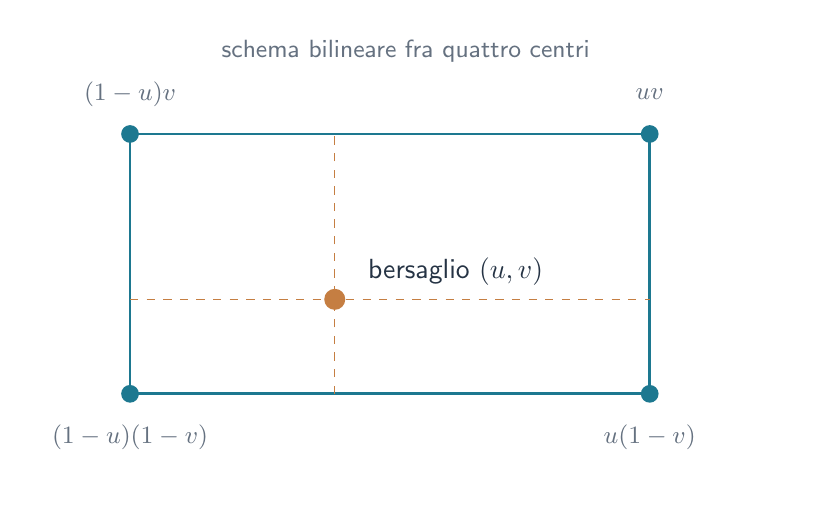
\begin{tikzpicture}[x=1cm,y=1cm]
\path[use as bounding box](-.1,-.15) rectangle(9.7,5.65);
\draw[GeoA,line width=1pt](1.2,1)rectangle(7.8,4.3);
\foreach \x/\y in {1.2/1,7.8/1,1.2/4.3,7.8/4.3}{\fill[GeoA](\x,\y)circle(3.2pt);}
\fill[GeoB](3.8,2.2)circle(3.8pt);
\draw[GeoB,dashed](3.8,1)--(3.8,4.3);
\draw[GeoB,dashed](1.2,2.2)--(7.8,2.2);
\node[pNote]at(1.2,.45){$(1-u)(1-v)$};
\node[pNote]at(7.8,.45){$u(1-v)$};
\node[pNote]at(1.2,4.8){$(1-u)v$};
\node[pNote]at(7.8,4.8){$uv$};
\node[pLabel,anchor=west]at(4.1,2.55){bersaglio $(u,v)$};
\node[pNote]at(4.7,5.35){schema bilineare fra quattro centri};
\end{tikzpicture}
\[\widehat z=(1-u)(1-v)z_{00}+u(1-v)z_{10}
                 +(1-u)vz_{01}+uvz_{11}\]

\end{minipage}\end{lrbox}
\typeout{FULLBOX:040:PilotLeftBox:\the\ht\PilotLeftBox:\the\dp\PilotLeftBox}

\begin{lrbox}{\PilotRightBox}
\begin{minipage}[t]{7.55cm}\raggedright\color{Ink}\fontsize{11.3}{14.8}\selectfont
\PBody{Nello schema, $u$ e $v$ sono posizioni relative comprese fra zero e uno. I quattro pesi sono non negativi e sommano a uno.}
\vspace{2.5mm}
\PInfo{È un modello locale di interpolazione fra quattro centri. Nel software specifichiamo il metodo effettivo e controlliamo anche bordi, mancanti e cambiamenti di scala.}
\PBody{La formula conserva una costante e riproduce un piano all’interno del rettangolo.}
\vspace{2.5mm}

\end{minipage}\end{lrbox}
\typeout{FULLBOX:040:PilotRightBox:\the\ht\PilotRightBox:\the\dp\PilotRightBox}

\begin{tikzpicture}[remember picture,overlay]
\PilotChrome{La combinazione bilineare usa pesi geometrici}{IV · RISOLUZIONE E ALLINEAMENTO}{40}{I pesi rendono verificabili le proprietà della regola di interpolazione.}
\node[anchor=north west,inner sep=0] at([xshift=.96cm,yshift=-2.13cm]current page.north west){\usebox{\PilotLeftBox}};
\node[anchor=north west,inner sep=0] at([xshift=11.52cm,yshift=-2.13cm]current page.north west){\usebox{\PilotRightBox}};
\end{tikzpicture}\end{frame}

\begin{frame}[plain]\hypertarget{slide41}{}
\bookmark[level=1,page=41]{Le categorie richiedono regole proprie}
\begin{lrbox}{\TitleBox}
\begin{minipage}[t]{17.7cm}\raggedright\color{Ink}\fontsize{11.3}{14.8}\selectfont
\color{Navy}\bfseries\fontsize{20.6}{24.5}\selectfont Le categorie richiedono regole proprie
\end{minipage}\end{lrbox}
\typeout{FULLBOX:041:TitleBox:\the\ht\TitleBox:\the\dp\TitleBox}

\begin{lrbox}{\RecallBox}
\begin{minipage}[t]{14.3cm}\raggedright\color{Ink}\fontsize{11.3}{14.8}\selectfont
\fontsize{10.3}{13.8}\selectfont La scelta del metodo segue il significato della variabile, non il formato numerico della colonna.
\end{minipage}\end{lrbox}
\typeout{FULLBOX:041:RecallBox:\the\ht\RecallBox:\the\dp\RecallBox}

\begin{lrbox}{\PilotLeftBox}
\begin{minipage}[t]{10.05cm}\raggedright\color{Ink}\fontsize{11.3}{14.8}\selectfont
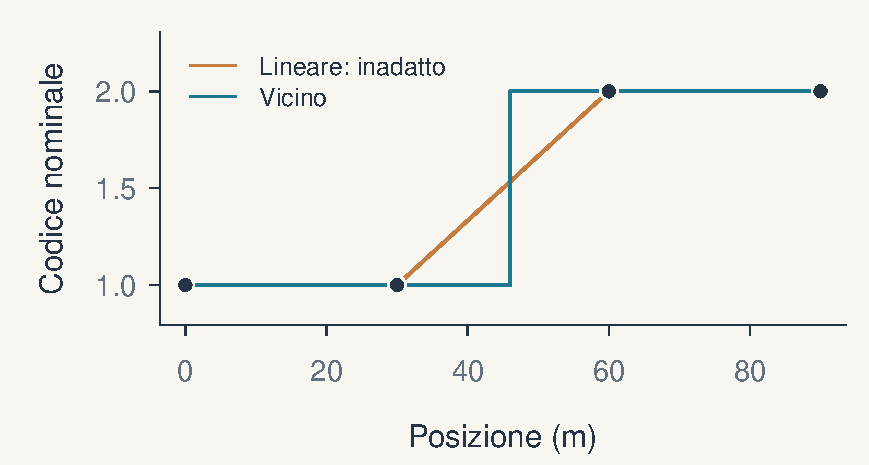
\includegraphics[width=9.85cm,height=5.25cm,keepaspectratio]{Risultati/Figure/13_ricampionamento_classi.pdf}
\vspace{1.5mm}
\PSmall{Le categorie 1 e 2 rappresentano classi nominali. Il valore interpolato 1,5 non identifica una terza classe valida.}

\end{minipage}\end{lrbox}
\typeout{FULLBOX:041:PilotLeftBox:\the\ht\PilotLeftBox:\the\dp\PilotLeftBox}

\begin{lrbox}{\PilotRightBox}
\begin{minipage}[t]{7.55cm}\raggedright\color{Ink}\fontsize{11.3}{14.8}\selectfont
\PBody{Una carta litologica richiede una regola che conservi il significato delle categorie, come il vicino più prossimo o una sintesi modale dichiarata.}
\vspace{2.5mm}
\PInfo{Il risultato dipende anche dalle regole di pareggio e dalla posizione dei confini rispetto alle celle.}
\PBody{Il fatto che i codici siano numerici non autorizza a trattarli come una scala quantitativa.}
\vspace{2.5mm}

\end{minipage}\end{lrbox}
\typeout{FULLBOX:041:PilotRightBox:\the\ht\PilotRightBox:\the\dp\PilotRightBox}

\begin{tikzpicture}[remember picture,overlay]
\PilotChrome{Le categorie richiedono regole proprie}{IV · RISOLUZIONE E ALLINEAMENTO}{41}{La scelta del metodo segue il significato della variabile, non il formato numerico della colonna.}
\node[anchor=north west,inner sep=0] at([xshift=.96cm,yshift=-2.13cm]current page.north west){\usebox{\PilotLeftBox}};
\node[anchor=north west,inner sep=0] at([xshift=11.52cm,yshift=-2.13cm]current page.north west){\usebox{\PilotRightBox}};
\node[anchor=north east,inner sep=0] at([xshift=17.65cm,yshift=-12.06cm]current page.north west){\color{Classical}\fontsize{7.7}{9.2}\selectfont\href{../../03_Notebook_svolti/M12_Tessera/M12_N08.html}{M12\_N08 · notebook svolto}};
\end{tikzpicture}\end{frame}

\begin{frame}[plain]\hypertarget{slide42}{}
\bookmark[level=1,page=42]{Quale proprietà deve conservarsi?}
\begin{lrbox}{\TitleBox}
\begin{minipage}[t]{17.7cm}\raggedright\color{Ink}\fontsize{11.3}{14.8}\selectfont
\color{Navy}\bfseries\fontsize{20.6}{24.5}\selectfont Quale proprietà deve conservarsi?
\end{minipage}\end{lrbox}
\typeout{FULLBOX:042:TitleBox:\the\ht\TitleBox:\the\dp\TitleBox}

\begin{lrbox}{\RecallBox}
\begin{minipage}[t]{14.3cm}\raggedright\color{Ink}\fontsize{11.3}{14.8}\selectfont
\fontsize{10.3}{13.8}\selectfont Un controllo di conservazione deve essere scelto in funzione della quantità scientifica.
\end{minipage}\end{lrbox}
\typeout{FULLBOX:042:RecallBox:\the\ht\RecallBox:\the\dp\RecallBox}

\begin{lrbox}{\PilotLeftBox}
\begin{minipage}[t]{10.05cm}\raggedright\color{Ink}\fontsize{11.3}{14.8}\selectfont
{\fontsize{10.2}{13.1}\selectfont\renewcommand{\arraystretch}{1.45}\begin{tabular}{@{}p{4.0cm}p{5.0cm}@{}}\toprule
\textbf{Variabile} & \textbf{Domanda da verificare}\\\midrule
Quota o temperatura & La regola ricostruisce una grandezza continua?\\
Quantità totale per cella & La somma si conserva sul dominio?\\
Densità per unità di area & Il peso considera l’area rappresentata?\\
Categoria nominale & I codici restano appartenenti alle classi?\\
Maschera di validità & Che cosa rende valida una cella di uscita?\\
\bottomrule\end{tabular}}

\end{minipage}\end{lrbox}
\typeout{FULLBOX:042:PilotLeftBox:\the\ht\PilotLeftBox:\the\dp\PilotLeftBox}

\begin{lrbox}{\PilotRightBox}
\begin{minipage}[t]{7.55cm}\raggedright\color{Ink}\fontsize{11.3}{14.8}\selectfont
\PBody{Una media è adatta a riassumere alcuni campi intensivi. Una quantità totale per cella richiede di considerare come viene distribuita o sommata.}
\vspace{2.5mm}
\PInfo{Prima dell’operazione scegliamo una proprietà controllabile: media, somma, intervallo, appartenenza o copertura.}
\PBody{La stessa procedura non conserva automaticamente tutte queste proprietà.}
\vspace{2.5mm}

\end{minipage}\end{lrbox}
\typeout{FULLBOX:042:PilotRightBox:\the\ht\PilotRightBox:\the\dp\PilotRightBox}

\begin{tikzpicture}[remember picture,overlay]
\PilotChrome{Quale proprietà deve conservarsi?}{IV · RISOLUZIONE E ALLINEAMENTO}{42}{Un controllo di conservazione deve essere scelto in funzione della quantità scientifica.}
\node[anchor=north west,inner sep=0] at([xshift=.96cm,yshift=-2.13cm]current page.north west){\usebox{\PilotLeftBox}};
\node[anchor=north west,inner sep=0] at([xshift=11.52cm,yshift=-2.13cm]current page.north west){\usebox{\PilotRightBox}};
\end{tikzpicture}\end{frame}

\begin{frame}[plain]\hypertarget{slide43}{}
\bookmark[level=1,page=43]{Stessa forma della matrice, origine diversa}
\begin{lrbox}{\TitleBox}
\begin{minipage}[t]{17.7cm}\raggedright\color{Ink}\fontsize{11.3}{14.8}\selectfont
\color{Navy}\bfseries\fontsize{20.6}{24.5}\selectfont Stessa forma della matrice, origine diversa
\end{minipage}\end{lrbox}
\typeout{FULLBOX:043:TitleBox:\the\ht\TitleBox:\the\dp\TitleBox}

\begin{lrbox}{\RecallBox}
\begin{minipage}[t]{14.3cm}\raggedright\color{Ink}\fontsize{11.3}{14.8}\selectfont
\fontsize{10.3}{13.8}\selectfont La compatibilità degli array deve essere verificata anche nella geometria territoriale.
\end{minipage}\end{lrbox}
\typeout{FULLBOX:043:RecallBox:\the\ht\RecallBox:\the\dp\RecallBox}

\begin{lrbox}{\PilotLeftBox}
\begin{minipage}[t]{10.05cm}\raggedright\color{Ink}\fontsize{11.3}{14.8}\selectfont
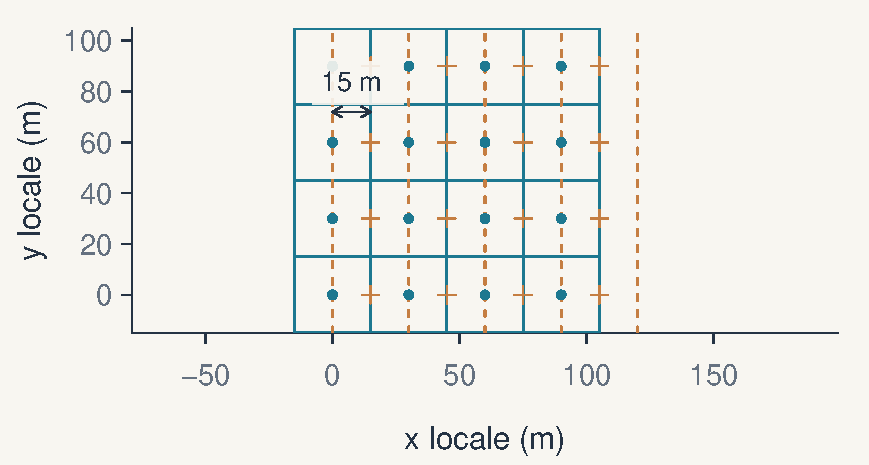
\includegraphics[width=9.85cm,height=5.25cm,keepaspectratio]{Risultati/Figure/14_origini_15m.pdf}
\vspace{1.5mm}
\PSmall{Due griglie di passo 30 m traslate di 15 m lungo Est. Le dimensioni delle matrici coincidono; i centri no.}

\end{minipage}\end{lrbox}
\typeout{FULLBOX:043:PilotLeftBox:\the\ht\PilotLeftBox:\the\dp\PilotLeftBox}

\begin{lrbox}{\PilotRightBox}
\begin{minipage}[t]{7.55cm}\raggedright\color{Ink}\fontsize{11.3}{14.8}\selectfont
\PBody{Una sottrazione per indice associa luoghi differenti. Il problema può restare poco visibile quando il campo varia gradualmente.}
\vspace{2.5mm}
\PInfo{Prima di combinare bande o epoche confrontiamo CRS, estensione, risoluzione e origine.}
\PCode{R · spostamento in pixel}{043_esempio.R}
\end{minipage}\end{lrbox}
\typeout{FULLBOX:043:PilotRightBox:\the\ht\PilotRightBox:\the\dp\PilotRightBox}

\begin{tikzpicture}[remember picture,overlay]
\PilotChrome{Stessa forma della matrice, origine diversa}{IV · RISOLUZIONE E ALLINEAMENTO}{43}{La compatibilità degli array deve essere verificata anche nella geometria territoriale.}
\node[anchor=north west,inner sep=0] at([xshift=.96cm,yshift=-2.13cm]current page.north west){\usebox{\PilotLeftBox}};
\node[anchor=north west,inner sep=0] at([xshift=11.52cm,yshift=-2.13cm]current page.north west){\usebox{\PilotRightBox}};
\node[anchor=north east,inner sep=0] at([xshift=17.65cm,yshift=-12.06cm]current page.north west){\color{Classical}\fontsize{7.7}{9.2}\selectfont\href{../../03_Notebook_svolti/M12_Tessera/M12_N19.html}{M12\_N19 · notebook svolto}};
\end{tikzpicture}\end{frame}

\begin{frame}[plain]\hypertarget{slide44}{}
\bookmark[level=1,page=44]{La griglia obiettivo rende esplicito l’allineamento}
\begin{lrbox}{\TitleBox}
\begin{minipage}[t]{17.7cm}\raggedright\color{Ink}\fontsize{11.3}{14.8}\selectfont
\color{Navy}\bfseries\fontsize{20.6}{24.5}\selectfont La griglia obiettivo rende esplicito l’allineamento
\end{minipage}\end{lrbox}
\typeout{FULLBOX:044:TitleBox:\the\ht\TitleBox:\the\dp\TitleBox}

\begin{lrbox}{\RecallBox}
\begin{minipage}[t]{14.3cm}\raggedright\color{Ink}\fontsize{11.3}{14.8}\selectfont
\fontsize{10.3}{13.8}\selectfont Una griglia comune è una decisione del progetto che deve poter essere ricostruita.
\end{minipage}\end{lrbox}
\typeout{FULLBOX:044:RecallBox:\the\ht\RecallBox:\the\dp\RecallBox}

\begin{lrbox}{\PilotLeftBox}
\begin{minipage}[t]{10.05cm}\raggedright\color{Ink}\fontsize{11.3}{14.8}\selectfont
\begin{tikzpicture}[x=1cm,y=1cm]
\path[use as bounding box](-.1,-.15) rectangle(9.7,4.8);
\node[pFlow,text width=3.7cm,fill=GeoA!7] (a) at(2.1,3.8){Raster da trasformare};
\node[pFlow,text width=3.7cm,fill=GeoB!7] (b) at(7.3,3.8){Griglia obiettivo dichiarata};
\node[pFlow,text width=3.7cm,fill=GeoC!7] (c) at(2.1,1.2){Metodo coerente con i valori};
\node[pFlow,text width=3.7cm,fill=GeoA!7] (d) at(7.3,1.2){Valori e geometria verificati};
\draw[pEdge] (a) -- (c);
\draw[pEdge] (b) -- (d);
\draw[pEdge] (c) -- (d);
\end{tikzpicture}

\end{minipage}\end{lrbox}
\typeout{FULLBOX:044:PilotLeftBox:\the\ht\PilotLeftBox:\the\dp\PilotLeftBox}

\begin{lrbox}{\PilotRightBox}
\begin{minipage}[t]{7.55cm}\raggedright\color{Ink}\fontsize{11.3}{14.8}\selectfont
\PBody{Il ricampionamento trasferisce i valori sulla geometria del modello di riferimento. Se cambia il CRS, occorre una riproiezione.}
\vspace{2.5mm}
\PInfo{Conserviamo la griglia obiettivo nel progetto. Controlliamo anche maschere e significato dei valori.}
\PCode{R · allineare una griglia}{044_esempio.R}
\end{minipage}\end{lrbox}
\typeout{FULLBOX:044:PilotRightBox:\the\ht\PilotRightBox:\the\dp\PilotRightBox}

\begin{tikzpicture}[remember picture,overlay]
\PilotChrome{La griglia obiettivo rende esplicito l’allineamento}{IV · RISOLUZIONE E ALLINEAMENTO}{44}{Una griglia comune è una decisione del progetto che deve poter essere ricostruita.}
\node[anchor=north west,inner sep=0] at([xshift=.96cm,yshift=-2.13cm]current page.north west){\usebox{\PilotLeftBox}};
\node[anchor=north west,inner sep=0] at([xshift=11.52cm,yshift=-2.13cm]current page.north west){\usebox{\PilotRightBox}};
\node[anchor=north east,inner sep=0] at([xshift=17.65cm,yshift=-12.06cm]current page.north west){\color{Classical}\fontsize{7.7}{9.2}\selectfont\href{../../03_Notebook_svolti/M12_Tessera/M12_N19.html}{M12\_N19 · notebook svolto}};
\end{tikzpicture}\end{frame}

\begin{frame}[plain]\hypertarget{slide45}{}
\bookmark[level=1,page=45]{Lo scarto prodotto da mezzo pixel}
\begin{lrbox}{\TitleBox}
\begin{minipage}[t]{17.7cm}\raggedright\color{Ink}\fontsize{11.3}{14.8}\selectfont
\color{Navy}\bfseries\fontsize{20.6}{24.5}\selectfont Lo scarto prodotto da mezzo pixel
\end{minipage}\end{lrbox}
\typeout{FULLBOX:045:TitleBox:\the\ht\TitleBox:\the\dp\TitleBox}

\begin{lrbox}{\RecallBox}
\begin{minipage}[t]{14.3cm}\raggedright\color{Ink}\fontsize{11.3}{14.8}\selectfont
\fontsize{10.3}{13.8}\selectfont La verifica geometrica viene prima dell’interpretazione delle mappe di cambiamento.
\end{minipage}\end{lrbox}
\typeout{FULLBOX:045:RecallBox:\the\ht\RecallBox:\the\dp\RecallBox}

\begin{lrbox}{\PilotLeftBox}
\begin{minipage}[t]{10.05cm}\raggedright\color{Ink}\fontsize{11.3}{14.8}\selectfont
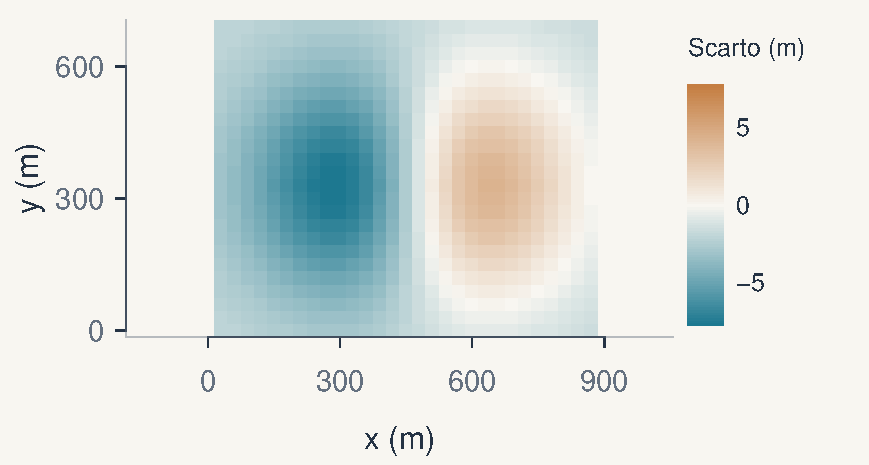
\includegraphics[width=9.85cm,height=4.4cm,keepaspectratio]{Risultati/Figure/15_allineamento_errori.pdf}
\vspace{1.5mm}
\PSmall{Stessi valori attribuiti a una griglia spostata di 15 m verso Est e poi riallineati: scarto dalla superficie originale.}
\[f(x-\delta,y)-f(x,y)\approx-\delta\,f_x(x,y)\]

\end{minipage}\end{lrbox}
\typeout{FULLBOX:045:PilotLeftBox:\the\ht\PilotLeftBox:\the\dp\PilotLeftBox}

\begin{lrbox}{\PilotRightBox}
\begin{minipage}[t]{7.55cm}\raggedright\color{Ink}\fontsize{11.3}{14.8}\selectfont
\PBody{Spostare la georeferenziazione dei valori verso Est costruisce un campo traslato. La differenza può derivare dalla geometria anziché da un cambiamento del terreno.}
\vspace{2.5mm}
\PInfo{Sul piano $f=ax+by+c$ lo scarto interno è $-a\delta$. Vicino ai bordi intervengono anche le regole del ricampionamento.}
\PCode{R · effetto noto della traslazione}{045_esempio.R}
\end{minipage}\end{lrbox}
\typeout{FULLBOX:045:PilotRightBox:\the\ht\PilotRightBox:\the\dp\PilotRightBox}

\begin{tikzpicture}[remember picture,overlay]
\PilotChrome{Lo scarto prodotto da mezzo pixel}{IV · RISOLUZIONE E ALLINEAMENTO}{45}{La verifica geometrica viene prima dell’interpretazione delle mappe di cambiamento.}
\node[anchor=north west,inner sep=0] at([xshift=.96cm,yshift=-2.13cm]current page.north west){\usebox{\PilotLeftBox}};
\node[anchor=north west,inner sep=0] at([xshift=11.52cm,yshift=-2.13cm]current page.north west){\usebox{\PilotRightBox}};
\node[anchor=north east,inner sep=0] at([xshift=17.65cm,yshift=-12.06cm]current page.north west){\color{Classical}\fontsize{7.7}{9.2}\selectfont\href{../../03_Notebook_svolti/M12_Tessera/M12_N19.html}{M12\_N19 · notebook svolto}};
\end{tikzpicture}\end{frame}

\begin{frame}[plain]\hypertarget{slide46}{}
\bookmark[level=1,page=46]{Il passo cambia il campionamento}
\begin{lrbox}{\TitleBox}
\begin{minipage}[t]{17.7cm}\raggedright\color{Ink}\fontsize{11.3}{14.8}\selectfont
\color{Navy}\bfseries\fontsize{20.6}{24.5}\selectfont Il passo cambia il campionamento
\end{minipage}\end{lrbox}
\typeout{FULLBOX:046:TitleBox:\the\ht\TitleBox:\the\dp\TitleBox}

\begin{lrbox}{\RecallBox}
\begin{minipage}[t]{14.3cm}\raggedright\color{Ink}\fontsize{11.3}{14.8}\selectfont
\fontsize{10.3}{13.8}\selectfont Per isolare l’effetto della risoluzione manteniamo fissi campo, dominio e regola di campionamento.
\end{minipage}\end{lrbox}
\typeout{FULLBOX:046:RecallBox:\the\ht\RecallBox:\the\dp\RecallBox}

\begin{lrbox}{\FullWideBox}
\begin{minipage}[t]{18.1cm}\raggedright\color{Ink}\fontsize{11.3}{14.8}\selectfont
\centering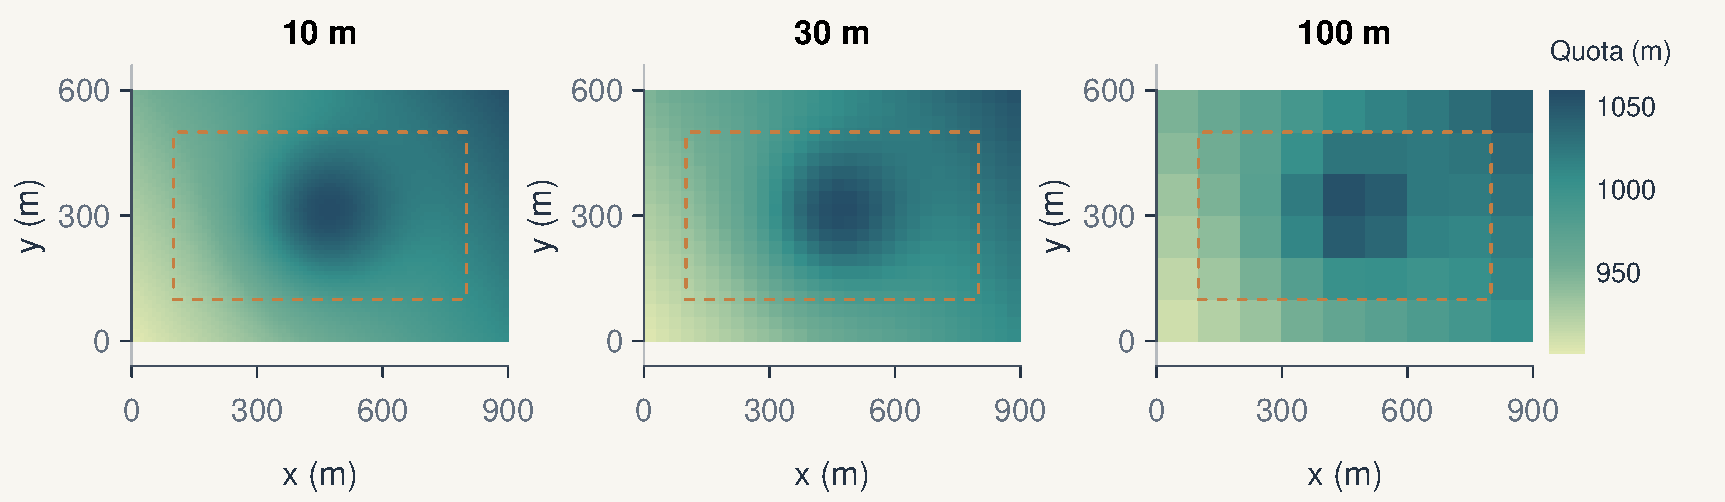
\includegraphics[width=18.05cm,height=5.8cm,keepaspectratio]{Risultati/Figure/10_risoluzioni_analitiche.pdf}
\end{minipage}\end{lrbox}
\typeout{FULLBOX:046:FullWideBox:\the\ht\FullWideBox:\the\dp\FullWideBox}

\begin{lrbox}{\PilotRightBox}
\begin{minipage}[t]{18.1cm}\raggedright\color{Ink}\fontsize{11.3}{14.8}\selectfont
\PBody{Esperimento analitico separato dal raster originale: stesso campo e dominio di 900×600 m, griglie di 10, 30 e 100 m. I valori sono valutati secondo la regola documentata nel codice; non sono nuove misure del terreno del corso. La scala cromatica comune rende confrontabile il dettaglio rappresentato.}
\end{minipage}\end{lrbox}
\typeout{FULLBOX:046:PilotRightBox:\the\ht\PilotRightBox:\the\dp\PilotRightBox}

\begin{tikzpicture}[remember picture,overlay]
\PilotChrome{Il passo cambia il campionamento}{IV · RISOLUZIONE E ALLINEAMENTO}{46}{Per isolare l’effetto della risoluzione manteniamo fissi campo, dominio e regola di campionamento.}
\node[anchor=north west,inner sep=0] at([xshift=.96cm,yshift=-2.13cm]current page.north west){\usebox{\FullWideBox}};
\node[anchor=north west,inner sep=0] at([xshift=.96cm,yshift=-8.25cm]current page.north west){\usebox{\PilotRightBox}};
\end{tikzpicture}\end{frame}

\begin{frame}[plain]\hypertarget{slide47}{}
\bookmark[level=1,page=47]{Prima aggregare o prima derivare?}
\begin{lrbox}{\TitleBox}
\begin{minipage}[t]{17.7cm}\raggedright\color{Ink}\fontsize{11.3}{14.8}\selectfont
\color{Navy}\bfseries\fontsize{20.6}{24.5}\selectfont Prima aggregare o prima derivare?
\end{minipage}\end{lrbox}
\typeout{FULLBOX:047:TitleBox:\the\ht\TitleBox:\the\dp\TitleBox}

\begin{lrbox}{\RecallBox}
\begin{minipage}[t]{14.3cm}\raggedright\color{Ink}\fontsize{11.3}{14.8}\selectfont
\fontsize{10.3}{13.8}\selectfont Il metodo deve specificare sia l’operazione sia l’ordine in cui viene applicata.
\end{minipage}\end{lrbox}
\typeout{FULLBOX:047:RecallBox:\the\ht\RecallBox:\the\dp\RecallBox}

\begin{lrbox}{\PilotLeftBox}
\begin{minipage}[t]{10.05cm}\raggedright\color{Ink}\fontsize{11.3}{14.8}\selectfont
\begin{tikzpicture}[x=1cm,y=1cm]
\path[use as bounding box](-.1,-.15) rectangle(9.7,4.8);
\node[pFlow,text width=3.7cm,fill=GeoA!7] (a) at(2.1,3.8){Quote a 30 m};
\node[pFlow,text width=3.7cm,fill=GeoB!7] (b) at(7.3,3.8){Medie delle quote a 60 m};
\node[pFlow,text width=3.7cm,fill=GeoA!7] (c) at(2.1,1.2){Pendenze a 30 m, poi media};
\node[pFlow,text width=3.7cm,fill=GeoB!7] (d) at(7.3,1.2){Pendenze calcolate a 60 m};
\draw[pEdge] (a) -- (b);
\draw[pEdge] (a) -- (c);
\draw[pEdge] (b) -- (d);
\end{tikzpicture}
\[\overline{\alpha(z_{30})}\ \ne\
       \alpha(\overline z_{60})\quad\text{in generale}\]

\end{minipage}\end{lrbox}
\typeout{FULLBOX:047:PilotLeftBox:\the\ht\PilotLeftBox:\the\dp\PilotLeftBox}

\begin{lrbox}{\PilotRightBox}
\begin{minipage}[t]{7.55cm}\raggedright\color{Ink}\fontsize{11.3}{14.8}\selectfont
\PBody{Una derivata calcolata dopo l’aggregazione usa un campo più liscio e un passo diverso. La media di pendenze già calcolate riassume invece una grandezza non lineare.}
\vspace{2.5mm}
\PInfo{Non assumiamo l’uguaglianza dei due risultati. Li confrontiamo sul dominio valido comune, considerando anche i bordi.}
\PBody{La scala del DEM deve accompagnare la carta delle pendenze e ogni confronto fra prodotti.}
\vspace{2.5mm}

\end{minipage}\end{lrbox}
\typeout{FULLBOX:047:PilotRightBox:\the\ht\PilotRightBox:\the\dp\PilotRightBox}

\begin{tikzpicture}[remember picture,overlay]
\PilotChrome{Prima aggregare o prima derivare?}{IV · RISOLUZIONE E ALLINEAMENTO}{47}{Il metodo deve specificare sia l’operazione sia l’ordine in cui viene applicata.}
\node[anchor=north west,inner sep=0] at([xshift=.96cm,yshift=-2.13cm]current page.north west){\usebox{\PilotLeftBox}};
\node[anchor=north west,inner sep=0] at([xshift=11.52cm,yshift=-2.13cm]current page.north west){\usebox{\PilotRightBox}};
\node[anchor=north east,inner sep=0] at([xshift=17.65cm,yshift=-12.06cm]current page.north west){\color{Classical}\fontsize{7.7}{9.2}\selectfont\href{../../03_Notebook_svolti/M12_Tessera/M12_N07.html}{M12\_N07 · notebook svolto}};
\end{tikzpicture}\end{frame}

\begin{frame}[plain]\hypertarget{slide48}{}
\bookmark[level=1,page=48]{Laboratorio: trasformare la griglia con un controllo}
\begin{lrbox}{\TitleBox}
\begin{minipage}[t]{17.7cm}\raggedright\color{Ink}\fontsize{11.3}{14.8}\selectfont
\color{Navy}\bfseries\fontsize{20.6}{24.5}\selectfont Laboratorio: trasformare la griglia con un controllo
\end{minipage}\end{lrbox}
\typeout{FULLBOX:048:TitleBox:\the\ht\TitleBox:\the\dp\TitleBox}

\begin{lrbox}{\RecallBox}
\begin{minipage}[t]{14.3cm}\raggedright\color{Ink}\fontsize{11.3}{14.8}\selectfont
\fontsize{10.3}{13.8}\selectfont La trasformazione è riuscita quando valori, geometria e proprietà attese risultano coerenti.
\end{minipage}\end{lrbox}
\typeout{FULLBOX:048:RecallBox:\the\ht\RecallBox:\the\dp\RecallBox}

\begin{lrbox}{\PilotLeftBox}
\begin{minipage}[t]{10.05cm}\raggedright\color{Ink}\fontsize{11.3}{14.8}\selectfont
\PLab{https://marzione00.github.io/Lab_Geo/\#laboratorio/m12-ricampionamento}{Esperimento online · aggregare e ricampionare}
\PLab{https://marzione00.github.io/Lab_Geo/\#laboratorio/m12-allineamento}{Esperimento online · allineamento}
{\fontsize{10.2}{13.1}\selectfont\renewcommand{\arraystretch}{1.45}\begin{tabular}{@{}p{4.2cm}p{4.8cm}@{}}\toprule
\textbf{Attività} & \textbf{Verifica}\\\midrule
N07: aggregazione & 180 blocchi completi, media conservata\\
N08: metodo & Quote continue e categorie distinte\\
N19: origine & Traslazione di mezzo pixel riconosciuta\\
Approfondimento & Risoluzioni 10, 30 e 100 m\\
Consegna & Geometria obiettivo, metodo e maschere\\
\bottomrule\end{tabular}}

\end{minipage}\end{lrbox}
\typeout{FULLBOX:048:PilotLeftBox:\the\ht\PilotLeftBox:\the\dp\PilotLeftBox}

\begin{lrbox}{\PilotRightBox}
\begin{minipage}[t]{7.55cm}\raggedright\color{Ink}\fontsize{11.3}{14.8}\selectfont
\PBody{La trasformazione deve produrre un oggetto interpretabile e controllabile. Una figura più gradevole non basta a stabilire la qualità del dato.}
\vspace{2.5mm}
\PInfo{Le prossime sezioni useranno la griglia originale da 30 m per le differenze centrate, salvo esperimenti di sensibilità esplicitamente indicati.}

\end{minipage}\end{lrbox}
\typeout{FULLBOX:048:PilotRightBox:\the\ht\PilotRightBox:\the\dp\PilotRightBox}

\begin{tikzpicture}[remember picture,overlay]
\PilotChrome{Laboratorio: trasformare la griglia con un controllo}{IV · RISOLUZIONE E ALLINEAMENTO}{48}{La trasformazione è riuscita quando valori, geometria e proprietà attese risultano coerenti.}
\node[anchor=north west,inner sep=0] at([xshift=.96cm,yshift=-2.13cm]current page.north west){\usebox{\PilotLeftBox}};
\node[anchor=north west,inner sep=0] at([xshift=11.52cm,yshift=-2.13cm]current page.north west){\usebox{\PilotRightBox}};
\node[anchor=north east,inner sep=0] at([xshift=17.65cm,yshift=-12.06cm]current page.north west){\color{Classical}\fontsize{7.7}{9.2}\selectfont\href{../../03_Notebook_svolti/M12_Tessera/M12_N19.html}{M12\_N19 · notebook svolto}};
\end{tikzpicture}\end{frame}

\begin{frame}[plain]\hypertarget{slide49}{}
\bookmark[level=0,page=49]{V · MORFOMETRIA}
\bookmark[level=1,page=49]{La morfometria deriva misure dalla geometria}
\begin{lrbox}{\TitleBox}
\begin{minipage}[t]{17.7cm}\raggedright\color{Ink}\fontsize{11.3}{14.8}\selectfont
\color{Navy}\bfseries\fontsize{20.6}{24.5}\selectfont La morfometria deriva misure dalla geometria
\end{minipage}\end{lrbox}
\typeout{FULLBOX:049:TitleBox:\the\ht\TitleBox:\the\dp\TitleBox}

\begin{lrbox}{\RecallBox}
\begin{minipage}[t]{14.3cm}\raggedright\color{Ink}\fontsize{11.3}{14.8}\selectfont
\fontsize{10.3}{13.8}\selectfont Una misura morfometrica è il risultato di dati geometrici e di un procedimento dichiarato.
\end{minipage}\end{lrbox}
\typeout{FULLBOX:049:RecallBox:\the\ht\RecallBox:\the\dp\RecallBox}

\begin{lrbox}{\PilotLeftBox}
\begin{minipage}[t]{10.05cm}\raggedright\color{Ink}\fontsize{11.3}{14.8}\selectfont
{\fontsize{10.2}{13.1}\selectfont\renewcommand{\arraystretch}{1.45}\begin{tabular}{@{}p{3.8cm}p{5.2cm}@{}}\toprule
\textbf{Grandezza} & \textbf{Domanda}\\\midrule
Quota & Quanto è alta la superficie nel riferimento?\\
Gradiente & Come cambia la quota lungo gli assi?\\
Pendenza & Qual è la massima inclinazione locale?\\
Esposizione & Verso quale azimut scende il terreno?\\
Ombreggiatura & Come appare con una luce scelta?\\
\bottomrule\end{tabular}}

\end{minipage}\end{lrbox}
\typeout{FULLBOX:049:PilotLeftBox:\the\ht\PilotLeftBox:\the\dp\PilotLeftBox}

\begin{lrbox}{\PilotRightBox}
\begin{minipage}[t]{7.55cm}\raggedright\color{Ink}\fontsize{11.3}{14.8}\selectfont
\PBody{Il valore derivato dipende dalla superficie rappresentata e dalla regola numerica. La risoluzione entra attraverso le distanze fra celle.}
\vspace{2.5mm}
\PInfo{Useremo prima un piano con soluzione nota, poi il terreno sintetico del corso. Questo separa il controllo del codice dall’interpretazione della morfologia.}
\PBody{La carta finale conserverà algoritmo, unità, passo e trattamento dei margini.}
\vspace{2.5mm}

\end{minipage}\end{lrbox}
\typeout{FULLBOX:049:PilotRightBox:\the\ht\PilotRightBox:\the\dp\PilotRightBox}

\begin{tikzpicture}[remember picture,overlay]
\PilotChrome{La morfometria deriva misure dalla geometria}{V · MORFOMETRIA}{49}{Una misura morfometrica è il risultato di dati geometrici e di un procedimento dichiarato.}
\node[anchor=north west,inner sep=0] at([xshift=.96cm,yshift=-2.13cm]current page.north west){\usebox{\PilotLeftBox}};
\node[anchor=north west,inner sep=0] at([xshift=11.52cm,yshift=-2.13cm]current page.north west){\usebox{\PilotRightBox}};
\end{tikzpicture}\end{frame}

\begin{frame}[plain]\hypertarget{slide50}{}
\bookmark[level=1,page=50]{Il gradiente misura variazioni orientate della quota}
\begin{lrbox}{\TitleBox}
\begin{minipage}[t]{17.7cm}\raggedright\color{Ink}\fontsize{11.3}{14.8}\selectfont
\color{Navy}\bfseries\fontsize{20.6}{24.5}\selectfont Il gradiente misura variazioni orientate della quota
\end{minipage}\end{lrbox}
\typeout{FULLBOX:050:TitleBox:\the\ht\TitleBox:\the\dp\TitleBox}

\begin{lrbox}{\RecallBox}
\begin{minipage}[t]{14.3cm}\raggedright\color{Ink}\fontsize{11.3}{14.8}\selectfont
\fontsize{10.3}{13.8}\selectfont Il gradiente deve essere interpretato insieme agli assi e alle loro unità.
\end{minipage}\end{lrbox}
\typeout{FULLBOX:050:RecallBox:\the\ht\RecallBox:\the\dp\RecallBox}

\begin{lrbox}{\PilotLeftBox}
\begin{minipage}[t]{10.05cm}\raggedright\color{Ink}\fontsize{11.3}{14.8}\selectfont
\begin{tikzpicture}[x=1cm,y=1cm]
\path[use as bounding box](-.1,-.15) rectangle(9.7,5.3);
\filldraw[fill=GeoA!9,draw=Rule](2.1,0.6)rectangle(3.6500000000000004,2.0);
\filldraw[fill=GeoA!9,draw=Rule](3.6500000000000004,0.6)rectangle(5.2,2.0);
\filldraw[fill=GeoA!9,draw=Rule](5.2,0.6)rectangle(6.75,2.0);
\filldraw[fill=GeoA!9,draw=Rule](2.1,2.0)rectangle(3.6500000000000004,3.4);
\filldraw[fill=GeoB!18,draw=Rule](3.6500000000000004,2.0)rectangle(5.2,3.4);
\filldraw[fill=GeoA!9,draw=Rule](5.2,2.0)rectangle(6.75,3.4);
\filldraw[fill=GeoA!9,draw=Rule](2.1,3.4)rectangle(3.6500000000000004,4.8);
\filldraw[fill=GeoA!9,draw=Rule](3.6500000000000004,3.4)rectangle(5.2,4.8);
\filldraw[fill=GeoA!9,draw=Rule](5.2,3.4)rectangle(6.75,4.8);
\node[pLabel]at(4.425,2.7){$z_{ij}$};
\node[pLabel]at(5.975,2.7){$z_{i,j+1}$};
\node[pLabel]at(2.875,2.7){$z_{i,j-1}$};
\node[pLabel]at(4.425,4.1){$z_{i+1,j}$};
\node[pLabel]at(4.425,1.3){$z_{i-1,j}$};
\draw[pEdge](7.1,1)--(7.1,4.6)node[above,pNote]{Nord};
\draw[<->,Muted](2.875,.2)--node[below,pNote]{$2\Delta x$}(5.975,.2);
\end{tikzpicture}
\[\nabla z=\left(\frac{\partial z}{\partial x},
                       \frac{\partial z}{\partial y}\right)\]

\end{minipage}\end{lrbox}
\typeout{FULLBOX:050:PilotLeftBox:\the\ht\PilotLeftBox:\the\dp\PilotLeftBox}

\begin{lrbox}{\PilotRightBox}
\begin{minipage}[t]{7.55cm}\raggedright\color{Ink}\fontsize{11.3}{14.8}\selectfont
\PBody{La componente lungo Est descrive come cambia la quota muovendosi su quell’asse. La componente lungo Nord usa l’orientamento geografico corrispondente.}
\vspace{2.5mm}
\PInfo{Il segno contiene informazione: una componente positiva indica salita nella direzione positiva dell’asse.}
\PBody{La norma del gradiente e la sua direzione descrivono proprietà diverse. La pendenza non conserva da sola l’esposizione.}
\vspace{2.5mm}

\end{minipage}\end{lrbox}
\typeout{FULLBOX:050:PilotRightBox:\the\ht\PilotRightBox:\the\dp\PilotRightBox}

\begin{tikzpicture}[remember picture,overlay]
\PilotChrome{Il gradiente misura variazioni orientate della quota}{V · MORFOMETRIA}{50}{Il gradiente deve essere interpretato insieme agli assi e alle loro unità.}
\node[anchor=north west,inner sep=0] at([xshift=.96cm,yshift=-2.13cm]current page.north west){\usebox{\PilotLeftBox}};
\node[anchor=north west,inner sep=0] at([xshift=11.52cm,yshift=-2.13cm]current page.north west){\usebox{\PilotRightBox}};
\end{tikzpicture}\end{frame}

\begin{frame}[plain]\hypertarget{slide51}{}
\bookmark[level=1,page=51]{Le differenze centrate usano due passi}
\begin{lrbox}{\TitleBox}
\begin{minipage}[t]{17.7cm}\raggedright\color{Ink}\fontsize{11.3}{14.8}\selectfont
\color{Navy}\bfseries\fontsize{20.6}{24.5}\selectfont Le differenze centrate usano due passi
\end{minipage}\end{lrbox}
\typeout{FULLBOX:051:TitleBox:\the\ht\TitleBox:\the\dp\TitleBox}

\begin{lrbox}{\RecallBox}
\begin{minipage}[t]{14.3cm}\raggedright\color{Ink}\fontsize{11.3}{14.8}\selectfont
\fontsize{10.3}{13.8}\selectfont Il denominatore è una distanza geometrica, non un parametro da scegliere per adattare il risultato.
\end{minipage}\end{lrbox}
\typeout{FULLBOX:051:RecallBox:\the\ht\RecallBox:\the\dp\RecallBox}

\begin{lrbox}{\PilotLeftBox}
\begin{minipage}[t]{10.05cm}\raggedright\color{Ink}\fontsize{11.3}{14.8}\selectfont
\[g_x=\frac{z_{i,j+1}-z_{i,j-1}}{2\Delta x}\]
\[g_y=\frac{z_{i+1,j}-z_{i-1,j}}{2\Delta y}\]
\PInfo{Matrice locale con righe crescenti verso Nord. Per $\Delta x=\Delta y=30$ m il denominatore è 60 m.}

\end{minipage}\end{lrbox}
\typeout{FULLBOX:051:PilotLeftBox:\the\ht\PilotLeftBox:\the\dp\PilotLeftBox}

\begin{lrbox}{\PilotRightBox}
\begin{minipage}[t]{7.55cm}\raggedright\color{Ink}\fontsize{11.3}{14.8}\selectfont
\PBody{I due valori confrontati si trovano ai lati del centro. La loro distanza è doppia rispetto al passo della griglia.}
\vspace{2.5mm}
\PSmall{Conserviamo soltanto le righe e colonne interne, dove entrambi i vicini sono disponibili.}
\PCode{R · derivate nella matrice locale}{051_esempio.R}
\end{minipage}\end{lrbox}
\typeout{FULLBOX:051:PilotRightBox:\the\ht\PilotRightBox:\the\dp\PilotRightBox}

\begin{tikzpicture}[remember picture,overlay]
\PilotChrome{Le differenze centrate usano due passi}{V · MORFOMETRIA}{51}{Il denominatore è una distanza geometrica, non un parametro da scegliere per adattare il risultato.}
\node[anchor=north west,inner sep=0] at([xshift=.96cm,yshift=-2.13cm]current page.north west){\usebox{\PilotLeftBox}};
\node[anchor=north west,inner sep=0] at([xshift=11.52cm,yshift=-2.13cm]current page.north west){\usebox{\PilotRightBox}};
\node[anchor=north east,inner sep=0] at([xshift=17.65cm,yshift=-12.06cm]current page.north west){\color{Classical}\fontsize{7.7}{9.2}\selectfont\href{../../03_Notebook_svolti/M12_Tessera/M12_N09.html}{M12\_N09 · notebook svolto}};
\end{tikzpicture}\end{frame}

\begin{frame}[plain]\hypertarget{slide52}{}
\bookmark[level=1,page=52]{Quote e distanze devono avere unità coerenti}
\begin{lrbox}{\TitleBox}
\begin{minipage}[t]{17.7cm}\raggedright\color{Ink}\fontsize{11.3}{14.8}\selectfont
\color{Navy}\bfseries\fontsize{20.6}{24.5}\selectfont Quote e distanze devono avere unità coerenti
\end{minipage}\end{lrbox}
\typeout{FULLBOX:052:TitleBox:\the\ht\TitleBox:\the\dp\TitleBox}

\begin{lrbox}{\RecallBox}
\begin{minipage}[t]{14.3cm}\raggedright\color{Ink}\fontsize{11.3}{14.8}\selectfont
\fontsize{10.3}{13.8}\selectfont L’unità della derivata deriva dalle unità dei dati, che devono essere verificate prima del calcolo.
\end{minipage}\end{lrbox}
\typeout{FULLBOX:052:RecallBox:\the\ht\RecallBox:\the\dp\RecallBox}

\begin{lrbox}{\PilotLeftBox}
\begin{minipage}[t]{10.05cm}\raggedright\color{Ink}\fontsize{11.3}{14.8}\selectfont
\[[g_x]=\frac{[\mathrm{quota}]}{[\mathrm{distanza}]}\]
{\fontsize{10.2}{13.1}\selectfont\renewcommand{\arraystretch}{1.45}\begin{tabular}{@{}p{4.2cm}p{4.8cm}@{}}\toprule
\textbf{Configurazione} & \textbf{Conseguenza}\\\midrule
Quota e assi in metri & Rapporto adimensionale\\
Quota in piedi, assi in metri & Conversione necessaria\\
Assi in gradi & Distanza metrica da ricostruire\\
Passi diversi su x e y & Denominatori distinti\\
Esagerazione verticale & Inclinazione rappresentata modificata\\
\bottomrule\end{tabular}}

\end{minipage}\end{lrbox}
\typeout{FULLBOX:052:PilotLeftBox:\the\ht\PilotLeftBox:\the\dp\PilotLeftBox}

\begin{lrbox}{\PilotRightBox}
\begin{minipage}[t]{7.55cm}\raggedright\color{Ink}\fontsize{11.3}{14.8}\selectfont
\PBody{La tangente dell’angolo di pendenza è un rapporto fra lunghezze espresse nella stessa unità.}
\vspace{2.5mm}
\PInfo{Il caso guida usa metri per quote e coordinate. Un DEM geografico richiede un algoritmo che tenga conto delle distanze sulla Terra.}
\PBody{Una trasformazione dei soli valori per migliorare la visualizzazione non deve entrare implicitamente nei calcoli scientifici.}
\vspace{2.5mm}

\end{minipage}\end{lrbox}
\typeout{FULLBOX:052:PilotRightBox:\the\ht\PilotRightBox:\the\dp\PilotRightBox}

\begin{tikzpicture}[remember picture,overlay]
\PilotChrome{Quote e distanze devono avere unità coerenti}{V · MORFOMETRIA}{52}{L’unità della derivata deriva dalle unità dei dati, che devono essere verificate prima del calcolo.}
\node[anchor=north west,inner sep=0] at([xshift=.96cm,yshift=-2.13cm]current page.north west){\usebox{\PilotLeftBox}};
\node[anchor=north west,inner sep=0] at([xshift=11.52cm,yshift=-2.13cm]current page.north west){\usebox{\PilotRightBox}};
\end{tikzpicture}\end{frame}

\begin{frame}[plain]\hypertarget{slide53}{}
\bookmark[level=1,page=53]{Un piano fornisce una soluzione di riferimento}
\begin{lrbox}{\TitleBox}
\begin{minipage}[t]{17.7cm}\raggedright\color{Ink}\fontsize{11.3}{14.8}\selectfont
\color{Navy}\bfseries\fontsize{20.6}{24.5}\selectfont Un piano fornisce una soluzione di riferimento
\end{minipage}\end{lrbox}
\typeout{FULLBOX:053:TitleBox:\the\ht\TitleBox:\the\dp\TitleBox}

\begin{lrbox}{\RecallBox}
\begin{minipage}[t]{14.3cm}\raggedright\color{Ink}\fontsize{11.3}{14.8}\selectfont
\fontsize{10.3}{13.8}\selectfont Una verifica utile confronta il codice con un risultato noto indipendentemente.
\end{minipage}\end{lrbox}
\typeout{FULLBOX:053:RecallBox:\the\ht\RecallBox:\the\dp\RecallBox}

\begin{lrbox}{\PilotLeftBox}
\begin{minipage}[t]{10.05cm}\raggedright\color{Ink}\fontsize{11.3}{14.8}\selectfont
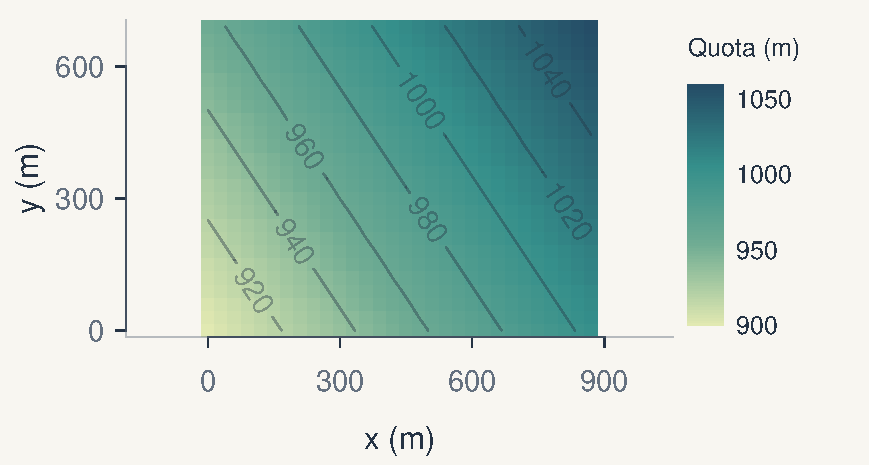
\includegraphics[width=9.85cm,height=5.25cm,keepaspectratio]{Risultati/Figure/16_piano_noto.pdf}
\vspace{1.5mm}
\PSmall{Piano sintetico $z=900+0{,}12x+0{,}08y$. Il gradiente esatto è noto in tutto il dominio.}

\end{minipage}\end{lrbox}
\typeout{FULLBOX:053:PilotLeftBox:\the\ht\PilotLeftBox:\the\dp\PilotLeftBox}

\begin{lrbox}{\PilotRightBox}
\begin{minipage}[t]{7.55cm}\raggedright\color{Ink}\fontsize{11.3}{14.8}\selectfont
\PBody{Le derivate sono costanti: 0,12 lungo Est e 0,08 lungo Nord. Il livello iniziale 900 m non cambia l’inclinazione.}
\vspace{2.5mm}
\PInfo{La soluzione analitica è disponibile prima di eseguire il programma. Può quindi riconoscere errori nel passo, nel segno o nell’ordine degli assi.}
\PCode{R · piano e pendenza attesa}{053_esempio.R}
\end{minipage}\end{lrbox}
\typeout{FULLBOX:053:PilotRightBox:\the\ht\PilotRightBox:\the\dp\PilotRightBox}

\begin{tikzpicture}[remember picture,overlay]
\PilotChrome{Un piano fornisce una soluzione di riferimento}{V · MORFOMETRIA}{53}{Una verifica utile confronta il codice con un risultato noto indipendentemente.}
\node[anchor=north west,inner sep=0] at([xshift=.96cm,yshift=-2.13cm]current page.north west){\usebox{\PilotLeftBox}};
\node[anchor=north west,inner sep=0] at([xshift=11.52cm,yshift=-2.13cm]current page.north west){\usebox{\PilotRightBox}};
\node[anchor=north east,inner sep=0] at([xshift=17.65cm,yshift=-12.06cm]current page.north west){\color{Classical}\fontsize{7.7}{9.2}\selectfont\href{../../03_Notebook_svolti/M12_Tessera/M12_N09.html}{M12\_N09 · notebook svolto}};
\end{tikzpicture}\end{frame}

\begin{frame}[plain]\hypertarget{slide54}{}
\bookmark[level=1,page=54]{Il controllo confronta entrambe le componenti}
\begin{lrbox}{\TitleBox}
\begin{minipage}[t]{17.7cm}\raggedright\color{Ink}\fontsize{11.3}{14.8}\selectfont
\color{Navy}\bfseries\fontsize{20.6}{24.5}\selectfont Il controllo confronta entrambe le componenti
\end{minipage}\end{lrbox}
\typeout{FULLBOX:054:TitleBox:\the\ht\TitleBox:\the\dp\TitleBox}

\begin{lrbox}{\RecallBox}
\begin{minipage}[t]{14.3cm}\raggedright\color{Ink}\fontsize{11.3}{14.8}\selectfont
\fontsize{10.3}{13.8}\selectfont Verificare soltanto la norma può nascondere un errore di direzione.
\end{minipage}\end{lrbox}
\typeout{FULLBOX:054:RecallBox:\the\ht\RecallBox:\the\dp\RecallBox}

\begin{lrbox}{\PilotLeftBox}
\begin{minipage}[t]{10.05cm}\raggedright\color{Ink}\fontsize{11.3}{14.8}\selectfont
\[\max|g_x-0{,}12|<10^{-12}\]
\[\max|g_y-0{,}08|<10^{-12}\]
\PInfo{La tolleranza riconosce l’aritmetica in virgola mobile. Il confronto riguarda tutte le celle interne, non soltanto la media.}

\end{minipage}\end{lrbox}
\typeout{FULLBOX:054:PilotLeftBox:\the\ht\PilotLeftBox:\the\dp\PilotLeftBox}

\begin{lrbox}{\PilotRightBox}
\begin{minipage}[t]{7.55cm}\raggedright\color{Ink}\fontsize{11.3}{14.8}\selectfont
\PBody{Un errore di orientamento può cambiare il segno della componente Nord lasciando invariata la norma del gradiente.}
\vspace{2.5mm}
\PSmall{Per questo controlliamo le componenti prima dell’angolo di pendenza.}
\PCode{R · prova numerica indipendente}{054_esempio.R}
\end{minipage}\end{lrbox}
\typeout{FULLBOX:054:PilotRightBox:\the\ht\PilotRightBox:\the\dp\PilotRightBox}

\begin{tikzpicture}[remember picture,overlay]
\PilotChrome{Il controllo confronta entrambe le componenti}{V · MORFOMETRIA}{54}{Verificare soltanto la norma può nascondere un errore di direzione.}
\node[anchor=north west,inner sep=0] at([xshift=.96cm,yshift=-2.13cm]current page.north west){\usebox{\PilotLeftBox}};
\node[anchor=north west,inner sep=0] at([xshift=11.52cm,yshift=-2.13cm]current page.north west){\usebox{\PilotRightBox}};
\node[anchor=north east,inner sep=0] at([xshift=17.65cm,yshift=-12.06cm]current page.north west){\color{Classical}\fontsize{7.7}{9.2}\selectfont\href{../../03_Notebook_svolti/M12_Tessera/M12_N09.html}{M12\_N09 · notebook svolto}};
\end{tikzpicture}\end{frame}

\begin{frame}[plain]\hypertarget{slide55}{}
\bookmark[level=1,page=55]{Gli errori costruiti mostrano che cosa controllare}
\begin{lrbox}{\TitleBox}
\begin{minipage}[t]{17.7cm}\raggedright\color{Ink}\fontsize{11.3}{14.8}\selectfont
\color{Navy}\bfseries\fontsize{20.6}{24.5}\selectfont Gli errori costruiti mostrano che cosa controllare
\end{minipage}\end{lrbox}
\typeout{FULLBOX:055:TitleBox:\the\ht\TitleBox:\the\dp\TitleBox}

\begin{lrbox}{\RecallBox}
\begin{minipage}[t]{14.3cm}\raggedright\color{Ink}\fontsize{11.3}{14.8}\selectfont
\fontsize{10.3}{13.8}\selectfont Le proprietà geometriche aiutano a progettare controlli che distinguono errori e cambiamenti legittimi.
\end{minipage}\end{lrbox}
\typeout{FULLBOX:055:RecallBox:\the\ht\RecallBox:\the\dp\RecallBox}

\begin{lrbox}{\PilotLeftBox}
\begin{minipage}[t]{10.05cm}\raggedright\color{Ink}\fontsize{11.3}{14.8}\selectfont
{\fontsize{10.2}{13.1}\selectfont\renewcommand{\arraystretch}{1.45}\begin{tabular}{@{}p{4.7cm}p{4.3cm}@{}}\toprule
\textbf{Errore introdotto} & \textbf{Effetto sul piano}\\\midrule
Usare $\Delta$ invece di $2\Delta$ & Componenti raddoppiate\\
Invertire Nord e Sud & Segno della componente Nord invertito\\
Scambiare gli assi & Componenti scambiate\\
Aggiungere una costante alle quote & Gradiente invariato\\
Moltiplicare le quote per un fattore & Gradiente moltiplicato per quel fattore\\
\bottomrule\end{tabular}}

\end{minipage}\end{lrbox}
\typeout{FULLBOX:055:PilotLeftBox:\the\ht\PilotLeftBox:\the\dp\PilotLeftBox}

\begin{lrbox}{\PilotRightBox}
\begin{minipage}[t]{7.55cm}\raggedright\color{Ink}\fontsize{11.3}{14.8}\selectfont
\PBody{Queste trasformazioni rendono esplicito il comportamento atteso. Una verifica deve fallire quando introduciamo un errore che pretende di riconoscere.}
\vspace{2.5mm}
\PInfo{L’angolo è l’arcotangente della norma: raddoppiare il gradiente non raddoppia esattamente l’angolo.}
\PBody{Una volta superate le prove note, applichiamo il calcolo al rilievo articolato.}
\vspace{2.5mm}

\end{minipage}\end{lrbox}
\typeout{FULLBOX:055:PilotRightBox:\the\ht\PilotRightBox:\the\dp\PilotRightBox}

\begin{tikzpicture}[remember picture,overlay]
\PilotChrome{Gli errori costruiti mostrano che cosa controllare}{V · MORFOMETRIA}{55}{Le proprietà geometriche aiutano a progettare controlli che distinguono errori e cambiamenti legittimi.}
\node[anchor=north west,inner sep=0] at([xshift=.96cm,yshift=-2.13cm]current page.north west){\usebox{\PilotLeftBox}};
\node[anchor=north west,inner sep=0] at([xshift=11.52cm,yshift=-2.13cm]current page.north west){\usebox{\PilotRightBox}};
\node[anchor=north east,inner sep=0] at([xshift=17.65cm,yshift=-12.06cm]current page.north west){\color{Classical}\fontsize{7.7}{9.2}\selectfont\href{../../03_Notebook_svolti/M12_Tessera/M12_N09.html}{M12\_N09 · notebook svolto}};
\end{tikzpicture}\end{frame}

\begin{frame}[plain]\hypertarget{slide56}{}
\bookmark[level=1,page=56]{La precisione dipende da passo e regolarità}
\begin{lrbox}{\TitleBox}
\begin{minipage}[t]{17.7cm}\raggedright\color{Ink}\fontsize{11.3}{14.8}\selectfont
\color{Navy}\bfseries\fontsize{20.6}{24.5}\selectfont La precisione dipende da passo e regolarità
\end{minipage}\end{lrbox}
\typeout{FULLBOX:056:TitleBox:\the\ht\TitleBox:\the\dp\TitleBox}

\begin{lrbox}{\RecallBox}
\begin{minipage}[t]{14.3cm}\raggedright\color{Ink}\fontsize{11.3}{14.8}\selectfont
\fontsize{10.3}{13.8}\selectfont La scelta del passo è legata sia alla geometria sia alla qualità dell’informazione disponibile.
\end{minipage}\end{lrbox}
\typeout{FULLBOX:056:RecallBox:\the\ht\RecallBox:\the\dp\RecallBox}

\begin{lrbox}{\PilotLeftBox}
\begin{minipage}[t]{10.05cm}\raggedright\color{Ink}\fontsize{11.3}{14.8}\selectfont
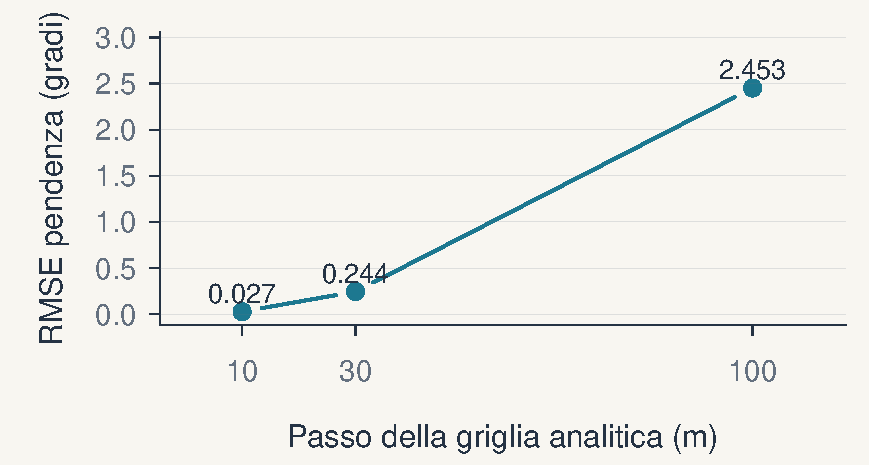
\includegraphics[width=9.85cm,height=4.55cm,keepaspectratio]{Risultati/Figure/11_sensibilita_pendenza.pdf}
\vspace{1.5mm}
\PSmall{Esperimento analitico: RMSE della pendenza alle tre risoluzioni, sullo stesso dominio fisico valido di 28 ha.}
\[\frac{f(x+h)-f(x-h)}{2h}=f'(x)+O(h^2)\]

\end{minipage}\end{lrbox}
\typeout{FULLBOX:056:PilotLeftBox:\the\ht\PilotLeftBox:\the\dp\PilotLeftBox}

\begin{lrbox}{\PilotRightBox}
\begin{minipage}[t]{7.55cm}\raggedright\color{Ink}\fontsize{11.3}{14.8}\selectfont
\PBody{Un passo più piccolo riduce l’errore di discretizzazione di una superficie regolare, ma le differenze possono amplificare il rumore delle quote.}
\vspace{2.5mm}
\PBody{Con un DEM già misurato, interpolare a una griglia più fine non equivale a ottenere nuove quote più precise.}
\vspace{2.5mm}
\PSmall{Il confronto fra scale deve distinguere errore del metodo, risoluzione del dato e variabilità della misura.}

\end{minipage}\end{lrbox}
\typeout{FULLBOX:056:PilotRightBox:\the\ht\PilotRightBox:\the\dp\PilotRightBox}

\begin{tikzpicture}[remember picture,overlay]
\PilotChrome{La precisione dipende da passo e regolarità}{V · MORFOMETRIA}{56}{La scelta del passo è legata sia alla geometria sia alla qualità dell’informazione disponibile.}
\node[anchor=north west,inner sep=0] at([xshift=.96cm,yshift=-2.13cm]current page.north west){\usebox{\PilotLeftBox}};
\node[anchor=north west,inner sep=0] at([xshift=11.52cm,yshift=-2.13cm]current page.north west){\usebox{\PilotRightBox}};
\end{tikzpicture}\end{frame}

\begin{frame}[plain]\hypertarget{slide57}{}
\bookmark[level=1,page=57]{Il gradiente conserva segno e direzione}
\begin{lrbox}{\TitleBox}
\begin{minipage}[t]{17.7cm}\raggedright\color{Ink}\fontsize{11.3}{14.8}\selectfont
\color{Navy}\bfseries\fontsize{20.6}{24.5}\selectfont Il gradiente conserva segno e direzione
\end{minipage}\end{lrbox}
\typeout{FULLBOX:057:TitleBox:\the\ht\TitleBox:\the\dp\TitleBox}

\begin{lrbox}{\RecallBox}
\begin{minipage}[t]{14.3cm}\raggedright\color{Ink}\fontsize{11.3}{14.8}\selectfont
\fontsize{10.3}{13.8}\selectfont Le due componenti devono essere lette insieme prima di ricavare pendenza ed esposizione.
\end{minipage}\end{lrbox}
\typeout{FULLBOX:057:RecallBox:\the\ht\RecallBox:\the\dp\RecallBox}

\begin{lrbox}{\FullWideBox}
\begin{minipage}[t]{18.1cm}\raggedright\color{Ink}\fontsize{11.3}{14.8}\selectfont
\centering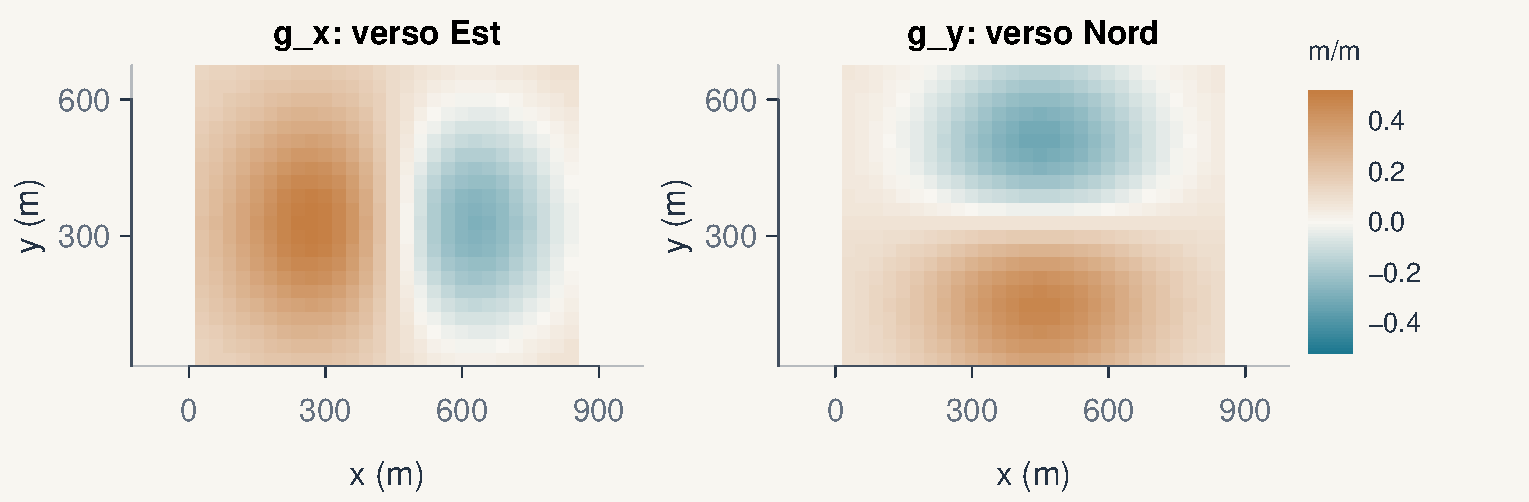
\includegraphics[width=18.05cm,height=5.8cm,keepaspectratio]{Risultati/Figure/17_gradienti_xy.pdf}
\end{minipage}\end{lrbox}
\typeout{FULLBOX:057:FullWideBox:\the\ht\FullWideBox:\the\dp\FullWideBox}

\begin{lrbox}{\PilotRightBox}
\begin{minipage}[t]{18.1cm}\raggedright\color{Ink}\fontsize{11.3}{14.8}\selectfont
\PBody{Componenti Est e Nord delle differenze centrate sul raster originale da 30 m. La scala e il segno descrivono la salita lungo ciascun asse; gli assi delle carte mantengono la convenzione locale. I margini esclusi dal calcolo non rappresentano terreno piano.}
\end{minipage}\end{lrbox}
\typeout{FULLBOX:057:PilotRightBox:\the\ht\PilotRightBox:\the\dp\PilotRightBox}

\begin{tikzpicture}[remember picture,overlay]
\PilotChrome{Il gradiente conserva segno e direzione}{V · MORFOMETRIA}{57}{Le due componenti devono essere lette insieme prima di ricavare pendenza ed esposizione.}
\node[anchor=north west,inner sep=0] at([xshift=.96cm,yshift=-2.13cm]current page.north west){\usebox{\FullWideBox}};
\node[anchor=north west,inner sep=0] at([xshift=.96cm,yshift=-8.25cm]current page.north west){\usebox{\PilotRightBox}};
\node[anchor=north east,inner sep=0] at([xshift=17.65cm,yshift=-12.06cm]current page.north west){\color{Classical}\fontsize{7.7}{9.2}\selectfont\href{../../03_Notebook_svolti/M12_Tessera/M12_N10.html}{M12\_N10 · notebook svolto}};
\end{tikzpicture}\end{frame}

\begin{frame}[plain]\hypertarget{slide58}{}
\bookmark[level=1,page=58]{La pendenza è la norma del gradiente trasformata}
\begin{lrbox}{\TitleBox}
\begin{minipage}[t]{17.7cm}\raggedright\color{Ink}\fontsize{11.3}{14.8}\selectfont
\color{Navy}\bfseries\fontsize{20.6}{24.5}\selectfont La pendenza è la norma del gradiente trasformata
\end{minipage}\end{lrbox}
\typeout{FULLBOX:058:TitleBox:\the\ht\TitleBox:\the\dp\TitleBox}

\begin{lrbox}{\RecallBox}
\begin{minipage}[t]{14.3cm}\raggedright\color{Ink}\fontsize{11.3}{14.8}\selectfont
\fontsize{10.3}{13.8}\selectfont La pendenza sintetizza l’intensità dell’inclinazione, mentre l’esposizione ne descrive la direzione.
\end{minipage}\end{lrbox}
\typeout{FULLBOX:058:RecallBox:\the\ht\RecallBox:\the\dp\RecallBox}

\begin{lrbox}{\PilotLeftBox}
\begin{minipage}[t]{10.05cm}\raggedright\color{Ink}\fontsize{11.3}{14.8}\selectfont
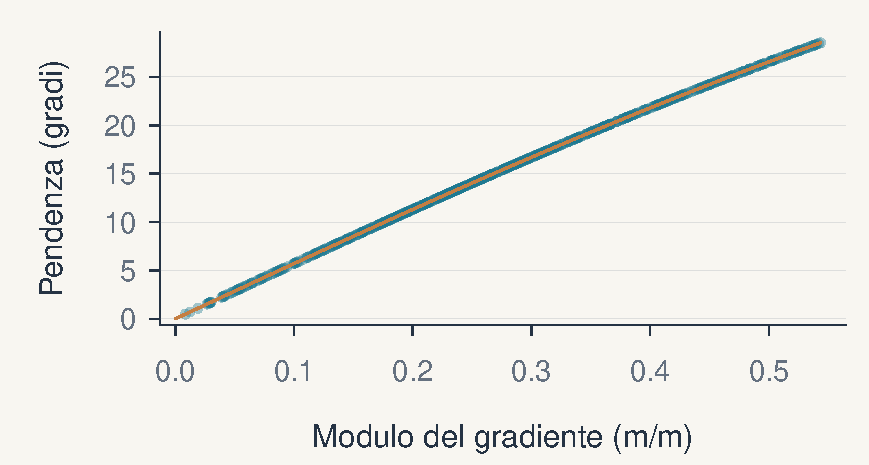
\includegraphics[width=9.85cm,height=5.25cm,keepaspectratio]{Risultati/Figure/18_gradiente_pendenza.pdf}
\vspace{1.5mm}
\PSmall{Il rapporto di massima salita $g$ e l’angolo $\alpha$ sono collegati dall’arcotangente.}
\[g=\sqrt{g_x^2+g_y^2},\qquad \alpha=\arctan g\]

\end{minipage}\end{lrbox}
\typeout{FULLBOX:058:PilotLeftBox:\the\ht\PilotLeftBox:\the\dp\PilotLeftBox}

\begin{lrbox}{\PilotRightBox}
\begin{minipage}[t]{7.55cm}\raggedright\color{Ink}\fontsize{11.3}{14.8}\selectfont
\PBody{Il gradiente indica la direzione della massima salita locale. La sua norma è il rapporto fra incremento verticale e distanza orizzontale.}
\vspace{2.5mm}
\PInfo{L’angolo perde l’informazione sulla direzione. Due versanti opposti possono avere la stessa pendenza.}
\PCode{R · due rappresentazioni}{058_esempio.R}
\end{minipage}\end{lrbox}
\typeout{FULLBOX:058:PilotRightBox:\the\ht\PilotRightBox:\the\dp\PilotRightBox}

\begin{tikzpicture}[remember picture,overlay]
\PilotChrome{La pendenza è la norma del gradiente trasformata}{V · MORFOMETRIA}{58}{La pendenza sintetizza l’intensità dell’inclinazione, mentre l’esposizione ne descrive la direzione.}
\node[anchor=north west,inner sep=0] at([xshift=.96cm,yshift=-2.13cm]current page.north west){\usebox{\PilotLeftBox}};
\node[anchor=north west,inner sep=0] at([xshift=11.52cm,yshift=-2.13cm]current page.north west){\usebox{\PilotRightBox}};
\node[anchor=north east,inner sep=0] at([xshift=17.65cm,yshift=-12.06cm]current page.north west){\color{Classical}\fontsize{7.7}{9.2}\selectfont\href{../../03_Notebook_svolti/M12_Tessera/M12_N10.html}{M12\_N10 · notebook svolto}};
\end{tikzpicture}\end{frame}

\begin{frame}[plain]\hypertarget{slide59}{}
\bookmark[level=1,page=59]{Gradi e percentuale non sono una scala lineare}
\begin{lrbox}{\TitleBox}
\begin{minipage}[t]{17.7cm}\raggedright\color{Ink}\fontsize{11.3}{14.8}\selectfont
\color{Navy}\bfseries\fontsize{20.6}{24.5}\selectfont Gradi e percentuale non sono una scala lineare
\end{minipage}\end{lrbox}
\typeout{FULLBOX:059:TitleBox:\the\ht\TitleBox:\the\dp\TitleBox}

\begin{lrbox}{\RecallBox}
\begin{minipage}[t]{14.3cm}\raggedright\color{Ink}\fontsize{11.3}{14.8}\selectfont
\fontsize{10.3}{13.8}\selectfont Le unità delle carte di pendenza devono essere esplicite prima di ogni confronto.
\end{minipage}\end{lrbox}
\typeout{FULLBOX:059:RecallBox:\the\ht\RecallBox:\the\dp\RecallBox}

\begin{lrbox}{\PilotLeftBox}
\begin{minipage}[t]{10.05cm}\raggedright\color{Ink}\fontsize{11.3}{14.8}\selectfont
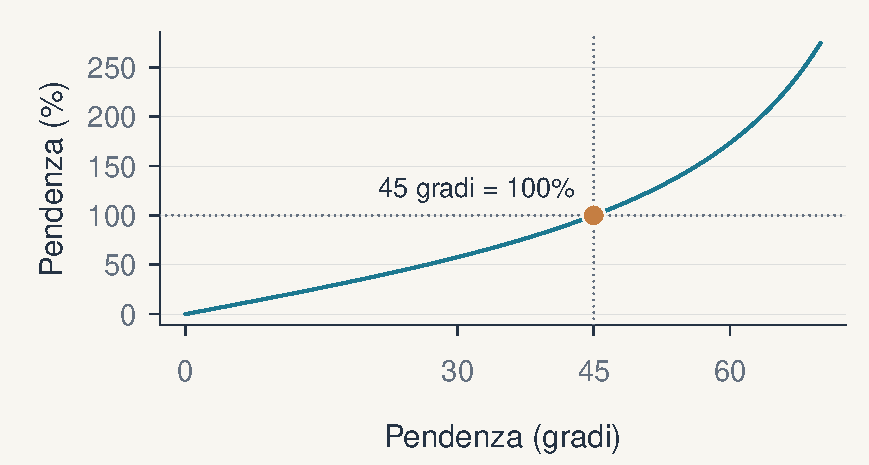
\includegraphics[width=9.85cm,height=5.25cm,keepaspectratio]{Risultati/Figure/20_gradi_percentuale.pdf}
\vspace{1.5mm}
\PSmall{45° corrispondono al 100\%; oltre 45° la percentuale supera 100 senza contraddizione.}
\[p_{\%}=100\tan\alpha\]

\end{minipage}\end{lrbox}
\typeout{FULLBOX:059:PilotLeftBox:\the\ht\PilotLeftBox:\the\dp\PilotLeftBox}

\begin{lrbox}{\PilotRightBox}
\begin{minipage}[t]{7.55cm}\raggedright\color{Ink}\fontsize{11.3}{14.8}\selectfont
\PBody{La percentuale misura il dislivello per cento unità di distanza orizzontale. L’angolo misura l’inclinazione geometrica.}
\vspace{2.5mm}
\PInfo{Una soglia espressa in gradi va convertita prima di applicarla a una carta in percentuale.}
\PCode{R · conversione non lineare}{059_esempio.R}
\end{minipage}\end{lrbox}
\typeout{FULLBOX:059:PilotRightBox:\the\ht\PilotRightBox:\the\dp\PilotRightBox}

\begin{tikzpicture}[remember picture,overlay]
\PilotChrome{Gradi e percentuale non sono una scala lineare}{V · MORFOMETRIA}{59}{Le unità delle carte di pendenza devono essere esplicite prima di ogni confronto.}
\node[anchor=north west,inner sep=0] at([xshift=.96cm,yshift=-2.13cm]current page.north west){\usebox{\PilotLeftBox}};
\node[anchor=north west,inner sep=0] at([xshift=11.52cm,yshift=-2.13cm]current page.north west){\usebox{\PilotRightBox}};
\node[anchor=north east,inner sep=0] at([xshift=17.65cm,yshift=-12.06cm]current page.north west){\color{Classical}\fontsize{7.7}{9.2}\selectfont\href{../../03_Notebook_svolti/M12_Tessera/M12_N10.html}{M12\_N10 · notebook svolto}};
\end{tikzpicture}\end{frame}

\begin{frame}[plain]\hypertarget{slide60}{}
\bookmark[level=1,page=60]{La carta delle pendenze conserva il metodo}
\begin{lrbox}{\TitleBox}
\begin{minipage}[t]{17.7cm}\raggedright\color{Ink}\fontsize{11.3}{14.8}\selectfont
\color{Navy}\bfseries\fontsize{20.6}{24.5}\selectfont La carta delle pendenze conserva il metodo
\end{minipage}\end{lrbox}
\typeout{FULLBOX:060:TitleBox:\the\ht\TitleBox:\the\dp\TitleBox}

\begin{lrbox}{\RecallBox}
\begin{minipage}[t]{14.3cm}\raggedright\color{Ink}\fontsize{11.3}{14.8}\selectfont
\fontsize{10.3}{13.8}\selectfont La legenda rende leggibile la misura; la didascalia rende ricostruibile il procedimento.
\end{minipage}\end{lrbox}
\typeout{FULLBOX:060:RecallBox:\the\ht\RecallBox:\the\dp\RecallBox}

\begin{lrbox}{\PilotLeftBox}
\begin{minipage}[t]{10.05cm}\raggedright\color{Ink}\fontsize{11.3}{14.8}\selectfont
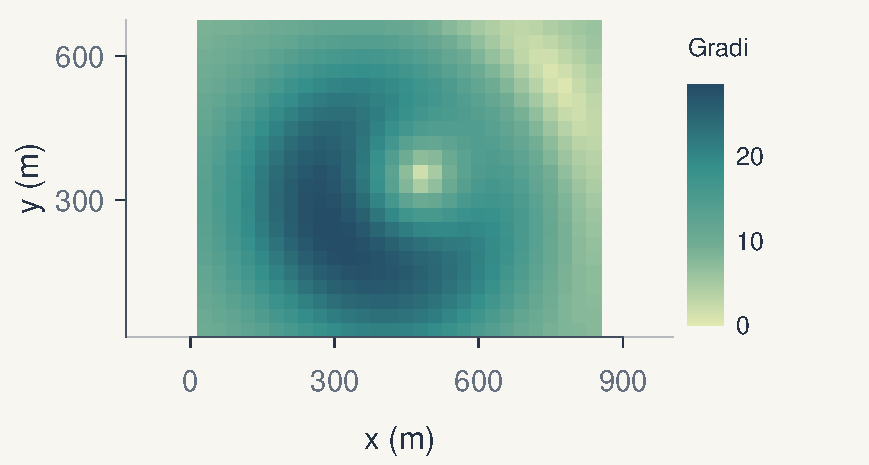
\includegraphics[width=9.85cm,height=5.25cm,keepaspectratio]{Risultati/Figure/19_pendenza_mappa.pdf}
\vspace{1.5mm}
\PSmall{Differenze centrate con quattro vicini; passo 30 m; pendenza in gradi; 22×28 celle interne.}

\end{minipage}\end{lrbox}
\typeout{FULLBOX:060:PilotLeftBox:\the\ht\PilotLeftBox:\the\dp\PilotLeftBox}

\begin{lrbox}{\PilotRightBox}
\begin{minipage}[t]{7.55cm}\raggedright\color{Ink}\fontsize{11.3}{14.8}\selectfont
\PBody{Le variazioni cromatiche rappresentano la misura derivata secondo il metodo dichiarato. Non sono direttamente la quota o la luminosità del terreno.}
\vspace{2.5mm}
\PInfo{Per confrontare due carte manteniamo uguali unità e scala cromatica, verificando anche algoritmo, risoluzione e maschere.}
\PBody{Le aree di pendenza elevata possono essere sensibili alla risoluzione e alla rappresentazione delle discontinuità.}
\vspace{2.5mm}

\end{minipage}\end{lrbox}
\typeout{FULLBOX:060:PilotRightBox:\the\ht\PilotRightBox:\the\dp\PilotRightBox}

\begin{tikzpicture}[remember picture,overlay]
\PilotChrome{La carta delle pendenze conserva il metodo}{V · MORFOMETRIA}{60}{La legenda rende leggibile la misura; la didascalia rende ricostruibile il procedimento.}
\node[anchor=north west,inner sep=0] at([xshift=.96cm,yshift=-2.13cm]current page.north west){\usebox{\PilotLeftBox}};
\node[anchor=north west,inner sep=0] at([xshift=11.52cm,yshift=-2.13cm]current page.north west){\usebox{\PilotRightBox}};
\node[anchor=north east,inner sep=0] at([xshift=17.65cm,yshift=-12.06cm]current page.north west){\color{Classical}\fontsize{7.7}{9.2}\selectfont\href{../../03_Notebook_svolti/M12_Tessera/M12_N10.html}{M12\_N10 · notebook svolto}};
\end{tikzpicture}\end{frame}

\begin{frame}[plain]\hypertarget{slide61}{}
\bookmark[level=1,page=61]{Il bordo non ha tutti i vicini richiesti}
\begin{lrbox}{\TitleBox}
\begin{minipage}[t]{17.7cm}\raggedright\color{Ink}\fontsize{11.3}{14.8}\selectfont
\color{Navy}\bfseries\fontsize{20.6}{24.5}\selectfont Il bordo non ha tutti i vicini richiesti
\end{minipage}\end{lrbox}
\typeout{FULLBOX:061:TitleBox:\the\ht\TitleBox:\the\dp\TitleBox}

\begin{lrbox}{\RecallBox}
\begin{minipage}[t]{14.3cm}\raggedright\color{Ink}\fontsize{11.3}{14.8}\selectfont
\fontsize{10.3}{13.8}\selectfont Uno zero di pendenza significa piano: non deve essere usato per codificare una derivata non calcolata.
\end{minipage}\end{lrbox}
\typeout{FULLBOX:061:RecallBox:\the\ht\RecallBox:\the\dp\RecallBox}

\begin{lrbox}{\PilotLeftBox}
\begin{minipage}[t]{10.05cm}\raggedright\color{Ink}\fontsize{11.3}{14.8}\selectfont
\[n_{\mathrm{interno}}=(24-2)(30-2)=616\]
\[n_{\mathrm{bordo}}=720-616=104\]
\PInfo{Con la convenzione adottata, le 104 celle esterne ricevono NA nella carta completa delle derivate. La loro quota originale resta disponibile.}

\end{minipage}\end{lrbox}
\typeout{FULLBOX:061:PilotLeftBox:\the\ht\PilotLeftBox:\the\dp\PilotLeftBox}

\begin{lrbox}{\PilotRightBox}
\begin{minipage}[t]{7.55cm}\raggedright\color{Ink}\fontsize{11.3}{14.8}\selectfont
\PBody{Le differenze centrate richiedono un valore da entrambi i lati. Sul bordo uno dei due manca.}
\vspace{2.5mm}
\PBody{Un altro algoritmo potrebbe usare differenze unilaterali o valori oltre il dominio. Sarebbe una scelta diversa da dichiarare e verificare.}
\vspace{2.5mm}
\PCode{R · conteggio del dominio}{061_esempio.R}
\end{minipage}\end{lrbox}
\typeout{FULLBOX:061:PilotRightBox:\the\ht\PilotRightBox:\the\dp\PilotRightBox}

\begin{tikzpicture}[remember picture,overlay]
\PilotChrome{Il bordo non ha tutti i vicini richiesti}{V · MORFOMETRIA}{61}{Uno zero di pendenza significa piano: non deve essere usato per codificare una derivata non calcolata.}
\node[anchor=north west,inner sep=0] at([xshift=.96cm,yshift=-2.13cm]current page.north west){\usebox{\PilotLeftBox}};
\node[anchor=north west,inner sep=0] at([xshift=11.52cm,yshift=-2.13cm]current page.north west){\usebox{\PilotRightBox}};
\node[anchor=north east,inner sep=0] at([xshift=17.65cm,yshift=-12.06cm]current page.north west){\color{Classical}\fontsize{7.7}{9.2}\selectfont\href{../../03_Notebook_svolti/M12_Tessera/M12_N10.html}{M12\_N10 · notebook svolto}};
\end{tikzpicture}\end{frame}

\begin{frame}[plain]\hypertarget{slide62}{}
\bookmark[level=1,page=62]{La maschera si estende alle derivate}
\begin{lrbox}{\TitleBox}
\begin{minipage}[t]{17.7cm}\raggedright\color{Ink}\fontsize{11.3}{14.8}\selectfont
\color{Navy}\bfseries\fontsize{20.6}{24.5}\selectfont La maschera si estende alle derivate
\end{minipage}\end{lrbox}
\typeout{FULLBOX:062:TitleBox:\the\ht\TitleBox:\the\dp\TitleBox}

\begin{lrbox}{\RecallBox}
\begin{minipage}[t]{14.3cm}\raggedright\color{Ink}\fontsize{11.3}{14.8}\selectfont
\fontsize{10.3}{13.8}\selectfont La maschera dell’output deriva sia dalla validità dei dati sia dalle richieste dell’algoritmo.
\end{minipage}\end{lrbox}
\typeout{FULLBOX:062:RecallBox:\the\ht\RecallBox:\the\dp\RecallBox}

\begin{lrbox}{\FullWideBox}
\begin{minipage}[t]{18.1cm}\raggedright\color{Ink}\fontsize{11.3}{14.8}\selectfont
\centering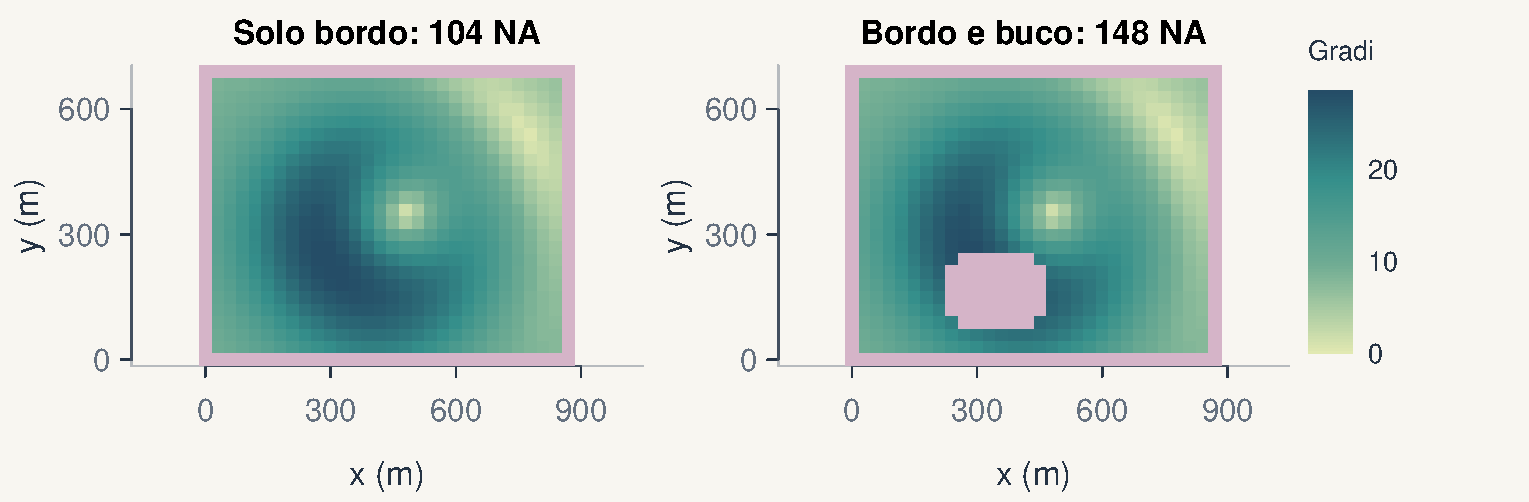
\includegraphics[width=18.05cm,height=5.8cm,keepaspectratio]{Risultati/Figure/21_bordo_maschera.pdf}
\end{minipage}\end{lrbox}
\typeout{FULLBOX:062:FullWideBox:\the\ht\FullWideBox:\the\dp\FullWideBox}

\begin{lrbox}{\PilotRightBox}
\begin{minipage}[t]{18.1cm}\raggedright\color{Ink}\fontsize{11.3}{14.8}\selectfont
\PBody{Il confronto separa il bordo esterno dal vicinato delle celle mancanti. Per le derivate del caso mascherato richiediamo centro valido e quattro vicini validi. La carta delle esclusioni documenta il motivo per cui una quota disponibile può non avere una pendenza calcolabile.}
\end{minipage}\end{lrbox}
\typeout{FULLBOX:062:PilotRightBox:\the\ht\PilotRightBox:\the\dp\PilotRightBox}

\begin{tikzpicture}[remember picture,overlay]
\PilotChrome{La maschera si estende alle derivate}{V · MORFOMETRIA}{62}{La maschera dell’output deriva sia dalla validità dei dati sia dalle richieste dell’algoritmo.}
\node[anchor=north west,inner sep=0] at([xshift=.96cm,yshift=-2.13cm]current page.north west){\usebox{\FullWideBox}};
\node[anchor=north west,inner sep=0] at([xshift=.96cm,yshift=-8.25cm]current page.north west){\usebox{\PilotRightBox}};
\end{tikzpicture}\end{frame}

\begin{frame}[plain]\hypertarget{slide63}{}
\bookmark[level=1,page=63]{L’esposizione indica la discesa}
\begin{lrbox}{\TitleBox}
\begin{minipage}[t]{17.7cm}\raggedright\color{Ink}\fontsize{11.3}{14.8}\selectfont
\color{Navy}\bfseries\fontsize{20.6}{24.5}\selectfont L’esposizione indica la discesa
\end{minipage}\end{lrbox}
\typeout{FULLBOX:063:TitleBox:\the\ht\TitleBox:\the\dp\TitleBox}

\begin{lrbox}{\RecallBox}
\begin{minipage}[t]{14.3cm}\raggedright\color{Ink}\fontsize{11.3}{14.8}\selectfont
\fontsize{10.3}{13.8}\selectfont Il segno del gradiente e la convenzione dell’azimut devono essere coerenti.
\end{minipage}\end{lrbox}
\typeout{FULLBOX:063:RecallBox:\the\ht\RecallBox:\the\dp\RecallBox}

\begin{lrbox}{\PilotLeftBox}
\begin{minipage}[t]{10.05cm}\raggedright\color{Ink}\fontsize{11.3}{14.8}\selectfont
\begin{tikzpicture}[x=1cm,y=1cm]
\path[use as bounding box](-.1,-.15) rectangle(9.7,5.65);
\draw[Rule,line width=1pt](4.7,2.7)circle(1.8);
\draw[pAxis](2.4,2.7)--(7,2.7);
\draw[pAxis](4.7,.4)--(4.7,5);
\node[pLabel]at(4.7,5.3){N: $0^\circ$};
\node[pLabel]at(7.8,2.7){E: $90^\circ$};
\node[pLabel]at(4.7,.05){S: $180^\circ$};
\node[pLabel]at(1.5,2.7){O: $270^\circ$};
\draw[-{Latex},GeoA,line width=1.6pt](4.7,2.7)--(5.95,3.95);
\draw[-{Latex},GeoB,line width=1.6pt](4.7,2.7)--(3.45,1.45);
\node[pNote,anchor=west]at(6.05,4.1){salita: $\nabla z$};
\node[pNote,anchor=east]at(3.35,1.25){discesa: $-\nabla z$};
\end{tikzpicture}
\[\theta=\operatorname{atan2}(-g_x,-g_y)\bmod2\pi\]

\end{minipage}\end{lrbox}
\typeout{FULLBOX:063:PilotLeftBox:\the\ht\PilotLeftBox:\the\dp\PilotLeftBox}

\begin{lrbox}{\PilotRightBox}
\begin{minipage}[t]{7.55cm}\raggedright\color{Ink}\fontsize{11.3}{14.8}\selectfont
\PBody{Assumiamo Est come asse $x$ e Nord come asse $y$. L’azimut cresce in senso orario dal Nord.}
\vspace{2.5mm}
\PInfo{La direzione di discesa è opposta al gradiente. La funzione atan2 distingue i quadranti e richiede l’ordine delle componenti indicato.}
\PSmall{La conversione in gradi moltiplica per $180/\pi$. I valori prossimi a 0° e 360° rappresentano direzioni vicine.}

\end{minipage}\end{lrbox}
\typeout{FULLBOX:063:PilotRightBox:\the\ht\PilotRightBox:\the\dp\PilotRightBox}

\begin{tikzpicture}[remember picture,overlay]
\PilotChrome{L’esposizione indica la discesa}{V · MORFOMETRIA}{63}{Il segno del gradiente e la convenzione dell’azimut devono essere coerenti.}
\node[anchor=north west,inner sep=0] at([xshift=.96cm,yshift=-2.13cm]current page.north west){\usebox{\PilotLeftBox}};
\node[anchor=north west,inner sep=0] at([xshift=11.52cm,yshift=-2.13cm]current page.north west){\usebox{\PilotRightBox}};
\node[anchor=north east,inner sep=0] at([xshift=17.65cm,yshift=-12.06cm]current page.north west){\color{Classical}\fontsize{7.7}{9.2}\selectfont\href{../../03_Notebook_svolti/M12_Tessera/M12_N11.html}{M12\_N11 · notebook svolto}};
\end{tikzpicture}\end{frame}

\begin{frame}[plain]\hypertarget{slide64}{}
\bookmark[level=1,page=64]{Su un piano orizzontale la direzione è indeterminata}
\begin{lrbox}{\TitleBox}
\begin{minipage}[t]{17.7cm}\raggedright\color{Ink}\fontsize{11.3}{14.8}\selectfont
\color{Navy}\bfseries\fontsize{20.6}{24.5}\selectfont Su un piano orizzontale la direzione è indeterminata
\end{minipage}\end{lrbox}
\typeout{FULLBOX:064:TitleBox:\the\ht\TitleBox:\the\dp\TitleBox}

\begin{lrbox}{\RecallBox}
\begin{minipage}[t]{14.3cm}\raggedright\color{Ink}\fontsize{11.3}{14.8}\selectfont
\fontsize{10.3}{13.8}\selectfont La mancanza di una direzione fisica deve essere distinta da un azimut numericamente valido.
\end{minipage}\end{lrbox}
\typeout{FULLBOX:064:RecallBox:\the\ht\RecallBox:\the\dp\RecallBox}

\begin{lrbox}{\PilotLeftBox}
\begin{minipage}[t]{10.05cm}\raggedright\color{Ink}\fontsize{11.3}{14.8}\selectfont
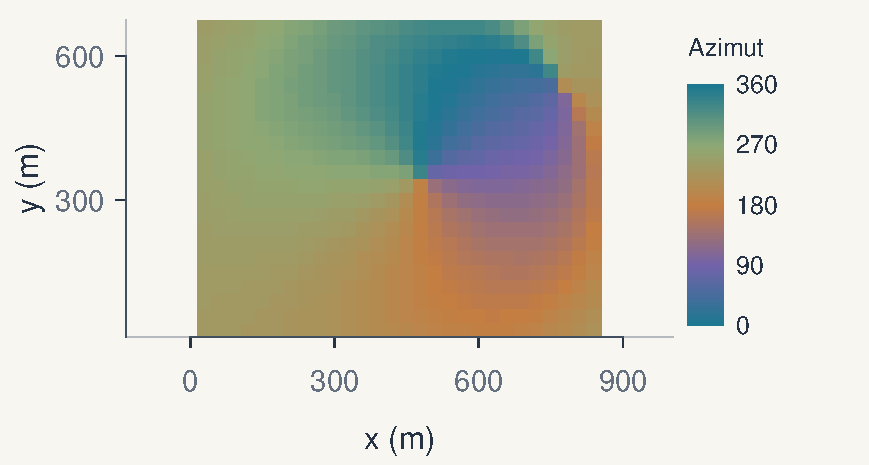
\includegraphics[width=9.85cm,height=5.25cm,keepaspectratio]{Risultati/Figure/22_aspect.pdf}
\vspace{1.5mm}
\PSmall{Esposizione in gradi, azimut orario dal Nord. La scala cromatica è circolare; il trattamento delle celle piane è esplicito.}

\end{minipage}\end{lrbox}
\typeout{FULLBOX:064:PilotLeftBox:\the\ht\PilotLeftBox:\the\dp\PilotLeftBox}

\begin{lrbox}{\PilotRightBox}
\begin{minipage}[t]{7.55cm}\raggedright\color{Ink}\fontsize{11.3}{14.8}\selectfont
\PBody{Quando il gradiente è nullo, la superficie non ha una direzione preferita di discesa. Mascheriamo quelle direzioni.}
\vspace{2.5mm}
\PInfo{Alcuni software restituiscono un valore convenzionale. Per esempio terra documenta 90° sui piani: non va interpretato come un’esposizione reale verso Est.}
\PCode{R · direzioni e celle piane}{064_esempio.R}
\end{minipage}\end{lrbox}
\typeout{FULLBOX:064:PilotRightBox:\the\ht\PilotRightBox:\the\dp\PilotRightBox}

\begin{tikzpicture}[remember picture,overlay]
\PilotChrome{Su un piano orizzontale la direzione è indeterminata}{V · MORFOMETRIA}{64}{La mancanza di una direzione fisica deve essere distinta da un azimut numericamente valido.}
\node[anchor=north west,inner sep=0] at([xshift=.96cm,yshift=-2.13cm]current page.north west){\usebox{\PilotLeftBox}};
\node[anchor=north west,inner sep=0] at([xshift=11.52cm,yshift=-2.13cm]current page.north west){\usebox{\PilotRightBox}};
\node[anchor=north east,inner sep=0] at([xshift=17.65cm,yshift=-12.06cm]current page.north west){\color{Classical}\fontsize{7.7}{9.2}\selectfont\href{../../03_Notebook_svolti/M12_Tessera/M12_N11.html}{M12\_N11 · notebook svolto}};
\end{tikzpicture}\end{frame}

\begin{frame}[plain]\hypertarget{slide65}{}
\bookmark[level=1,page=65]{Le direzioni richiedono una media circolare}
\begin{lrbox}{\TitleBox}
\begin{minipage}[t]{17.7cm}\raggedright\color{Ink}\fontsize{11.3}{14.8}\selectfont
\color{Navy}\bfseries\fontsize{20.6}{24.5}\selectfont Le direzioni richiedono una media circolare
\end{minipage}\end{lrbox}
\typeout{FULLBOX:065:TitleBox:\the\ht\TitleBox:\the\dp\TitleBox}

\begin{lrbox}{\RecallBox}
\begin{minipage}[t]{14.3cm}\raggedright\color{Ink}\fontsize{11.3}{14.8}\selectfont
\fontsize{10.3}{13.8}\selectfont Una sintesi angolare deve riconoscere la circolarità e dichiarare la concentrazione.
\end{minipage}\end{lrbox}
\typeout{FULLBOX:065:RecallBox:\the\ht\RecallBox:\the\dp\RecallBox}

\begin{lrbox}{\PilotLeftBox}
\begin{minipage}[t]{10.05cm}\raggedright\color{Ink}\fontsize{11.3}{14.8}\selectfont
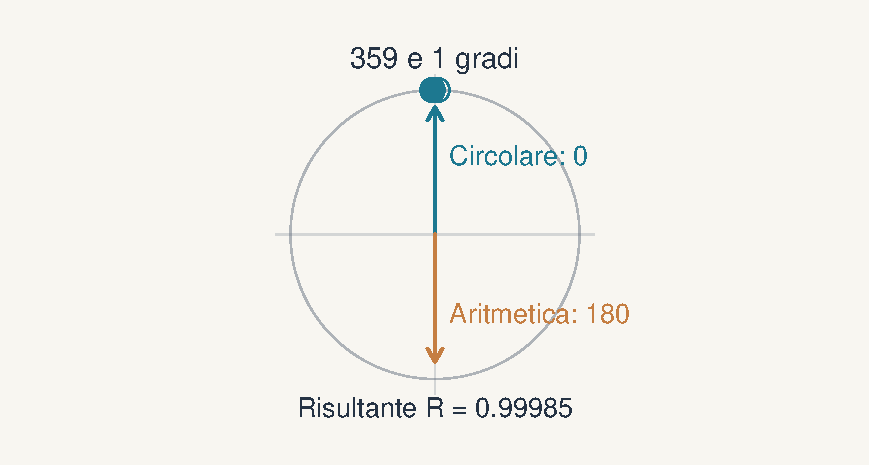
\includegraphics[width=9.85cm,height=5.25cm,keepaspectratio]{Risultati/Figure/23_media_circolare.pdf}
\vspace{1.5mm}
\PSmall{359° e 1° sono prossimi al Nord. La media aritmetica vale 180°; la media circolare riconosce la vicinanza.}
\[\overline\theta=\operatorname{atan2}(\overline S,\overline C),
 \qquad \overline R=\sqrt{\overline C^2+\overline S^2}\]

\end{minipage}\end{lrbox}
\typeout{FULLBOX:065:PilotLeftBox:\the\ht\PilotLeftBox:\the\dp\PilotLeftBox}

\begin{lrbox}{\PilotRightBox}
\begin{minipage}[t]{7.55cm}\raggedright\color{Ink}\fontsize{11.3}{14.8}\selectfont
\PBody{Calcoliamo le medie di seno e coseno. La risultante $\overline R$ descrive la concentrazione delle direzioni.}
\vspace{2.5mm}
\PInfo{Quando $\overline R$ è quasi zero, la direzione media è instabile o indeterminata. Riportiamo entrambe le quantità.}
\PCode{R · media e concentrazione}{065_esempio.R}
\end{minipage}\end{lrbox}
\typeout{FULLBOX:065:PilotRightBox:\the\ht\PilotRightBox:\the\dp\PilotRightBox}

\begin{tikzpicture}[remember picture,overlay]
\PilotChrome{Le direzioni richiedono una media circolare}{V · MORFOMETRIA}{65}{Una sintesi angolare deve riconoscere la circolarità e dichiarare la concentrazione.}
\node[anchor=north west,inner sep=0] at([xshift=.96cm,yshift=-2.13cm]current page.north west){\usebox{\PilotLeftBox}};
\node[anchor=north west,inner sep=0] at([xshift=11.52cm,yshift=-2.13cm]current page.north west){\usebox{\PilotRightBox}};
\node[anchor=north east,inner sep=0] at([xshift=17.65cm,yshift=-12.06cm]current page.north west){\color{Classical}\fontsize{7.7}{9.2}\selectfont\href{../../03_Notebook_svolti/M12_Tessera/M12_N11.html}{M12\_N11 · notebook svolto}};
\end{tikzpicture}\end{frame}

\begin{frame}[plain]\hypertarget{slide66}{}
\bookmark[level=1,page=66]{Il confronto con terra richiede lo stesso algoritmo}
\begin{lrbox}{\TitleBox}
\begin{minipage}[t]{17.7cm}\raggedright\color{Ink}\fontsize{11.3}{14.8}\selectfont
\color{Navy}\bfseries\fontsize{20.6}{24.5}\selectfont Il confronto con terra richiede lo stesso algoritmo
\end{minipage}\end{lrbox}
\typeout{FULLBOX:066:TitleBox:\the\ht\TitleBox:\the\dp\TitleBox}

\begin{lrbox}{\RecallBox}
\begin{minipage}[t]{14.3cm}\raggedright\color{Ink}\fontsize{11.3}{14.8}\selectfont
\fontsize{10.3}{13.8}\selectfont Un confronto fra software è interpretabile quando le convenzioni e il compito coincidono.
\end{minipage}\end{lrbox}
\typeout{FULLBOX:066:RecallBox:\the\ht\RecallBox:\the\dp\RecallBox}

\begin{lrbox}{\PilotLeftBox}
\begin{minipage}[t]{10.05cm}\raggedright\color{Ink}\fontsize{11.3}{14.8}\selectfont
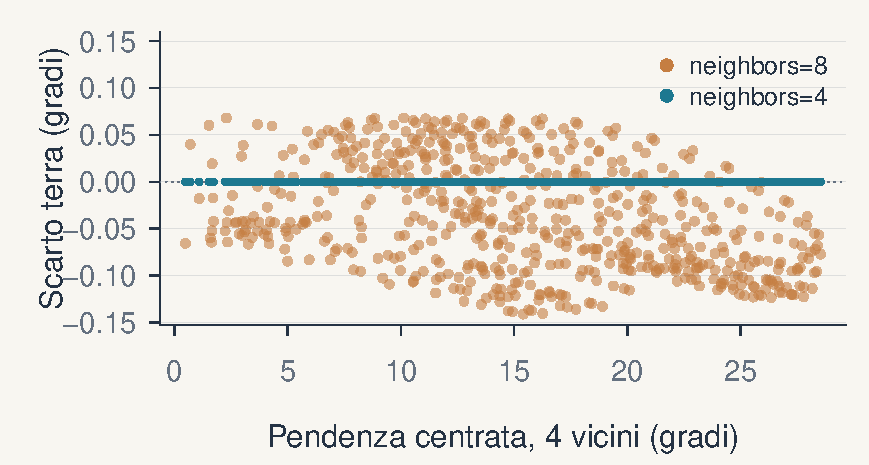
\includegraphics[width=9.85cm,height=5.25cm,keepaspectratio]{Risultati/Figure/24_confronto_terra.pdf}
\vspace{1.5mm}
\PSmall{Confronto con un algoritmo dichiarato di terra. Differenze numeriche e differenze di metodo sono valutate separatamente.}

\end{minipage}\end{lrbox}
\typeout{FULLBOX:066:PilotLeftBox:\the\ht\PilotLeftBox:\the\dp\PilotLeftBox}

\begin{lrbox}{\PilotRightBox}
\begin{minipage}[t]{7.55cm}\raggedright\color{Ink}\fontsize{11.3}{14.8}\selectfont
\PBody{terra usa otto vicini per impostazione predefinita. Per confrontare le nostre differenze centrate specifichiamo quattro vicini e le stesse unità.}
\vspace{2.5mm}
\PInfo{La gestione di bordo, mancanti e piani deve restare esplicita. Una coincidenza sul piano noto non garantisce uguaglianza per tutti i terreni.}
\PCode{R · algoritmo esplicito}{066_esempio.R}
\end{minipage}\end{lrbox}
\typeout{FULLBOX:066:PilotRightBox:\the\ht\PilotRightBox:\the\dp\PilotRightBox}

\begin{tikzpicture}[remember picture,overlay]
\PilotChrome{Il confronto con terra richiede lo stesso algoritmo}{V · MORFOMETRIA}{66}{Un confronto fra software è interpretabile quando le convenzioni e il compito coincidono.}
\node[anchor=north west,inner sep=0] at([xshift=.96cm,yshift=-2.13cm]current page.north west){\usebox{\PilotLeftBox}};
\node[anchor=north west,inner sep=0] at([xshift=11.52cm,yshift=-2.13cm]current page.north west){\usebox{\PilotRightBox}};
\node[anchor=north east,inner sep=0] at([xshift=17.65cm,yshift=-12.06cm]current page.north west){\color{Classical}\fontsize{7.7}{9.2}\selectfont\href{../../03_Notebook_svolti/M12_Tessera/M12_N10.html}{M12\_N10 · notebook svolto}};
\end{tikzpicture}\end{frame}

\begin{frame}[plain]\hypertarget{slide67}{}
\bookmark[level=0,page=67]{VI · LUCE E RILIEVO}
\bookmark[level=1,page=67]{L’ombreggiatura combina superficie e luce}
\begin{lrbox}{\TitleBox}
\begin{minipage}[t]{17.7cm}\raggedright\color{Ink}\fontsize{11.3}{14.8}\selectfont
\color{Navy}\bfseries\fontsize{20.6}{24.5}\selectfont L’ombreggiatura combina superficie e luce
\end{minipage}\end{lrbox}
\typeout{FULLBOX:067:TitleBox:\the\ht\TitleBox:\the\dp\TitleBox}

\begin{lrbox}{\RecallBox}
\begin{minipage}[t]{14.3cm}\raggedright\color{Ink}\fontsize{11.3}{14.8}\selectfont
\fontsize{10.3}{13.8}\selectfont La luce è un parametro della rappresentazione che deve accompagnare l’immagine.
\end{minipage}\end{lrbox}
\typeout{FULLBOX:067:RecallBox:\the\ht\RecallBox:\the\dp\RecallBox}

\begin{lrbox}{\PilotLeftBox}
\begin{minipage}[t]{10.05cm}\raggedright\color{Ink}\fontsize{11.3}{14.8}\selectfont
\[L=\max(0,\mathbf n\cdot\boldsymbol\ell),
       \qquad \|\mathbf n\|=\|\boldsymbol\ell\|=1\]
\begin{tikzpicture}[x=1cm,y=1cm]
\path[use as bounding box](-.1,-.15) rectangle(9.7,4.3);
\node[pFlow,text width=3.7cm,fill=GeoA!7] (a) at(2.1,3.4){Geometria del terreno};
\node[pFlow,text width=3.7cm,fill=GeoB!7] (b) at(7.3,3.4){Direzione della luce};
\node[pFlow,text width=3.7cm,fill=GeoA!7] (c) at(2.1,0.9){Normale alla superficie};
\node[pFlow,text width=3.7cm,fill=GeoC!7] (d) at(7.3,0.9){Intensità locale};
\draw[pEdge] (a) -- (c);
\draw[pEdge] (b) -- (d);
\draw[pEdge] (c) -- (d);
\end{tikzpicture}

\end{minipage}\end{lrbox}
\typeout{FULLBOX:067:PilotLeftBox:\the\ht\PilotLeftBox:\the\dp\PilotLeftBox}

\begin{lrbox}{\PilotRightBox}
\begin{minipage}[t]{7.55cm}\raggedright\color{Ink}\fontsize{11.3}{14.8}\selectfont
\PBody{Il modello lambertiano locale associa maggiore intensità alle facce orientate verso la sorgente. I contributi negativi vengono posti a zero.}
\vspace{2.5mm}
\PInfo{Il risultato è una rappresentazione dipendente dalla luce scelta. Non è una nuova misura di quota o riflettanza.}
\PBody{La normalizzazione dei vettori rende l’intensità confrontabile nell’intervallo da zero a uno.}
\vspace{2.5mm}

\end{minipage}\end{lrbox}
\typeout{FULLBOX:067:PilotRightBox:\the\ht\PilotRightBox:\the\dp\PilotRightBox}

\begin{tikzpicture}[remember picture,overlay]
\PilotChrome{L’ombreggiatura combina superficie e luce}{VI · LUCE E RILIEVO}{67}{La luce è un parametro della rappresentazione che deve accompagnare l’immagine.}
\node[anchor=north west,inner sep=0] at([xshift=.96cm,yshift=-2.13cm]current page.north west){\usebox{\PilotLeftBox}};
\node[anchor=north west,inner sep=0] at([xshift=11.52cm,yshift=-2.13cm]current page.north west){\usebox{\PilotRightBox}};
\end{tikzpicture}\end{frame}

\begin{frame}[plain]\hypertarget{slide68}{}
\bookmark[level=1,page=68]{Azimut e altezza definiscono il vettore della luce}
\begin{lrbox}{\TitleBox}
\begin{minipage}[t]{17.7cm}\raggedright\color{Ink}\fontsize{11.3}{14.8}\selectfont
\color{Navy}\bfseries\fontsize{20.6}{24.5}\selectfont Azimut e altezza definiscono il vettore della luce
\end{minipage}\end{lrbox}
\typeout{FULLBOX:068:TitleBox:\the\ht\TitleBox:\the\dp\TitleBox}

\begin{lrbox}{\RecallBox}
\begin{minipage}[t]{14.3cm}\raggedright\color{Ink}\fontsize{11.3}{14.8}\selectfont
\fontsize{10.3}{13.8}\selectfont Le convenzioni angolari devono essere dichiarate prima di tradurre la geometria in una formula.
\end{minipage}\end{lrbox}
\typeout{FULLBOX:068:RecallBox:\the\ht\RecallBox:\the\dp\RecallBox}

\begin{lrbox}{\PilotLeftBox}
\begin{minipage}[t]{10.05cm}\raggedright\color{Ink}\fontsize{11.3}{14.8}\selectfont
\[\mathbf n=\frac{(-g_x,-g_y,1)}
                        {\sqrt{1+g_x^2+g_y^2}}\]
\[\boldsymbol\ell=
       (\cos h\sin A,\;\cos h\cos A,\;\sin h)\]
\PInfo{$A$: azimut orario dal Nord. $h$: altezza sopra l’orizzonte. Quote e coordinate devono avere unità coerenti.}

\end{minipage}\end{lrbox}
\typeout{FULLBOX:068:PilotLeftBox:\the\ht\PilotLeftBox:\the\dp\PilotLeftBox}

\begin{lrbox}{\PilotRightBox}
\begin{minipage}[t]{7.55cm}\raggedright\color{Ink}\fontsize{11.3}{14.8}\selectfont
\PBody{La componente verticale della luce cresce con l’altezza. Le componenti orizzontali ne descrivono la provenienza geografica.}
\vspace{2.5mm}
\PBody{Su un terreno orizzontale $\mathbf n=(0,0,1)$ e l’intensità è $\sin h$, indipendente dall’azimut.}
\vspace{2.5mm}
\PSmall{Questo è un controllo analitico utile per riconoscere uno scambio fra altezza e angolo zenitale.}

\end{minipage}\end{lrbox}
\typeout{FULLBOX:068:PilotRightBox:\the\ht\PilotRightBox:\the\dp\PilotRightBox}

\begin{tikzpicture}[remember picture,overlay]
\PilotChrome{Azimut e altezza definiscono il vettore della luce}{VI · LUCE E RILIEVO}{68}{Le convenzioni angolari devono essere dichiarate prima di tradurre la geometria in una formula.}
\node[anchor=north west,inner sep=0] at([xshift=.96cm,yshift=-2.13cm]current page.north west){\usebox{\PilotLeftBox}};
\node[anchor=north west,inner sep=0] at([xshift=11.52cm,yshift=-2.13cm]current page.north west){\usebox{\PilotRightBox}};
\end{tikzpicture}\end{frame}

\begin{frame}[plain]\hypertarget{slide69}{}
\bookmark[level=1,page=69]{Spostare la luce cambia la carta, a quote invariate}
\begin{lrbox}{\TitleBox}
\begin{minipage}[t]{17.7cm}\raggedright\color{Ink}\fontsize{11.3}{14.8}\selectfont
\color{Navy}\bfseries\fontsize{20.6}{24.5}\selectfont Spostare la luce cambia la carta, a quote invariate
\end{minipage}\end{lrbox}
\typeout{FULLBOX:069:TitleBox:\the\ht\TitleBox:\the\dp\TitleBox}

\begin{lrbox}{\RecallBox}
\begin{minipage}[t]{14.3cm}\raggedright\color{Ink}\fontsize{11.3}{14.8}\selectfont
\fontsize{10.3}{13.8}\selectfont Confrontare più illuminazioni aiuta a distinguere la forma del terreno dall’effetto della rappresentazione.
\end{minipage}\end{lrbox}
\typeout{FULLBOX:069:RecallBox:\the\ht\RecallBox:\the\dp\RecallBox}

\begin{lrbox}{\FullWideBox}
\begin{minipage}[t]{18.1cm}\raggedright\color{Ink}\fontsize{11.3}{14.8}\selectfont
\centering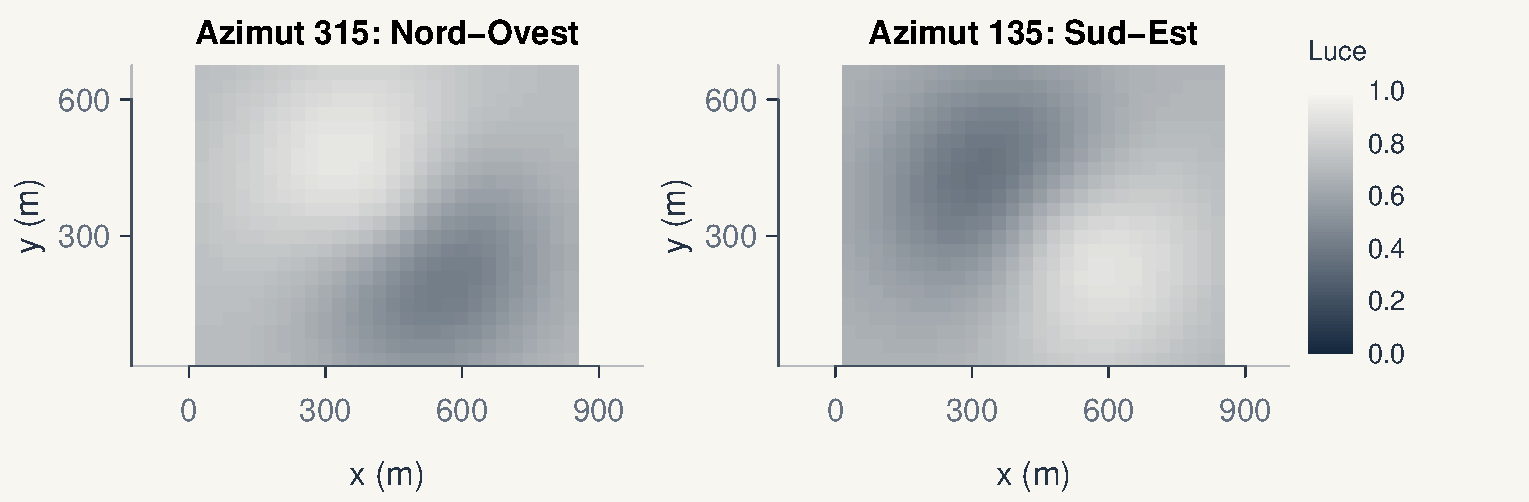
\includegraphics[width=18.05cm,height=5.8cm,keepaspectratio]{Risultati/Figure/25_hillshade_confronto.pdf}
\end{minipage}\end{lrbox}
\typeout{FULLBOX:069:FullWideBox:\the\ht\FullWideBox:\the\dp\FullWideBox}

\begin{lrbox}{\PilotRightBox}
\begin{minipage}[t]{18.1cm}\raggedright\color{Ink}\fontsize{11.3}{14.8}\selectfont
\PBody{Stesso terreno e stesse derivate, azimut 315° e 135°, altezza 45°, esagerazione verticale unitaria. La scala dell’intensità resta fissata fra 0 e 1. Le differenze derivano dalla direzione della luce; non rappresentano un cambiamento della morfologia.}
\end{minipage}\end{lrbox}
\typeout{FULLBOX:069:PilotRightBox:\the\ht\PilotRightBox:\the\dp\PilotRightBox}

\begin{tikzpicture}[remember picture,overlay]
\PilotChrome{Spostare la luce cambia la carta, a quote invariate}{VI · LUCE E RILIEVO}{69}{Confrontare più illuminazioni aiuta a distinguere la forma del terreno dall’effetto della rappresentazione.}
\node[anchor=north west,inner sep=0] at([xshift=.96cm,yshift=-2.13cm]current page.north west){\usebox{\FullWideBox}};
\node[anchor=north west,inner sep=0] at([xshift=.96cm,yshift=-8.25cm]current page.north west){\usebox{\PilotRightBox}};
\node[anchor=north east,inner sep=0] at([xshift=17.65cm,yshift=-12.06cm]current page.north west){\color{Classical}\fontsize{7.7}{9.2}\selectfont\href{../../03_Notebook_svolti/M12_Tessera/M12_N12.html}{M12\_N12 · notebook svolto}};
\end{tikzpicture}\end{frame}

\begin{frame}[plain]\hypertarget{slide70}{}
\bookmark[level=1,page=70]{Il prodotto scalare rende verificabile il calcolo}
\begin{lrbox}{\TitleBox}
\begin{minipage}[t]{17.7cm}\raggedright\color{Ink}\fontsize{11.3}{14.8}\selectfont
\color{Navy}\bfseries\fontsize{20.6}{24.5}\selectfont Il prodotto scalare rende verificabile il calcolo
\end{minipage}\end{lrbox}
\typeout{FULLBOX:070:TitleBox:\the\ht\TitleBox:\the\dp\TitleBox}

\begin{lrbox}{\RecallBox}
\begin{minipage}[t]{14.3cm}\raggedright\color{Ink}\fontsize{11.3}{14.8}\selectfont
\fontsize{10.3}{13.8}\selectfont La correttezza numerica deve conservare anche l’ordine delle celle.
\end{minipage}\end{lrbox}
\typeout{FULLBOX:070:RecallBox:\the\ht\RecallBox:\the\dp\RecallBox}

\begin{lrbox}{\PilotLeftBox}
\begin{minipage}[t]{10.05cm}\raggedright\color{Ink}\fontsize{11.3}{14.8}\selectfont
\[L=\max\left(0,
 \frac{-g_x\ell_x-g_y\ell_y+\ell_z}
      {\sqrt{1+g_x^2+g_y^2}}\right)\]
\PInfo{Il modello usa la normale orientata verso l’alto. Conserviamo righe e colonne della matrice lungo tutta l’operazione.}

\end{minipage}\end{lrbox}
\typeout{FULLBOX:070:PilotLeftBox:\the\ht\PilotLeftBox:\the\dp\PilotLeftBox}

\begin{lrbox}{\PilotRightBox}
\begin{minipage}[t]{7.55cm}\raggedright\color{Ink}\fontsize{11.3}{14.8}\selectfont
\PBody{Il codice usa radianti nelle funzioni trigonometriche e mantiene le matrici prima dello zero in pmax, preservandone gli attributi.}
\vspace{2.5mm}
\PSmall{La corrispondenza fra indice della matrice e posizione geografica viene verificata insieme ai valori.}
\PCode{R · luce da Nord-Ovest}{070_esempio.R}
\end{minipage}\end{lrbox}
\typeout{FULLBOX:070:PilotRightBox:\the\ht\PilotRightBox:\the\dp\PilotRightBox}

\begin{tikzpicture}[remember picture,overlay]
\PilotChrome{Il prodotto scalare rende verificabile il calcolo}{VI · LUCE E RILIEVO}{70}{La correttezza numerica deve conservare anche l’ordine delle celle.}
\node[anchor=north west,inner sep=0] at([xshift=.96cm,yshift=-2.13cm]current page.north west){\usebox{\PilotLeftBox}};
\node[anchor=north west,inner sep=0] at([xshift=11.52cm,yshift=-2.13cm]current page.north west){\usebox{\PilotRightBox}};
\node[anchor=north east,inner sep=0] at([xshift=17.65cm,yshift=-12.06cm]current page.north west){\color{Classical}\fontsize{7.7}{9.2}\selectfont\href{../../03_Notebook_svolti/M12_Tessera/M12_N12.html}{M12\_N12 · notebook svolto}};
\end{tikzpicture}\end{frame}

\begin{frame}[plain]\hypertarget{slide71}{}
\bookmark[level=1,page=71]{Un profilo mostra l’effetto dell’illuminazione}
\begin{lrbox}{\TitleBox}
\begin{minipage}[t]{17.7cm}\raggedright\color{Ink}\fontsize{11.3}{14.8}\selectfont
\color{Navy}\bfseries\fontsize{20.6}{24.5}\selectfont Un profilo mostra l’effetto dell’illuminazione
\end{minipage}\end{lrbox}
\typeout{FULLBOX:071:TitleBox:\the\ht\TitleBox:\the\dp\TitleBox}

\begin{lrbox}{\RecallBox}
\begin{minipage}[t]{14.3cm}\raggedright\color{Ink}\fontsize{11.3}{14.8}\selectfont
\fontsize{10.3}{13.8}\selectfont Il colore di un hillshade descrive l’illuminazione modellata, non l’altitudine.
\end{minipage}\end{lrbox}
\typeout{FULLBOX:071:RecallBox:\the\ht\RecallBox:\the\dp\RecallBox}

\begin{lrbox}{\PilotLeftBox}
\begin{minipage}[t]{10.05cm}\raggedright\color{Ink}\fontsize{11.3}{14.8}\selectfont
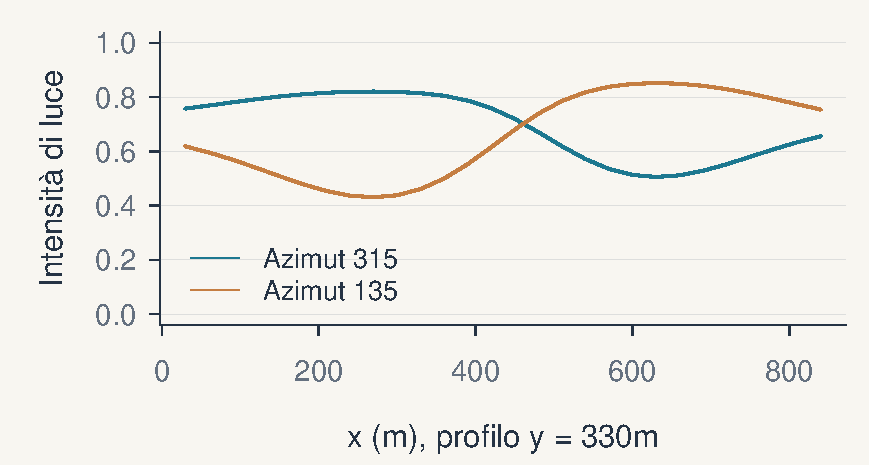
\includegraphics[width=9.85cm,height=5.25cm,keepaspectratio]{Risultati/Figure/26_illuminazione_profilo.pdf}
\vspace{1.5mm}
\PSmall{Intensità lungo un profilo del terreno al variare della luce. Quote e geometria restano fisse.}

\end{minipage}\end{lrbox}
\typeout{FULLBOX:071:PilotLeftBox:\the\ht\PilotLeftBox:\the\dp\PilotLeftBox}

\begin{lrbox}{\PilotRightBox}
\begin{minipage}[t]{7.55cm}\raggedright\color{Ink}\fontsize{11.3}{14.8}\selectfont
\PBody{Il massimo della luminosità non deve coincidere con la massima quota. Dipende dall’orientamento della superficie rispetto alla sorgente.}
\vspace{2.5mm}
\PInfo{Una scala cromatica identica permette di leggere il cambiamento senza introdurre un ulteriore effetto di riscalatura.}
\PBody{Un profilo collega le differenze visive ai valori e alle convenzioni geometriche del calcolo.}
\vspace{2.5mm}

\end{minipage}\end{lrbox}
\typeout{FULLBOX:071:PilotRightBox:\the\ht\PilotRightBox:\the\dp\PilotRightBox}

\begin{tikzpicture}[remember picture,overlay]
\PilotChrome{Un profilo mostra l’effetto dell’illuminazione}{VI · LUCE E RILIEVO}{71}{Il colore di un hillshade descrive l’illuminazione modellata, non l’altitudine.}
\node[anchor=north west,inner sep=0] at([xshift=.96cm,yshift=-2.13cm]current page.north west){\usebox{\PilotLeftBox}};
\node[anchor=north west,inner sep=0] at([xshift=11.52cm,yshift=-2.13cm]current page.north west){\usebox{\PilotRightBox}};
\node[anchor=north east,inner sep=0] at([xshift=17.65cm,yshift=-12.06cm]current page.north west){\color{Classical}\fontsize{7.7}{9.2}\selectfont\href{../../03_Notebook_svolti/M12_Tessera/M12_N12.html}{M12\_N12 · notebook svolto}};
\end{tikzpicture}\end{frame}

\begin{frame}[plain]\hypertarget{slide72}{}
\bookmark[level=1,page=72]{L’ombra locale non include tutti gli ostacoli}
\begin{lrbox}{\TitleBox}
\begin{minipage}[t]{17.7cm}\raggedright\color{Ink}\fontsize{11.3}{14.8}\selectfont
\color{Navy}\bfseries\fontsize{20.6}{24.5}\selectfont L’ombra locale non include tutti gli ostacoli
\end{minipage}\end{lrbox}
\typeout{FULLBOX:072:TitleBox:\the\ht\TitleBox:\the\dp\TitleBox}

\begin{lrbox}{\RecallBox}
\begin{minipage}[t]{14.3cm}\raggedright\color{Ink}\fontsize{11.3}{14.8}\selectfont
\fontsize{10.3}{13.8}\selectfont Un’immagine di rilievo deve essere interpretata secondo il modello con cui è stata prodotta.
\end{minipage}\end{lrbox}
\typeout{FULLBOX:072:RecallBox:\the\ht\RecallBox:\the\dp\RecallBox}

\begin{lrbox}{\PilotLeftBox}
\begin{minipage}[t]{10.05cm}\raggedright\color{Ink}\fontsize{11.3}{14.8}\selectfont
{\fontsize{10.2}{13.1}\selectfont\renewcommand{\arraystretch}{1.45}\begin{tabular}{@{}p{4.4cm}p{4.6cm}@{}}\toprule
\textbf{Nel modello locale} & \textbf{Richiede un modello ulteriore}\\\midrule
Normale della cella & Ombre proiettate da rilievi lontani\\
Direzione della sorgente & Occlusione lungo l’orizzonte\\
Intensità da prodotto scalare & Luce diffusa e riflessioni\\
Taglio dei valori negativi & Proprietà radiometriche del materiale\\
\bottomrule\end{tabular}}

\end{minipage}\end{lrbox}
\typeout{FULLBOX:072:PilotLeftBox:\the\ht\PilotLeftBox:\the\dp\PilotLeftBox}

\begin{lrbox}{\PilotRightBox}
\begin{minipage}[t]{7.55cm}\raggedright\color{Ink}\fontsize{11.3}{14.8}\selectfont
\PBody{Il calcolo locale usa l’orientamento della superficie nella cella. Non esamina automaticamente tutto il percorso dei raggi luminosi nel paesaggio.}
\vspace{2.5mm}
\PInfo{La copertina è un rendering tridimensionale con illuminazione della scena. Le figure di hillshade adottano invece il modello scientifico esplicitato qui.}
\PBody{La distinzione permette di usare correttamente entrambi i prodotti.}
\vspace{2.5mm}

\end{minipage}\end{lrbox}
\typeout{FULLBOX:072:PilotRightBox:\the\ht\PilotRightBox:\the\dp\PilotRightBox}

\begin{tikzpicture}[remember picture,overlay]
\PilotChrome{L’ombra locale non include tutti gli ostacoli}{VI · LUCE E RILIEVO}{72}{Un’immagine di rilievo deve essere interpretata secondo il modello con cui è stata prodotta.}
\node[anchor=north west,inner sep=0] at([xshift=.96cm,yshift=-2.13cm]current page.north west){\usebox{\PilotLeftBox}};
\node[anchor=north west,inner sep=0] at([xshift=11.52cm,yshift=-2.13cm]current page.north west){\usebox{\PilotRightBox}};
\end{tikzpicture}\end{frame}

\begin{frame}[plain]\hypertarget{slide73}{}
\bookmark[level=1,page=73]{L’esagerazione verticale modifica le normali}
\begin{lrbox}{\TitleBox}
\begin{minipage}[t]{17.7cm}\raggedright\color{Ink}\fontsize{11.3}{14.8}\selectfont
\color{Navy}\bfseries\fontsize{20.6}{24.5}\selectfont L’esagerazione verticale modifica le normali
\end{minipage}\end{lrbox}
\typeout{FULLBOX:073:TitleBox:\the\ht\TitleBox:\the\dp\TitleBox}

\begin{lrbox}{\RecallBox}
\begin{minipage}[t]{14.3cm}\raggedright\color{Ink}\fontsize{11.3}{14.8}\selectfont
\fontsize{10.3}{13.8}\selectfont I parametri che modificano la percezione del rilievo devono essere registrati nella didascalia.
\end{minipage}\end{lrbox}
\typeout{FULLBOX:073:RecallBox:\the\ht\RecallBox:\the\dp\RecallBox}

\begin{lrbox}{\PilotLeftBox}
\begin{minipage}[t]{10.05cm}\raggedright\color{Ink}\fontsize{11.3}{14.8}\selectfont
\[z^*=kz,\qquad \nabla z^*=k\nabla z\]
\[\alpha^*=\arctan\left(k\sqrt{g_x^2+g_y^2}\right),
       \qquad k>0\]
\PInfo{La trasformazione può accentuare le forme nella visualizzazione. Non rappresenta una nuova misura delle quote.}

\end{minipage}\end{lrbox}
\typeout{FULLBOX:073:PilotLeftBox:\the\ht\PilotLeftBox:\the\dp\PilotLeftBox}

\begin{lrbox}{\PilotRightBox}
\begin{minipage}[t]{7.55cm}\raggedright\color{Ink}\fontsize{11.3}{14.8}\selectfont
\PBody{Le pendenze apparenti e l’illuminazione cambiano perché cambia l’orientamento delle normali.}
\vspace{2.5mm}
\PBody{Nel caso principale l’esagerazione è pari a uno. Le eventuali varianti dichiarano il fattore usato e restano distinte dai dati originali.}
\vspace{2.5mm}

\end{minipage}\end{lrbox}
\typeout{FULLBOX:073:PilotRightBox:\the\ht\PilotRightBox:\the\dp\PilotRightBox}

\begin{tikzpicture}[remember picture,overlay]
\PilotChrome{L’esagerazione verticale modifica le normali}{VI · LUCE E RILIEVO}{73}{I parametri che modificano la percezione del rilievo devono essere registrati nella didascalia.}
\node[anchor=north west,inner sep=0] at([xshift=.96cm,yshift=-2.13cm]current page.north west){\usebox{\PilotLeftBox}};
\node[anchor=north west,inner sep=0] at([xshift=11.52cm,yshift=-2.13cm]current page.north west){\usebox{\PilotRightBox}};
\end{tikzpicture}\end{frame}

\begin{frame}[plain]\hypertarget{slide74}{}
\bookmark[level=1,page=74]{I controlli della luce usano casi noti}
\begin{lrbox}{\TitleBox}
\begin{minipage}[t]{17.7cm}\raggedright\color{Ink}\fontsize{11.3}{14.8}\selectfont
\color{Navy}\bfseries\fontsize{20.6}{24.5}\selectfont I controlli della luce usano casi noti
\end{minipage}\end{lrbox}
\typeout{FULLBOX:074:TitleBox:\the\ht\TitleBox:\the\dp\TitleBox}

\begin{lrbox}{\RecallBox}
\begin{minipage}[t]{14.3cm}\raggedright\color{Ink}\fontsize{11.3}{14.8}\selectfont
\fontsize{10.3}{13.8}\selectfont Le identità geometriche forniscono controlli riproducibili per la rappresentazione.
\end{minipage}\end{lrbox}
\typeout{FULLBOX:074:RecallBox:\the\ht\RecallBox:\the\dp\RecallBox}

\begin{lrbox}{\PilotLeftBox}
\begin{minipage}[t]{10.05cm}\raggedright\color{Ink}\fontsize{11.3}{14.8}\selectfont
{\fontsize{10.2}{13.1}\selectfont\renewcommand{\arraystretch}{1.45}\begin{tabular}{@{}p{4.2cm}p{4.8cm}@{}}\toprule
\textbf{Caso} & \textbf{Risultato atteso}\\\midrule
Vettori unitari & Prodotto scalare fra −1 e 1\\
Taglio locale & Intensità compresa fra 0 e 1\\
Terreno orizzontale & Intensità $\sin h$\\
Luce zenitale & Intensità $1/\sqrt{1+g^2}$\\
Cambio del solo azimut & Quote e pendenze invariate\\
\bottomrule\end{tabular}}

\end{minipage}\end{lrbox}
\typeout{FULLBOX:074:PilotLeftBox:\the\ht\PilotLeftBox:\the\dp\PilotLeftBox}

\begin{lrbox}{\PilotRightBox}
\begin{minipage}[t]{7.55cm}\raggedright\color{Ink}\fontsize{11.3}{14.8}\selectfont
\PBody{Questi controlli sono indipendenti dalla plausibilità visiva della carta. Una superficie ben ombreggiata potrebbe comunque usare una convenzione angolare errata.}
\vspace{2.5mm}
\PInfo{Verifichiamo anche la dimensione della matrice e l’associazione delle intensità con le coordinate delle celle.}
\PCode{R · limiti e piano orizzontale}{074_esempio.R}
\end{minipage}\end{lrbox}
\typeout{FULLBOX:074:PilotRightBox:\the\ht\PilotRightBox:\the\dp\PilotRightBox}

\begin{tikzpicture}[remember picture,overlay]
\PilotChrome{I controlli della luce usano casi noti}{VI · LUCE E RILIEVO}{74}{Le identità geometriche forniscono controlli riproducibili per la rappresentazione.}
\node[anchor=north west,inner sep=0] at([xshift=.96cm,yshift=-2.13cm]current page.north west){\usebox{\PilotLeftBox}};
\node[anchor=north west,inner sep=0] at([xshift=11.52cm,yshift=-2.13cm]current page.north west){\usebox{\PilotRightBox}};
\node[anchor=north east,inner sep=0] at([xshift=17.65cm,yshift=-12.06cm]current page.north west){\color{Classical}\fontsize{7.7}{9.2}\selectfont\href{../../03_Notebook_svolti/M12_Tessera/M12_N12.html}{M12\_N12 · notebook svolto}};
\end{tikzpicture}\end{frame}

\begin{frame}[plain]\hypertarget{slide75}{}
\bookmark[level=1,page=75]{Rappresentare la variabile dichiarata}
\begin{lrbox}{\TitleBox}
\begin{minipage}[t]{17.7cm}\raggedright\color{Ink}\fontsize{11.3}{14.8}\selectfont
\color{Navy}\bfseries\fontsize{20.6}{24.5}\selectfont Rappresentare la variabile dichiarata
\end{minipage}\end{lrbox}
\typeout{FULLBOX:075:TitleBox:\the\ht\TitleBox:\the\dp\TitleBox}

\begin{lrbox}{\RecallBox}
\begin{minipage}[t]{14.3cm}\raggedright\color{Ink}\fontsize{11.3}{14.8}\selectfont
\fontsize{10.3}{13.8}\selectfont La leggibilità di una carta comprende sia la legenda sia la spiegazione di come è stata costruita.
\end{minipage}\end{lrbox}
\typeout{FULLBOX:075:RecallBox:\the\ht\RecallBox:\the\dp\RecallBox}

\begin{lrbox}{\PilotLeftBox}
\begin{minipage}[t]{10.05cm}\raggedright\color{Ink}\fontsize{11.3}{14.8}\selectfont
{\fontsize{10.2}{13.1}\selectfont\renewcommand{\arraystretch}{1.45}\begin{tabular}{@{}p{3.5cm}p{5.5cm}@{}}\toprule
\textbf{Carta} & \textbf{Scala e parametri da leggere}\\\midrule
Quota & Metri e riferimento verticale\\
Pendenza & Gradi o percentuale, algoritmo\\
Esposizione & Azimut e convenzione circolare\\
Hillshade & Intensità, azimut, altezza e fattore verticale\\
Composizione grafica & Canali, trasparenze e trasformazioni\\
\bottomrule\end{tabular}}

\end{minipage}\end{lrbox}
\typeout{FULLBOX:075:PilotLeftBox:\the\ht\PilotLeftBox:\the\dp\PilotLeftBox}

\begin{lrbox}{\PilotRightBox}
\begin{minipage}[t]{7.55cm}\raggedright\color{Ink}\fontsize{11.3}{14.8}\selectfont
\PBody{Le rappresentazioni possono essere sovrapposte per facilitare l’interpretazione. Ogni componente conserva però un significato distinto.}
\vspace{2.5mm}
\PInfo{Quote, curve di livello e più illuminazioni aiutano a verificare una forma suggerita dalla percezione visiva.}
\PBody{Le didascalie devono consentire di ricostruire il prodotto anche senza vedere il codice.}
\vspace{2.5mm}

\end{minipage}\end{lrbox}
\typeout{FULLBOX:075:PilotRightBox:\the\ht\PilotRightBox:\the\dp\PilotRightBox}

\begin{tikzpicture}[remember picture,overlay]
\PilotChrome{Rappresentare la variabile dichiarata}{VI · LUCE E RILIEVO}{75}{La leggibilità di una carta comprende sia la legenda sia la spiegazione di come è stata costruita.}
\node[anchor=north west,inner sep=0] at([xshift=.96cm,yshift=-2.13cm]current page.north west){\usebox{\PilotLeftBox}};
\node[anchor=north west,inner sep=0] at([xshift=11.52cm,yshift=-2.13cm]current page.north west){\usebox{\PilotRightBox}};
\end{tikzpicture}\end{frame}

\begin{frame}[plain]\hypertarget{slide76}{}
\bookmark[level=1,page=76]{Laboratorio: verificare forma e rappresentazione}
\begin{lrbox}{\TitleBox}
\begin{minipage}[t]{17.7cm}\raggedright\color{Ink}\fontsize{11.3}{14.8}\selectfont
\color{Navy}\bfseries\fontsize{20.6}{24.5}\selectfont Laboratorio: verificare forma e rappresentazione
\end{minipage}\end{lrbox}
\typeout{FULLBOX:076:TitleBox:\the\ht\TitleBox:\the\dp\TitleBox}

\begin{lrbox}{\RecallBox}
\begin{minipage}[t]{14.3cm}\raggedright\color{Ink}\fontsize{11.3}{14.8}\selectfont
\fontsize{10.3}{13.8}\selectfont La rappresentazione del rilievo è affidabile quando parametri e verifiche rimangono accessibili.
\end{minipage}\end{lrbox}
\typeout{FULLBOX:076:RecallBox:\the\ht\RecallBox:\the\dp\RecallBox}

\begin{lrbox}{\PilotLeftBox}
\begin{minipage}[t]{10.05cm}\raggedright\color{Ink}\fontsize{11.3}{14.8}\selectfont
\PLab{https://marzione00.github.io/Lab_Geo/\#laboratorio/m12-pendenza}{Esperimento online · gradiente e pendenza}
\PLab{https://marzione00.github.io/Lab_Geo/\#laboratorio/m12-hillshade}{Esperimento online · illuminazione}
{\fontsize{10.2}{13.1}\selectfont\renewcommand{\arraystretch}{1.45}\begin{tabular}{@{}p{4.1cm}p{4.9cm}@{}}\toprule
\textbf{Attività} & \textbf{Controllo}\\\midrule
N09: piano noto & Componenti 0,12 e 0,08\\
N10: pendenza & Gradi, percentuale, bordo\\
N11: esposizione & Azimut, piani e media circolare\\
N12: hillshade & Stesso terreno, luci differenti\\
Consegna & Metodo e dominio valido delle derivate\\
\bottomrule\end{tabular}}

\end{minipage}\end{lrbox}
\typeout{FULLBOX:076:PilotLeftBox:\the\ht\PilotLeftBox:\the\dp\PilotLeftBox}

\begin{lrbox}{\PilotRightBox}
\begin{minipage}[t]{7.55cm}\raggedright\color{Ink}\fontsize{11.3}{14.8}\selectfont
\PBody{Il percorso collega formule, casi noti e carte del terreno. Ogni immagine deriva da un calcolo verificabile.}
\vspace{2.5mm}
\PInfo{La sezione successiva usa la stessa attenzione alla geometria per confrontare bande spettrali e costruire un indice.}

\end{minipage}\end{lrbox}
\typeout{FULLBOX:076:PilotRightBox:\the\ht\PilotRightBox:\the\dp\PilotRightBox}

\begin{tikzpicture}[remember picture,overlay]
\PilotChrome{Laboratorio: verificare forma e rappresentazione}{VI · LUCE E RILIEVO}{76}{La rappresentazione del rilievo è affidabile quando parametri e verifiche rimangono accessibili.}
\node[anchor=north west,inner sep=0] at([xshift=.96cm,yshift=-2.13cm]current page.north west){\usebox{\PilotLeftBox}};
\node[anchor=north west,inner sep=0] at([xshift=11.52cm,yshift=-2.13cm]current page.north west){\usebox{\PilotRightBox}};
\node[anchor=north east,inner sep=0] at([xshift=17.65cm,yshift=-12.06cm]current page.north west){\color{Classical}\fontsize{7.7}{9.2}\selectfont\href{../../03_Notebook_svolti/M12_Tessera/M12_N12.html}{M12\_N12 · notebook svolto}};
\end{tikzpicture}\end{frame}

\begin{frame}[plain]\hypertarget{slide77}{}
\bookmark[level=0,page=77]{VII · BANDE E INDICI}
\bookmark[level=1,page=77]{Le bande collegano posizione e risposta spettrale}
\begin{lrbox}{\TitleBox}
\begin{minipage}[t]{17.7cm}\raggedright\color{Ink}\fontsize{11.3}{14.8}\selectfont
\color{Navy}\bfseries\fontsize{20.6}{24.5}\selectfont Le bande collegano posizione e risposta spettrale
\end{minipage}\end{lrbox}
\typeout{FULLBOX:077:TitleBox:\the\ht\TitleBox:\the\dp\TitleBox}

\begin{lrbox}{\RecallBox}
\begin{minipage}[t]{14.3cm}\raggedright\color{Ink}\fontsize{11.3}{14.8}\selectfont
\fontsize{10.3}{13.8}\selectfont Prima del rapporto fra bande verifichiamo geometria, unità e qualità dei valori.
\end{minipage}\end{lrbox}
\typeout{FULLBOX:077:RecallBox:\the\ht\RecallBox:\the\dp\RecallBox}

\begin{lrbox}{\PilotLeftBox}
\begin{minipage}[t]{10.05cm}\raggedright\color{Ink}\fontsize{11.3}{14.8}\selectfont
\begin{tikzpicture}[x=1cm,y=1cm]
\path[use as bounding box](-.1,-.15) rectangle(9.7,5.35);
\filldraw[fill=GeoA!13,draw=GeoA](.8,1.05)--(5.8,1.05)--(8,2.45)--(3,2.45)--cycle;
\filldraw[fill=GeoB!15,draw=GeoB](.8,2.2)--(5.8,2.2)--(8,3.6)--(3,3.6)--cycle;
\filldraw[fill=GeoC!14,draw=GeoC](.8,3.35)--(5.8,3.35)--(8,4.75)--(3,4.75)--cycle;
\draw[Muted,dashed](3,2.45)--(3,4.75);
\draw[Muted,dashed](5.8,1.05)--(5.8,3.35);
\node[pNote,anchor=west]at(8.1,4.7){banda 3};
\node[pNote,anchor=west]at(8.1,3.55){banda 2};
\node[pNote,anchor=west]at(8.1,2.4){banda 1};
\node[pLabel]at(4.7,.35){stessa geometria, valori e metadati distinti};
\end{tikzpicture}

\end{minipage}\end{lrbox}
\typeout{FULLBOX:077:PilotLeftBox:\the\ht\PilotLeftBox:\the\dp\PilotLeftBox}

\begin{lrbox}{\PilotRightBox}
\begin{minipage}[t]{7.55cm}\raggedright\color{Ink}\fontsize{11.3}{14.8}\selectfont
\PBody{Una banda associa un valore a ciascuna cella per una parte dello spettro e per una specifica acquisizione. La geometria deve restare collegata ai metadati radiometrici.}
\vspace{2.5mm}
\PInfo{Il modulo usa due bande sintetiche, rosso e vicino infrarosso. Non sono immagini satellitari reali e non consentono una classificazione ecologica del territorio.}
\PBody{Il caso serve a verificare allineamento, trasformazioni numeriche e comportamento dell’indice.}
\vspace{2.5mm}

\end{minipage}\end{lrbox}
\typeout{FULLBOX:077:PilotRightBox:\the\ht\PilotRightBox:\the\dp\PilotRightBox}

\begin{tikzpicture}[remember picture,overlay]
\PilotChrome{Le bande collegano posizione e risposta spettrale}{VII · BANDE E INDICI}{77}{Prima del rapporto fra bande verifichiamo geometria, unità e qualità dei valori.}
\node[anchor=north west,inner sep=0] at([xshift=.96cm,yshift=-2.13cm]current page.north west){\usebox{\PilotLeftBox}};
\node[anchor=north west,inner sep=0] at([xshift=11.52cm,yshift=-2.13cm]current page.north west){\usebox{\PilotRightBox}};
\end{tikzpicture}\end{frame}

\begin{frame}[plain]\hypertarget{slide78}{}
\bookmark[level=1,page=78]{Due bande sintetiche sulla stessa griglia}
\begin{lrbox}{\TitleBox}
\begin{minipage}[t]{17.7cm}\raggedright\color{Ink}\fontsize{11.3}{14.8}\selectfont
\color{Navy}\bfseries\fontsize{20.6}{24.5}\selectfont Due bande sintetiche sulla stessa griglia
\end{minipage}\end{lrbox}
\typeout{FULLBOX:078:TitleBox:\the\ht\TitleBox:\the\dp\TitleBox}

\begin{lrbox}{\RecallBox}
\begin{minipage}[t]{14.3cm}\raggedright\color{Ink}\fontsize{11.3}{14.8}\selectfont
\fontsize{10.3}{13.8}\selectfont La combinazione fra bande richiede che i valori confrontati rappresentino posizioni e supporti compatibili.
\end{minipage}\end{lrbox}
\typeout{FULLBOX:078:RecallBox:\the\ht\RecallBox:\the\dp\RecallBox}

\begin{lrbox}{\FullWideBox}
\begin{minipage}[t]{18.1cm}\raggedright\color{Ink}\fontsize{11.3}{14.8}\selectfont
\centering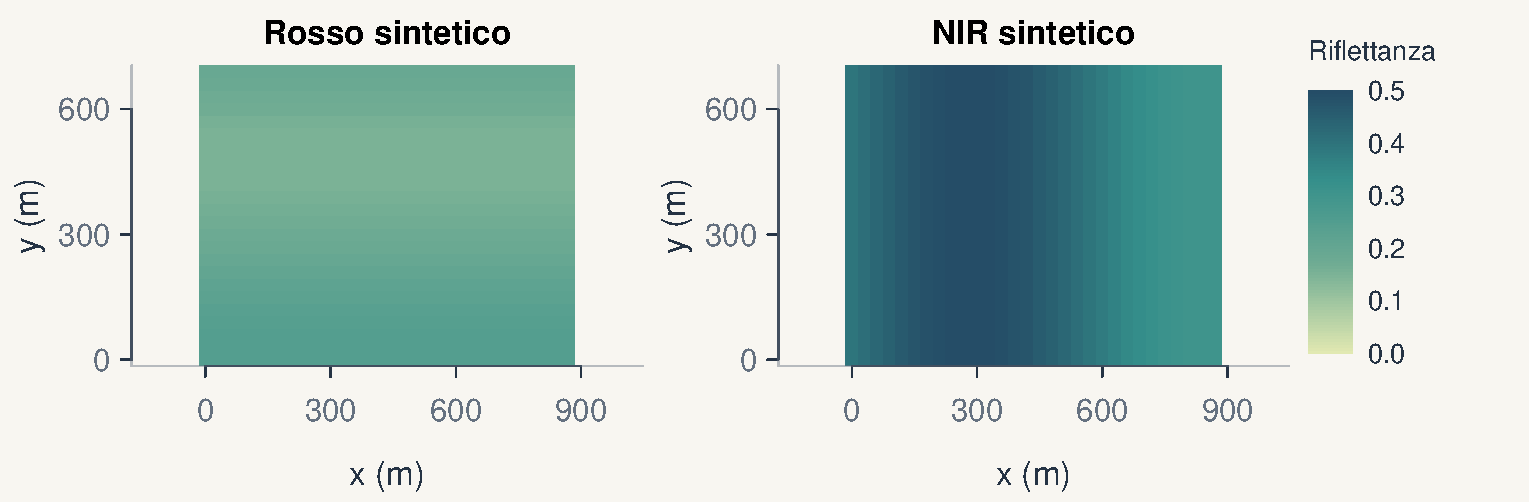
\includegraphics[width=18.05cm,height=5.8cm,keepaspectratio]{Risultati/Figure/27_bande_R_NIR.pdf}
\end{minipage}\end{lrbox}
\typeout{FULLBOX:078:FullWideBox:\the\ht\FullWideBox:\the\dp\FullWideBox}

\begin{lrbox}{\PilotRightBox}
\begin{minipage}[t]{18.1cm}\raggedright\color{Ink}\fontsize{11.3}{14.8}\selectfont
\PBody{Rosso e vicino infrarosso sono costruiti matematicamente sulla griglia locale. Le carte riportano la stessa geometria; le scale dei valori e la natura sintetica sono esplicite. L’indice verrà calcolato soltanto dopo il controllo della corrispondenza fra le celle.}
\end{minipage}\end{lrbox}
\typeout{FULLBOX:078:PilotRightBox:\the\ht\PilotRightBox:\the\dp\PilotRightBox}

\begin{tikzpicture}[remember picture,overlay]
\PilotChrome{Due bande sintetiche sulla stessa griglia}{VII · BANDE E INDICI}{78}{La combinazione fra bande richiede che i valori confrontati rappresentino posizioni e supporti compatibili.}
\node[anchor=north west,inner sep=0] at([xshift=.96cm,yshift=-2.13cm]current page.north west){\usebox{\FullWideBox}};
\node[anchor=north west,inner sep=0] at([xshift=.96cm,yshift=-8.25cm]current page.north west){\usebox{\PilotRightBox}};
\node[anchor=north east,inner sep=0] at([xshift=17.65cm,yshift=-12.06cm]current page.north west){\color{Classical}\fontsize{7.7}{9.2}\selectfont\href{../../03_Notebook_svolti/M12_Tessera/M12_N13.html}{M12\_N13 · notebook svolto}};
\end{tikzpicture}\end{frame}

\begin{frame}[plain]\hypertarget{slide79}{}
\bookmark[level=1,page=79]{Il caso sintetico rende verificabili i valori}
\begin{lrbox}{\TitleBox}
\begin{minipage}[t]{17.7cm}\raggedright\color{Ink}\fontsize{11.3}{14.8}\selectfont
\color{Navy}\bfseries\fontsize{20.6}{24.5}\selectfont Il caso sintetico rende verificabili i valori
\end{minipage}\end{lrbox}
\typeout{FULLBOX:079:TitleBox:\the\ht\TitleBox:\the\dp\TitleBox}

\begin{lrbox}{\RecallBox}
\begin{minipage}[t]{14.3cm}\raggedright\color{Ink}\fontsize{11.3}{14.8}\selectfont
\fontsize{10.3}{13.8}\selectfont La provenienza sintetica consente di conoscere le proprietà del dato prima di applicare l’indice.
\end{minipage}\end{lrbox}
\typeout{FULLBOX:079:RecallBox:\the\ht\RecallBox:\the\dp\RecallBox}

\begin{lrbox}{\PilotLeftBox}
\begin{minipage}[t]{10.05cm}\raggedright\color{Ink}\fontsize{11.3}{14.8}\selectfont
\[R(y)=0{,}20+0{,}05\cos\!\left(\frac{y}{150\ \mathrm m}\right)\]
\[N(x)=0{,}40+0{,}10\sin\!\left(\frac{x}{180\ \mathrm m}\right)\]
\PInfo{$R$ e $N$ rappresentano riflettanze sintetiche adimensionali. Gli argomenti delle funzioni trigonometriche sono adimensionali.}

\end{minipage}\end{lrbox}
\typeout{FULLBOX:079:PilotLeftBox:\the\ht\PilotLeftBox:\the\dp\PilotLeftBox}

\begin{lrbox}{\PilotRightBox}
\begin{minipage}[t]{7.55cm}\raggedright\color{Ink}\fontsize{11.3}{14.8}\selectfont
\PBody{I valori sono positivi e variano in modo controllato. L’assenza di un denominatore nullo si può verificare direttamente.}
\vspace{2.5mm}
\PSmall{Le funzioni definiscono l’esperimento didattico; non sono un modello fisico della vegetazione o di una litologia.}
\PCode{R · costruire le due bande}{079_esempio.R}
\end{minipage}\end{lrbox}
\typeout{FULLBOX:079:PilotRightBox:\the\ht\PilotRightBox:\the\dp\PilotRightBox}

\begin{tikzpicture}[remember picture,overlay]
\PilotChrome{Il caso sintetico rende verificabili i valori}{VII · BANDE E INDICI}{79}{La provenienza sintetica consente di conoscere le proprietà del dato prima di applicare l’indice.}
\node[anchor=north west,inner sep=0] at([xshift=.96cm,yshift=-2.13cm]current page.north west){\usebox{\PilotLeftBox}};
\node[anchor=north west,inner sep=0] at([xshift=11.52cm,yshift=-2.13cm]current page.north west){\usebox{\PilotRightBox}};
\node[anchor=north east,inner sep=0] at([xshift=17.65cm,yshift=-12.06cm]current page.north west){\color{Classical}\fontsize{7.7}{9.2}\selectfont\href{../../03_Notebook_svolti/M12_Tessera/M12_N13.html}{M12\_N13 · notebook svolto}};
\end{tikzpicture}\end{frame}

\begin{frame}[plain]\hypertarget{slide80}{}
\bookmark[level=1,page=80]{L’indice normalizzato misura un contrasto relativo}
\begin{lrbox}{\TitleBox}
\begin{minipage}[t]{17.7cm}\raggedright\color{Ink}\fontsize{11.3}{14.8}\selectfont
\color{Navy}\bfseries\fontsize{20.6}{24.5}\selectfont L’indice normalizzato misura un contrasto relativo
\end{minipage}\end{lrbox}
\typeout{FULLBOX:080:TitleBox:\the\ht\TitleBox:\the\dp\TitleBox}

\begin{lrbox}{\RecallBox}
\begin{minipage}[t]{14.3cm}\raggedright\color{Ink}\fontsize{11.3}{14.8}\selectfont
\fontsize{10.3}{13.8}\selectfont Un rapporto acquista significato scientifico dalle variabili che contiene e dalle condizioni del calcolo.
\end{minipage}\end{lrbox}
\typeout{FULLBOX:080:RecallBox:\the\ht\RecallBox:\the\dp\RecallBox}

\begin{lrbox}{\PilotLeftBox}
\begin{minipage}[t]{10.05cm}\raggedright\color{Ink}\fontsize{11.3}{14.8}\selectfont
\[I=\frac{N-R}{N+R}\]
\[N\ge0,\ R\ge0,\ N+R>0\quad\Longrightarrow\quad -1\le I\le1\]
\PInfo{La formula coincide con quella dell’NDVI quando $N$ e $R$ sono bande appropriate di vicino infrarosso e rosso. Qui resta un indice di bande sintetiche.}

\end{minipage}\end{lrbox}
\typeout{FULLBOX:080:PilotLeftBox:\the\ht\PilotLeftBox:\the\dp\PilotLeftBox}

\begin{lrbox}{\PilotRightBox}
\begin{minipage}[t]{7.55cm}\raggedright\color{Ink}\fontsize{11.3}{14.8}\selectfont
\PBody{Il numeratore descrive la differenza, il denominatore la normalizza rispetto alla somma. Il risultato non ha unità fisica.}
\vspace{2.5mm}
\PSmall{La normalizzazione non sostituisce le verifiche radiometriche o geometriche.}
\PCode{R · indice e condizioni}{080_esempio.R}
\end{minipage}\end{lrbox}
\typeout{FULLBOX:080:PilotRightBox:\the\ht\PilotRightBox:\the\dp\PilotRightBox}

\begin{tikzpicture}[remember picture,overlay]
\PilotChrome{L’indice normalizzato misura un contrasto relativo}{VII · BANDE E INDICI}{80}{Un rapporto acquista significato scientifico dalle variabili che contiene e dalle condizioni del calcolo.}
\node[anchor=north west,inner sep=0] at([xshift=.96cm,yshift=-2.13cm]current page.north west){\usebox{\PilotLeftBox}};
\node[anchor=north west,inner sep=0] at([xshift=11.52cm,yshift=-2.13cm]current page.north west){\usebox{\PilotRightBox}};
\node[anchor=north east,inner sep=0] at([xshift=17.65cm,yshift=-12.06cm]current page.north west){\color{Classical}\fontsize{7.7}{9.2}\selectfont\href{../../03_Notebook_svolti/M12_Tessera/M12_N13.html}{M12\_N13 · notebook svolto}};
\end{tikzpicture}\end{frame}

\begin{frame}[plain]\hypertarget{slide81}{}
\bookmark[level=1,page=81]{Lo stesso indice può derivare da valori diversi}
\begin{lrbox}{\TitleBox}
\begin{minipage}[t]{17.7cm}\raggedright\color{Ink}\fontsize{11.3}{14.8}\selectfont
\color{Navy}\bfseries\fontsize{20.6}{24.5}\selectfont Lo stesso indice può derivare da valori diversi
\end{minipage}\end{lrbox}
\typeout{FULLBOX:081:TitleBox:\the\ht\TitleBox:\the\dp\TitleBox}

\begin{lrbox}{\RecallBox}
\begin{minipage}[t]{14.3cm}\raggedright\color{Ink}\fontsize{11.3}{14.8}\selectfont
\fontsize{10.3}{13.8}\selectfont Un indice è una sintesi: il suo uso richiede di riconoscere quale informazione viene conservata.
\end{minipage}\end{lrbox}
\typeout{FULLBOX:081:RecallBox:\the\ht\RecallBox:\the\dp\RecallBox}

\begin{lrbox}{\PilotLeftBox}
\begin{minipage}[t]{10.05cm}\raggedright\color{Ink}\fontsize{11.3}{14.8}\selectfont
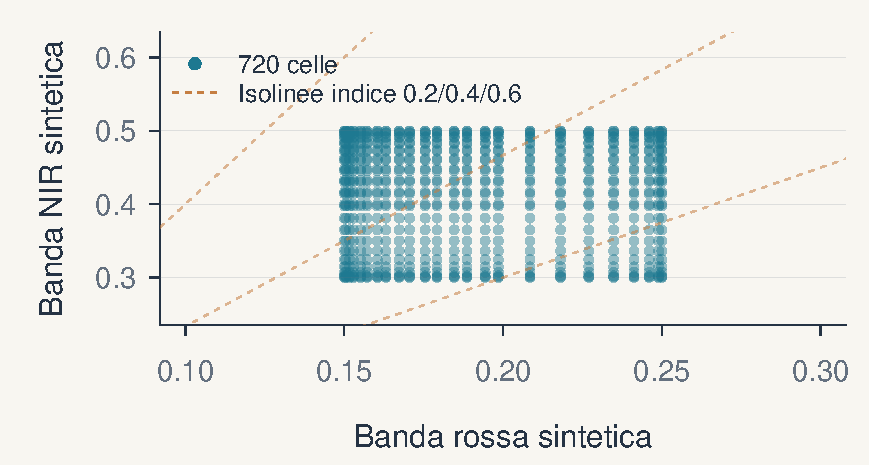
\includegraphics[width=9.85cm,height=5.25cm,keepaspectratio]{Risultati/Figure/29_spettro_indice.pdf}
\vspace{1.5mm}
\PSmall{Confronto fra valori delle bande e indice normalizzato: il rapporto sintetizza il contrasto e perde parte dell’informazione originaria.}

\end{minipage}\end{lrbox}
\typeout{FULLBOX:081:PilotLeftBox:\the\ht\PilotLeftBox:\the\dp\PilotLeftBox}

\begin{lrbox}{\PilotRightBox}
\begin{minipage}[t]{7.55cm}\raggedright\color{Ink}\fontsize{11.3}{14.8}\selectfont
\PBody{Le coppie $(R,N)=(0{,}2,0{,}4)$ e $(0{,}1,0{,}2)$ producono entrambe $I=1/3$. La somma delle bande è però diversa.}
\vspace{2.5mm}
\PInfo{Conserviamo quindi le bande e gli indicatori di qualità insieme all’indice. Un valore isolato non ricostruisce il segnale di partenza.}
\PBody{L’interpretazione dipende dal prodotto, dal supporto e dalle condizioni di acquisizione.}
\vspace{2.5mm}

\end{minipage}\end{lrbox}
\typeout{FULLBOX:081:PilotRightBox:\the\ht\PilotRightBox:\the\dp\PilotRightBox}

\begin{tikzpicture}[remember picture,overlay]
\PilotChrome{Lo stesso indice può derivare da valori diversi}{VII · BANDE E INDICI}{81}{Un indice è una sintesi: il suo uso richiede di riconoscere quale informazione viene conservata.}
\node[anchor=north west,inner sep=0] at([xshift=.96cm,yshift=-2.13cm]current page.north west){\usebox{\PilotLeftBox}};
\node[anchor=north west,inner sep=0] at([xshift=11.52cm,yshift=-2.13cm]current page.north west){\usebox{\PilotRightBox}};
\node[anchor=north east,inner sep=0] at([xshift=17.65cm,yshift=-12.06cm]current page.north west){\color{Classical}\fontsize{7.7}{9.2}\selectfont\href{../../03_Notebook_svolti/M12_Tessera/M12_N13.html}{M12\_N13 · notebook svolto}};
\end{tikzpicture}\end{frame}

\begin{frame}[plain]\hypertarget{slide82}{}
\bookmark[level=1,page=82]{Un fattore comune si cancella, un offset no}
\begin{lrbox}{\TitleBox}
\begin{minipage}[t]{17.7cm}\raggedright\color{Ink}\fontsize{11.3}{14.8}\selectfont
\color{Navy}\bfseries\fontsize{20.6}{24.5}\selectfont Un fattore comune si cancella, un offset no
\end{minipage}\end{lrbox}
\typeout{FULLBOX:082:TitleBox:\the\ht\TitleBox:\the\dp\TitleBox}

\begin{lrbox}{\RecallBox}
\begin{minipage}[t]{14.3cm}\raggedright\color{Ink}\fontsize{11.3}{14.8}\selectfont
\fontsize{10.3}{13.8}\selectfont La normalizzazione non autorizza a ignorare scale e offset radiometrici.
\end{minipage}\end{lrbox}
\typeout{FULLBOX:082:RecallBox:\the\ht\RecallBox:\the\dp\RecallBox}

\begin{lrbox}{\PilotLeftBox}
\begin{minipage}[t]{10.05cm}\raggedright\color{Ink}\fontsize{11.3}{14.8}\selectfont
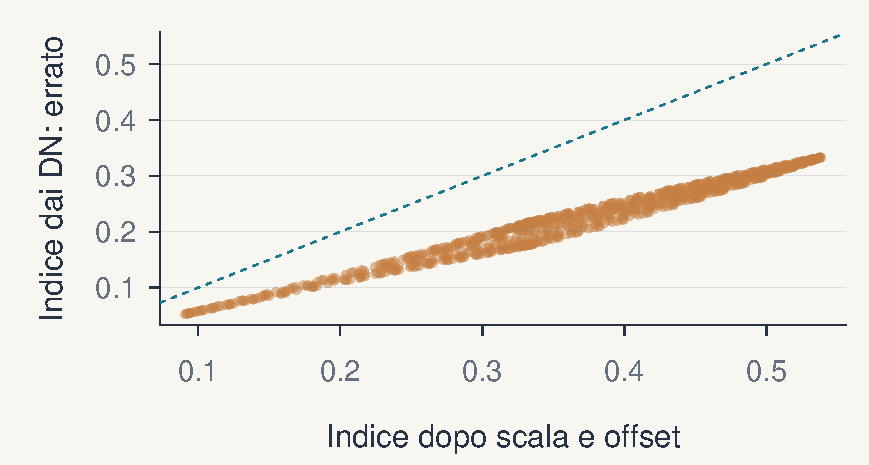
\includegraphics[width=9.85cm,height=5.25cm,keepaspectratio]{Risultati/Figure/31_scaling_offset.pdf}
\vspace{1.5mm}
\PSmall{Bande sintetiche codificate con scala e offset: indice applicato ai numeri memorizzati e indice dopo la conversione.}
\[\frac{cN-cR}{cN+cR}=\frac{N-R}{N+R},\qquad c>0\]

\end{minipage}\end{lrbox}
\typeout{FULLBOX:082:PilotLeftBox:\the\ht\PilotLeftBox:\the\dp\PilotLeftBox}

\begin{lrbox}{\PilotRightBox}
\begin{minipage}[t]{7.55cm}\raggedright\color{Ink}\fontsize{11.3}{14.8}\selectfont
\PBody{Il rapporto è invariato se entrambe le bande sono moltiplicate per lo stesso fattore positivo. Un termine additivo comune modifica invece il denominatore.}
\vspace{2.5mm}
\PInfo{Le conversioni dei valori memorizzati devono seguire i metadati del prodotto. Fattori differenti fra bande non si cancellano in generale.}
\PCode{R · invarianza verificabile}{082_esempio.R}
\end{minipage}\end{lrbox}
\typeout{FULLBOX:082:PilotRightBox:\the\ht\PilotRightBox:\the\dp\PilotRightBox}

\begin{tikzpicture}[remember picture,overlay]
\PilotChrome{Un fattore comune si cancella, un offset no}{VII · BANDE E INDICI}{82}{La normalizzazione non autorizza a ignorare scale e offset radiometrici.}
\node[anchor=north west,inner sep=0] at([xshift=.96cm,yshift=-2.13cm]current page.north west){\usebox{\PilotLeftBox}};
\node[anchor=north west,inner sep=0] at([xshift=11.52cm,yshift=-2.13cm]current page.north west){\usebox{\PilotRightBox}};
\end{tikzpicture}\end{frame}

\begin{frame}[plain]\hypertarget{slide83}{}
\bookmark[level=1,page=83]{L’allineamento delle bande precede l’algebra}
\begin{lrbox}{\TitleBox}
\begin{minipage}[t]{17.7cm}\raggedright\color{Ink}\fontsize{11.3}{14.8}\selectfont
\color{Navy}\bfseries\fontsize{20.6}{24.5}\selectfont L’allineamento delle bande precede l’algebra
\end{minipage}\end{lrbox}
\typeout{FULLBOX:083:TitleBox:\the\ht\TitleBox:\the\dp\TitleBox}

\begin{lrbox}{\RecallBox}
\begin{minipage}[t]{14.3cm}\raggedright\color{Ink}\fontsize{11.3}{14.8}\selectfont
\fontsize{10.3}{13.8}\selectfont La compatibilità numerica degli array non basta per definire un indice geograficamente coerente.
\end{minipage}\end{lrbox}
\typeout{FULLBOX:083:RecallBox:\the\ht\RecallBox:\the\dp\RecallBox}

\begin{lrbox}{\PilotLeftBox}
\begin{minipage}[t]{10.05cm}\raggedright\color{Ink}\fontsize{11.3}{14.8}\selectfont
{\fontsize{10.2}{13.1}\selectfont\renewcommand{\arraystretch}{1.45}\begin{tabular}{@{}p{4.0cm}p{5.0cm}@{}}\toprule
\textbf{Controllo} & \textbf{Motivo}\\\midrule
Stesso riferimento & Posizioni espresse nello stesso sistema\\
Stessi centri & Rapporto fra valori dello stesso luogo\\
Supporto compatibile & Confronto della stessa scala spaziale\\
Acquisizione documentata & Interpretazione delle differenze temporali\\
Qualità e maschere & Esclusione dei valori non utilizzabili\\
\bottomrule\end{tabular}}

\end{minipage}\end{lrbox}
\typeout{FULLBOX:083:PilotLeftBox:\the\ht\PilotLeftBox:\the\dp\PilotLeftBox}

\begin{lrbox}{\PilotRightBox}
\begin{minipage}[t]{7.55cm}\raggedright\color{Ink}\fontsize{11.3}{14.8}\selectfont
\PBody{Due bande con la stessa forma di matrice possono essere traslate. Il rapporto sarebbe numericamente calcolabile, ma combinerebbe luoghi diversi.}
\vspace{2.5mm}
\PInfo{Il controllo di mezzo pixel studiato in precedenza vale anche qui. Dopo un eventuale ricampionamento conserviamo metodo e griglia obiettivo.}
\PBody{Le maschere devono essere combinate sullo stesso insieme di posizioni.}
\vspace{2.5mm}

\end{minipage}\end{lrbox}
\typeout{FULLBOX:083:PilotRightBox:\the\ht\PilotRightBox:\the\dp\PilotRightBox}

\begin{tikzpicture}[remember picture,overlay]
\PilotChrome{L’allineamento delle bande precede l’algebra}{VII · BANDE E INDICI}{83}{La compatibilità numerica degli array non basta per definire un indice geograficamente coerente.}
\node[anchor=north west,inner sep=0] at([xshift=.96cm,yshift=-2.13cm]current page.north west){\usebox{\PilotLeftBox}};
\node[anchor=north west,inner sep=0] at([xshift=11.52cm,yshift=-2.13cm]current page.north west){\usebox{\PilotRightBox}};
\node[anchor=north east,inner sep=0] at([xshift=17.65cm,yshift=-12.06cm]current page.north west){\color{Classical}\fontsize{7.7}{9.2}\selectfont\href{../../03_Notebook_svolti/M12_Tessera/M12_N19.html}{M12\_N19 · notebook svolto}};
\end{tikzpicture}\end{frame}

\begin{frame}[plain]\hypertarget{slide84}{}
\bookmark[level=1,page=84]{Un denominatore piccolo amplifica le perturbazioni}
\begin{lrbox}{\TitleBox}
\begin{minipage}[t]{17.7cm}\raggedright\color{Ink}\fontsize{11.3}{14.8}\selectfont
\color{Navy}\bfseries\fontsize{20.6}{24.5}\selectfont Un denominatore piccolo amplifica le perturbazioni
\end{minipage}\end{lrbox}
\typeout{FULLBOX:084:TitleBox:\the\ht\TitleBox:\the\dp\TitleBox}

\begin{lrbox}{\RecallBox}
\begin{minipage}[t]{14.3cm}\raggedright\color{Ink}\fontsize{11.3}{14.8}\selectfont
\fontsize{10.3}{13.8}\selectfont La validità numerica e la stabilità del risultato sono proprietà da controllare separatamente.
\end{minipage}\end{lrbox}
\typeout{FULLBOX:084:RecallBox:\the\ht\RecallBox:\the\dp\RecallBox}

\begin{lrbox}{\PilotLeftBox}
\begin{minipage}[t]{10.05cm}\raggedright\color{Ink}\fontsize{11.3}{14.8}\selectfont
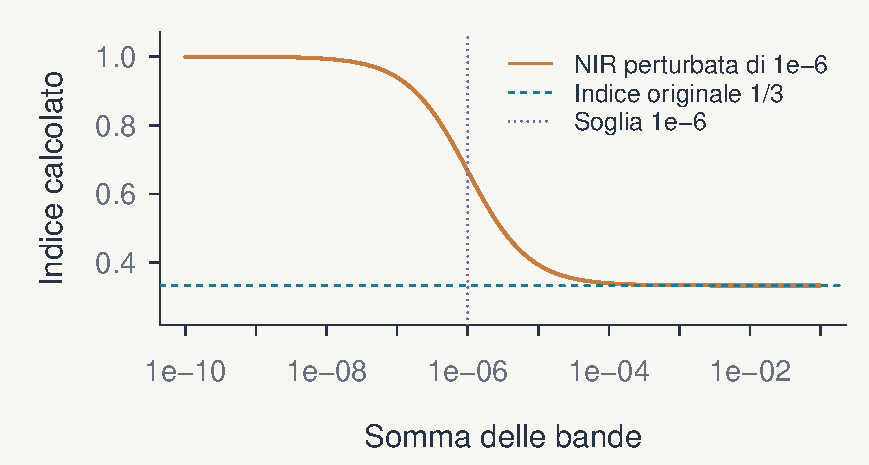
\includegraphics[width=9.85cm,height=5.25cm,keepaspectratio]{Risultati/Figure/30_denominatore.pdf}
\vspace{1.5mm}
\PSmall{Sensibilità del rapporto quando la somma delle bande si avvicina a zero. Le soglie appartengono al protocollo dichiarato.}

\end{minipage}\end{lrbox}
\typeout{FULLBOX:084:PilotLeftBox:\the\ht\PilotLeftBox:\the\dp\PilotLeftBox}

\begin{lrbox}{\PilotRightBox}
\begin{minipage}[t]{7.55cm}\raggedright\color{Ink}\fontsize{11.3}{14.8}\selectfont
\PBody{Un valore finito può essere instabile. Piccole variazioni delle bande possono produrre grandi variazioni del rapporto quando la loro somma è piccola.}
\vspace{2.5mm}
\PInfo{La soglia va scelta rispetto a precisione e rumore dei dati. Il valore $10^{-6}$ usato nell’esercizio è una convenzione didattica, non una soglia universale.}
\PBody{Il risultato deve conservare anche le celle escluse dal criterio.}
\vspace{2.5mm}

\end{minipage}\end{lrbox}
\typeout{FULLBOX:084:PilotRightBox:\the\ht\PilotRightBox:\the\dp\PilotRightBox}

\begin{tikzpicture}[remember picture,overlay]
\PilotChrome{Un denominatore piccolo amplifica le perturbazioni}{VII · BANDE E INDICI}{84}{La validità numerica e la stabilità del risultato sono proprietà da controllare separatamente.}
\node[anchor=north west,inner sep=0] at([xshift=.96cm,yshift=-2.13cm]current page.north west){\usebox{\PilotLeftBox}};
\node[anchor=north west,inner sep=0] at([xshift=11.52cm,yshift=-2.13cm]current page.north west){\usebox{\PilotRightBox}};
\node[anchor=north east,inner sep=0] at([xshift=17.65cm,yshift=-12.06cm]current page.north west){\color{Classical}\fontsize{7.7}{9.2}\selectfont\href{../../03_Notebook_svolti/M12_Tessera/M12_N14.html}{M12\_N14 · notebook svolto}};
\end{tikzpicture}\end{frame}

\begin{frame}[plain]\hypertarget{slide85}{}
\bookmark[level=1,page=85]{Le derivate descrivono la sensibilità dell’indice}
\begin{lrbox}{\TitleBox}
\begin{minipage}[t]{17.7cm}\raggedright\color{Ink}\fontsize{11.3}{14.8}\selectfont
\color{Navy}\bfseries\fontsize{20.6}{24.5}\selectfont Le derivate descrivono la sensibilità dell’indice
\end{minipage}\end{lrbox}
\typeout{FULLBOX:085:TitleBox:\the\ht\TitleBox:\the\dp\TitleBox}

\begin{lrbox}{\RecallBox}
\begin{minipage}[t]{14.3cm}\raggedright\color{Ink}\fontsize{11.3}{14.8}\selectfont
\fontsize{10.3}{13.8}\selectfont La stabilità del rapporto deve essere discussa rispetto alle perturbazioni plausibili dei dati.
\end{minipage}\end{lrbox}
\typeout{FULLBOX:085:RecallBox:\the\ht\RecallBox:\the\dp\RecallBox}

\begin{lrbox}{\PilotLeftBox}
\begin{minipage}[t]{10.05cm}\raggedright\color{Ink}\fontsize{11.3}{14.8}\selectfont
\[\frac{\partial I}{\partial N}=\frac{2R}{(N+R)^2},
       \qquad
       \frac{\partial I}{\partial R}=-\frac{2N}{(N+R)^2}\]
\[\delta I\approx
      \frac{\partial I}{\partial N}\delta N+
      \frac{\partial I}{\partial R}\delta R\]
\PInfo{Approssimazione locale al primo ordine, dove il denominatore è diverso da zero e le perturbazioni sono piccole.}

\end{minipage}\end{lrbox}
\typeout{FULLBOX:085:PilotLeftBox:\the\ht\PilotLeftBox:\the\dp\PilotLeftBox}

\begin{lrbox}{\PilotRightBox}
\begin{minipage}[t]{7.55cm}\raggedright\color{Ink}\fontsize{11.3}{14.8}\selectfont
\PBody{Le due componenti possono avere effetti opposti. La sensibilità dipende dalla somma e dai valori delle singole bande.}
\vspace{2.5mm}
\PBody{Per quantificare l’incertezza servono anche variabilità e covarianza degli errori delle bande. La formula dell’indice, da sola, non le fornisce.}
\vspace{2.5mm}

\end{minipage}\end{lrbox}
\typeout{FULLBOX:085:PilotRightBox:\the\ht\PilotRightBox:\the\dp\PilotRightBox}

\begin{tikzpicture}[remember picture,overlay]
\PilotChrome{Le derivate descrivono la sensibilità dell’indice}{VII · BANDE E INDICI}{85}{La stabilità del rapporto deve essere discussa rispetto alle perturbazioni plausibili dei dati.}
\node[anchor=north west,inner sep=0] at([xshift=.96cm,yshift=-2.13cm]current page.north west){\usebox{\PilotLeftBox}};
\node[anchor=north west,inner sep=0] at([xshift=11.52cm,yshift=-2.13cm]current page.north west){\usebox{\PilotRightBox}};
\node[anchor=north east,inner sep=0] at([xshift=17.65cm,yshift=-12.06cm]current page.north west){\color{Classical}\fontsize{7.7}{9.2}\selectfont\href{../../03_Notebook_svolti/M12_Tessera/M12_N14.html}{M12\_N14 · notebook svolto}};
\end{tikzpicture}\end{frame}

\begin{frame}[plain]\hypertarget{slide86}{}
\bookmark[level=1,page=86]{La soglia viene applicata prima della divisione}
\begin{lrbox}{\TitleBox}
\begin{minipage}[t]{17.7cm}\raggedright\color{Ink}\fontsize{11.3}{14.8}\selectfont
\color{Navy}\bfseries\fontsize{20.6}{24.5}\selectfont La soglia viene applicata prima della divisione
\end{minipage}\end{lrbox}
\typeout{FULLBOX:086:TitleBox:\the\ht\TitleBox:\the\dp\TitleBox}

\begin{lrbox}{\RecallBox}
\begin{minipage}[t]{14.3cm}\raggedright\color{Ink}\fontsize{11.3}{14.8}\selectfont
\fontsize{10.3}{13.8}\selectfont La maschera deve essere una scelta esplicita del calcolo, applicata in modo riproducibile.
\end{minipage}\end{lrbox}
\typeout{FULLBOX:086:RecallBox:\the\ht\RecallBox:\the\dp\RecallBox}

\begin{lrbox}{\PilotLeftBox}
\begin{minipage}[t]{10.05cm}\raggedright\color{Ink}\fontsize{11.3}{14.8}\selectfont
{\fontsize{10.2}{13.1}\selectfont\renewcommand{\arraystretch}{1.45}\begin{tabular}{@{}p{1.8cm}p{2.0cm}p{2.5cm}p{1.8cm}@{}}\toprule
\textbf{R} & \textbf{N} & \textbf{Somma} & \textbf{Uso}\\\midrule
0,2 & 0,4 & 0,6 & sì\\
0 & 0 & 0 & no\\
$10^{-10}$ & $2\cdot10^{-10}$ & $3\cdot10^{-10}$ & no\\
0,3 & 0,2 & 0,5 & sì\\
\bottomrule\end{tabular}}

\end{minipage}\end{lrbox}
\typeout{FULLBOX:086:PilotLeftBox:\the\ht\PilotLeftBox:\the\dp\PilotLeftBox}

\begin{lrbox}{\PilotRightBox}
\begin{minipage}[t]{7.55cm}\raggedright\color{Ink}\fontsize{11.3}{14.8}\selectfont
\PBody{Il criterio evita la divisione nelle celle escluse. Quelle celle rimangono mancanti, con una causa documentata.}
\vspace{2.5mm}
\PInfo{Abbassare la soglia per ottenere più valori finiti non garantisce un risultato più informativo.}
\PCode{R · maschera prima del rapporto}{086_esempio.R}
\end{minipage}\end{lrbox}
\typeout{FULLBOX:086:PilotRightBox:\the\ht\PilotRightBox:\the\dp\PilotRightBox}

\begin{tikzpicture}[remember picture,overlay]
\PilotChrome{La soglia viene applicata prima della divisione}{VII · BANDE E INDICI}{86}{La maschera deve essere una scelta esplicita del calcolo, applicata in modo riproducibile.}
\node[anchor=north west,inner sep=0] at([xshift=.96cm,yshift=-2.13cm]current page.north west){\usebox{\PilotLeftBox}};
\node[anchor=north west,inner sep=0] at([xshift=11.52cm,yshift=-2.13cm]current page.north west){\usebox{\PilotRightBox}};
\node[anchor=north east,inner sep=0] at([xshift=17.65cm,yshift=-12.06cm]current page.north west){\color{Classical}\fontsize{7.7}{9.2}\selectfont\href{../../03_Notebook_svolti/M12_Tessera/M12_N14.html}{M12\_N14 · notebook svolto}};
\end{tikzpicture}\end{frame}

\begin{frame}[plain]\hypertarget{slide87}{}
\bookmark[level=1,page=87]{La maschera dell’indice combina le condizioni}
\begin{lrbox}{\TitleBox}
\begin{minipage}[t]{17.7cm}\raggedright\color{Ink}\fontsize{11.3}{14.8}\selectfont
\color{Navy}\bfseries\fontsize{20.6}{24.5}\selectfont La maschera dell’indice combina le condizioni
\end{minipage}\end{lrbox}
\typeout{FULLBOX:087:TitleBox:\the\ht\TitleBox:\the\dp\TitleBox}

\begin{lrbox}{\RecallBox}
\begin{minipage}[t]{14.3cm}\raggedright\color{Ink}\fontsize{11.3}{14.8}\selectfont
\fontsize{10.3}{13.8}\selectfont Le cause di esclusione devono essere conservate prima della loro combinazione.
\end{minipage}\end{lrbox}
\typeout{FULLBOX:087:RecallBox:\the\ht\RecallBox:\the\dp\RecallBox}

\begin{lrbox}{\PilotLeftBox}
\begin{minipage}[t]{10.05cm}\raggedright\color{Ink}\fontsize{11.3}{14.8}\selectfont
\[m=m_{\mathrm{geometria}}\,
          m_{\mathrm{qualità}}\,
          m_{\mathrm{valori}}\,
          m_{\mathrm{denominatore}}\]
\PInfo{Gli indicatori valgono zero o uno. Il prodotto corrisponde alla congiunzione delle condizioni necessarie.}

\end{minipage}\end{lrbox}
\typeout{FULLBOX:087:PilotLeftBox:\the\ht\PilotLeftBox:\the\dp\PilotLeftBox}

\begin{lrbox}{\PilotRightBox}
\begin{minipage}[t]{7.55cm}\raggedright\color{Ink}\fontsize{11.3}{14.8}\selectfont
\PBody{Distinguiamo valore non finito, qualità non ammessa e somma insufficiente. La maschera finale identifica dove l’indice è utilizzabile.}
\vspace{2.5mm}
\PSmall{Nel caso sintetico principale tutte le bande sono valide; il notebook N14 costruisce i casi problematici.}
\PCode{R · dominio valido dell’indice}{087_esempio.R}
\end{minipage}\end{lrbox}
\typeout{FULLBOX:087:PilotRightBox:\the\ht\PilotRightBox:\the\dp\PilotRightBox}

\begin{tikzpicture}[remember picture,overlay]
\PilotChrome{La maschera dell’indice combina le condizioni}{VII · BANDE E INDICI}{87}{Le cause di esclusione devono essere conservate prima della loro combinazione.}
\node[anchor=north west,inner sep=0] at([xshift=.96cm,yshift=-2.13cm]current page.north west){\usebox{\PilotLeftBox}};
\node[anchor=north west,inner sep=0] at([xshift=11.52cm,yshift=-2.13cm]current page.north west){\usebox{\PilotRightBox}};
\node[anchor=north east,inner sep=0] at([xshift=17.65cm,yshift=-12.06cm]current page.north west){\color{Classical}\fontsize{7.7}{9.2}\selectfont\href{../../03_Notebook_svolti/M12_Tessera/M12_N14.html}{M12\_N14 · notebook svolto}};
\end{tikzpicture}\end{frame}

\begin{frame}[plain]\hypertarget{slide88}{}
\bookmark[level=1,page=88]{Una scala leggibile per l’indice}
\begin{lrbox}{\TitleBox}
\begin{minipage}[t]{17.7cm}\raggedright\color{Ink}\fontsize{11.3}{14.8}\selectfont
\color{Navy}\bfseries\fontsize{20.6}{24.5}\selectfont Una scala leggibile per l’indice
\end{minipage}\end{lrbox}
\typeout{FULLBOX:088:TitleBox:\the\ht\TitleBox:\the\dp\TitleBox}

\begin{lrbox}{\RecallBox}
\begin{minipage}[t]{14.3cm}\raggedright\color{Ink}\fontsize{11.3}{14.8}\selectfont
\fontsize{10.3}{13.8}\selectfont La carta deve distinguere il valore calcolato dalle interpretazioni che richiederebbero ulteriori dati.
\end{minipage}\end{lrbox}
\typeout{FULLBOX:088:RecallBox:\the\ht\RecallBox:\the\dp\RecallBox}

\begin{lrbox}{\PilotLeftBox}
\begin{minipage}[t]{10.05cm}\raggedright\color{Ink}\fontsize{11.3}{14.8}\selectfont
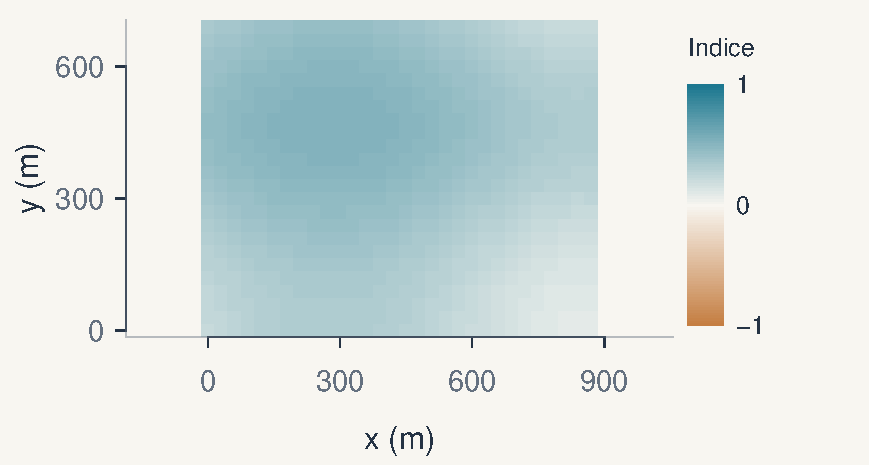
\includegraphics[width=9.85cm,height=5.25cm,keepaspectratio]{Risultati/Figure/28_indice_normalizzato.pdf}
\vspace{1.5mm}
\PSmall{Indice delle bande sintetiche sulla griglia locale. La legenda dichiara la natura adimensionale e l’intervallo rappresentato.}

\end{minipage}\end{lrbox}
\typeout{FULLBOX:088:PilotLeftBox:\the\ht\PilotLeftBox:\the\dp\PilotLeftBox}

\begin{lrbox}{\PilotRightBox}
\begin{minipage}[t]{7.55cm}\raggedright\color{Ink}\fontsize{11.3}{14.8}\selectfont
\PBody{Il colore mostra il contrasto fra le bande. Nel caso costruito non identifica automaticamente vegetazione, litologia o qualità ambientale.}
\vspace{2.5mm}
\PInfo{Per confrontare due carte usiamo scale cromatiche coerenti e riportiamo le differenze nelle maschere.}
\PBody{Le bande originali e i parametri del calcolo accompagnano l’esportazione dell’indice.}
\vspace{2.5mm}

\end{minipage}\end{lrbox}
\typeout{FULLBOX:088:PilotRightBox:\the\ht\PilotRightBox:\the\dp\PilotRightBox}

\begin{tikzpicture}[remember picture,overlay]
\PilotChrome{Una scala leggibile per l’indice}{VII · BANDE E INDICI}{88}{La carta deve distinguere il valore calcolato dalle interpretazioni che richiederebbero ulteriori dati.}
\node[anchor=north west,inner sep=0] at([xshift=.96cm,yshift=-2.13cm]current page.north west){\usebox{\PilotLeftBox}};
\node[anchor=north west,inner sep=0] at([xshift=11.52cm,yshift=-2.13cm]current page.north west){\usebox{\PilotRightBox}};
\node[anchor=north east,inner sep=0] at([xshift=17.65cm,yshift=-12.06cm]current page.north west){\color{Classical}\fontsize{7.7}{9.2}\selectfont\href{../../03_Notebook_svolti/M12_Tessera/M12_N13.html}{M12\_N13 · notebook svolto}};
\end{tikzpicture}\end{frame}

\begin{frame}[plain]\hypertarget{slide89}{}
\bookmark[level=1,page=89]{I controlli devono riconoscere dati incoerenti}
\begin{lrbox}{\TitleBox}
\begin{minipage}[t]{17.7cm}\raggedright\color{Ink}\fontsize{11.3}{14.8}\selectfont
\color{Navy}\bfseries\fontsize{20.6}{24.5}\selectfont I controlli devono riconoscere dati incoerenti
\end{minipage}\end{lrbox}
\typeout{FULLBOX:089:TitleBox:\the\ht\TitleBox:\the\dp\TitleBox}

\begin{lrbox}{\RecallBox}
\begin{minipage}[t]{14.3cm}\raggedright\color{Ink}\fontsize{11.3}{14.8}\selectfont
\fontsize{10.3}{13.8}\selectfont I controlli numerici verificano condizioni precise e non sostituiscono l’esame dei metadati.
\end{minipage}\end{lrbox}
\typeout{FULLBOX:089:RecallBox:\the\ht\RecallBox:\the\dp\RecallBox}

\begin{lrbox}{\PilotLeftBox}
\begin{minipage}[t]{10.05cm}\raggedright\color{Ink}\fontsize{11.3}{14.8}\selectfont
{\fontsize{10.2}{13.1}\selectfont\renewcommand{\arraystretch}{1.45}\begin{tabular}{@{}p{4.4cm}p{4.6cm}@{}}\toprule
\textbf{Prova} & \textbf{Aspettativa}\\\midrule
$N=R>0$ & Indice zero\\
$R=0,\ N>0$ & Indice uno\\
$N=0,\ R>0$ & Indice meno uno\\
Entrambe le bande nulle & Cella esclusa\\
Bande non negative e somma positiva & Indice fra −1 e 1\\
\bottomrule\end{tabular}}

\end{minipage}\end{lrbox}
\typeout{FULLBOX:089:PilotLeftBox:\the\ht\PilotLeftBox:\the\dp\PilotLeftBox}

\begin{lrbox}{\PilotRightBox}
\begin{minipage}[t]{7.55cm}\raggedright\color{Ink}\fontsize{11.3}{14.8}\selectfont
\PBody{Valori fuori dall’intervallo teorico richiedono di esaminare le condizioni sulle bande. Non li correggiamo automaticamente con un taglio arbitrario.}
\vspace{2.5mm}
\PInfo{Anche un indice nell’intervallo può essere sbagliato se le bande sono disallineate o hanno unità incompatibili.}
\PCode{R · casi di risultato noto}{089_esempio.R}
\end{minipage}\end{lrbox}
\typeout{FULLBOX:089:PilotRightBox:\the\ht\PilotRightBox:\the\dp\PilotRightBox}

\begin{tikzpicture}[remember picture,overlay]
\PilotChrome{I controlli devono riconoscere dati incoerenti}{VII · BANDE E INDICI}{89}{I controlli numerici verificano condizioni precise e non sostituiscono l’esame dei metadati.}
\node[anchor=north west,inner sep=0] at([xshift=.96cm,yshift=-2.13cm]current page.north west){\usebox{\PilotLeftBox}};
\node[anchor=north west,inner sep=0] at([xshift=11.52cm,yshift=-2.13cm]current page.north west){\usebox{\PilotRightBox}};
\node[anchor=north east,inner sep=0] at([xshift=17.65cm,yshift=-12.06cm]current page.north west){\color{Classical}\fontsize{7.7}{9.2}\selectfont\href{../../03_Notebook_svolti/M12_Tessera/M12_N14.html}{M12\_N14 · notebook svolto}};
\end{tikzpicture}\end{frame}

\begin{frame}[plain]\hypertarget{slide90}{}
\bookmark[level=1,page=90]{Consegna: indice e condizioni}
\begin{lrbox}{\TitleBox}
\begin{minipage}[t]{17.7cm}\raggedright\color{Ink}\fontsize{11.3}{14.8}\selectfont
\color{Navy}\bfseries\fontsize{20.6}{24.5}\selectfont Consegna: indice e condizioni
\end{minipage}\end{lrbox}
\typeout{FULLBOX:090:TitleBox:\the\ht\TitleBox:\the\dp\TitleBox}

\begin{lrbox}{\RecallBox}
\begin{minipage}[t]{14.3cm}\raggedright\color{Ink}\fontsize{11.3}{14.8}\selectfont
\fontsize{10.3}{13.8}\selectfont Un indice riproducibile include le condizioni che permettono di calcolarlo e interpretarlo.
\end{minipage}\end{lrbox}
\typeout{FULLBOX:090:RecallBox:\the\ht\RecallBox:\the\dp\RecallBox}

\begin{lrbox}{\PilotLeftBox}
\begin{minipage}[t]{10.05cm}\raggedright\color{Ink}\fontsize{11.3}{14.8}\selectfont
\PLab{https://marzione00.github.io/Lab_Geo/\#laboratorio/m12-indici}{Esperimento online · bande e indice}
{\fontsize{10.2}{13.1}\selectfont\renewcommand{\arraystretch}{1.45}\begin{tabular}{@{}p{4.3cm}p{4.7cm}@{}}\toprule
\textbf{Attività} & \textbf{Evidenza}\\\midrule
N13: bande sintetiche & Formule, geometria e valori\\
N14: denominatore & Soglia e celle escluse\\
Controllo algebrico & Casi noti e fattore comune\\
Controllo geografico & Corrispondenza delle celle\\
Consegna & Indice, maschera e provenienza\\
\bottomrule\end{tabular}}

\end{minipage}\end{lrbox}
\typeout{FULLBOX:090:PilotLeftBox:\the\ht\PilotLeftBox:\the\dp\PilotLeftBox}

\begin{lrbox}{\PilotRightBox}
\begin{minipage}[t]{7.55cm}\raggedright\color{Ink}\fontsize{11.3}{14.8}\selectfont
\PBody{La relazione deve rendere chiaro che cosa rappresenta il rapporto e quali condizioni lo rendono utilizzabile.}
\vspace{2.5mm}
\PInfo{Le sintesi territoriali successive conserveranno la maschera, il dominio e i pesi: il passaggio a una tabella non elimina la struttura spaziale.}

\end{minipage}\end{lrbox}
\typeout{FULLBOX:090:PilotRightBox:\the\ht\PilotRightBox:\the\dp\PilotRightBox}

\begin{tikzpicture}[remember picture,overlay]
\PilotChrome{Consegna: indice e condizioni}{VII · BANDE E INDICI}{90}{Un indice riproducibile include le condizioni che permettono di calcolarlo e interpretarlo.}
\node[anchor=north west,inner sep=0] at([xshift=.96cm,yshift=-2.13cm]current page.north west){\usebox{\PilotLeftBox}};
\node[anchor=north west,inner sep=0] at([xshift=11.52cm,yshift=-2.13cm]current page.north west){\usebox{\PilotRightBox}};
\node[anchor=north east,inner sep=0] at([xshift=17.65cm,yshift=-12.06cm]current page.north west){\color{Classical}\fontsize{7.7}{9.2}\selectfont\href{../../03_Notebook_svolti/M12_Tessera/M12_N14.html}{M12\_N14 · notebook svolto}};
\end{tikzpicture}\end{frame}

\begin{frame}[plain]\hypertarget{slide91}{}
\bookmark[level=0,page=91]{VIII · SINTESI TERRITORIALI}
\bookmark[level=1,page=91]{Le zone cambiano l’unità della tabella}
\begin{lrbox}{\TitleBox}
\begin{minipage}[t]{17.7cm}\raggedright\color{Ink}\fontsize{11.3}{14.8}\selectfont
\color{Navy}\bfseries\fontsize{20.6}{24.5}\selectfont Le zone cambiano l’unità della tabella
\end{minipage}\end{lrbox}
\typeout{FULLBOX:091:TitleBox:\the\ht\TitleBox:\the\dp\TitleBox}

\begin{lrbox}{\RecallBox}
\begin{minipage}[t]{14.3cm}\raggedright\color{Ink}\fontsize{11.3}{14.8}\selectfont
\fontsize{10.3}{13.8}\selectfont Passare dalle celle alle zone cambia l’unità statistica e il significato della riga.
\end{minipage}\end{lrbox}
\typeout{FULLBOX:091:RecallBox:\the\ht\RecallBox:\the\dp\RecallBox}

\begin{lrbox}{\PilotLeftBox}
\begin{minipage}[t]{10.05cm}\raggedright\color{Ink}\fontsize{11.3}{14.8}\selectfont
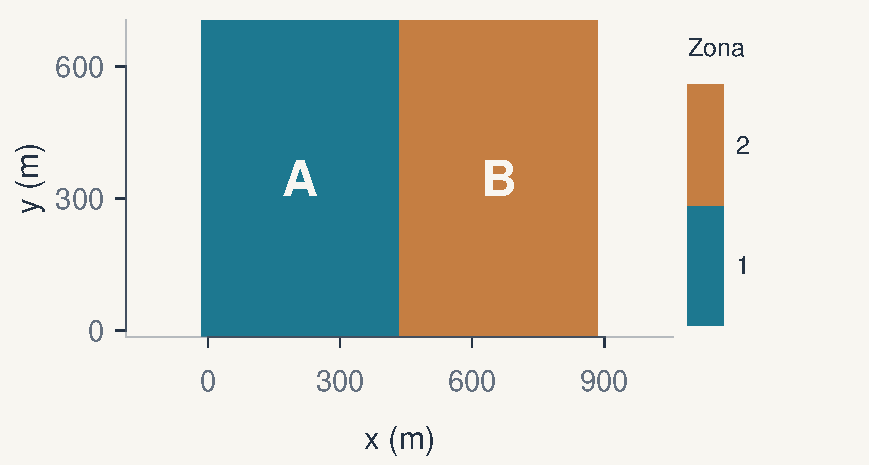
\includegraphics[width=9.85cm,height=5.25cm,keepaspectratio]{Risultati/Figure/32_zone.pdf}
\vspace{1.5mm}
\PSmall{Zone didattiche A e B sullo stesso terreno: 360 celle per zona, ciascuna di area piana 0,09 ha.}

\end{minipage}\end{lrbox}
\typeout{FULLBOX:091:PilotLeftBox:\the\ht\PilotLeftBox:\the\dp\PilotLeftBox}

\begin{lrbox}{\PilotRightBox}
\begin{minipage}[t]{7.55cm}\raggedright\color{Ink}\fontsize{11.3}{14.8}\selectfont
\PBody{Una sintesi zonale produce una riga per regione. I valori riassumono insiemi di celle definiti da una regola di appartenenza.}
\vspace{2.5mm}
\PInfo{A e B sono convenzioni del caso sintetico. Non rappresentano gruppi sperimentali assegnati casualmente né unità geologiche osservate.}
\PBody{Conserviamo numerosità, area e copertura insieme alla statistica.}
\vspace{2.5mm}

\end{minipage}\end{lrbox}
\typeout{FULLBOX:091:PilotRightBox:\the\ht\PilotRightBox:\the\dp\PilotRightBox}

\begin{tikzpicture}[remember picture,overlay]
\PilotChrome{Le zone cambiano l’unità della tabella}{VIII · SINTESI TERRITORIALI}{91}{Passare dalle celle alle zone cambia l’unità statistica e il significato della riga.}
\node[anchor=north west,inner sep=0] at([xshift=.96cm,yshift=-2.13cm]current page.north west){\usebox{\PilotLeftBox}};
\node[anchor=north west,inner sep=0] at([xshift=11.52cm,yshift=-2.13cm]current page.north west){\usebox{\PilotRightBox}};
\node[anchor=north east,inner sep=0] at([xshift=17.65cm,yshift=-12.06cm]current page.north west){\color{Classical}\fontsize{7.7}{9.2}\selectfont\href{../../03_Notebook_svolti/M12_Tessera/M12_N15.html}{M12\_N15 · notebook svolto}};
\end{tikzpicture}\end{frame}

\begin{frame}[plain]\hypertarget{slide92}{}
\bookmark[level=1,page=92]{Media e dispersione nella stessa zona}
\begin{lrbox}{\TitleBox}
\begin{minipage}[t]{17.7cm}\raggedright\color{Ink}\fontsize{11.3}{14.8}\selectfont
\color{Navy}\bfseries\fontsize{20.6}{24.5}\selectfont Media e dispersione nella stessa zona
\end{minipage}\end{lrbox}
\typeout{FULLBOX:092:TitleBox:\the\ht\TitleBox:\the\dp\TitleBox}

\begin{lrbox}{\RecallBox}
\begin{minipage}[t]{14.3cm}\raggedright\color{Ink}\fontsize{11.3}{14.8}\selectfont
\fontsize{10.3}{13.8}\selectfont Una tabella zonale deve conservare gli elementi necessari a ricostruire il bersaglio della sintesi.
\end{minipage}\end{lrbox}
\typeout{FULLBOX:092:RecallBox:\the\ht\RecallBox:\the\dp\RecallBox}

\begin{lrbox}{\PilotLeftBox}
\begin{minipage}[t]{10.05cm}\raggedright\color{Ink}\fontsize{11.3}{14.8}\selectfont
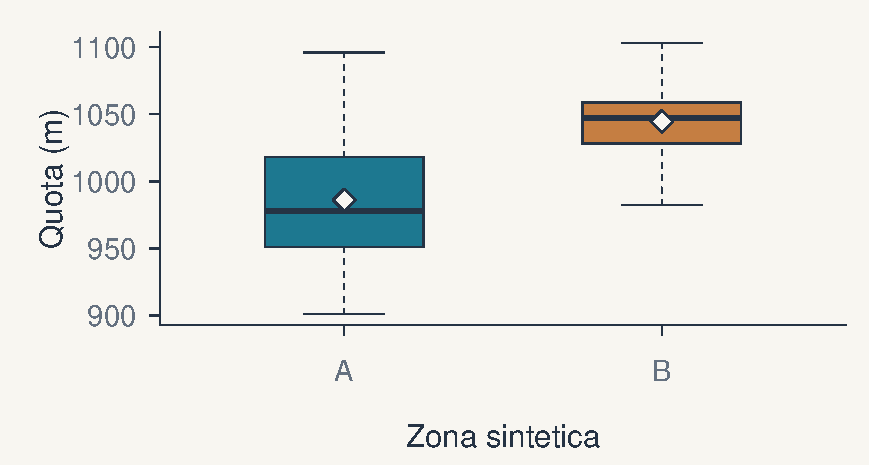
\includegraphics[width=9.85cm,height=5.25cm,keepaspectratio]{Risultati/Figure/33_sintesi_zonali.pdf}
\vspace{1.5mm}
\PSmall{Sintesi delle quote nelle due zone: livello, dispersione e numerosità devono essere letti insieme.}

\end{minipage}\end{lrbox}
\typeout{FULLBOX:092:PilotLeftBox:\the\ht\PilotLeftBox:\the\dp\PilotLeftBox}

\begin{lrbox}{\PilotRightBox}
\begin{minipage}[t]{7.55cm}\raggedright\color{Ink}\fontsize{11.3}{14.8}\selectfont
\PBody{La media descrive il livello delle quote. La dispersione descrive la variabilità interna; la copertura identifica il dominio disponibile.}
\vspace{2.5mm}
\PInfo{La differenza fra le zone riflette la loro collocazione sul terreno sintetico. Non viene interpretata come effetto causale dell’etichetta.}
\PCode{R · livello e conteggi}{092_esempio.R}
\end{minipage}\end{lrbox}
\typeout{FULLBOX:092:PilotRightBox:\the\ht\PilotRightBox:\the\dp\PilotRightBox}

\begin{tikzpicture}[remember picture,overlay]
\PilotChrome{Media e dispersione nella stessa zona}{VIII · SINTESI TERRITORIALI}{92}{Una tabella zonale deve conservare gli elementi necessari a ricostruire il bersaglio della sintesi.}
\node[anchor=north west,inner sep=0] at([xshift=.96cm,yshift=-2.13cm]current page.north west){\usebox{\PilotLeftBox}};
\node[anchor=north west,inner sep=0] at([xshift=11.52cm,yshift=-2.13cm]current page.north west){\usebox{\PilotRightBox}};
\node[anchor=north east,inner sep=0] at([xshift=17.65cm,yshift=-12.06cm]current page.north west){\color{Classical}\fontsize{7.7}{9.2}\selectfont\href{../../03_Notebook_svolti/M12_Tessera/M12_N15.html}{M12\_N15 · notebook svolto}};
\end{tikzpicture}\end{frame}

\begin{frame}[plain]\hypertarget{slide93}{}
\bookmark[level=1,page=93]{La media del territorio richiede pesi coerenti}
\begin{lrbox}{\TitleBox}
\begin{minipage}[t]{17.7cm}\raggedright\color{Ink}\fontsize{11.3}{14.8}\selectfont
\color{Navy}\bfseries\fontsize{20.6}{24.5}\selectfont La media del territorio richiede pesi coerenti
\end{minipage}\end{lrbox}
\typeout{FULLBOX:093:TitleBox:\the\ht\TitleBox:\the\dp\TitleBox}

\begin{lrbox}{\RecallBox}
\begin{minipage}[t]{14.3cm}\raggedright\color{Ink}\fontsize{11.3}{14.8}\selectfont
\fontsize{10.3}{13.8}\selectfont Il peso di una zona deve essere dichiarato insieme alla popolazione o al territorio che rappresenta.
\end{minipage}\end{lrbox}
\typeout{FULLBOX:093:RecallBox:\the\ht\RecallBox:\the\dp\RecallBox}

\begin{lrbox}{\PilotLeftBox}
\begin{minipage}[t]{10.05cm}\raggedright\color{Ink}\fontsize{11.3}{14.8}\selectfont
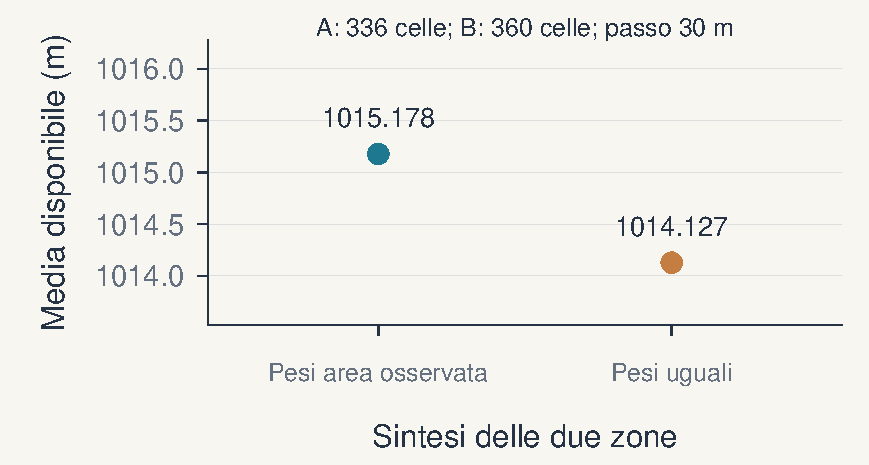
\includegraphics[width=9.85cm,height=5.25cm,keepaspectratio]{Risultati/Figure/34_pesi_aree.pdf}
\vspace{1.5mm}
\PSmall{Dopo la maschera restano 336 celle in A e 360 in B. Pesare per area osservata ricostruisce la media delle 696 celle disponibili.}
\[\overline z_A=\frac{\sum_b A_b\,\overline z_b}{\sum_b A_b}\]

\end{minipage}\end{lrbox}
\typeout{FULLBOX:093:PilotLeftBox:\the\ht\PilotLeftBox:\the\dp\PilotLeftBox}

\begin{lrbox}{\PilotRightBox}
\begin{minipage}[t]{7.55cm}\raggedright\color{Ink}\fontsize{11.3}{14.8}\selectfont
\PBody{Con zone della stessa area e copertura completa, media semplice delle medie e media per area coincidono. Non è una proprietà generale.}
\vspace{2.5mm}
\PInfo{La formula richiede che le medie zonali rappresentino le aree assegnate. Una copertura incompleta può richiedere un trattamento aggiuntivo.}
\PBody{La definizione dei pesi segue la domanda scientifica.}
\vspace{2.5mm}

\end{minipage}\end{lrbox}
\typeout{FULLBOX:093:PilotRightBox:\the\ht\PilotRightBox:\the\dp\PilotRightBox}

\begin{tikzpicture}[remember picture,overlay]
\PilotChrome{La media del territorio richiede pesi coerenti}{VIII · SINTESI TERRITORIALI}{93}{Il peso di una zona deve essere dichiarato insieme alla popolazione o al territorio che rappresenta.}
\node[anchor=north west,inner sep=0] at([xshift=.96cm,yshift=-2.13cm]current page.north west){\usebox{\PilotLeftBox}};
\node[anchor=north west,inner sep=0] at([xshift=11.52cm,yshift=-2.13cm]current page.north west){\usebox{\PilotRightBox}};
\node[anchor=north east,inner sep=0] at([xshift=17.65cm,yshift=-12.06cm]current page.north west){\color{Classical}\fontsize{7.7}{9.2}\selectfont\href{../../03_Notebook_svolti/M12_Tessera/M12_N15.html}{M12\_N15 · notebook svolto}};
\end{tikzpicture}\end{frame}

\begin{frame}[plain]\hypertarget{slide94}{}
\bookmark[level=1,page=94]{La copertura può differire fra le zone}
\begin{lrbox}{\TitleBox}
\begin{minipage}[t]{17.7cm}\raggedright\color{Ink}\fontsize{11.3}{14.8}\selectfont
\color{Navy}\bfseries\fontsize{20.6}{24.5}\selectfont La copertura può differire fra le zone
\end{minipage}\end{lrbox}
\typeout{FULLBOX:094:TitleBox:\the\ht\TitleBox:\the\dp\TitleBox}

\begin{lrbox}{\RecallBox}
\begin{minipage}[t]{14.3cm}\raggedright\color{Ink}\fontsize{11.3}{14.8}\selectfont
\fontsize{10.3}{13.8}\selectfont La copertura globale deve essere accompagnata dalla sua distribuzione nel territorio.
\end{minipage}\end{lrbox}
\typeout{FULLBOX:094:RecallBox:\the\ht\RecallBox:\the\dp\RecallBox}

\begin{lrbox}{\PilotLeftBox}
\begin{minipage}[t]{10.05cm}\raggedright\color{Ink}\fontsize{11.3}{14.8}\selectfont
{\fontsize{10.2}{13.1}\selectfont\renewcommand{\arraystretch}{1.45}\begin{tabular}{@{}p{3.0cm}p{3.2cm}p{2.4cm}@{}}\toprule
\textbf{Zona} & \textbf{Celle disponibili} & \textbf{Copertura}\\\midrule
A dopo la maschera & 336 su 360 & 93,33\%\\
B dopo la maschera & 360 su 360 & 100\%\\
Intero dominio & 696 su 720 & 96,67\%\\
\bottomrule\end{tabular}}

\end{minipage}\end{lrbox}
\typeout{FULLBOX:094:PilotLeftBox:\the\ht\PilotLeftBox:\the\dp\PilotLeftBox}

\begin{lrbox}{\PilotRightBox}
\begin{minipage}[t]{7.55cm}\raggedright\color{Ink}\fontsize{11.3}{14.8}\selectfont
\PBody{La finestra mancante cade interamente nella zona A. La stessa percentuale globale nasconde quindi una distribuzione geografica asimmetrica delle esclusioni.}
\vspace{2.5mm}
\PInfo{Confrontiamo medie zonali e coperture prima di interpretare la differenza fra A e B.}
\PCode{R · copertura per zona}{094_esempio.R}
\end{minipage}\end{lrbox}
\typeout{FULLBOX:094:PilotRightBox:\the\ht\PilotRightBox:\the\dp\PilotRightBox}

\begin{tikzpicture}[remember picture,overlay]
\PilotChrome{La copertura può differire fra le zone}{VIII · SINTESI TERRITORIALI}{94}{La copertura globale deve essere accompagnata dalla sua distribuzione nel territorio.}
\node[anchor=north west,inner sep=0] at([xshift=.96cm,yshift=-2.13cm]current page.north west){\usebox{\PilotLeftBox}};
\node[anchor=north west,inner sep=0] at([xshift=11.52cm,yshift=-2.13cm]current page.north west){\usebox{\PilotRightBox}};
\node[anchor=north east,inner sep=0] at([xshift=17.65cm,yshift=-12.06cm]current page.north west){\color{Classical}\fontsize{7.7}{9.2}\selectfont\href{../../03_Notebook_svolti/M12_Tessera/M12_N15.html}{M12\_N15 · notebook svolto}};
\end{tikzpicture}\end{frame}

\begin{frame}[plain]\hypertarget{slide95}{}
\bookmark[level=1,page=95]{Molti pixel non sono molte repliche indipendenti}
\begin{lrbox}{\TitleBox}
\begin{minipage}[t]{17.7cm}\raggedright\color{Ink}\fontsize{11.3}{14.8}\selectfont
\color{Navy}\bfseries\fontsize{20.6}{24.5}\selectfont Molti pixel non sono molte repliche indipendenti
\end{minipage}\end{lrbox}
\typeout{FULLBOX:095:TitleBox:\the\ht\TitleBox:\the\dp\TitleBox}

\begin{lrbox}{\RecallBox}
\begin{minipage}[t]{14.3cm}\raggedright\color{Ink}\fontsize{11.3}{14.8}\selectfont
\fontsize{10.3}{13.8}\selectfont La numerosità del file non determina automaticamente la quantità di informazione indipendente.
\end{minipage}\end{lrbox}
\typeout{FULLBOX:095:RecallBox:\the\ht\RecallBox:\the\dp\RecallBox}

\begin{lrbox}{\PilotLeftBox}
\begin{minipage}[t]{10.05cm}\raggedright\color{Ink}\fontsize{11.3}{14.8}\selectfont
{\fontsize{10.2}{13.1}\selectfont\renewcommand{\arraystretch}{1.45}\begin{tabular}{@{}p{4.2cm}p{4.8cm}@{}}\toprule
\textbf{Conteggio} & \textbf{Significato}\\\midrule
720 celle & Dimensione della griglia\\
64,8 ettari & Area piana del dominio\\
2 zone & Unità della tabella aggregata\\
12 blocchi didattici & Unità dello schema di ricampionamento\\
Repliche indipendenti & Proprietà del disegno o del modello\\
\bottomrule\end{tabular}}

\end{minipage}\end{lrbox}
\typeout{FULLBOX:095:PilotLeftBox:\the\ht\PilotLeftBox:\the\dp\PilotLeftBox}

\begin{lrbox}{\PilotRightBox}
\begin{minipage}[t]{7.55cm}\raggedright\color{Ink}\fontsize{11.3}{14.8}\selectfont
\PBody{La continuità della superficie crea relazioni fra celle vicine. Un test che tratta ogni pixel come una replica indipendente richiederebbe una giustificazione specifica.}
\vspace{2.5mm}
\PInfo{La differenza descrittiva fra le quote di A e B è calcolabile. L’inferenza su un processo o su altri territori richiede ipotesi ulteriori.}
\PBody{Le categorie del conteggio non devono essere confuse fra loro.}
\vspace{2.5mm}

\end{minipage}\end{lrbox}
\typeout{FULLBOX:095:PilotRightBox:\the\ht\PilotRightBox:\the\dp\PilotRightBox}

\begin{tikzpicture}[remember picture,overlay]
\PilotChrome{Molti pixel non sono molte repliche indipendenti}{VIII · SINTESI TERRITORIALI}{95}{La numerosità del file non determina automaticamente la quantità di informazione indipendente.}
\node[anchor=north west,inner sep=0] at([xshift=.96cm,yshift=-2.13cm]current page.north west){\usebox{\PilotLeftBox}};
\node[anchor=north west,inner sep=0] at([xshift=11.52cm,yshift=-2.13cm]current page.north west){\usebox{\PilotRightBox}};
\end{tikzpicture}\end{frame}

\begin{frame}[plain]\hypertarget{slide96}{}
\bookmark[level=1,page=96]{Le differenze a distanza descrivono due scale}
\begin{lrbox}{\TitleBox}
\begin{minipage}[t]{17.7cm}\raggedright\color{Ink}\fontsize{11.3}{14.8}\selectfont
\color{Navy}\bfseries\fontsize{20.6}{24.5}\selectfont Le differenze a distanza descrivono due scale
\end{minipage}\end{lrbox}
\typeout{FULLBOX:096:TitleBox:\the\ht\TitleBox:\the\dp\TitleBox}

\begin{lrbox}{\RecallBox}
\begin{minipage}[t]{14.3cm}\raggedright\color{Ink}\fontsize{11.3}{14.8}\selectfont
\fontsize{10.3}{13.8}\selectfont La distanza delle coppie e il loro riuso delle celle devono accompagnare la statistica.
\end{minipage}\end{lrbox}
\typeout{FULLBOX:096:RecallBox:\the\ht\RecallBox:\the\dp\RecallBox}

\begin{lrbox}{\PilotLeftBox}
\begin{minipage}[t]{10.05cm}\raggedright\color{Ink}\fontsize{11.3}{14.8}\selectfont
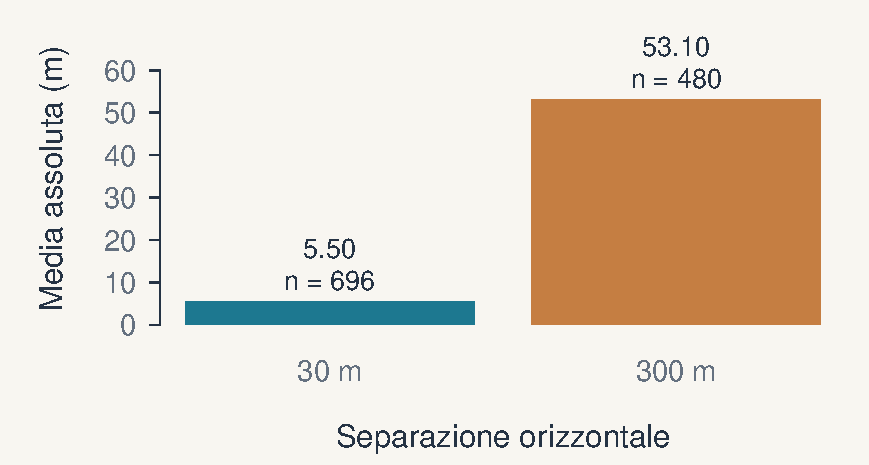
\includegraphics[width=9.85cm,height=5.25cm,keepaspectratio]{Risultati/Figure/35_differenze30_300.pdf}
\vspace{1.5mm}
\PSmall{Differenze longitudinali a 30 m e 300 m: 696 e 480 coppie rispettivamente, costruite nella stessa superficie.}

\end{minipage}\end{lrbox}
\typeout{FULLBOX:096:PilotLeftBox:\the\ht\PilotLeftBox:\the\dp\PilotLeftBox}

\begin{lrbox}{\PilotRightBox}
\begin{minipage}[t]{7.55cm}\raggedright\color{Ink}\fontsize{11.3}{14.8}\selectfont
\PBody{Le coppie possono condividere celle e risentono della tendenza del terreno. Il confronto descrive come cambia il campo a due separazioni.}
\vspace{2.5mm}
\PInfo{Non presentiamo i contributi come repliche indipendenti né il confronto come un test causale.}
\PCode{R · due separazioni spaziali}{096_esempio.R}
\end{minipage}\end{lrbox}
\typeout{FULLBOX:096:PilotRightBox:\the\ht\PilotRightBox:\the\dp\PilotRightBox}

\begin{tikzpicture}[remember picture,overlay]
\PilotChrome{Le differenze a distanza descrivono due scale}{VIII · SINTESI TERRITORIALI}{96}{La distanza delle coppie e il loro riuso delle celle devono accompagnare la statistica.}
\node[anchor=north west,inner sep=0] at([xshift=.96cm,yshift=-2.13cm]current page.north west){\usebox{\PilotLeftBox}};
\node[anchor=north west,inner sep=0] at([xshift=11.52cm,yshift=-2.13cm]current page.north west){\usebox{\PilotRightBox}};
\node[anchor=north east,inner sep=0] at([xshift=17.65cm,yshift=-12.06cm]current page.north west){\color{Classical}\fontsize{7.7}{9.2}\selectfont\href{../../03_Notebook_svolti/M12_Tessera/M12_N16.html}{M12\_N16 · notebook svolto}};
\end{tikzpicture}\end{frame}

\begin{frame}[plain]\hypertarget{slide97}{}
\bookmark[level=1,page=97]{La varianza della media include le covarianze}
\begin{lrbox}{\TitleBox}
\begin{minipage}[t]{17.7cm}\raggedright\color{Ink}\fontsize{11.3}{14.8}\selectfont
\color{Navy}\bfseries\fontsize{20.6}{24.5}\selectfont La varianza della media include le covarianze
\end{minipage}\end{lrbox}
\typeout{FULLBOX:097:TitleBox:\the\ht\TitleBox:\the\dp\TitleBox}

\begin{lrbox}{\RecallBox}
\begin{minipage}[t]{14.3cm}\raggedright\color{Ink}\fontsize{11.3}{14.8}\selectfont
\fontsize{10.3}{13.8}\selectfont L’incertezza va riferita a un bersaglio e a un meccanismo di variazione espliciti.
\end{minipage}\end{lrbox}
\typeout{FULLBOX:097:RecallBox:\the\ht\RecallBox:\the\dp\RecallBox}

\begin{lrbox}{\PilotLeftBox}
\begin{minipage}[t]{10.05cm}\raggedright\color{Ink}\fontsize{11.3}{14.8}\selectfont
\[\operatorname{Var}(\overline Z)
 =\frac1{n^2}\sum_i\sum_j\operatorname{Cov}(Z_i,Z_j)\]
\[=\frac1{n^2}\left\{\sum_i\operatorname{Var}(Z_i)
       +2\sum_{i<j}\operatorname{Cov}(Z_i,Z_j)\right\}\]
\PInfo{La relazione riguarda variabili aleatorie. Una superficie sintetica completamente nota ha una media finita calcolabile senza errore di campionamento.}

\end{minipage}\end{lrbox}
\typeout{FULLBOX:097:PilotLeftBox:\the\ht\PilotLeftBox:\the\dp\PilotLeftBox}

\begin{lrbox}{\PilotRightBox}
\begin{minipage}[t]{7.55cm}\raggedright\color{Ink}\fontsize{11.3}{14.8}\selectfont
\PBody{Per discutere l’incertezza su un processo o su territori non osservati serve un modello o un disegno che definisca la variabilità.}
\vspace{2.5mm}
\PBody{Il rapporto fra numero di celle e precisione non dipende soltanto dalla varianza marginale. Le covarianze possono contribuire in modo sostanziale.}
\vspace{2.5mm}

\end{minipage}\end{lrbox}
\typeout{FULLBOX:097:PilotRightBox:\the\ht\PilotRightBox:\the\dp\PilotRightBox}

\begin{tikzpicture}[remember picture,overlay]
\PilotChrome{La varianza della media include le covarianze}{VIII · SINTESI TERRITORIALI}{97}{L’incertezza va riferita a un bersaglio e a un meccanismo di variazione espliciti.}
\node[anchor=north west,inner sep=0] at([xshift=.96cm,yshift=-2.13cm]current page.north west){\usebox{\PilotLeftBox}};
\node[anchor=north west,inner sep=0] at([xshift=11.52cm,yshift=-2.13cm]current page.north west){\usebox{\PilotRightBox}};
\end{tikzpicture}\end{frame}

\begin{frame}[plain]\hypertarget{slide98}{}
\bookmark[level=1,page=98]{Il ricampionamento a blocchi dichiara nuove unità}
\begin{lrbox}{\TitleBox}
\begin{minipage}[t]{17.7cm}\raggedright\color{Ink}\fontsize{11.3}{14.8}\selectfont
\color{Navy}\bfseries\fontsize{20.6}{24.5}\selectfont Il ricampionamento a blocchi dichiara nuove unità
\end{minipage}\end{lrbox}
\typeout{FULLBOX:098:TitleBox:\the\ht\TitleBox:\the\dp\TitleBox}

\begin{lrbox}{\RecallBox}
\begin{minipage}[t]{14.3cm}\raggedright\color{Ink}\fontsize{11.3}{14.8}\selectfont
\fontsize{10.3}{13.8}\selectfont Lo schema di ricampionamento deve essere descritto nella geometria e nei pesi.
\end{minipage}\end{lrbox}
\typeout{FULLBOX:098:RecallBox:\the\ht\RecallBox:\the\dp\RecallBox}

\begin{lrbox}{\PilotLeftBox}
\begin{minipage}[t]{10.05cm}\raggedright\color{Ink}\fontsize{11.3}{14.8}\selectfont
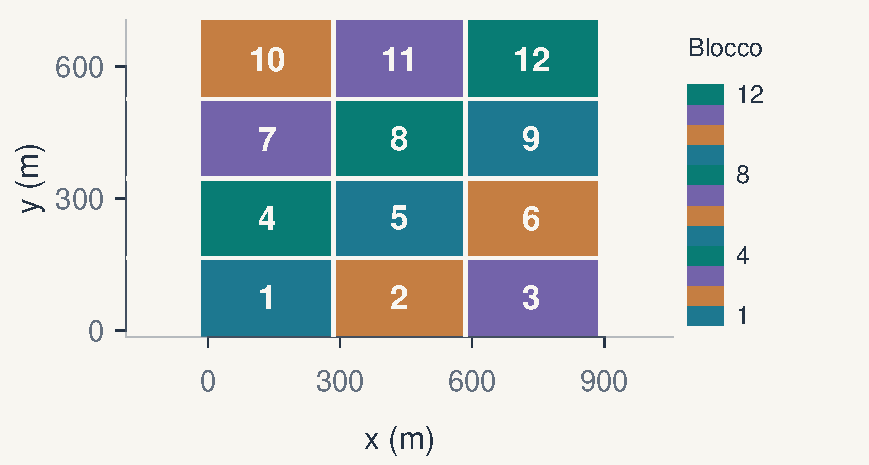
\includegraphics[width=9.85cm,height=5.25cm,keepaspectratio]{Risultati/Figure/36_blocchi12.pdf}
\vspace{1.5mm}
\PSmall{Dodici blocchi contigui: 6 righe e 10 colonne ciascuno, 60 celle e 5,4 ha di area piana per blocco.}

\end{minipage}\end{lrbox}
\typeout{FULLBOX:098:PilotLeftBox:\the\ht\PilotLeftBox:\the\dp\PilotLeftBox}

\begin{lrbox}{\PilotRightBox}
\begin{minipage}[t]{7.55cm}\raggedright\color{Ink}\fontsize{11.3}{14.8}\selectfont
\PBody{Calcoliamo la media di ciascun blocco. Ricampioniamo poi dodici medie con reinserimento per ottenere una nuova media complessiva.}
\vspace{2.5mm}
\PInfo{I blocchi sono completi ed equiponderati: la media delle dodici medie coincide con quella delle 720 quote.}
\PCode{R · controllare il bersaglio}{098_esempio.R}
\end{minipage}\end{lrbox}
\typeout{FULLBOX:098:PilotRightBox:\the\ht\PilotRightBox:\the\dp\PilotRightBox}

\begin{tikzpicture}[remember picture,overlay]
\PilotChrome{Il ricampionamento a blocchi dichiara nuove unità}{VIII · SINTESI TERRITORIALI}{98}{Lo schema di ricampionamento deve essere descritto nella geometria e nei pesi.}
\node[anchor=north west,inner sep=0] at([xshift=.96cm,yshift=-2.13cm]current page.north west){\usebox{\PilotLeftBox}};
\node[anchor=north west,inner sep=0] at([xshift=11.52cm,yshift=-2.13cm]current page.north west){\usebox{\PilotRightBox}};
\node[anchor=north east,inner sep=0] at([xshift=17.65cm,yshift=-12.06cm]current page.north west){\color{Classical}\fontsize{7.7}{9.2}\selectfont\href{../../03_Notebook_svolti/M12_Tessera/M12_N17.html}{M12\_N17 · notebook svolto}};
\end{tikzpicture}\end{frame}

\begin{frame}[plain]\hypertarget{slide99}{}
\bookmark[level=1,page=99]{Due distribuzioni da ricampionamento}
\begin{lrbox}{\TitleBox}
\begin{minipage}[t]{17.7cm}\raggedright\color{Ink}\fontsize{11.3}{14.8}\selectfont
\color{Navy}\bfseries\fontsize{20.6}{24.5}\selectfont Due distribuzioni da ricampionamento
\end{minipage}\end{lrbox}
\typeout{FULLBOX:099:TitleBox:\the\ht\TitleBox:\the\dp\TitleBox}

\begin{lrbox}{\RecallBox}
\begin{minipage}[t]{14.3cm}\raggedright\color{Ink}\fontsize{11.3}{14.8}\selectfont
\fontsize{10.3}{13.8}\selectfont Aumentare le repliche rende più preciso il calcolo dello schema scelto, non rende automaticamente valido lo schema.
\end{minipage}\end{lrbox}
\typeout{FULLBOX:099:RecallBox:\the\ht\RecallBox:\the\dp\RecallBox}

\begin{lrbox}{\FullWideBox}
\begin{minipage}[t]{18.1cm}\raggedright\color{Ink}\fontsize{11.3}{14.8}\selectfont
\centering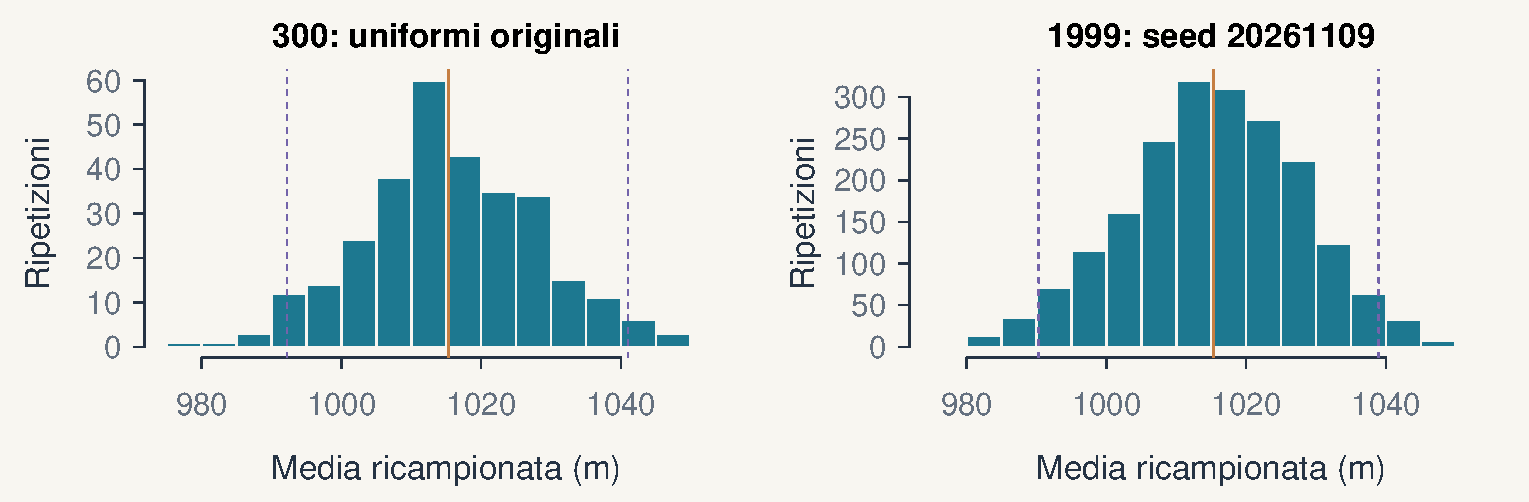
\includegraphics[width=18.05cm,height=5.8cm,keepaspectratio]{Risultati/Figure/37_bootstrap300_1999.pdf}
\end{minipage}\end{lrbox}
\typeout{FULLBOX:099:FullWideBox:\the\ht\FullWideBox:\the\dp\FullWideBox}

\begin{lrbox}{\PilotRightBox}
\begin{minipage}[t]{18.1cm}\raggedright\color{Ink}\fontsize{11.3}{14.8}\selectfont
\PBody{Dodici medie di blocco ricampionate con reinserimento. La serie di 300 repliche usa i numeri uniformi comuni del laboratorio originale; quella di 1999 usa il seme documentato della figura originale. I quantili descrivono queste distribuzioni condizionate allo schema. Il numero di repliche cambia la precisione Monte Carlo, non giustifica le ipotesi inferenziali.}
\end{minipage}\end{lrbox}
\typeout{FULLBOX:099:PilotRightBox:\the\ht\PilotRightBox:\the\dp\PilotRightBox}

\begin{tikzpicture}[remember picture,overlay]
\PilotChrome{Due distribuzioni da ricampionamento}{VIII · SINTESI TERRITORIALI}{99}{Aumentare le repliche rende più preciso il calcolo dello schema scelto, non rende automaticamente valido lo schema.}
\node[anchor=north west,inner sep=0] at([xshift=.96cm,yshift=-2.13cm]current page.north west){\usebox{\FullWideBox}};
\node[anchor=north west,inner sep=0] at([xshift=.96cm,yshift=-8.25cm]current page.north west){\usebox{\PilotRightBox}};
\node[anchor=north east,inner sep=0] at([xshift=17.65cm,yshift=-12.06cm]current page.north west){\color{Classical}\fontsize{7.7}{9.2}\selectfont\href{../../03_Notebook_svolti/M12_Tessera/M12_N17.html}{M12\_N17 · notebook svolto}};
\end{tikzpicture}\end{frame}

\begin{frame}[plain]\hypertarget{slide100}{}
\bookmark[level=1,page=100]{Il bersaglio guida la scelta dei blocchi}
\begin{lrbox}{\TitleBox}
\begin{minipage}[t]{17.7cm}\raggedright\color{Ink}\fontsize{11.3}{14.8}\selectfont
\color{Navy}\bfseries\fontsize{20.6}{24.5}\selectfont Il bersaglio guida la scelta dei blocchi
\end{minipage}\end{lrbox}
\typeout{FULLBOX:100:TitleBox:\the\ht\TitleBox:\the\dp\TitleBox}

\begin{lrbox}{\RecallBox}
\begin{minipage}[t]{14.3cm}\raggedright\color{Ink}\fontsize{11.3}{14.8}\selectfont
\fontsize{10.3}{13.8}\selectfont Le ipotesi del ricampionamento devono essere motivate rispetto a dipendenza, tendenza e popolazione.
\end{minipage}\end{lrbox}
\typeout{FULLBOX:100:RecallBox:\the\ht\RecallBox:\the\dp\RecallBox}

\begin{lrbox}{\PilotLeftBox}
\begin{minipage}[t]{10.05cm}\raggedright\color{Ink}\fontsize{11.3}{14.8}\selectfont
\[\overline Z^*=\frac1{12}\sum_{b=1}^{12}\overline Z_{J_b},
 \qquad J_b\overset{\mathrm{iid}}{\sim}\operatorname{Unif}\{1,\ldots,12\}\]
\PInfo{L’indipendenza riguarda le estrazioni degli indici nello schema bootstrap. Non dimostra che i dodici blocchi del terreno siano indipendenti o scambiabili.}

\end{minipage}\end{lrbox}
\typeout{FULLBOX:100:PilotLeftBox:\the\ht\PilotLeftBox:\the\dp\PilotLeftBox}

\begin{lrbox}{\PilotRightBox}
\begin{minipage}[t]{7.55cm}\raggedright\color{Ink}\fontsize{11.3}{14.8}\selectfont
\PBody{Blocchi vicini possono restare dipendenti. Un gradiente può rendere le loro distribuzioni diverse.}
\vspace{2.5mm}
\PBody{Nel caso didattico i quantili sono un’analisi di sensibilità allo schema, non un intervallo con copertura garantita per una popolazione geografica non definita.}
\vspace{2.5mm}

\end{minipage}\end{lrbox}
\typeout{FULLBOX:100:PilotRightBox:\the\ht\PilotRightBox:\the\dp\PilotRightBox}

\begin{tikzpicture}[remember picture,overlay]
\PilotChrome{Il bersaglio guida la scelta dei blocchi}{VIII · SINTESI TERRITORIALI}{100}{Le ipotesi del ricampionamento devono essere motivate rispetto a dipendenza, tendenza e popolazione.}
\node[anchor=north west,inner sep=0] at([xshift=.96cm,yshift=-2.13cm]current page.north west){\usebox{\PilotLeftBox}};
\node[anchor=north west,inner sep=0] at([xshift=11.52cm,yshift=-2.13cm]current page.north west){\usebox{\PilotRightBox}};
\node[anchor=north east,inner sep=0] at([xshift=17.65cm,yshift=-12.06cm]current page.north west){\color{Classical}\fontsize{7.7}{9.2}\selectfont\href{../../03_Notebook_svolti/M12_Tessera/M12_N17.html}{M12\_N17 · notebook svolto}};
\end{tikzpicture}\end{frame}

\begin{frame}[plain]\hypertarget{slide101}{}
\bookmark[level=1,page=101]{Cambia l’unità, cambia il risultato}
\begin{lrbox}{\TitleBox}
\begin{minipage}[t]{17.7cm}\raggedright\color{Ink}\fontsize{11.3}{14.8}\selectfont
\color{Navy}\bfseries\fontsize{20.6}{24.5}\selectfont Cambia l’unità, cambia il risultato
\end{minipage}\end{lrbox}
\typeout{FULLBOX:101:TitleBox:\the\ht\TitleBox:\the\dp\TitleBox}

\begin{lrbox}{\RecallBox}
\begin{minipage}[t]{14.3cm}\raggedright\color{Ink}\fontsize{11.3}{14.8}\selectfont
\fontsize{10.3}{13.8}\selectfont Il confronto fra schemi serve a esaminare le assunzioni, non a scegliere il risultato più conveniente.
\end{minipage}\end{lrbox}
\typeout{FULLBOX:101:RecallBox:\the\ht\RecallBox:\the\dp\RecallBox}

\begin{lrbox}{\PilotLeftBox}
\begin{minipage}[t]{10.05cm}\raggedright\color{Ink}\fontsize{11.3}{14.8}\selectfont
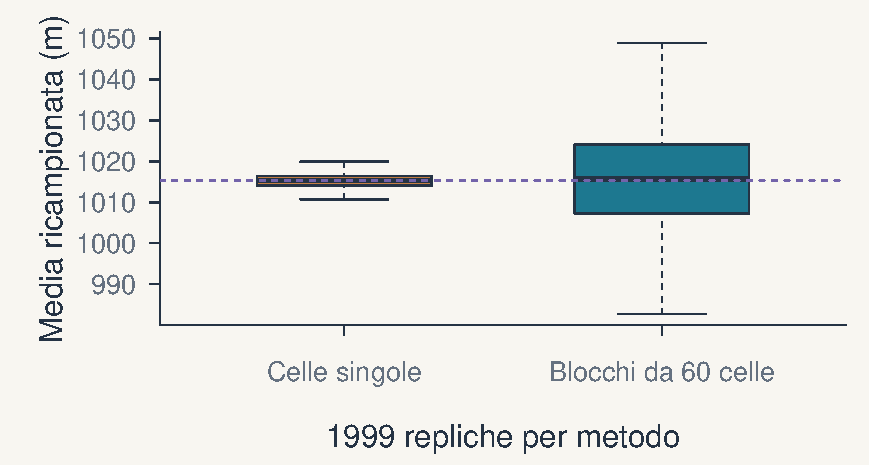
\includegraphics[width=9.85cm,height=5.25cm,keepaspectratio]{Risultati/Figure/38_bootstrap_confronto.pdf}
\vspace{1.5mm}
\PSmall{Confronto fra schemi di ricampionamento. Le distribuzioni riflettono la scelta delle unità e delle ipotesi.}

\end{minipage}\end{lrbox}
\typeout{FULLBOX:101:PilotLeftBox:\the\ht\PilotLeftBox:\the\dp\PilotLeftBox}

\begin{lrbox}{\PilotRightBox}
\begin{minipage}[t]{7.55cm}\raggedright\color{Ink}\fontsize{11.3}{14.8}\selectfont
\PBody{Ricampionare singole celle rompe le relazioni locali. Ricampionare blocchi conserva parte della struttura, ma introduce scelte su forma, dimensione e disposizione.}
\vspace{2.5mm}
\PInfo{Un intervallo più ampio non è automaticamente corretto. La validità richiede che il meccanismo rappresenti l’incertezza del compito.}
\PBody{I registri conservano parametri, semi e quantili per rendere verificabile la sensibilità.}
\vspace{2.5mm}

\end{minipage}\end{lrbox}
\typeout{FULLBOX:101:PilotRightBox:\the\ht\PilotRightBox:\the\dp\PilotRightBox}

\begin{tikzpicture}[remember picture,overlay]
\PilotChrome{Cambia l’unità, cambia il risultato}{VIII · SINTESI TERRITORIALI}{101}{Il confronto fra schemi serve a esaminare le assunzioni, non a scegliere il risultato più conveniente.}
\node[anchor=north west,inner sep=0] at([xshift=.96cm,yshift=-2.13cm]current page.north west){\usebox{\PilotLeftBox}};
\node[anchor=north west,inner sep=0] at([xshift=11.52cm,yshift=-2.13cm]current page.north west){\usebox{\PilotRightBox}};
\node[anchor=north east,inner sep=0] at([xshift=17.65cm,yshift=-12.06cm]current page.north west){\color{Classical}\fontsize{7.7}{9.2}\selectfont\href{../../03_Notebook_svolti/M12_Tessera/M12_N17.html}{M12\_N17 · notebook svolto}};
\end{tikzpicture}\end{frame}

\begin{frame}[plain]\hypertarget{slide102}{}
\bookmark[level=1,page=102]{Laboratorio: collegare sintesi, dominio e ipotesi}
\begin{lrbox}{\TitleBox}
\begin{minipage}[t]{17.7cm}\raggedright\color{Ink}\fontsize{11.3}{14.8}\selectfont
\color{Navy}\bfseries\fontsize{20.6}{24.5}\selectfont Laboratorio: collegare sintesi, dominio e ipotesi
\end{minipage}\end{lrbox}
\typeout{FULLBOX:102:TitleBox:\the\ht\TitleBox:\the\dp\TitleBox}

\begin{lrbox}{\RecallBox}
\begin{minipage}[t]{14.3cm}\raggedright\color{Ink}\fontsize{11.3}{14.8}\selectfont
\fontsize{10.3}{13.8}\selectfont Una sintesi territoriale resta scientificamente leggibile quando conserva dominio, unità e assunzioni.
\end{minipage}\end{lrbox}
\typeout{FULLBOX:102:RecallBox:\the\ht\RecallBox:\the\dp\RecallBox}

\begin{lrbox}{\PilotLeftBox}
\begin{minipage}[t]{10.05cm}\raggedright\color{Ink}\fontsize{11.3}{14.8}\selectfont
\PLab{https://marzione00.github.io/Lab_Geo/\#laboratorio/m12-zone}{Esperimento online · sintesi zonali}
{\fontsize{10.2}{13.1}\selectfont\renewcommand{\arraystretch}{1.45}\begin{tabular}{@{}p{4.1cm}p{4.9cm}@{}}\toprule
\textbf{Attività} & \textbf{Evidenza}\\\midrule
N15: zone & Medie, dispersione, conteggi e copertura\\
N16: distanze & Coppie a 30 e 300 m\\
N17: blocchi & Geometria e regola di ricampionamento\\
Confronto & Sensibilità alle unità scelte\\
Conclusione & Bersaglio e limiti dell’inferenza\\
\bottomrule\end{tabular}}

\end{minipage}\end{lrbox}
\typeout{FULLBOX:102:PilotLeftBox:\the\ht\PilotLeftBox:\the\dp\PilotLeftBox}

\begin{lrbox}{\PilotRightBox}
\begin{minipage}[t]{7.55cm}\raggedright\color{Ink}\fontsize{11.3}{14.8}\selectfont
\PBody{La tabella finale mantiene il legame con la mappa. Ogni media indica quali celle rappresenta e con quali pesi.}
\vspace{2.5mm}
\PInfo{Il processo di esportazione conserverà queste decisioni insieme ai raster e ai risultati numerici.}

\end{minipage}\end{lrbox}
\typeout{FULLBOX:102:PilotRightBox:\the\ht\PilotRightBox:\the\dp\PilotRightBox}

\begin{tikzpicture}[remember picture,overlay]
\PilotChrome{Laboratorio: collegare sintesi, dominio e ipotesi}{VIII · SINTESI TERRITORIALI}{102}{Una sintesi territoriale resta scientificamente leggibile quando conserva dominio, unità e assunzioni.}
\node[anchor=north west,inner sep=0] at([xshift=.96cm,yshift=-2.13cm]current page.north west){\usebox{\PilotLeftBox}};
\node[anchor=north west,inner sep=0] at([xshift=11.52cm,yshift=-2.13cm]current page.north west){\usebox{\PilotRightBox}};
\node[anchor=north east,inner sep=0] at([xshift=17.65cm,yshift=-12.06cm]current page.north west){\color{Classical}\fontsize{7.7}{9.2}\selectfont\href{../../03_Notebook_svolti/M12_Tessera/M12_N17.html}{M12\_N17 · notebook svolto}};
\end{tikzpicture}\end{frame}

\begin{frame}[plain]\hypertarget{slide103}{}
\bookmark[level=0,page=103]{IX · CONSEGNA E VERIFICA}
\bookmark[level=1,page=103]{La memoria cresce con celle, bande e precisione}
\begin{lrbox}{\TitleBox}
\begin{minipage}[t]{17.7cm}\raggedright\color{Ink}\fontsize{11.3}{14.8}\selectfont
\color{Navy}\bfseries\fontsize{20.6}{24.5}\selectfont La memoria cresce con celle, bande e precisione
\end{minipage}\end{lrbox}
\typeout{FULLBOX:103:TitleBox:\the\ht\TitleBox:\the\dp\TitleBox}

\begin{lrbox}{\RecallBox}
\begin{minipage}[t]{14.3cm}\raggedright\color{Ink}\fontsize{11.3}{14.8}\selectfont
\fontsize{10.3}{13.8}\selectfont La strategia di memoria deve essere dimensionata prima di materializzare grandi array.
\end{minipage}\end{lrbox}
\typeout{FULLBOX:103:RecallBox:\the\ht\RecallBox:\the\dp\RecallBox}

\begin{lrbox}{\PilotLeftBox}
\begin{minipage}[t]{10.05cm}\raggedright\color{Ink}\fontsize{11.3}{14.8}\selectfont
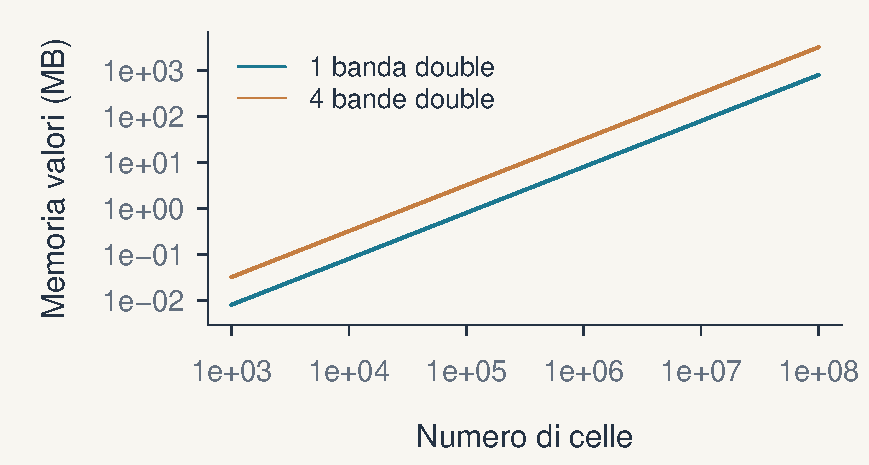
\includegraphics[width=9.85cm,height=5.25cm,keepaspectratio]{Risultati/Figure/39_memoria.pdf}
\vspace{1.5mm}
\PSmall{Dimensione teorica dei valori numerici. File compresso, oggetti in memoria e copie temporanee hanno costi differenti.}
\[B=n_r\,n_c\,n_b\,q\]

\end{minipage}\end{lrbox}
\typeout{FULLBOX:103:PilotLeftBox:\the\ht\PilotLeftBox:\the\dp\PilotLeftBox}

\begin{lrbox}{\PilotRightBox}
\begin{minipage}[t]{7.55cm}\raggedright\color{Ink}\fontsize{11.3}{14.8}\selectfont
\PBody{$q$ è il numero di byte per valore. Dimezzare il passo su entrambi gli assi quadruplica le celle sullo stesso dominio.}
\vspace{2.5mm}
\PInfo{La formula conta soltanto i valori: non include metadati, maschere, indici e copie temporanee. Aprire un SpatRaster non carica automaticamente tutti i pixel.}
\PCode{R · stima senza allocazione}{103_esempio.R}
\end{minipage}\end{lrbox}
\typeout{FULLBOX:103:PilotRightBox:\the\ht\PilotRightBox:\the\dp\PilotRightBox}

\begin{tikzpicture}[remember picture,overlay]
\PilotChrome{La memoria cresce con celle, bande e precisione}{IX · CONSEGNA E VERIFICA}{103}{La strategia di memoria deve essere dimensionata prima di materializzare grandi array.}
\node[anchor=north west,inner sep=0] at([xshift=.96cm,yshift=-2.13cm]current page.north west){\usebox{\PilotLeftBox}};
\node[anchor=north west,inner sep=0] at([xshift=11.52cm,yshift=-2.13cm]current page.north west){\usebox{\PilotRightBox}};
\node[anchor=north east,inner sep=0] at([xshift=17.65cm,yshift=-12.06cm]current page.north west){\color{Classical}\fontsize{7.7}{9.2}\selectfont\href{../../03_Notebook_svolti/M12_Tessera/M12_N18.html}{M12\_N18 · notebook svolto}};
\end{tikzpicture}\end{frame}

\begin{frame}[plain]\hypertarget{slide104}{}
\bookmark[level=1,page=104]{Leggere una finestra conserva ordine e posizioni}
\begin{lrbox}{\TitleBox}
\begin{minipage}[t]{17.7cm}\raggedright\color{Ink}\fontsize{11.3}{14.8}\selectfont
\color{Navy}\bfseries\fontsize{20.6}{24.5}\selectfont Leggere una finestra conserva ordine e posizioni
\end{minipage}\end{lrbox}
\typeout{FULLBOX:104:TitleBox:\the\ht\TitleBox:\the\dp\TitleBox}

\begin{lrbox}{\RecallBox}
\begin{minipage}[t]{14.3cm}\raggedright\color{Ink}\fontsize{11.3}{14.8}\selectfont
\fontsize{10.3}{13.8}\selectfont Una lettura parziale deve restituire gli stessi valori e lo stesso ordine della porzione corrispondente.
\end{minipage}\end{lrbox}
\typeout{FULLBOX:104:RecallBox:\the\ht\RecallBox:\the\dp\RecallBox}

\begin{lrbox}{\PilotLeftBox}
\begin{minipage}[t]{10.05cm}\raggedright\color{Ink}\fontsize{11.3}{14.8}\selectfont
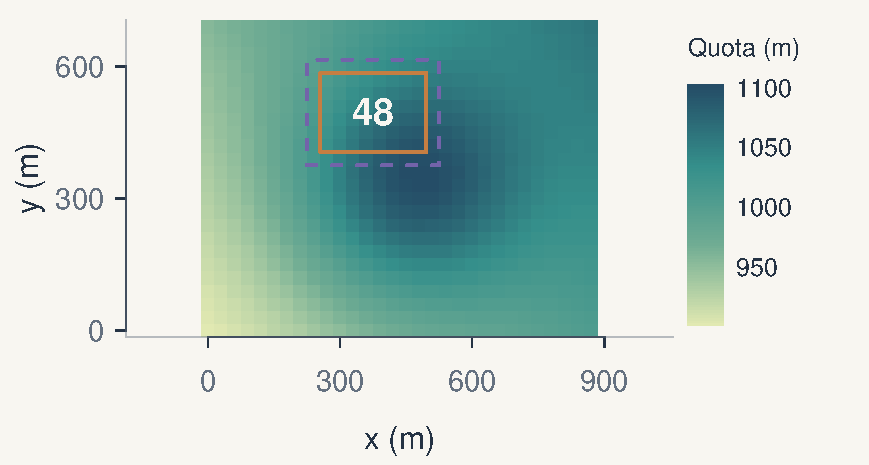
\includegraphics[width=9.85cm,height=5.25cm,keepaspectratio]{Risultati/Figure/40_finestra_halo.pdf}
\vspace{1.5mm}
\PSmall{La finestra centrale contiene 6×8 celle. Il contorno aggiuntivo permette di calcolare le derivate senza perdere i vicini.}

\end{minipage}\end{lrbox}
\typeout{FULLBOX:104:PilotLeftBox:\the\ht\PilotLeftBox:\the\dp\PilotLeftBox}

\begin{lrbox}{\PilotRightBox}
\begin{minipage}[t]{7.55cm}\raggedright\color{Ink}\fontsize{11.3}{14.8}\selectfont
\PBody{Leggiamo 48 valori dal GeoTIFF e li confrontiamo con le stesse celle della matrice completa.}
\vspace{2.5mm}
\PSmall{Questo riferimento completo è praticabile sul piccolo dataset didattico.}
\PCode{R · finestra realmente letta}{104_esempio.R}
\end{minipage}\end{lrbox}
\typeout{FULLBOX:104:PilotRightBox:\the\ht\PilotRightBox:\the\dp\PilotRightBox}

\begin{tikzpicture}[remember picture,overlay]
\PilotChrome{Leggere una finestra conserva ordine e posizioni}{IX · CONSEGNA E VERIFICA}{104}{Una lettura parziale deve restituire gli stessi valori e lo stesso ordine della porzione corrispondente.}
\node[anchor=north west,inner sep=0] at([xshift=.96cm,yshift=-2.13cm]current page.north west){\usebox{\PilotLeftBox}};
\node[anchor=north west,inner sep=0] at([xshift=11.52cm,yshift=-2.13cm]current page.north west){\usebox{\PilotRightBox}};
\node[anchor=north east,inner sep=0] at([xshift=17.65cm,yshift=-12.06cm]current page.north west){\color{Classical}\fontsize{7.7}{9.2}\selectfont\href{../../03_Notebook_svolti/M12_Tessera/M12_N18.html}{M12\_N18 · notebook svolto}};
\end{tikzpicture}\end{frame}

\begin{frame}[plain]\hypertarget{slide105}{}
\bookmark[level=1,page=105]{Le operazioni locali richiedono un bordo di lettura}
\begin{lrbox}{\TitleBox}
\begin{minipage}[t]{17.7cm}\raggedright\color{Ink}\fontsize{11.3}{14.8}\selectfont
\color{Navy}\bfseries\fontsize{20.6}{24.5}\selectfont Le operazioni locali richiedono un bordo di lettura
\end{minipage}\end{lrbox}
\typeout{FULLBOX:105:TitleBox:\the\ht\TitleBox:\the\dp\TitleBox}

\begin{lrbox}{\RecallBox}
\begin{minipage}[t]{14.3cm}\raggedright\color{Ink}\fontsize{11.3}{14.8}\selectfont
\fontsize{10.3}{13.8}\selectfont Ridurre la memoria deve preservare i vicinati necessari al procedimento scientifico.
\end{minipage}\end{lrbox}
\typeout{FULLBOX:105:RecallBox:\the\ht\RecallBox:\the\dp\RecallBox}

\begin{lrbox}{\PilotLeftBox}
\begin{minipage}[t]{10.05cm}\raggedright\color{Ink}\fontsize{11.3}{14.8}\selectfont
\begin{tikzpicture}[x=1cm,y=1cm]
\path[use as bounding box](-.1,-.15) rectangle(9.7,5.7);
\filldraw[fill=GeoB!23,draw=white](1.0,0.65)rectangle(1.65,1.1800000000000002);
\filldraw[fill=GeoB!23,draw=white](1.65,0.65)rectangle(2.3,1.1800000000000002);
\filldraw[fill=GeoB!23,draw=white](2.3,0.65)rectangle(2.9499999999999997,1.1800000000000002);
\filldraw[fill=GeoB!23,draw=white](2.95,0.65)rectangle(3.6,1.1800000000000002);
\filldraw[fill=GeoB!23,draw=white](3.6,0.65)rectangle(4.25,1.1800000000000002);
\filldraw[fill=GeoB!23,draw=white](4.25,0.65)rectangle(4.9,1.1800000000000002);
\filldraw[fill=GeoB!23,draw=white](4.9,0.65)rectangle(5.550000000000001,1.1800000000000002);
\filldraw[fill=GeoB!23,draw=white](5.55,0.65)rectangle(6.2,1.1800000000000002);
\filldraw[fill=GeoB!23,draw=white](6.2,0.65)rectangle(6.8500000000000005,1.1800000000000002);
\filldraw[fill=GeoB!23,draw=white](6.8500000000000005,0.65)rectangle(7.500000000000001,1.1800000000000002);
\filldraw[fill=GeoB!23,draw=white](1.0,1.1800000000000002)rectangle(1.65,1.7100000000000002);
\filldraw[fill=GeoA!17,draw=white](1.65,1.1800000000000002)rectangle(2.3,1.7100000000000002);
\filldraw[fill=GeoA!17,draw=white](2.3,1.1800000000000002)rectangle(2.9499999999999997,1.7100000000000002);
\filldraw[fill=GeoA!17,draw=white](2.95,1.1800000000000002)rectangle(3.6,1.7100000000000002);
\filldraw[fill=GeoA!17,draw=white](3.6,1.1800000000000002)rectangle(4.25,1.7100000000000002);
\filldraw[fill=GeoA!17,draw=white](4.25,1.1800000000000002)rectangle(4.9,1.7100000000000002);
\filldraw[fill=GeoA!17,draw=white](4.9,1.1800000000000002)rectangle(5.550000000000001,1.7100000000000002);
\filldraw[fill=GeoA!17,draw=white](5.55,1.1800000000000002)rectangle(6.2,1.7100000000000002);
\filldraw[fill=GeoA!17,draw=white](6.2,1.1800000000000002)rectangle(6.8500000000000005,1.7100000000000002);
\filldraw[fill=GeoB!23,draw=white](6.8500000000000005,1.1800000000000002)rectangle(7.500000000000001,1.7100000000000002);
\filldraw[fill=GeoB!23,draw=white](1.0,1.71)rectangle(1.65,2.24);
\filldraw[fill=GeoA!17,draw=white](1.65,1.71)rectangle(2.3,2.24);
\filldraw[fill=GeoA!17,draw=white](2.3,1.71)rectangle(2.9499999999999997,2.24);
\filldraw[fill=GeoA!17,draw=white](2.95,1.71)rectangle(3.6,2.24);
\filldraw[fill=GeoA!17,draw=white](3.6,1.71)rectangle(4.25,2.24);
\filldraw[fill=GeoA!17,draw=white](4.25,1.71)rectangle(4.9,2.24);
\filldraw[fill=GeoA!17,draw=white](4.9,1.71)rectangle(5.550000000000001,2.24);
\filldraw[fill=GeoA!17,draw=white](5.55,1.71)rectangle(6.2,2.24);
\filldraw[fill=GeoA!17,draw=white](6.2,1.71)rectangle(6.8500000000000005,2.24);
\filldraw[fill=GeoB!23,draw=white](6.8500000000000005,1.71)rectangle(7.500000000000001,2.24);
\filldraw[fill=GeoB!23,draw=white](1.0,2.24)rectangle(1.65,2.7700000000000005);
\filldraw[fill=GeoA!17,draw=white](1.65,2.24)rectangle(2.3,2.7700000000000005);
\filldraw[fill=GeoA!17,draw=white](2.3,2.24)rectangle(2.9499999999999997,2.7700000000000005);
\filldraw[fill=GeoA!17,draw=white](2.95,2.24)rectangle(3.6,2.7700000000000005);
\filldraw[fill=GeoA!17,draw=white](3.6,2.24)rectangle(4.25,2.7700000000000005);
\filldraw[fill=GeoA!17,draw=white](4.25,2.24)rectangle(4.9,2.7700000000000005);
\filldraw[fill=GeoA!17,draw=white](4.9,2.24)rectangle(5.550000000000001,2.7700000000000005);
\filldraw[fill=GeoA!17,draw=white](5.55,2.24)rectangle(6.2,2.7700000000000005);
\filldraw[fill=GeoA!17,draw=white](6.2,2.24)rectangle(6.8500000000000005,2.7700000000000005);
\filldraw[fill=GeoB!23,draw=white](6.8500000000000005,2.24)rectangle(7.500000000000001,2.7700000000000005);
\filldraw[fill=GeoB!23,draw=white](1.0,2.77)rectangle(1.65,3.3);
\filldraw[fill=GeoA!17,draw=white](1.65,2.77)rectangle(2.3,3.3);
\filldraw[fill=GeoA!17,draw=white](2.3,2.77)rectangle(2.9499999999999997,3.3);
\filldraw[fill=GeoA!17,draw=white](2.95,2.77)rectangle(3.6,3.3);
\filldraw[fill=GeoA!17,draw=white](3.6,2.77)rectangle(4.25,3.3);
\filldraw[fill=GeoA!17,draw=white](4.25,2.77)rectangle(4.9,3.3);
\filldraw[fill=GeoA!17,draw=white](4.9,2.77)rectangle(5.550000000000001,3.3);
\filldraw[fill=GeoA!17,draw=white](5.55,2.77)rectangle(6.2,3.3);
\filldraw[fill=GeoA!17,draw=white](6.2,2.77)rectangle(6.8500000000000005,3.3);
\filldraw[fill=GeoB!23,draw=white](6.8500000000000005,2.77)rectangle(7.500000000000001,3.3);
\filldraw[fill=GeoB!23,draw=white](1.0,3.3000000000000003)rectangle(1.65,3.83);
\filldraw[fill=GeoA!17,draw=white](1.65,3.3000000000000003)rectangle(2.3,3.83);
\filldraw[fill=GeoA!17,draw=white](2.3,3.3000000000000003)rectangle(2.9499999999999997,3.83);
\filldraw[fill=GeoA!17,draw=white](2.95,3.3000000000000003)rectangle(3.6,3.83);
\filldraw[fill=GeoA!17,draw=white](3.6,3.3000000000000003)rectangle(4.25,3.83);
\filldraw[fill=GeoA!17,draw=white](4.25,3.3000000000000003)rectangle(4.9,3.83);
\filldraw[fill=GeoA!17,draw=white](4.9,3.3000000000000003)rectangle(5.550000000000001,3.83);
\filldraw[fill=GeoA!17,draw=white](5.55,3.3000000000000003)rectangle(6.2,3.83);
\filldraw[fill=GeoA!17,draw=white](6.2,3.3000000000000003)rectangle(6.8500000000000005,3.83);
\filldraw[fill=GeoB!23,draw=white](6.8500000000000005,3.3000000000000003)rectangle(7.500000000000001,3.83);
\filldraw[fill=GeoB!23,draw=white](1.0,3.83)rectangle(1.65,4.36);
\filldraw[fill=GeoA!17,draw=white](1.65,3.83)rectangle(2.3,4.36);
\filldraw[fill=GeoA!17,draw=white](2.3,3.83)rectangle(2.9499999999999997,4.36);
\filldraw[fill=GeoA!17,draw=white](2.95,3.83)rectangle(3.6,4.36);
\filldraw[fill=GeoA!17,draw=white](3.6,3.83)rectangle(4.25,4.36);
\filldraw[fill=GeoA!17,draw=white](4.25,3.83)rectangle(4.9,4.36);
\filldraw[fill=GeoA!17,draw=white](4.9,3.83)rectangle(5.550000000000001,4.36);
\filldraw[fill=GeoA!17,draw=white](5.55,3.83)rectangle(6.2,4.36);
\filldraw[fill=GeoA!17,draw=white](6.2,3.83)rectangle(6.8500000000000005,4.36);
\filldraw[fill=GeoB!23,draw=white](6.8500000000000005,3.83)rectangle(7.500000000000001,4.36);
\filldraw[fill=GeoB!23,draw=white](1.0,4.36)rectangle(1.65,4.890000000000001);
\filldraw[fill=GeoB!23,draw=white](1.65,4.36)rectangle(2.3,4.890000000000001);
\filldraw[fill=GeoB!23,draw=white](2.3,4.36)rectangle(2.9499999999999997,4.890000000000001);
\filldraw[fill=GeoB!23,draw=white](2.95,4.36)rectangle(3.6,4.890000000000001);
\filldraw[fill=GeoB!23,draw=white](3.6,4.36)rectangle(4.25,4.890000000000001);
\filldraw[fill=GeoB!23,draw=white](4.25,4.36)rectangle(4.9,4.890000000000001);
\filldraw[fill=GeoB!23,draw=white](4.9,4.36)rectangle(5.550000000000001,4.890000000000001);
\filldraw[fill=GeoB!23,draw=white](5.55,4.36)rectangle(6.2,4.890000000000001);
\filldraw[fill=GeoB!23,draw=white](6.2,4.36)rectangle(6.8500000000000005,4.890000000000001);
\filldraw[fill=GeoB!23,draw=white](6.8500000000000005,4.36)rectangle(7.500000000000001,4.890000000000001);
\draw[GeoA,line width=1pt](1.65,1.18)rectangle(6.85,4.36);
\node[pLabel]at(4.3,5.35){leggere anche i vicini della finestra};
\node[pNote,anchor=west]at(7.9,3.7){nucleo\\48 celle};
\node[pNote,anchor=west]at(7.9,1.7){bordo\\32 celle};
\end{tikzpicture}

\end{minipage}\end{lrbox}
\typeout{FULLBOX:105:PilotLeftBox:\the\ht\PilotLeftBox:\the\dp\PilotLeftBox}

\begin{lrbox}{\PilotRightBox}
\begin{minipage}[t]{7.55cm}\raggedright\color{Ink}\fontsize{11.3}{14.8}\selectfont
\PBody{Per calcolare le differenze centrate sulle 6×8 celle richieste, leggiamo anche una cella di contorno: una finestra di 8×10, pari a 80 valori.}
\vspace{2.5mm}
\PInfo{Calcoliamo sul dominio allargato e conserviamo soltanto il nucleo. La dimensione del contorno dipende dal vicinato dell’algoritmo.}
\PBody{Il confronto con il calcolo completo verifica che la strategia per finestre non introduca discontinuità artificiali.}
\vspace{2.5mm}

\end{minipage}\end{lrbox}
\typeout{FULLBOX:105:PilotRightBox:\the\ht\PilotRightBox:\the\dp\PilotRightBox}

\begin{tikzpicture}[remember picture,overlay]
\PilotChrome{Le operazioni locali richiedono un bordo di lettura}{IX · CONSEGNA E VERIFICA}{105}{Ridurre la memoria deve preservare i vicinati necessari al procedimento scientifico.}
\node[anchor=north west,inner sep=0] at([xshift=.96cm,yshift=-2.13cm]current page.north west){\usebox{\PilotLeftBox}};
\node[anchor=north west,inner sep=0] at([xshift=11.52cm,yshift=-2.13cm]current page.north west){\usebox{\PilotRightBox}};
\node[anchor=north east,inner sep=0] at([xshift=17.65cm,yshift=-12.06cm]current page.north west){\color{Classical}\fontsize{7.7}{9.2}\selectfont\href{../../03_Notebook_svolti/M12_Tessera/M12_N18.html}{M12\_N18 · notebook svolto}};
\end{tikzpicture}\end{frame}

\begin{frame}[plain]\hypertarget{slide106}{}
\bookmark[level=1,page=106]{Geometria della pendenza esportata}
\begin{lrbox}{\TitleBox}
\begin{minipage}[t]{17.7cm}\raggedright\color{Ink}\fontsize{11.3}{14.8}\selectfont
\color{Navy}\bfseries\fontsize{20.6}{24.5}\selectfont Geometria della pendenza esportata
\end{minipage}\end{lrbox}
\typeout{FULLBOX:106:TitleBox:\the\ht\TitleBox:\the\dp\TitleBox}

\begin{lrbox}{\RecallBox}
\begin{minipage}[t]{14.3cm}\raggedright\color{Ink}\fontsize{11.3}{14.8}\selectfont
\fontsize{10.3}{13.8}\selectfont Il raster derivato deve rappresentare gli stessi luoghi ai quali il calcolo si riferisce.
\end{minipage}\end{lrbox}
\typeout{FULLBOX:106:RecallBox:\the\ht\RecallBox:\the\dp\RecallBox}

\begin{lrbox}{\PilotLeftBox}
\begin{minipage}[t]{10.05cm}\raggedright\color{Ink}\fontsize{11.3}{14.8}\selectfont
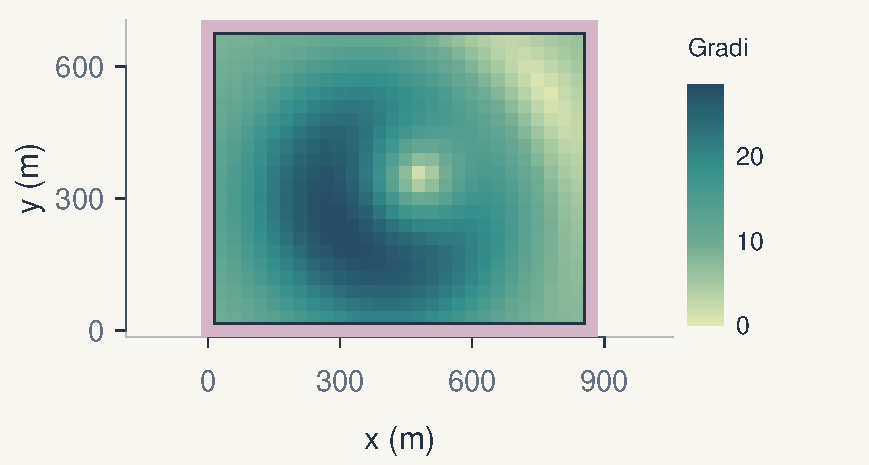
\includegraphics[width=9.85cm,height=5.25cm,keepaspectratio]{Risultati/Figure/41_export_pendenze.pdf}
\vspace{1.5mm}
\PSmall{Griglia completa con 104 celle di bordo NoData. Il riquadro identifica il prodotto interno di 22×28 celle, con passo 30 m.}

\end{minipage}\end{lrbox}
\typeout{FULLBOX:106:PilotLeftBox:\the\ht\PilotLeftBox:\the\dp\PilotLeftBox}

\begin{lrbox}{\PilotRightBox}
\begin{minipage}[t]{7.55cm}\raggedright\color{Ink}\fontsize{11.3}{14.8}\selectfont
\PBody{Il prodotto interno contiene 616 valori. Il prodotto completo conserva invece la griglia 24×30 e 104 celle di bordo NoData.}
\vspace{2.5mm}
\PInfo{La geometria viene costruita dai centri e dai mezzi passi. Esportare la sola matrice senza questi metadati perderebbe la collocazione.}
\PCode{R · ricostruire il raster interno}{106_esempio.R}
\end{minipage}\end{lrbox}
\typeout{FULLBOX:106:PilotRightBox:\the\ht\PilotRightBox:\the\dp\PilotRightBox}

\begin{tikzpicture}[remember picture,overlay]
\PilotChrome{Geometria della pendenza esportata}{IX · CONSEGNA E VERIFICA}{106}{Il raster derivato deve rappresentare gli stessi luoghi ai quali il calcolo si riferisce.}
\node[anchor=north west,inner sep=0] at([xshift=.96cm,yshift=-2.13cm]current page.north west){\usebox{\PilotLeftBox}};
\node[anchor=north west,inner sep=0] at([xshift=11.52cm,yshift=-2.13cm]current page.north west){\usebox{\PilotRightBox}};
\node[anchor=north east,inner sep=0] at([xshift=17.65cm,yshift=-12.06cm]current page.north west){\color{Classical}\fontsize{7.7}{9.2}\selectfont\href{../../03_Notebook_svolti/M12_Tessera/M12_N20.html}{M12\_N20 · notebook svolto}};
\end{tikzpicture}\end{frame}

\begin{frame}[plain]\hypertarget{slide107}{}
\bookmark[level=1,page=107]{Il GeoTIFF conserva geometria e NoData}
\begin{lrbox}{\TitleBox}
\begin{minipage}[t]{17.7cm}\raggedright\color{Ink}\fontsize{11.3}{14.8}\selectfont
\color{Navy}\bfseries\fontsize{20.6}{24.5}\selectfont Il GeoTIFF conserva geometria e NoData
\end{minipage}\end{lrbox}
\typeout{FULLBOX:107:TitleBox:\the\ht\TitleBox:\the\dp\TitleBox}

\begin{lrbox}{\RecallBox}
\begin{minipage}[t]{14.3cm}\raggedright\color{Ink}\fontsize{11.3}{14.8}\selectfont
\fontsize{10.3}{13.8}\selectfont Il file esportato è una parte della consegna: metodo, unità e provenienza devono accompagnarlo.
\end{minipage}\end{lrbox}
\typeout{FULLBOX:107:RecallBox:\the\ht\RecallBox:\the\dp\RecallBox}

\begin{lrbox}{\PilotLeftBox}
\begin{minipage}[t]{10.05cm}\raggedright\color{Ink}\fontsize{11.3}{14.8}\selectfont
{\fontsize{10.2}{13.1}\selectfont\renewcommand{\arraystretch}{1.45}\begin{tabular}{@{}p{3.8cm}p{5.2cm}@{}}\toprule
\textbf{Elemento} & \textbf{Scelta della consegna}\\\midrule
Variabile & Pendenza in gradi\\
Algoritmo & Differenze centrate, quattro vicini\\
Riferimento & EPSG:32632, collocazione fittizia\\
Tipo numerico & FLOAT64 / FLT8S\\
NoData & −9999, distinto dai valori validi\\
Accompagnamento & CSV, metadati e verifiche\\
\bottomrule\end{tabular}}

\end{minipage}\end{lrbox}
\typeout{FULLBOX:107:PilotLeftBox:\the\ht\PilotLeftBox:\the\dp\PilotLeftBox}

\begin{lrbox}{\PilotRightBox}
\begin{minipage}[t]{7.55cm}\raggedright\color{Ink}\fontsize{11.3}{14.8}\selectfont
\PBody{Scriviamo esplicitamente formato numerico e codice mancante. Il GeoTIFF mantiene la geometria, mentre la documentazione conserva il significato scientifico.}
\vspace{2.5mm}
\PSmall{Il percorso mostrato è locale e separato dagli originali.}
\PCode{R · scrittura verificabile}{107_esempio.R}
\end{minipage}\end{lrbox}
\typeout{FULLBOX:107:PilotRightBox:\the\ht\PilotRightBox:\the\dp\PilotRightBox}

\begin{tikzpicture}[remember picture,overlay]
\PilotChrome{Il GeoTIFF conserva geometria e NoData}{IX · CONSEGNA E VERIFICA}{107}{Il file esportato è una parte della consegna: metodo, unità e provenienza devono accompagnarlo.}
\node[anchor=north west,inner sep=0] at([xshift=.96cm,yshift=-2.13cm]current page.north west){\usebox{\PilotLeftBox}};
\node[anchor=north west,inner sep=0] at([xshift=11.52cm,yshift=-2.13cm]current page.north west){\usebox{\PilotRightBox}};
\node[anchor=north east,inner sep=0] at([xshift=17.65cm,yshift=-12.06cm]current page.north west){\color{Classical}\fontsize{7.7}{9.2}\selectfont\href{../../03_Notebook_svolti/M12_Tessera/M12_N20.html}{M12\_N20 · notebook svolto}};
\end{tikzpicture}\end{frame}

\begin{frame}[plain]\hypertarget{slide108}{}
\bookmark[level=1,page=108]{Rileggere verifica ciò che verrà consegnato}
\begin{lrbox}{\TitleBox}
\begin{minipage}[t]{17.7cm}\raggedright\color{Ink}\fontsize{11.3}{14.8}\selectfont
\color{Navy}\bfseries\fontsize{20.6}{24.5}\selectfont Rileggere verifica ciò che verrà consegnato
\end{minipage}\end{lrbox}
\typeout{FULLBOX:108:TitleBox:\the\ht\TitleBox:\the\dp\TitleBox}

\begin{lrbox}{\RecallBox}
\begin{minipage}[t]{14.3cm}\raggedright\color{Ink}\fontsize{11.3}{14.8}\selectfont
\fontsize{10.3}{13.8}\selectfont Il controllo finale deve riguardare il file effettivamente destinato alla consegna.
\end{minipage}\end{lrbox}
\typeout{FULLBOX:108:RecallBox:\the\ht\RecallBox:\the\dp\RecallBox}

\begin{lrbox}{\PilotLeftBox}
\begin{minipage}[t]{10.05cm}\raggedright\color{Ink}\fontsize{11.3}{14.8}\selectfont
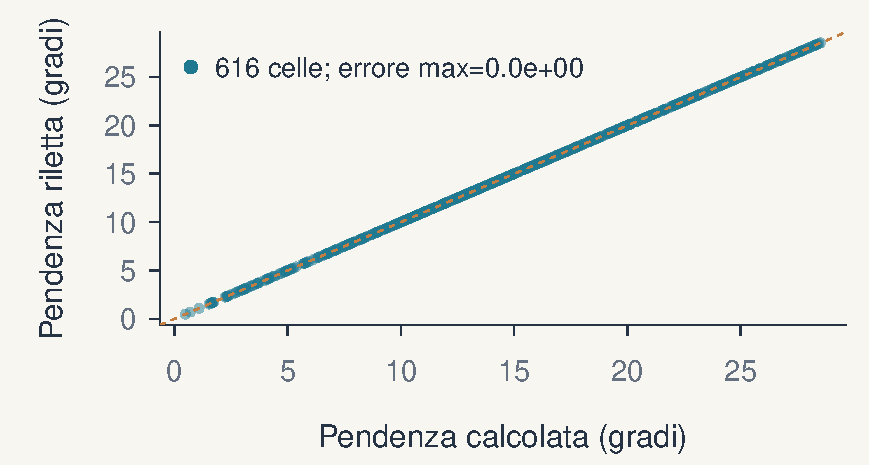
\includegraphics[width=9.85cm,height=5.25cm,keepaspectratio]{Risultati/Figure/42_controllo_roundtrip.pdf}
\vspace{1.5mm}
\PSmall{Confronto fra valori prima della scrittura e dopo la rilettura, insieme ai controlli della geometria e della maschera.}

\end{minipage}\end{lrbox}
\typeout{FULLBOX:108:PilotLeftBox:\the\ht\PilotLeftBox:\the\dp\PilotLeftBox}

\begin{lrbox}{\PilotRightBox}
\begin{minipage}[t]{7.55cm}\raggedright\color{Ink}\fontsize{11.3}{14.8}\selectfont
\PBody{Controlliamo numero di celle, CRS, risoluzione, estensione, NoData e valori. La sola presenza del file non verifica il contenuto.}
\vspace{2.5mm}
\PInfo{Per il prodotto completo verifichiamo anche le 104 celle di bordo mancanti e la corrispondenza delle 616 celle interne.}
\PCode{R · rilettura e confronto}{108_esempio.R}
\end{minipage}\end{lrbox}
\typeout{FULLBOX:108:PilotRightBox:\the\ht\PilotRightBox:\the\dp\PilotRightBox}

\begin{tikzpicture}[remember picture,overlay]
\PilotChrome{Rileggere verifica ciò che verrà consegnato}{IX · CONSEGNA E VERIFICA}{108}{Il controllo finale deve riguardare il file effettivamente destinato alla consegna.}
\node[anchor=north west,inner sep=0] at([xshift=.96cm,yshift=-2.13cm]current page.north west){\usebox{\PilotLeftBox}};
\node[anchor=north west,inner sep=0] at([xshift=11.52cm,yshift=-2.13cm]current page.north west){\usebox{\PilotRightBox}};
\node[anchor=north east,inner sep=0] at([xshift=17.65cm,yshift=-12.06cm]current page.north west){\color{Classical}\fontsize{7.7}{9.2}\selectfont\href{../../03_Notebook_svolti/M12_Tessera/M12_N20.html}{M12\_N20 · notebook svolto}};
\end{tikzpicture}\end{frame}

\begin{frame}[plain]\hypertarget{slide109}{}
\bookmark[level=1,page=109]{I 20 notebook seguono le decisioni della lezione}
\begin{lrbox}{\TitleBox}
\begin{minipage}[t]{17.7cm}\raggedright\color{Ink}\fontsize{11.3}{14.8}\selectfont
\color{Navy}\bfseries\fontsize{20.6}{24.5}\selectfont I 20 notebook seguono le decisioni della lezione
\end{minipage}\end{lrbox}
\typeout{FULLBOX:109:TitleBox:\the\ht\TitleBox:\the\dp\TitleBox}

\begin{lrbox}{\RecallBox}
\begin{minipage}[t]{14.3cm}\raggedright\color{Ink}\fontsize{11.3}{14.8}\selectfont
\fontsize{10.3}{13.8}\selectfont Il codice serve a rendere controllabile l’argomento scientifico, dalla geometria al risultato.
\end{minipage}\end{lrbox}
\typeout{FULLBOX:109:RecallBox:\the\ht\RecallBox:\the\dp\RecallBox}

\begin{lrbox}{\PilotLeftBox}
\begin{minipage}[t]{10.05cm}\raggedright\color{Ink}\fontsize{11.3}{14.8}\selectfont
{\fontsize{10.2}{13.1}\selectfont\renewcommand{\arraystretch}{1.45}\begin{tabular}{@{}p{2.2cm}p{4.9cm}p{1.6cm}@{}}\toprule
\textbf{Notebook} & \textbf{Tema} & \textbf{Slide}\\\midrule
N01–N03 & Griglia, orientamento, GeoTIFF & 5–19\\
N04–N06 & Maschere, dominio e area & 20–32\\
N07–N08, N19 & Aggregazione e allineamento & 33–48\\
N09–N11 & Derivate, pendenza e direzione & 49–66\\
N12 & Illuminazione del rilievo & 67–76\\
N13–N14 & Bande e indice normalizzato & 77–90\\
N15–N17 & Zone, dipendenza e blocchi & 91–102\\
N18, N20 & Finestre ed esportazione & 103–108\\
\bottomrule\end{tabular}}

\end{minipage}\end{lrbox}
\typeout{FULLBOX:109:PilotLeftBox:\the\ht\PilotLeftBox:\the\dp\PilotLeftBox}

\begin{lrbox}{\PilotRightBox}
\begin{minipage}[t]{7.55cm}\raggedright\color{Ink}\fontsize{11.3}{14.8}\selectfont
\PBody{Ogni notebook combina domanda, codice eseguito, risultati e interpretazione. Le risorse necessarie alla lettura sono incorporate negli HTML.}
\vspace{2.5mm}
\PInfo{I collegamenti nei piè di pagina aprono le attività nell’archivio estratto. Il formato R Markdown permette di modificare e rieseguire il lavoro.}
\PBody{Per studiare: dichiarare il risultato atteso, ricostruire il controllo e spiegare quale errore sarebbe in grado di riconoscere.}
\vspace{2.5mm}

\end{minipage}\end{lrbox}
\typeout{FULLBOX:109:PilotRightBox:\the\ht\PilotRightBox:\the\dp\PilotRightBox}

\begin{tikzpicture}[remember picture,overlay]
\PilotChrome{I 20 notebook seguono le decisioni della lezione}{IX · CONSEGNA E VERIFICA}{109}{Il codice serve a rendere controllabile l’argomento scientifico, dalla geometria al risultato.}
\node[anchor=north west,inner sep=0] at([xshift=.96cm,yshift=-2.13cm]current page.north west){\usebox{\PilotLeftBox}};
\node[anchor=north west,inner sep=0] at([xshift=11.52cm,yshift=-2.13cm]current page.north west){\usebox{\PilotRightBox}};
\end{tikzpicture}\end{frame}

\begin{frame}[plain]\hypertarget{slide110}{}
\bookmark[level=1,page=110]{Griglia, metodo e significato restano collegati}
\begin{lrbox}{\TitleBox}
\begin{minipage}[t]{17.7cm}\raggedright\color{Ink}\fontsize{11.3}{14.8}\selectfont
\color{Navy}\bfseries\fontsize{20.6}{24.5}\selectfont Griglia, metodo e significato restano collegati
\end{minipage}\end{lrbox}
\typeout{FULLBOX:110:TitleBox:\the\ht\TitleBox:\the\dp\TitleBox}

\begin{lrbox}{\RecallBox}
\begin{minipage}[t]{14.3cm}\raggedright\color{Ink}\fontsize{11.3}{14.8}\selectfont
\fontsize{10.3}{13.8}\selectfont La geometria della griglia condiziona il significato delle misure che ricaviamo dal territorio.
\end{minipage}\end{lrbox}
\typeout{FULLBOX:110:RecallBox:\the\ht\RecallBox:\the\dp\RecallBox}

\begin{lrbox}{\PilotLeftBox}
\begin{minipage}[t]{10.05cm}\raggedright\color{Ink}\fontsize{11.3}{14.8}\selectfont
\begin{tikzpicture}[x=1cm,y=1cm]
\path[use as bounding box](-.1,-.15) rectangle(9.7,4.8);
\node[pFlow,text width=3.7cm,fill=GeoA!7] (a) at(2.1,3.8){Geometria e supporto};
\node[pFlow,text width=3.7cm,fill=GeoB!7] (b) at(7.3,3.8){Valori e maschere};
\node[pFlow,text width=3.7cm,fill=GeoC!7] (c) at(2.1,1.2){Metodo e scala};
\node[pFlow,text width=3.7cm,fill=GeoA!7] (d) at(7.3,1.2){Risultato e verifica};
\draw[pEdge] (a) -- (b);
\draw[pEdge] (a) -- (c);
\draw[pEdge] (b) -- (d);
\draw[pEdge] (c) -- (d);
\end{tikzpicture}
\PSmall{Riferimenti: documentazione \href{https://rspatial.github.io/terra/}{terra}, \href{https://gdal.org/en/stable/tutorials/geotransforms_tut.html}{GDAL}, \href{https://www.usgs.gov/landsat-missions/landsat-normalized-difference-vegetation-index}{USGS}. Fonti, versioni e verifiche complete accompagnano il pacchetto.}

\end{minipage}\end{lrbox}
\typeout{FULLBOX:110:PilotLeftBox:\the\ht\PilotLeftBox:\the\dp\PilotLeftBox}

\begin{lrbox}{\PilotRightBox}
\begin{minipage}[t]{7.55cm}\raggedright\color{Ink}\fontsize{11.3}{14.8}\selectfont
\PBody{Una buona analisi raster conserva il legame fra la posizione delle celle, il significato dei valori e le trasformazioni applicate.}
\vspace{2.5mm}
\PInfo{Prima di interpretare un risultato, chiedere: cambierebbe con un’altra risoluzione, una maschera diversa o un altro metodo?}
\PBody{La consegna finale rende riconoscibili le scelte e permette di ripetere i controlli sui dati esportati.}
\vspace{2.5mm}

\end{minipage}\end{lrbox}
\typeout{FULLBOX:110:PilotRightBox:\the\ht\PilotRightBox:\the\dp\PilotRightBox}

\begin{tikzpicture}[remember picture,overlay]
\PilotChrome{Griglia, metodo e significato restano collegati}{IX · CONSEGNA E VERIFICA}{110}{La geometria della griglia condiziona il significato delle misure che ricaviamo dal territorio.}
\node[anchor=north west,inner sep=0] at([xshift=.96cm,yshift=-2.13cm]current page.north west){\usebox{\PilotLeftBox}};
\node[anchor=north west,inner sep=0] at([xshift=11.52cm,yshift=-2.13cm]current page.north west){\usebox{\PilotRightBox}};
\end{tikzpicture}\end{frame}

\end{document}
